


%%%%%%%%%%%%%%%%%%%%%%%%%%%%%%%%%%%%%%%%%%%%%%%%%%%%%%%%%%%%%%%%%%%%%%%%%%%%%%%%
% \documentclass[12pt,papel,twoside]{ibtesis}
\documentclass[12pt,screen,twoside]{ibtesis}
% \documentclass[12pt,papel,singlespace,oneside]{ibtesis}
% \documentclass[12pt,papel,preprint,singlespace,oneside]{ibtesis}


%%%%%%%%%%%%%%%%%%%%% Paquetes extra %%%%%%%%%%%%%%%%%%%%%%%%%%%%%%%%%%%%%%%%%%%
% Por conveniencia: aqu\'{\i} puede cargar todos los paquetes y definir los comandos 
% que necesite
%\usepackage{ibextra}

\usepackage[utf8]{inputenc}
\usepackage[T1]{fontenc}             % evita problemas con á/é/ñ en PDF
\usepackage[spanish, english]{babel} % orden = idioma principal primero
\usepackage[dvipsnames]{xcolor} %Si quisieramos poner texto en color
\usepackage{float} %para poner Here en imagen
\usepackage{graphicx} %para insertar imágenes
\usepackage{subfig}
\usepackage{amsfonts}
\usepackage{amsmath}
\usepackage{mathtools}
\usepackage{comment}
\usepackage{xcolor}  
\usepackage{amssymb}
\usepackage{booktabs}
\usepackage{hyperref}
%\usepackage{ibextra}
                % Archivo de bibliografía


%%%%%%%%%%%%%%%%%%%%%%%%%%%%%%%%%%%%%%%%%%%%%%%%%%%%%%%%%%%%%%%%%%%%%%%%%%%%%%%%
%%%%%%%%%%%%%%%%%%%%% Informacion sobre la tesis %%%%%%%%%%%%%%%%%%%%%%%%%%%%%%%
\title{Análisis del Flujo en Convección Mixta en Canales Rectangulares}
\author{Patricio G. Canciani}
\director{Dr. William I. Machaca Abregu}
\codirector{Dr. Federico Teruel}
\carrera{Tesis Carrera de Maestría en Ingeniería}
\grado{Maestrando}
\laboratorio{Departamento de Mecánica Computacional \\ (Centro Atómico Bariloche)}
\jurado{Dr. Christian P. Marcel (Instituto Balseiro -- CNEA)\\ 
Dr. Pablo Garcia Martinez (Instituto Balseiro -- CNEA)\\ 
Dr. César Venier (FCEIA -- SIMEC)\\}

\palabrasclave{Flujo Turbulento,Convección Mixta}
\keywords{Turbulent Flow, Mixed Convection}
% Si queremos poner la fecha manualmente:
% \date{Diciembre de 2099}

%%%%%%%%%%%%%%%%%%%%%%%%%%%%%%%%%%%%%%%%%%%%%%%%%%%%%%%%%%%%%%%%%%%%%%%%%%%%%%%%
%\titlepagefalse % Si no quiere compilar la portada descomente esta linea
%\includeonly{apendices} % Compilar s\'{o}lo estos archivos 
\graphicspath{{figs/}} % Lugar donde encontrar las figuras generales (se puede poner uno en cada cap{\'{\i}}tulo)
%%%%%%%%%%%%%%%%%%%%%%%%%%%%%%%%%%%%%%%%%%%%%%%%%%%%%%%%%%%%%%%%%%%%%%%%%%%%%%%%


\begin{document}

% Dentro del environment 'preliminary' va:
% la dedicatoria, resumen, abstract, indices

\begin{preliminary}

% Escriba su dedicatoria
\dedicatoria{
%A mis padres\\
%A mi hermana\\
%A mis amigos\\
A todos mis seres queridos}

%%% \'{I}ndices %%%%

\begin{abreviaturas}
                                %Abreviaturas
\end{abreviaturas}

\tableofcontents                %\'{I}ndice
\listoffigures                  %Figuras

\listoftables                   %Tablas

\begin{resumen}%

%La convección mixta en canales y conductos verticales se encuentra presente en muchos sistemas de interés, entre ellos los intercambiadores de calor. Este tipo de sistemas pueden presentar cambios de régimen (laminar-turbulento) en su funcionamiento. Desde el punto de vista ingenieril, debido a que parámetros del flujo como el coeficiente de fricción o el número de Nusselt presentan una gran variación. Por ello, en el presente trabajo se estudia la evolución temporal de magnitudes relevantes durante la transición del flujo laminar hacia el turbulento. En particular, se analiza la transición temporal laminar-turbulenta para un canal vertical de placas paralelas sometidos a un flujo de calor constante en las paredes. 
%
%Para estudiar la transición temporal primero resulta necesario conocer el estado inicial laminar
%y el estado final turbulento. En consecuencia, se analizó el flujo turbulento completamente
%desarrollado bajo la influencia de la fuerza boyante. Tanto el estudio del caso completamente desarrollado como la transición temporal se relizó vía simulación numérica directa (DNS) empleando la herramienta numérica Xcompact3D. A partir de estos resultados se estudian magnitudes clave como la energía cinética turbulenta (TKE), la varianza de la temperatura, el número de Nusselt (Nu) y el factor de fricción de Darcy ($f$).  
%
%Para inducir la inestabilidad del flujo laminar hacia uno turbulento se construyen condiciones iniciales empleando análisis de estabilidad lineal. Esto implica resolver un problema de autovalores y autofunciones derivado de las ecuaciones de Orr-Sommerfeld para convección mixta. La resolución de las misma se hace con la herramienta OSCM desarrollada previamente en el grupo (\href{https://github.com/Pato4184/OSMC-Repository}{OSMC-Repository}). Sus soluciones (o combinación de ellas) permiten desencadenar la transición de flujo y comparar la evolución temporal de magnitudes de interés como las mencionada anteriormente. 
%
%En el análisis del régimen turbulento completamente desarrollado, se consideró los número de Reynolds (basado en la velocidad en centro del canal) tales que $ 2100 \leq \text{Re}_o \leq 5000$, los números de Prandtl $\text{Pr}=0\text{.}071,0\text{.}71$ y los números de Richardson tales que $0\text{.}04 \leq \text{Ri}_b \leq 106\text{.}5$. Se emplean aquellos casos con  $\text{Re}_o =5000$, $\text{Pr}=0\text{.}71$ para analizar magnitudes estadísticas de primer orden (perfiles de velocidad y temperatura) y magnitudes de segundo orden (fluctuaciones de velocidad y temperatura, y flujo turbulento de calor). Las estimaciones del número de Nusselt obtenido a partir de nuestras simulaciones concuerdan con correlaciones de la literatura en los rangos de Re, Pr y Ri$_b$ considerados. En particular se encuentró una región ($10^{-6} \lesssim \text{Bo} \lesssim 3 \times 10^{-5}$ siendo Bo el número de boyancia) en la transferencia de calor se reduce respecto al caso puro de convección forzada. Esto último se relaciona a una disminución en la producción de turbulencia cerca las paredes. En el caso del factor de Darcy se propone una correlación propia que muestra buen acuerdo tanto para datos propios como de referencias de otros autores.
%
%Se abordó la transición laminar-turbulenta con $\text{Re}_o=5000$ y $\text{Pr}=0\text{.}71$, considerando dos intensidades de boyancia caracterizadas por $\text{Ri}_b=0\text{.}04$ y $\text{Ri}_b=1\text{.}06$. Se diseñaron condiciones iniciales basadas en el mecanismo de inestabilización propuesto y se identificaron combinaciones de perturbaciones que efectivamente inducen la transición, mostrando que el aumento de la boyancia incrementa la inestabilidad y adelanta la transición para ciertos tipos de perturbaciones. Durante la evolución temporal, los perfiles de velocidad y temperatura presentan pérdidas momentáneas de simetría asociadas a distribuciones no homogéneas de vórtices cerca de las paredes. Las magnitudes TKE, varianza de la temperatura, Nu y $f$ exhiben estados transitorios no monótonos; en el caso con mayor $\text{Ri}_b$ se observa una caída brusca de Nu coincidente con un aumento de TKE y con el aplanamiento del perfil de velocidad producto de la difusión de momento por efecto de la turbulecnia. Aunque la boyancia acelera el desarrollo térmico, en el tiempo simulado Nu no alcanzó el régimen completamente desarrollado en ninguno de los dos casos. Finalmente, la evolución temporal de $\text{Re}_{\tau}$ culmina por encima del valor inicial en el caso de menor $\text{Ri}_b$ y por debajo en el de mayor $\text{Ri}_b$, lo que se explica por cambios del gradiente de velocidad próximo a la pared vinculados al aplanamiento de los perfiles y al incremento súbito de turbulencia.

La convección mixta en canales y conductos verticales está presente en numerosos sistemas de interés, entre ellos los intercambiadores de calor. Estos sistemas pueden presentar cambios de régimen (laminar-turbulento) durante su funcionamiento. Desde el punto de vista ingenieril, esto es relevante porque parámetros del flujo como el coeficiente de fricción o el número de Nusselt pueden experimentar grandes variaciones. Por ello, en el presente trabajo se estudia la evolución temporal de magnitudes relevantes durante la transición del flujo laminar hacia el turbulento. En particular, se analiza la transición temporal laminar-turbulenta para un canal vertical de placas paralelas sometido a un flujo de calor constante en las paredes.

Para estudiar la transición temporal, primero resulta necesario conocer el estado inicial laminar y el estado final turbulento. En consecuencia, se analizó el flujo turbulento completamente desarrollado bajo la influencia de la fuerza boyante. Tanto el estudio del caso completamente desarrollado como la transición temporal se realizó vía simulación numérica directa (DNS) empleando la herramienta numérica Xcompact3D. A partir de estos resultados se estudiaron magnitudes clave como la energía cinética turbulenta (TKE), la varianza de la temperatura, el número de Nusselt (Nu) y el factor de fricción de Darcy ($f$).

Para inducir la inestabilidad del flujo laminar hacia uno turbulento, se construyeron condiciones iniciales empleando análisis de estabilidad lineal. Esto implica resolver un problema de autovalores y autofunciones derivado de las ecuaciones de Orr-Sommerfeld para convección mixta. La resolución de las mismas se realiza con la herramienta OSMC desarrollada previamente en el grupo (\href{[https://github.com/Pato4184/OSMC-Repository}{OSMC-Repository}). Sus soluciones (o combinaciones de ellas) permiten desencadenar la transición del flujo y analizar la evolución temporal de magnitudes de interés como las mencionadas anteriormente.

En el análisis del régimen turbulento completamente desarrollado, se consideraron los números de Reynolds (basados en la velocidad en el centro del canal) tales que $ 2100 \leq \text{Re}_o \leq 5000$, los números de Prandtl $\text{Pr}=0\text{.}071,0\text{.}71$ y los números de \linebreak Richardson tales que $0\text{.}04 \leq \text{Ri}_b \leq 106\text{.}5$. Se emplearon los casos con $\text{Re}_o =5000$, $\text{Pr}=0\text{.}71$ para analizar magnitudes estadísticas de primer orden (perfiles de velocidad y temperatura) y de segundo orden (fluctuaciones de velocidad y temperatura y flujo turbulento de calor). Las estimaciones del número de Nusselt obtenidas a partir de nuestras \linebreak simulaciones concuerdan con correlaciones de la literatura en los rangos de Re, Pr y $\text{Ri}_b$ considerados. En particular, se encontró una región ($10^{-6} \lesssim \text{Bo} \lesssim 3 \times 10^{-5}$, siendo Bo el número de boyancia) en la que la transferencia de calor se reduce respecto del caso puro de convección forzada. Esto último se relaciona con una disminución en la producción de turbulencia cerca de las paredes. Además, se propone una correlación para el factor de Darcy que muestra buen acuerdo tanto con nuestros datos como con referencias de otros autores.

Se abordó la transición laminar-turbulenta con $\text{Re}_o=5000$ y $\text{Pr}=0\text{.}71$, considerando dos intensidades de la fuerza boyante caracterizadas por $\text{Ri}_b=0\text{.}04$ y $\text{Ri}_b=1\text{.}06$. Se diseñaron condiciones iniciales basadas en el mecanismo de inestabilización propuesto y se identificaron combinaciones de perturbaciones que efectivamente inducen la transición, mostrando que el aumento de la flotación incrementa la inestabilidad y adelanta la transición para ciertos tipos de perturbaciones. Durante la evolución temporal, los perfiles de velocidad y temperatura presentan pérdidas momentáneas de simetría asociadas a distribuciones no homogéneas de vórtices cerca de las paredes. Las magnitudes TKE, varianza de la temperatura, Nu y $f$ exhiben estados transitorios no monótonos. En el caso con mayor $\text{Ri}_b$ se observa una caída brusca de Nu, coincidente con un aumento de TKE y con el aplanamiento del perfil de velocidad producto de la difusión de momento por efecto de la turbulencia. Aunque la flotación acelera el desarrollo térmico, en el tiempo simulado Nu no alcanzó el régimen completamente desarrollado en ninguno de los dos casos. Finalmente, la evolución temporal de $\text{Re}_{\tau}$ culmina por encima del valor inicial en el caso de menor $\text{Ri}_b$ y por debajo en el de mayor $\text{Ri}_b$, lo que se explica por cambios del gradiente de velocidad próximo a la pared, vinculados al aplanamiento de los perfiles y al incremento súbito de turbulencia.



\end{resumen}


\begin{abstract}%
\textcolor{red}{NOTA: Hasta que mis directores no le den el okay al resumen en español esta parte no la voy a escribir ...}
\end{abstract}



%%% Local Variables: 
%%% mode: latex
%%% TeX-master: "template"
%%% End: 


\end{preliminary}


% Podemos usar cualquiera de los dos comandos: \input o \include para incluir el texto
\chapter{Introducción}
\label{intro}
%\chapterquote{Hablaban siempre de dinero y planeaban asaltar un banco}{Domingo Cavallo, 2001}

Capitulo introductorio de la tesis


Algunas preguntas clave que deberian responderse en este capitulo:

¿Cuál es el campo general de estudio de tu tesis?

¿Qué fenómeno, problema o sistema estás investigando?

¿Por qué este tema es relevante científica o tecnológicamente?

¿Qué problema específico intenta resolver tu tesis?

¿Cuáles son los objetivos (generales y/o específicos)?

¿Qué enfoque metodológico utilizás? ¿Experimental, teórico, computacional?

¿Cómo está organizada la tesis?

\newpage
\section{Introducción}

\subsection*{Convección Mixta}

Un fluido, en virtud de su masa y velocidad, puede transportar momento. Además, en virtud de su temperatura, puede transportar calor. Estrictamente hablando, la convección es el transporte de energía debido al movimiento global de un medio. Sin embargo, en ingeniería es común utilizar el término convección de forma más amplia para describir la transferencia de calor desde una superficie hacia un fluido en movimiento cuando ambos están a diferentes temperaturas \cite{cengelheat,incropera}. 

La transferencia de calor por convección puede clasificarse según la naturaleza del flujo. Hablamos de convección forzada cuando el flujo es provocado por actores externos como puede ser la acción de bombeo o un gradiente de presión; en cambio, en la convección natural, el flujo es inducido por fuerzas boyantes o de flotación, las cuales se deben a diferencias de densidad producidas por variaciones de temperatura en el propio fluido (Figura \ref{fig:natural_forzada}).

\begin{figure}[H]
 \centering
    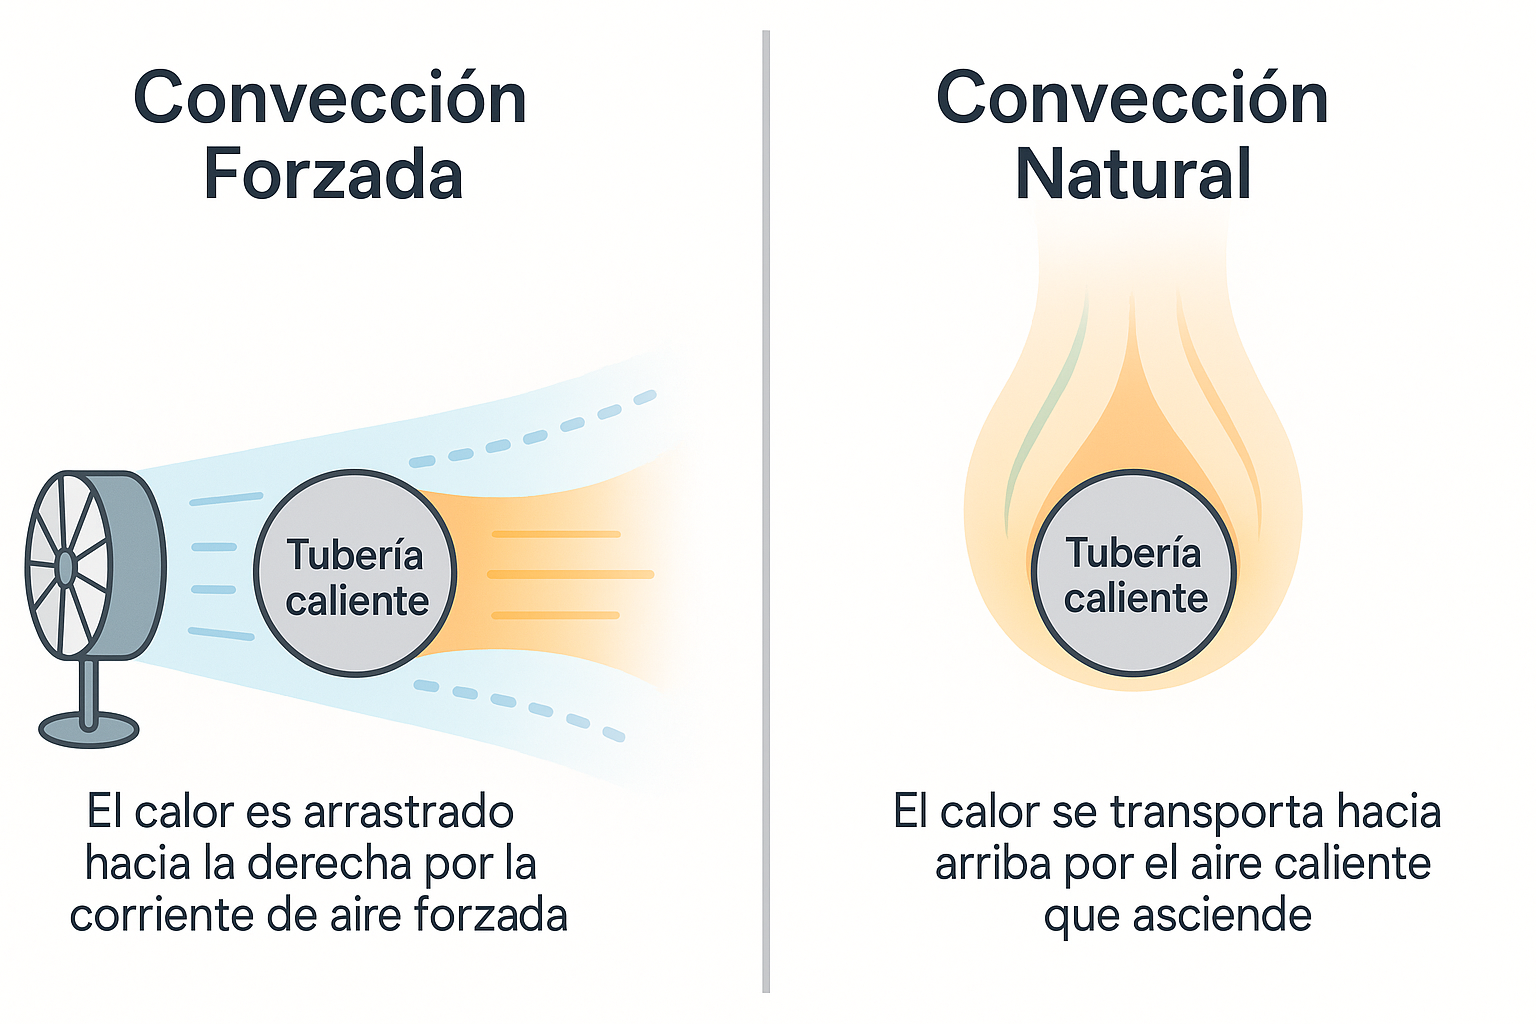
\includegraphics[width=0.6\textwidth]{figures/cap1/natural_forzada.png}
    \label{fig:natural_forzada} 
 \caption{Comparación esquemática de la transferencia de calor alrededor de una tubería caliente: (izquierda) convección forzada; (derecha) convección natural.} 
 \label{fig:natural_forzada}
\end{figure}


Los primeros estudios sobre la transferencia de calor por convección trataron las ramas de la convección forzada y la convección natural de forma separada, sin considerar la posible interacción entre ambas. Por un lado, los experimentos de Henri Bénard (1901) marcaron un hito en la comprensión de la convección natural \cite{benard1901}. Más tarde, Lord Rayleigh (1916) desarrolló la base teórica de la inestabilidad térmica en capas fluidas \cite{rayleigh1916}. En paralelo, en el ámbito de la convección forzada, trabajos como el de Dittus y Boelter (1930) establecieron correlaciones empíricas para la transferencia de calor en tubos \cite{dittus1930}. No fue sino hasta mediados del siglo XX que comenzó a reconocerse que ambos mecanismos pueden coexistir en muchas configuraciones de interés práctico. Así surgió el concepto de convección mixta, donde la convección forzada y la natural actúan simultáneamente como casos extremos de un fenómeno más general \cite{tao1960,metais1964}. 

\subsection*{Régimen de Transición y Transición Laminar-Turbulenta}

Cuando un fluido se desplaza a través de un conducto o sobre una superficie, su movimiento puede clasificarse en dos tipos de régimen: laminar o turbulento. En el régimen laminar, el flujo es ordenado y las partículas del fluido se mueven en capas paralelas sin mezclarse entre sí. En cambio, en el régimen turbulento, el flujo es caótico, con remolinos, tiende a mezclarse, y presenta fluctuaciones en los campos de velocidad y presión. En ese sentido, un flujo que se encuentra en un estado desarrollado\footnote{Esto es, sus magnitudes no varían con el tiempo o con el espacio en un sentido estadístico.} intermedio, de transición , se dice que el flujo está en régimen de transición. Este estado de flujo no debe confundirse con la transición laminar-turbulenta del sistema, donde el flujo evoluciona de un régimen laminar a un régimen turbulento completamente desarrollado. Esta transición puede ocurrir en el tiempo (transición laminar-turbulenta temporal) o en el espacio (transición laminar-turbulenta espacial).

Por otro lado, la transición laminar-turbulenta es un fenómeno de gran importancia para la ingeniería y la física aplicada ya que está presente en diferentes dispositivos termohidráulicos. El cambio de un régimen a otro puede tener un impacto significativo en la transferencia de calor, especialmente en aplicaciones de convección mixta. El coeficiente de fricción (factor de Darcy) o el coeficiente de convección (numéro de Nusselt) se incrementan notablemente cuando se produce la transición \cite{incropera,white}. En ese sentido, este estado no es deseado desde el punto de vista ingenieril ya que es intermitente (es decir, el flujo puede fluctuar entre los regímenes laminar y turbulento), sin embargo, el estudio de la transición es relevante para poder controlar el fenómeno o anticipar, y por tanto aprovechar, su comportamiento. Por ejemplo, un problema importante se da en el diseño de intercambiadores de calor cuando el punto de trabajo del flujo dentro de los tubos o conductos se encuentra en régimen de transición donde las magnitudes relevantes (como coeficientes de fricción y de transferencia de calor) tienen una gran variación \cite{ghajar2019heat}.

La evolución de un flujo, tanto en el tiempo como en el espacio, depende de las perturbaciones externas que reciba (por ejemplo, cambios de presión o de temperatura), de las condiciones de borde a las que esté sometido (como puede ser la rugosidad, flujo de calor en las paredes o gradientes de presión, entre otros) y de la respuesta del propio sistema, determinada por sus propiedades físicas y el régimen de flujo. Para modelar matemáticamente las condiciones que pueden modificar ese régimen —es decir, los estados iniciales capaces de desencadenar una transición— y analizar cómo dicha transición impacta en la transferencia de calor, se recurre a la teoría de estabilidad hidrodinámica. Esta teoría ofrece un marco para predecir cuándo un flujo laminar se volverá inestable mediante el estudio de la evolución de pequeñas perturbaciones: si estas crecen en el espacio o en el tiempo, el flujo pierde su estabilidad y eventualmente transiciona hacia un régimen turbulento.

La investigación teórica sobre la transición ha tenido un desarrollo histórico notable que se remonta al siglo XIX, con el célebre experimento de Osborne Reynolds \cite{reynolds1883}, que marcó el inicio del estudio sistemático del fenómeno. A comienzos del siglo XX, Orr \cite{orr1907} y Sommerfeld \cite{sommerfeld1908} formalizaron las bases de la estabilidad hidrodinámica al desarrollar las ecuaciones linealizadas que llevan sus nombres, conocidas como ecuaciones de Orr-Sommerfeld. Estas describen la evolución de perturbaciones en un flujo y son fundamentales para comprender los mecanismos de transición. Un avance crucial se produjo con los trabajos de Tollmien \cite{tollmien1930} y Schlichting \cite{schlichting1933}, quienes describieron de forma teórica el estado lineal de la transición; esta teoría fue confirmada experimentalmente en el estudio de la capa límite sobre una placa plana realizado por Schubauer y Skramstad \cite{schubauer1947laminar}. Finalmente, la incorporación de la teoría de inestabilidad secundaria por Herbert \cite{herbert1983secondary} permitió extender el análisis al caso tridimensional, ofreciendo así una comprensión más completa del fenómeno.


\section{Motivación}

En la actualidad, muchos problemas de ingeniería presentan flujos en régimen de transición. La mayoría de los flujos en estás condiciones son no isotérmicos \cite{chen2003direct}. El estudio de la transferencia de calor en la transición laminar-turbulenta es importante en diversas aplicaciones ingenieriles, como en los elementos combustibles de reactores nucleares, en intercambiadores de calor, en los álabes de una turbina, equipos electrónicos, entre otros.

Por otro lado, el fenómeno de convección mixta puede manifestarse conjuntamente en flujos atmosféricos \cite{pirozzoli2017mixed} como también en aplicaciones de ingeniería presentes en el proceso de fabricación de silicio, la refrigeración de equipos electrónicos, paneles solares térmicos, álabes de turbinas, intercambiadores de calor de diverso tipo, reactores nucleares, entre otros \cite{kasagi1997direct}. 

Entre las aplicaciones técnicas de mayor relevancia de la convección mixta se destaca el transporte de energía térmica. En las últimas décadas se han realizado muchos esfuerzos para desarrollar técnicas tendientes a mejorar la transferencia de calor y el desempeño global de los intercambiadores de calor. El interés en estas técnicas radica en el ahorro de la energía. En este sentido, las necesidades energéticas actuales propician el diseño y la mejora constante de los reactores nucleares utilizados para la provisión de energía eléctrica. Dentro de la nueva generación de reactores nucleares GEN-IV\footnote{\url{https://www.gen-4.org/}}, de los seis conceptos especificados, uno corresponde a reactores tipo GFR (\textit{Gas-cooled Fast Reactor}) que utiliza como refrigerante gas helio cuyo número de Prandtl es Pr$\simeq0.7$ similar al aire.


\section{Objetivos}

El objetivo del presente trabajo es el estudio de la transferencia de calor en régimen de transición laminar-turbulenta en convección mixta. Para ello se emplea la herramienta numérica Incompact3D. Se obtienen resultados numéricos para números de Reynolds entre $2000$ y $5000$, números de Prandt igual a $0.071$ y $0.71$ y numéros de Richardson entre $0.04$ y $106$.

Parte de las tareas secundarias para la realización de trabajo incluyeron:

\begin{itemize}

	\item Entrenamiento y manejo en el uso de la herramienta numérica Incompact3D.
	
	\item Validación de la herramienta numérica y simulación de flujos turbulentos.

	\item Validación de l de métodos para inestabilizar soluciones laminares en la herramienta
numérica.

\end{itemize}

\textcolor{red}{No se como escribir esta parte. Como escribir el uso y validación de la herramienta de Szuban y todo lo demas que queda referido a los objetivos.}





\section{Organización del trabajo}
\chapter{Modelo Matemático} \label{cap:modelo}

En este capítulo se presenta el marco teórico que sustenta este trabajo. Se introduce brevemente el concepto de turbulencia y de simulaciones DNS. Luego, se describen las ecuaciones, junto con las condiciones de borde, empleadas para modelar el sistema físico bajo análisis: un canal de placas paralelas sometido a un flujo de calor constante en las paredes. Asimismo, se definen las magnitudes estadísticas necesarias para el tratamiento de los datos obtenidos mediante simulaciones.

Por otra parte, se incluye un breve resumen del análisis de estabilidad lineal que constituye la base teórica para el cálculo numérico de los autovalores y autofunciones empleados en la construcción de las perturbaciones utilizadas para inestabilizar flujos con convección mixta. Estas perturbaciones se aplican en el Capítulo \ref{cap:transicion}, donde se analiza la transición temporal laminar–turbulenta.

\section{El concepto de turbulencia. Simulaciones Numéricas Directas (DNS)}

Los flujos se clasifican, de manera general, en laminares, de transición y turbulentos. La mayoría de los flujos presentes en la naturaleza y en aplicaciones industriales son turbulentos, por lo que su estudio tiene un gran interés tanto en el ámbito científico como en el tecnológico. Algunos ejemplos de flujo turbulento se encuentran presentes en el movimiento de las nubes en el cielo, las corrientes oceánicas, el flujo sobre el ala de un avión o el flujo sobre el álabe de una turbina, entre muchos otros.

Todos estos flujos presentan un comportamiento aparentemente aleatorio y caótico, lo cual se refleja en las variaciones espaciales y temporales de las variables del flujo, tales como la velocidad, la temperatura o la densidad. Las complejidades inherentes a la turbulencia dificultan su definición de forma concisa; por ello, en general, no es común dar una definición de turbulencia sino más bien presentar ciertos atributos canónicos \cite{smits2009lectures}:

\begin{itemize}
	
	\item \textbf{Tridimensionalidad.} La turbulencia es un fenómeno inherentemente tridimensional. 
	
	\item \textbf{Naturaleza no estacionaria.} Los flujos turbulentos evolucionan en el tiempo y se caracterizan por variaciones inestables en magnitudes asociadas (velocidad, presión, temperatura, etc).
	
	\item \textbf{Carácter multiescala.} La turbulencia involucra una amplia gama de escalas en el espacio y en el tiempo. 
	
	\item \textbf{Difusividad.} Se tiene una mezcla eficaz\footnote{El término ``mezcla eficaz'' se refiere a la capacidad de un flujo turbulento para mezclar y dispersar las diferentes propiedades del fluido de manera rápida y homogénea.} de todas las propiedades del fluido (masa, velocidad, temperatura, concentración, etc.).

\end{itemize}

Por su relevancia práctica y su naturaleza aleatoria y compleja, este fenómeno ha sido objeto de un gran número de investigaciones teóricas y experimentales a lo largo de los últimos dos siglos. Incluso en la actualidad, se sigue estudiando con el objetivo de entender mejor su complejidad. En este contexto, el uso de la computación para resolver las ecuaciones que gobiernan la dinámica de fluidos ha adquirido un papel preponderante y se ha consolidado como una de las herramientas más utilizadas para el análisis de flujos turbulentos.

El rápido progreso de las computadoras de alto rendimiento, permite que la simulación numérica directa (\textit{Direct Numerical Simulation}, DNS) sea una herramienta fundamental para la investigación de la turbulencia \cite{moin1998direct}. Esta permite calcular la solución tridimensional y no estacionaria de las ecuaciones de conservación involucradas. Al resolverse sin recurrir a modelos de turbulencia, estas simulaciones requieren una precisión elevada para capturar todas las escalas del flujo \cite{pope2001turbulent}.

\section{Descripción del sistema bajo estudio. Ecuaciones de Gobierno}

Se considera el sistema representado en la Figura \ref{fig:sistem_domain} donde la dinámica de un fluido viscoso e incompresible sucede entre dos paredes paralelas e infinitas ubicadas en $y=\pm d$. Esto constituye un canal vertical de placas paralelas donde ambas paredes están sometidas a un flujo de calor constante $q''_w$.

\begin{figure}[H]
 \centering
  \subfloat[]{
    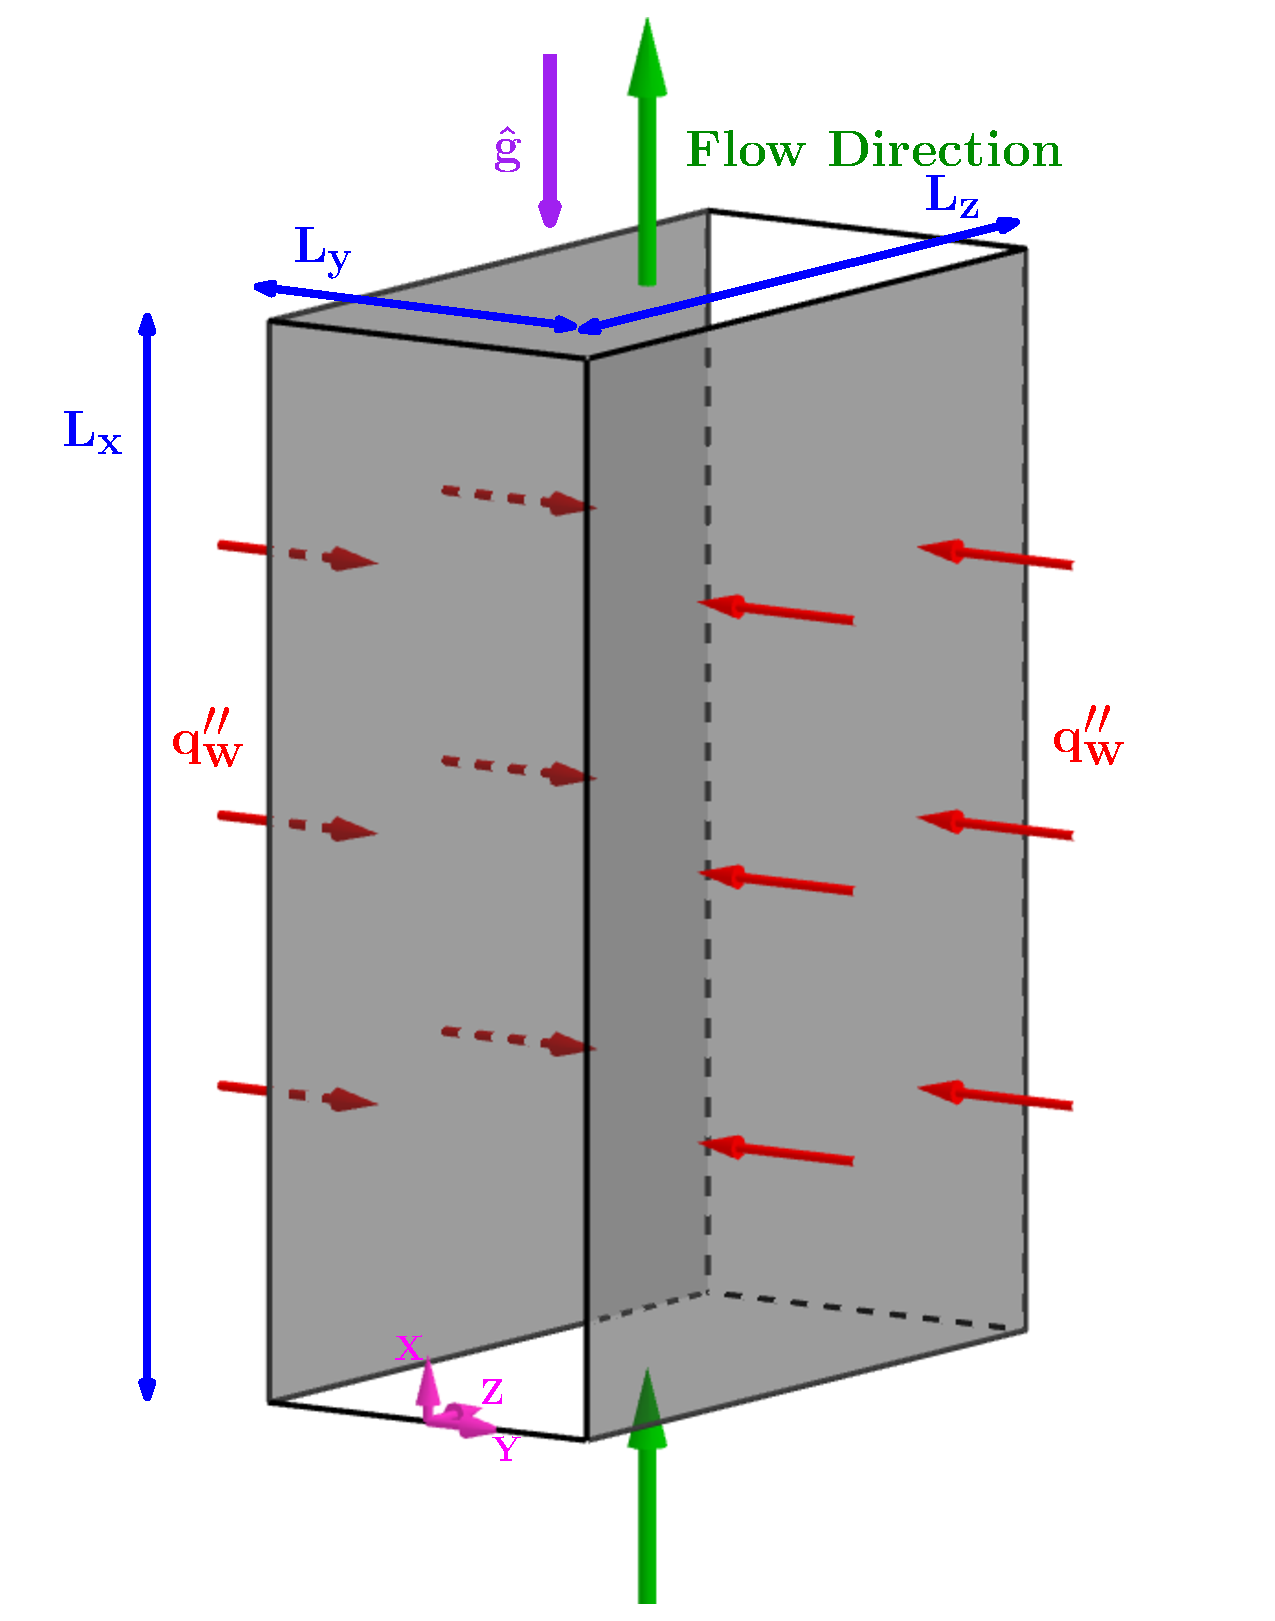
\includegraphics[width=0.49\textwidth]{figures/cap2/domain3d.eps}
    \label{fig:dom3d}}  
    \subfloat[]{
    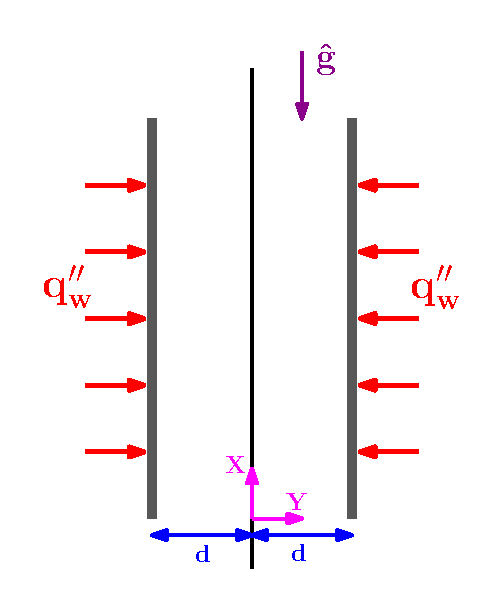
\includegraphics[width=0.49\textwidth]{figures/cap2/domain2d.eps}
    \label{fig:dom2d}}  
 \caption{Esquema del sistema físico bajo análisis.} 
 \label{fig:sistem_domain}
\end{figure}

El flujo ocurre en la dirección de la corriente (\textit{streamwise}) paralelo al eje X y su sentido es opuesto a la aceleración de la gravedad. Esta configuración se conoce como flujo ascendente o \textit{aiding flow}. Las ecuaciones de gobierno corresponden a los principios de conservación de masa, momento y energía que se expresan en el cuadro \ref{eq:gob_system}.

\begin{equation}
        \boxed{ \begin{array}{lcc}
			  %\\
              &  \nabla \cdot \left( \rho_o \mathbf{u} \right) = 0 \\
              \vspace*{2mm}
              &  \frac{\partial \left( \rho_o \mathbf{u} \right)}{\partial t} + \mathbf{u} \cdot \nabla  \left( \rho_o \mathbf{u} \right) = -\nabla \text{p} + \mu_o \hspace{1mm} {\nabla}^2 \mathbf{u}  + \rho(T) \hspace{1mm} \mathbf{g} \\
              \vspace*{2mm}
              &  \frac{\partial T}{\partial t} + \mathbf{u} \cdot \nabla T =  \alpha \hspace{1mm} \nabla^2 T  \\
              % \\
             \end{array}
               }
             \label{eq:gob_system}
\end{equation}

Un sistema físico cuyas dimensiones ``son muy grandes'' (o infinitas) constituye un sistema ideal. En él, es posible ubicar el origen de nuestro sistema de referencia lejos de los extremos a fin de evitar efectos de bordes. Allí, el flujo se encuentra completamente desarrollado y ha alcanzado un estado estadísticamente estacionario, es decir, sus valores estadísticos, como el promedio o la varianza, no varían en el tiempo. En este contexto, la condición de flujo de calor constante en las paredes se imponen como condiciones de Neumann:

\begin{equation}
\kappa \hspace{0.5mm} \left. \frac{\partial T}{\partial y} \right\vert_{y=\mp d} = \pm q''_w \text{.}
\label{eq:neumann}
\end{equation}

Debido a una limitación computacional evidente, nuestro modelo no puede abarcar dicha extensión. En ese sentido, el ``dominio infinito'' se reemplaza con un dominio acotado de dimensiones $L_x \times L_y \times L_z$ (Figura \ref{fig:dom3d}) adoptando condiciones de borde periódicas (PBC) en la direcciones $X$ y $Z$:
\begin{align}
\xi(x=0,y,z,t) &= \xi(x=L_x,y,z,t)
\label{eq:pbc1} \\
\xi(x,y,z=0,t) &= \xi(x,y,z=L_z,t)
\label{eq:pbc2}
\end{align}
siendo $\xi$ un campo escalar arbitrario. Esto se puede interpretar como si las PBC crearan ``la ilusión'' de un dominio infinito, mediante la repetición de este dominio finito en el espacio.

Por otra parte, como se ha mencionado, dado que un flujo turbulento no es estacionario, aparecen fluctuaciones del flujo de calor y de la temperatura sobre la superficie de la pared. En este contexto, algunos autores \cite{kasagi1992direct,tao1960} asumen que dichas fluctuaciones son pequeñas a fin de considerar que la temperatura en la pared es localmente isotérmica y que además, el flujo de calor no varía en la dirección de la corriente. Eso equivale a suponer que la temperatura en la pared, promediada en el tiempo y en la dirección $Z$, crece linealmente con la coordenada $x$, y por lo tanto: 

$$
\langle T_w \rangle = \mathcal{A} \hspace{0.5mm} x.
$$

Debido al crecimiento lineal de $\langle T_w \rangle$, es requerido realizar el cambio de variable $T(x,y,z,t) = \langle T_w \rangle - \theta(x,y,z,t)$ para que sigan siendo válidas las condiciones de borde periódicas (ecuaciones \ref{eq:pbc1} y \ref{eq:pbc1}). Dicha modificación introduce un término fuente en la ecuación de conservación de energía:

\begin{equation}
\frac{ \partial \theta }{ \partial t } + \mathbf{u} \cdot \nabla \theta = \alpha \nabla^2 \theta + \mathcal{A} \hspace{0.5mm} u_x 
\label{eq:energy_pcb_source}
\end{equation}

Asimismo, se emplea la aproximación de Bousinessq que supone que los cambios de densidad en el fluido pueden despreciarse, excepto donde la densidad está multiplicada por $\mathbf{g}$ \cite{kundu}. El término $\rho(T) \mathbf{g}$ de la ecuación de momento se reescribe según la expresión \ref{eq:bussinesq}, donde $\rho_o \equiv \rho(T_R)$ y $\rho_w \equiv \rho(T=\langle T_w \rangle)$ \cite{incropera}. Luego, la ecuación de momento queda reescrita como se expresa en la ecuación \ref{eq:mom_rewrite} siendo $\mathbf{\hat{e_g}}=(-1,0,0)$, $\rho_{w/2} \equiv \rho(T=\langle T_w \rangle / 2)$ y $C$ es una constante que no depende de $x$.

\begin{equation}
\begin{aligned}
\rho(T) \mathbf{g} &= \rho_o \left[ 1 - \beta (T - T_R) \right] \mathbf{g} \\
				   &= \rho_o \left[ 1 - \beta ( \hspace{0.5mm} (\langle T_w \rangle - \theta) - T_R) \right] \mathbf{g} \\
 		           &= \rho_o \beta \theta \mathbf{g} + \rho_w \mathbf{g}
\end{aligned}
\label{eq:bussinesq}
\end{equation}

\begin{equation}
\frac{ \rho_o \hspace{0.5mm} \partial \mathbf{u}}{\partial t} + \mathbf{u} \cdot \nabla  \left( \rho_o \mathbf{u} \right) = -\nabla \left[ \text{p} + \rho_{w/2} \hspace{0.5mm} g \hspace{0.5mm} x + C \right] + \mu_o \hspace{1mm} {\nabla}^2 \mathbf{u}  + g \hspace{0.5mm} \rho_o \hspace{0.5mm} \beta \hspace{0.5mm} \theta \hspace{0.5mm} \mathbf{\widehat{e_g}},
\label{eq:mom_rewrite}  
\end{equation}
%\rho_w \hspace{0.5mm} g \hspace{0.5mm} \mathbf{\widehat{e_g}}
 

Mediante el balance de energía en el volumen de control $L_x \times L_y \times L_z$, es posible demostrar que $\mathcal{A} = \frac{q''_w}{\rho_o  c_p U_b d}$ siendo $d$ el semiancho del canal y $U_b$ la velocidad \textit{bulk} \cite{pope2001turbulent}. Luego, empleando la velocidad en el centro del canal $U_o$, el semiancho $d$, la temperatura $T_o = \mathcal{A} \hspace{0.3mm} d $ y tomado $\text{p}^* = \left[ \text{p} + \rho_{w/2} \hspace{0.5mm} g \hspace{0.5mm} x + C \right] / \rho_o (U_o)^2$, el sistema de ecuaciones dimensional \ref{eq:gob_system} queda escrito en su forma adimensional como se muestra en el cuadro \ref{eq:gob_system_adim}. Los números adimensionales asociados a estas ecuaciones, se expresan en las relaciones \ref{eq:num_adim}, de izquierda a derecha, se tiene: el número de Reynolds, el número de Prandtl, el parámetro que acompaña al término boyante y al número de Richardson basado en el flujo de calor. 

Otro detalle importante es el hecho de que el fluido de trabajo es impulsado por un caudal másico constante. Esta cuestión se encuentra representada por el término fuente $f \hspace{0.3mm} \mathbf{\widehat{e_x}}$, en la ecuación de momento, donde $f$ es una constante en el espacio y varía con el tiempo de manera que mantiene constante el caudal total. 

\begin{equation}
\boxed{
\begin{array}{l}
    \nabla^* \cdot \mathbf{u^*} = 0 \\
    \frac{\partial \mathbf{u^*}}{\partial t^*} + \mathbf{u^*} \cdot \nabla^* \mathbf{u^*} = 
    -\nabla \text{p}^* + \frac{1}{\text{Re}_o} \hspace{0.5mm} \nabla^{*2} \mathbf{u^*} + \Pi \hspace{0.5mm} \theta^* \hspace{0.5mm} \mathbf{\widehat{e_g}} + f \mathbf{\widehat{e_x}}  \\
    \frac{\partial \theta^*}{\partial t^*} + \mathbf{u^*} \cdot \nabla^* \theta^* = 
    \frac{1}{\text{Re}_o \hspace{0.5mm} \text{Pr}} \hspace{0.5mm} \nabla^{*2} \theta^* + u_x^* 
\end{array}
}
\label{eq:gob_system_adim}
\end{equation}

\begin{equation}
\text{Re}_o = \frac{\mu_o}{\rho_o \hspace{0.5mm} U_o \hspace{0.5mm} d } \quad ; \quad \text{Pr}= \frac{\mu_o}{\rho_o \hspace{0.5mm} \alpha} \quad ; \quad \Pi = \frac{\text{Ri}_o}{\text{Re}_o \hspace{0.5mm} \text{Pr}} \quad ; \quad \text{Ri}_o = \frac{g \hspace{0.5mm} \beta \hspace{0.5mm} q''_w \hspace{0.5mm} d^2}{k \hspace{0.5mm} U_o^2}
\label{eq:num_adim}
\end{equation}
%siendo Ra, el número de Rayleigh.

Las condiciones de flujo de calor constante en las paredes se expresean, en su forma adimensional, en la ecuación \ref{eq:neumann_adim}. Sin embargo, estas condiciones pueden ser aproximadas como condiciones de Dirichlet ya que al suponer que la temperatura de las paredes es constante (fluctuaciones de temperatura despreciables) se obtiene: 
$$T(x,y=-d,z,t) = T(x,y=+d,z,t) = \langle T_w \rangle$$ 
Éste tipo de aproximación se conoce en la literatura como \textit{Mixed Boundary Condition} \cite{straub2019influence} y su forma adimensional se expresa en la ecuación \ref{eq:dirichlet_adim_theta}. Por último, para las componentes de la velocidad y del campo de presión, se adoptan condiciones de no deslizamiento y condiciones de Neumann homogéneas, respectivamente, en las paredes. 

\begin{align}
\begin{array}{l}
    \left. \frac{\partial \theta^*}{\partial y^*} \right\vert_{y^*=-1} = + \frac{2}{3} \text{Re}_o \hspace{0.5mm} \text{Pr} \\
    \left. \frac{\partial \theta^*}{\partial y^*} \right\vert_{y^*=+1} = - \frac{2}{3} \text{Re}_o \hspace{0.5mm} \text{Pr} 
\end{array}
\label{eq:neumann_adim}
\end{align}

\begin{equation}
\theta^*(x^*,y^*=0,z^*,t^*) = \theta^*(x^*,y^*=2,z^*,t^*) = 0
\label{eq:dirichlet_adim_theta}
\end{equation}



\subsection{Sumario de Ecuaciones}

\textbf{Ecuaciones de Gobierno:}
\begin{equation}
\begin{array}{l}
    \nabla^* \cdot \mathbf{u^*} = 0 \\
    \frac{\partial \mathbf{u^*}}{\partial t^*} + \mathbf{u^*} \cdot \nabla^* \mathbf{u^*} = 
    -\nabla \text{p}^* + \frac{1}{\text{Re}_o} \hspace{0.5mm} \nabla^{*2} \mathbf{u^*} + \frac{\text{Ri}_o}{\text{Re}_o \hspace{0.5mm} \text{Pr}} \hspace{0.5mm} \theta^* \hspace{0.5mm} \mathbf{\hat{g}} + f \mathbf{\widehat{e_x}}  \\
    \frac{\partial \theta^*}{\partial t^*} + \mathbf{u^*} \cdot \nabla^* \theta^* = 
    \frac{1}{\text{Pr}}\hspace{0.5mm}  \frac{1}{\text{Re}_o} \hspace{0.5mm} \nabla^{*2} \theta^* + u_x^* 
\end{array}
\label{eq:gob_system_res1}
\end{equation}

\textbf{Condiciones de borde:} considerando $\xi= u^*_x, u^*_y, u^*_z, \text{p}^*, \theta^*$, entonces
\begin{align}
&\xi(x^*=0,y^*,z^*,t^*) = \xi(x^*=L_x/d,y^*,z^*,t^*) 
	\label{eq:bc_1} \\
&\xi(x^*,y^*,z^*=0,t^*) = \xi(x^*,y^*,z^*=L_z/d,t^*) 
	\label{eq:bc_2} \\
&\theta^*(x^*,y^*=-1,z^*,t^*)       = \theta^*(x^*,y^*=+1,z^*,t^*) = 0
	\label{eq:bc_3} \\
&\mathbf{u^*}(x^*,y^*=-1,z^*,t^*)   = \mathbf{u^*}(x^*,y^*=+1,z^*,t^*) = 0
	\label{eq:bc_4} \\
&\partial_y \text{p}^*(x^*,y^*=-1,z^*,t^*) = \partial_y \text{p}^*(x^*,y^*=+1,z^*,t^*) = 0
	\label{eq:bc_5}
\end{align}

A lo largo de este trabajo, particularmente para el análisis de estabilidad lineal, se utiliza también la forma adimensional de las ecuaciones del trabajo de Chen \cite{chen1996linear} que se obtienen empleando el  semiancho del canal $d$, la velocidad \textit{bulk} $U_b$ y la temperatura $T_c = \text{Re} \hspace{0.5mm} \text{Pr} \hspace{0.5mm} \mathcal{A} \hspace{0.5mm} d$. Dichas ecuaciones se expresan en \ref{eq:gob_system_res2}. Las condiciones de borde son exactamente análogas a su forma adimensional de más arriba. Adicionalmente, aparece otro número adimensional conocido: el número de Rayleigh (Ra) basado en el flujo de calor y definido en la ecuación \ref{eq:Rayleigh}.

\begin{equation}
\begin{array}{l}
    \nabla^* \cdot \mathbf{v^*} = 0 \\
    \frac{\partial \mathbf{v^*}}{\partial t^*} + \mathbf{v^*} \cdot \nabla^* \mathbf{v^*} = 
    -\nabla \text{p}^* + \frac{1}{\text{Re}_b} \hspace{0.5mm} \nabla^{*2} \mathbf{u^*} + \frac{\text{Ra}}{\text{Re}_b} \hspace{0.5mm} \varphi^* \hspace{0.5mm} \mathbf{\hat{g}} + f \mathbf{\hat{x}} \\
    \frac{\partial \varphi^*}{\partial t^*} + \mathbf{v^*} \cdot \nabla^* \varphi^* = 
    \frac{1}{\text{Pr}}\hspace{0.5mm}  \frac{1}{\text{Re}_b} \hspace{0.5mm} \left[ \nabla^{*2} \varphi^* - v_x^* \right]  
\end{array}
\label{eq:gob_system_res2}
\end{equation}

\begin{equation*}
\varphi^* = -  \frac{\theta^*}{\text{Re}_o \hspace{0.5mm} \text{Pr}}  \quad ; \quad \mathbf{v^*} = \frac{2}{3} \mathbf{u^*} \quad ; \quad \text{Re}_b = \frac{2}{3} \text{Re}_o
\end{equation*}  

\begin{equation}
\text{Ra} = \frac{g \hspace{0.5mm} \beta \hspace{0.5mm} q''_w \hspace{0.5mm} d^3}{c_p \hspace{0.5mm} \alpha \hspace{0.5mm} \mu_o \hspace{0.5mm} U_b}
\label{eq:Rayleigh}
\end{equation} 


\section{Magnitudes estadísticas de flujos turbulentos} \label{sec:mag-stat}

En flujos turbulentos, los campos como la velocidad son variables aleatorias \\ \cite{pope2001turbulent}. Supóngase que $\xi$ es un campo arbitrario asociado al sistema. Para una posición e instante determinados en un experimento (o simulación) repetible bajo las mismas condiciones, y sin dependencia entre repeticiones, el conjunto $\lbrace \xi^{(1)}, \xi^{(2)}, \cdots \rbrace$ puede considerarse de variables i.i.d. (independientes e idénticamente distribuidas). Entonces, el promedio en ensemble sobre $N$ repeticiones se define como 

\begin{equation*}
\langle \xi \rangle_N = \frac{1}{N} \sum^N_{n=1} \xi^{(n)} 
\end{equation*}
siendo $N$ muy grande. Si el sistema es estadísticamente estacionario, sus propiedades estadísticas no cambian con el tiempo; si es estadísticamente homogéneo, no varían con la posición; y si es ergódico \cite{moser2003}, el promedio en ensemble puede reemplazarse por el promedio en el tiempo y/o en el espacio (direcciones homogéneas). 

En problemas de turbulencia, los promedios y las fluctuaciones de las variables de interés son importantes, por lo que la descomposición de Reynolds \cite{pope2001turbulent, kundu} de la variable instantánea arbitraria $\xi$ puede representarse como un valor promedio $\langle \xi \rangle$ y una fluctuación $\xi^{\prime}$:

$$\xi = \langle \xi \rangle + \xi^{\prime}$$
donde $\langle (\text{.}) \rangle$ denota el promedio estadístico y $(\text{.})^{\prime}$ denota la parte fluctuante. 

Supongase entonces, que $\eta$ es otra magnitud instantánea del flujo. El promedio de la multiplicación  de las fluctuaciones de $\xi$ y $\eta$ son cantidades de interés para la construcción de modelos de turbulencia \cite{pope2001turbulent}. Dichas cantidades nos indican que tan correlacionadas están $\xi$ y $\eta$ entre sí. Estas se obtienen a partir del promedio de las magnitudes totales, ecuación \ref{eq:mag-cov}, donde se usa el hecho de que el promedio de una fluctuación es nulo y el promedio de otro promedio sigue siendo él mismo \cite{pope2001turbulent}. De esta manera, el promedio del producto de fluctuaciones $\langle \xi^{\prime} \eta^{\prime} \rangle$ queda expresado en la ecuación \ref{eq:fluct-corr}.

\begin{equation}
\begin{aligned}
\langle \xi \eta \rangle &= \langle (\langle \xi \rangle + \xi^{\prime}) (\langle \eta \rangle + \eta^{\prime}) \rangle \\
                         &= \langle \xi \rangle \langle \eta \rangle + \langle \xi^{\prime} \eta^{\prime} \rangle
\end{aligned}
\label{eq:mag-cov}
\end{equation}

\begin{equation}
\langle \xi^{\prime} \eta^{\prime} \rangle = \langle \xi \eta \rangle - \langle \xi \rangle \langle \eta \rangle
\label{eq:fluct-corr}
\end{equation}

Algunas cantidades importante que aparecen en las ecuaciones promediadas de conservación (ecuaciones RANS \cite{kundu}) son:

\begin{itemize}
	\item $\langle u^{\prime}_i u^{\prime}_j \rangle$: componentes del tensor de Reynolds con $i,j=x,y,z$;
	\item $\langle \theta^{\prime} u^{\prime}_i \rangle$: flujos turbulentos de calor en la dirección $i$, con $i=x,y,z$;
	\item $\langle \theta^{\prime} \theta^{\prime} \rangle$: varianza de la temperatura;

	\item otra magnitud utilizada ampliamente a lo largo de este trabajo es la energía cinética turbulenta $k$ (o TKE) definida como proporcional a la traza del tensor de Reynolds, esto es, 

\begin{equation}
k = \frac{1}{2} \left[ \langle u^{\prime}_x u^{\prime}_x \rangle + \langle u^{\prime}_y u^{\prime}_y \rangle + \langle u^{\prime}_z u^{\prime}_z \rangle \right] \text{.}
\label{eq:tke}
\end{equation}

\end{itemize}


\section{Teoría de Estabilidad Lineal. Perturbaciones} \label{line_an}

La evolución de un flujo laminar a uno turbulento (transición laminar-turbulenta) es crucial en ingeniería ya que las características del mismo varían notablemente entre estos regímenes. Por ejemplo, los coeficientes de fricción y de convección aumentan considerablemente al pasar de un régimen laminar a uno turbulento \cite{machaca2024}. Las ecuaciones de Navier–Stokes admiten ambas soluciones bajo ciertos requisitos, lo que implica que el tipo de flujo y su evolución dependen de las perturbaciones y las condiciones impuestas sobre el sistema. 

Para analizar la estabilidad lineal y prever de forma matemática cómo cambiará el flujo una vez perturbado, resulta indispensable conocer el flujo base sobre el que se añaden las perturbaciones para desencadenar las inestabilidades que dan paso a la transición. En este trabajo se adopta como flujo base al flujo laminar completamente desarrollado. %En consecuencia, la evolución de las perturbaciones también queda condicionada por dicho estado inicial. 



\subsection{Flujo Base}

Si el flujo está completamente desarrollado, tanto térmica como hidrodinámicamente, entonces el mismo sólo dependerá de la variable $y^*$. El sistema de ecuaciones \ref{eq:gob_system_res2} puede reducirse a la ecuación de momento en la dirección $X$ y a la ecuación de energía \cite{chen1996linear}, las cuales quedan expresadas de la forma 

\begin{align}
&\frac{d \text{p}^* }{d x^*} = \frac{\text{Ra}}{\text{Re}_b } \Phi^* + \frac{1}{\text{Re}} \frac{d^2 V^*_x}{d {y^*}^2}, \\
&\frac{d^2 \Phi^*}{ d {y^*}^2 } =  V^*_x \text{.}
\label{eq:base1}
\end{align}
El perfil de velocidad y de temperatura admiten las condiciones de borde \\  $V^*_x({y^*}= \pm 1) = \Phi^* ({y^*}= \pm 1) = 0 $. Las soluciones para un flujo asistido por fuerzas boyantes ($\text{Ra}>0$) están dadas por las expresiones \ref{eq:vel_asist_boyant} y \ref{eq:theta_asist_boyant}, mientras que para un flujo donde las fuerzas boyantes son opuestas ($\text{Ra}<0$), las soluciones quedan definidas por las ecuaciones \ref{eq:vel_opo_boyant} y \ref{eq:theta_opo_boyant} \cite{chen1996linear}. Obsérvese que el único parámetro relevante aquí es el número de Rayleigh.
\small{
\begin{equation}
V^*_x = \frac{-E}{\sqrt{\text{Ra}}} \frac{\sinh(\kappa(1+y^*))\sin(\kappa(1-y^*)) + \sinh(\kappa(1-y^*))\sin(\kappa(1+y^*)) }{\cosh(2\kappa) + \cos(2\kappa)}
\label{eq:vel_asist_boyant}
\end{equation}

\begin{equation}
\Phi^* = \frac{E}{\text{Ra}} \left[ 1 - \frac{\cosh(\kappa(1+y^*))\cos(\kappa(1-y^*)) + \cosh(\kappa(1-y^*))\cos(\kappa(1+y^*))}{\cosh(2\kappa) + \cos(2\kappa)} \right] 
\label{eq:theta_asist_boyant}
\end{equation}


\begin{equation}
V_x = \frac{F}{2 m^2} \left( \frac{\cosh(m y^*)}{\cosh(m)} - \frac{\cos(m y^*)}{\cos(m)} \right) 
\label{eq:vel_opo_boyant}
\end{equation}

\begin{equation}
\Phi^* = \frac{F}{2 m^4} \left( \frac{\cosh(m y^*)}{\cos(m)} + \frac{\cos(m y^*)}{\cos(m)} - 2 \right) 
\label{eq:theta_opo_boyant}
\end{equation}

\begin{equation*}
\kappa = \frac{\text{Ra}^{-1/4}}{\sqrt{2}} \quad ; \quad m = (-\text{Ra})^{1/4} \quad ; \quad F = \frac{2 m^3}{\tanh(m)-\tan(m)} \quad ; \quad
\end{equation*}

\begin{equation*}
E= -2 \kappa \hspace{1mm} \text{Ra}^{1/2} \hspace{1mm} \frac{\cosh(2\kappa) + \cos(2\kappa)}{\sinh(2\kappa) - \sin(2\kappa)} 
\end{equation*}
}

\subsection{Análisis de Estabilidad Lineal} \label{sec:estabilidad}

El análisis de estabilidad lineal permite evaluar cómo se comporta un flujo ante perturbaciones, identificando los mecanismos que pueden inducir transiciones o estados de intermitencia. En el caso de flujos de fluidos, condiciones como un número de Reynolds inferior a un valor crítico garantizan la estabilidad de un flujo laminar suave \cite{drazin2004hydrodynamic}. Sin embargo, en ocasiones, las perturbaciones crecen hasta alcanzar amplitudes finitas y establecer nuevos equilibrios estacionarios, que pueden volverse inestables a su vez y evolucionar hacia un régimen turbulento. Dos motivaciones principales para estudiar la estabilidad de los fluidos son: comprender el proceso de transición de un flujo laminar a uno turbulento, y predecir el inicio de dicha transición.

El enfoque parte de las ecuaciones de gobierno \ref{eq:gob_system_res2} donde se han omitido los superíndices ``*''. La idea consiste en suponer que los campos solución ($\mathbf{v}$, $\text{p}$, $\varphi$) pueden descomponerse como un flujo base más una perturbación:

\begin{align}
\mathbf{v} &= \mathbf{V} + \widetilde{\mathbf{v}} \\
\text{p} &= P + \widetilde{p} \\
\varphi &= \Phi + \widetilde{\varphi}
\end{align}  
donde las letras mayusculas hacen referencia al flujo base laminar y aquellas letras con $\widetilde{(\text{.})}$ a las perturbaciones. 

Despreciando términos de segundo orden, esto es, productos de perturbaciones, y asumiendo que los flujos bases son los flujos laminares desarrollados $\mathbf{V} = (V_x(y),0,0)$ y $\Phi \equiv \Phi(y)$ es posible expresar las ecuaciones que describen la dinámica de $\widetilde{\mathbf{v}}$, $\widetilde{p}$ y $\widetilde{\varphi}$ de la siguiente forma: 

\begin{align}
&\nabla \cdot \mathbf{\widetilde{v}} = 0
\label{eq:pertub_continuity} \\
&\partial_t \mathbf{\widetilde{v}} + V_x \hspace{1mm} \partial_x \mathbf{\widetilde{v}} + {\widetilde{v_y}} \partial_y V_x \hspace{1mm} \mathbf{\hat{e_x}} = - \nabla \widetilde{p} + \frac{1}{\text{Re}_b} \hspace{1mm} \nabla^2 \mathbf{\widetilde{v}} + \frac{\text{Ra}}{\text{Re}_b} \hspace{1mm} \widetilde{\varphi} \hspace{1mm}  \mathbf{\widehat{e_x}} 
\label{eq:pertub_momentum} \\
&\partial_t {\widetilde{\varphi}} + V_x \hspace{1mm} \partial_x {\widetilde{\varphi}} + {\widetilde{v_y}} \partial_y \Phi \hspace{1mm} = \frac{1}{\text{Re}_b \hspace{1mm} \text{Pr}} \left[ \nabla^2 \widetilde{\varphi} - \widetilde{v_x} \right]
\label{eq:pertub_energy} 
\end{align} 

Luego, aplicando el operador divergencia a la ecuación \ref{eq:pertub_momentum} es posible encontrar una expresión para el laplaciano de la presión:

\begin{equation}
- \nabla \widetilde{p} = 2 \hspace{1mm} \partial_x \widetilde{v_y} \hspace{1mm} \partial_y V_x - \frac{\text{Ra}}{\text{Re}_b} \partial_x \widetilde{\varphi}
\label{eq:pressure_eigen}
\end{equation}
Aplicando el operador laplaciano a la componente Y de la ecuación \ref{eq:pertub_momentum} es posible eliminar el término que involucra la presión, resultando en la siguiente expresión:

\begin{equation}
\left\lbrace \left[ \partial_t + V_x \partial_x \right] \nabla^2 - D^2(V_x) \partial_x - \frac{1}{\text{Re}_b} \nabla^4 \right\rbrace \widetilde{v_y} = - \frac{\text{Ra}}{\text{Re}_b} \hspace{1mm} \partial_{xy} \widetilde{\varphi}
\label{eq:eigensis_ec1}
\end{equation}
donde $D^j \equiv \partial^j_y$.

Para la descripción completa de las perturbaciones se utiliza la componente Y de la vorticidad $\widetilde{\eta} \equiv \partial_z \widetilde{v_x} - \partial_x \widetilde{v_z}$ cuya dinámica está dada por la ecuación \ref{eq:eigensis_ec2}.

\begin{equation}
 \left[ \partial_t + V_x \partial_x - \frac{1}{\text{Re}_b} \nabla^2  \right] \widetilde{\eta}  +  D(V_x) \hspace{1mm} \partial_z \widetilde{v_y} = \frac{\text{Ra}}{\text{Re}_b} \hspace{1mm} \partial_{z} \widetilde{\varphi}
\label{eq:eigensis_ec2}
\end{equation}

Así, las ecuaciones \ref{eq:pertub_energy}, \ref{eq:eigensis_ec1} y \ref{eq:eigensis_ec2} constituyen un sistema de EDP de 3 ecuaciones con 3 campos incognitas. A partir de los campos escalares $\widetilde{\eta}$ y $\widetilde{v_y}$, utilizando la ecuación \ref{eq:pertub_continuity} y la definición de $\widetilde{\eta}$ es posible hallar los campos $\widetilde{v_x}$ y $\widetilde{v_z}$. Asimismo, empleando la ecuación \ref{eq:pressure_eigen} y los campos $\widetilde{v_y}$ y  $\widetilde{\varphi}$ es posible hallar el campo de presión  $\widetilde{p}$. 

Las soluciones a dicho problema se proponen como ondas planas tridimensionales. Si $\widetilde{\xi}$ es una perturbación cualquiera, entonces, se escribe de la siguiente forma arbitraria:

\begin{equation}
\widetilde{\xi} = \hat{\xi}(y) \hspace{1mm} e^{i \left[ \alpha x + \beta z - \alpha c t \right]}
\label{eq:waves3d}
\end{equation}
donde $c \equiv c_r + i \hspace{0.5mm} c_i$ es la velocidad de fase y $\omega \equiv \alpha c$ es la frecuencia angular. Además: 

\begin{equation*}
\alpha \hspace{1mm}, \hspace{1mm} \beta \hspace{1mm} , \hspace{1mm} c_r \hspace{1mm} , \hspace{1mm} c_i \quad \epsilon \quad \mathbb{R}
\end{equation*}

En este sentido, dado que se busca y se estudia la transición temporal, se distinguen dos casos \cite{szuban2023}:

\begin{itemize}
\item[$\blacklozenge$] Si $\alpha c_i > 0$ entonces las perturbaciones crecen en el tiempo. El flujo se vuelve inestable.

\item[$\blacklozenge$] Si $\alpha c_i < 0$ entonces las perturbaciones decaen exponencialmente en el tiempo y la pertubación se atenúa. El flujo se vuelve estable.
\end{itemize}

Al reemplazar las soluciones tipo \ref{eq:waves3d} en el sistema de ecuaciones se obtiene un problema de autovalores generalizado de la siguiente forma:

\begin{equation}
\begin{bmatrix}
a_{11} & a_{12} & 0 \\[4pt]
a_{21} & a_{22} & a_{23} \\[4pt]
a_{31} & a_{32} & a_{33}
\end{bmatrix}
\,\begin{bmatrix}
\widehat{v_y} \\[4pt]
\widehat{\varphi} \\[4pt]
\widehat{\eta}
\end{bmatrix}
\;=\; i \omega
\,\begin{bmatrix}
  b_1 & 0 & 0 \\[4pt]
    0 & 1 & 0 \\[4pt]
    0 & 0 & 1
\end{bmatrix}
\,\begin{bmatrix}
\widehat{v_y} \\[4pt]
\widehat{\varphi} \\[4pt]
\widehat{\eta}
\end{bmatrix}
\label{eq:eigensistem-general}
\end{equation}

\begin{align*}
a_{11} &= \frac{1}{\text{Re}_b} \left[ D^2 - k^2 \right]^2 - i \alpha \left( V_x \left[ D^2 - k^2 \right] + D^2(V_x)\right) \hspace{2mm} ; \hspace{2mm} a_{12} = -\left[ i \alpha \frac{\text{Ra}}{\text{Re}_b} D \right] \\
a_{21} &= \frac{i \alpha}{\text{Re}_b \hspace{1mm} \text{Pr} \hspace{1mm} k^2} D + D(\Phi) \hspace{2mm} ; \hspace{2mm} a_{22} = \frac{-1}{\text{Re}_b \hspace{1mm} \text{Pr} } \left[ D^2 - k^2 \right] + i \alpha V_x  \hspace{2mm} ; \hspace{2mm} a_{23} = \frac{\beta}{\text{Re}_b \hspace{1mm} \text{Pr} \hspace{1mm} k^2} \\
a_{31} &= \beta D(V_x) \hspace{2mm} ; \hspace{2mm} a_{32} = - \beta \frac{\text{Ra}}{\text{Re}_b}  \hspace{2mm} ; \hspace{2mm} a_{33} = -\frac{1}{\text{Re}_b} \left[ D^2 - k^2 \right] + i \alpha V_x \\
b_1    &= - \left[ D^2 - k^2 \right] \hspace{2mm} ; \hspace{2mm} k^2 = \alpha^2 + \beta^2 \\
\end{align*}
donde $\widehat{\eta} = \beta \hspace{0.5mm} \widehat{v_x} - \alpha \hspace{0.5mm} \widehat{v_z}$. A partir de las condiciones de borde \ref{eq:bc_1} - \ref{eq:bc_5}, las autofunciones $\widehat{v_y}(y)$, $\widehat{\varphi}(y)$, $\widehat{\eta}(y)$ deben satisfacer las condiciones:

\begin{equation}
\widehat{v_y}(y) = D(\widehat{v_y}) = \widehat{\varphi}(y) = \widehat{\eta}(y) = 0 \quad \text{en} \quad y= \pm 1
\label{eq:eigensis-ci}
\end{equation} 

La resolución de este problema de autovalores generalizado se realiza empleando una estrategia numérica la cuál se detalla en el Capítulo \ref{cap:numerico}. 

\subsection{Mecanismos de Inestabilidad. Ondas TS e Inestabilidad Secundaria} \label{sec:mecanismo}

En el caso de un flujo Poiseuille entre placas paralelas, se tiene, según la teoría de estabilidad lineal, que el flujo es estable para números de Reynolds menores que $\text{Re}_{\text{crit}}=5772$ \cite{orszag1971accurate}. Sin embargo, los experimentos reales muestran que el flujo puede inestabilizarse para $\text{Re} < \text{Re}_{\text{crit}}$, como es el caso del experimento realizado por \cite{kao1970experimental}, quienes encontraron un número de Reynolds crítico igual a 975. 

En vista de que en los experimentos reales el flujo se inestabiliza a $\text{Re} < 5772$, muchos investigadores abarcaron el problema  de forma numérica. Por ejemplo, Orszag y Kells \cite{orszag1980transition} lograron inestabilizar el flujo para  $\text{Re} \approx 1000$ mediante la introducción de perturbaciones tridimensionales de pequeña amplitud. Estas perturbaciones tridimensionales dan lugar a lo que se conoce como inestabilidad secundaria.

La teoría de inestabilidad secundaria se ocupa del análisis de estabilidad de estados estacionarios o cuasi-estacionarios que resultan de la inestabilidad primaria. Esta última aborda la primera etapa del proceso de transición: el crecimiento de las ondas bidimensionales (2D) de Tollmien–Schlichting (TS) \cite{tollmien1935, schlichting1933} que se propagan en la dirección de la corriente. Cuando la amplitud de la onda TS excede cierto umbral, las perturbaciones tridimensionales (3D) comienzan a amplificarse \cite{schmid}. \\ En este sentido, la condición inicial que se adopta tiene la forma de la ecuación \ref{eq:init_con_1} donde $\mathbf{V}=(V_x(y),0,0)$.

\begin{equation}
\begin{aligned}
\mathbf{v}(x,y,z,t=0) &= \mathbf{V} + \widetilde{\mathbf{v}} \\
\phi(x,y,z,t=0) &= \Phi +  \widetilde{\varphi} 
\end{aligned}
\label{eq:init_con_1}
\end{equation}
La condición inicial considerada para el crecimiento de la perturbación en el tiempo se construye como la suma del flujo base y la perturbación bidimensional compuesta por una ondas 2D tipo $\widehat{\xi}(y) \hspace{0.5mm} e^{i \hspace{0.5mm} \alpha_{2D} \hspace{0.5mm} x }$ (inestabilidad primaria). Luego se produce una saturación no lineal de la onda 2D mediante la adición de un par de ondas tridimensionales oblicuas tipo $\widehat{\xi}(y) \hspace{0.5mm} e^{i \hspace{0.5mm} \alpha_{3D} \hspace{0.5mm} x \pm \beta z  }$ (inestabilidad secundaria). Así, la forma funcional de las perturbaciones $\widetilde{\mathbf{v}}$ y $\widetilde{\mathbf{\varphi}}$ se expresan en las ecuaciones \ref{eq:init_con_2} y \ref{eq:init_con_3}, respectivamente. Allí, $A_{2D}$ corresponden a la amplitud de la perturbación bidimensional, $A_{3D}$ corresponde a la amplitud total del par de ondas tridimensionales. Las autofunciones $\widehat{\mathbf{v^{}_{2D}}}(y)$, $\widehat{\mathbf{v^{}_{3D}}}(y)$, $\widehat{\varphi^{}_{2D}}(y)$ y $\widehat{\varphi^{}_{3D}}(y)$ son calculadas con la herramienta $OSMC$ descrita en el Capítulo \ref{cap:numerico}. Los superíndices $+$ y $-$ representan las autofunciones calculadas para $+ \beta$ y $- \beta$, respectivamente ($\beta>0$). 

\begin{equation}
\begin{aligned}
\widetilde{\mathbf{v}}(x,y,z,t=0) = A_{2D} \mathbb{R} \left[ \widehat{\mathbf{v^{}_{2D}}}(y) e^{\mathit{i} \alpha_{2D} x} \right] &+ \frac{1}{2} A_{3D} \mathbb{R} \left[ \widehat{\mathbf{v^{+}_{3D}}}(y) e^{\mathit{i} ( \alpha x + \beta z)} \right] \\
 &+ \frac{1}{2} A_{3D} \mathbb{R} \left[ \widehat{\mathbf{v^{-}_{3D}}}(y) e^{\mathit{i} ( \alpha x - \beta z)} \right]
\end{aligned}
\label{eq:init_con_2}
\end{equation}

\begin{equation}
\begin{aligned}
\widetilde{\varphi}(x,y,z,t=0) = A_{2D} \mathbb{R} \left[ \widehat{\varphi^{}_{2D}}(y) e^{\mathit{i} \alpha_{2D} x} \right] &+ \frac{1}{2} A_{3D} \mathbb{R} \left[ \widehat{\varphi^{+}_{3D}}(y) e^{\mathit{i} ( \alpha x + \beta z)} \right] \\
 &+ \frac{1}{2} A_{3D} \mathbb{R} \left[ \widehat{\varphi^{-}_{3D}}(y) e^{\mathit{i} ( \alpha x - \beta z)} \right]
\end{aligned}
\label{eq:init_con_3}
\end{equation}

\chapter{Herramientas Numéricas} \label{cap:numerico}

En este capítulo se da una breve descripción de las herramientas numéricas utilizadas: Xcompact3D y OSMC. Xcompact3D resuelve las ecuaciones de Navier-Stokes junto a la ecuación de transporte de un escalar, brindando la capacidad de resolver en forma eficiente y precisa flujos turbulentos en canales rectangulares usando una grilla cartesiana simple; además, es una herramienta popular en el ámbito de la investigación básica y aplicada. Una descripción completa de la misma puede encontrarse en \url{https://www.incompact3d.com/}.

Por su parte, OSMC se emplea para resolver el problema de autovalores y autofunciones detallado en la sección \ref{sec:estabilidad}. El mismo utiliza el método espectral de Colocación de la Matriz de Chebyshev transformando el problema original a un problema autovalores y autovectores. Esta herramienta fue desarrollada por Pablo Szuban \cite{szuban2023} en el grupo de Mecánica Computacional (MECOM-CAB). 


\section{Xcompact3D (XC3D)}

Comprender, predecir y controlar los flujos turbulentos es crucial, y a la vez, un factor relevante en la industria, no en vano sigue siendo uno de los desafíos más complejos en investigación. Además, el diseño de numerosos sistemas de ingeniería e industriales, así como la evaluación de su impacto ambiental, depende de cuantificar con precisión el comportamiento turbulento de los flujos.

Si bien las ecuaciones de Navier-Stokes constituyen el modelo matemático de referencia para describir la dinámica de un flujo turbulento, su resolución es especialmente exigente debido al carácter caótico y multiescala de la turbulencia \cite{pope2001turbulent}. Las escalas relevantes abarcan varios órdenes de magnitud y demandan elevados recursos de cómputo y memoria. El notable incremento en las últimas dos décadas en la capacidad computacional ha impulsado el uso de simulaciones de alta fidelidad; en particular, las simulaciones DNS\footnote{Simulaciones numéricas en las que se resuelve la gran mayoría de las escalas turbulentas.} se han consolidado como una herramienta clave para la predicción de flujos y se ha convertido, junto al CFD\footnote{\textit{Computational Fluid Dynamics}}, en un complemento esencial de la teoría y el experimento.

En este trabajo se estudian el flujo de un fluido, y la transferencia de calor en régimen turbulento con convección mixta, así como la transición laminar-turbulenta temporal, mediante simulaciones numéricas directas. Ello exige resolver las ecuaciones de Navier-Stokes y de transporte de un escalar, acopladas entre sí, con alta precisión numérica y eficiencia computacional. Para este fin se emplea Xcompact3D\footnote{Abreviado en este trabajo como XC3D}, una herramienta numérica implementada en Fortran 90/95 orientada a arquitecturas basadas en CPU y a la Computación de Alto Desempeño (HPC). XC3D evoluciona a partir del \textit{flow solver} Incompact3D, desarrollado originalmente en Francia a mediados de los años noventa, y posteriormente portado a sistemas HPC a comienzos de la década de 2010.

Algunas características distintivas de XC3D son:
\begin{itemize}
\item Implementa diversos flujos canónicos, entre ellos el flujo en dominios tipo caja con geometría cartesiana, adecuados para los objetivos de este trabajo.
\item Es una herramienta de código abierto, con documentación en \href{https://xcompact3d.readthedocs.io/en/latest/}{Readthedocs} y código disponible en \href{https://github.com/xcompact3d}{Github}.
\item Presenta alta eficiencia y escalabilidad, con dependencia mínima de bibliotecas externas (solo requiere una biblioteca basada en MPI\footnote{\textit{Message Passing Interface}. Más información en \href{https://www.mpi-forum.org/}{MPI-Forum}.}).
\item Utiliza grilla o malla uniforme en dos direcciones (X y Z) y uniforme o refinada en la dirección Y (coordenada
pensada para paredes).
\item Ofrece una compilación ágil y sencilla mediante un único \textit{Makefile}; los parámetros numéricos de la simulación (tamaño del dominio, número de nodos de la grilla, etc.) pueden ajustarse sin recompilar.
\end{itemize}


\begin{figure}[H]
 \centering
    \subfloat[]{
    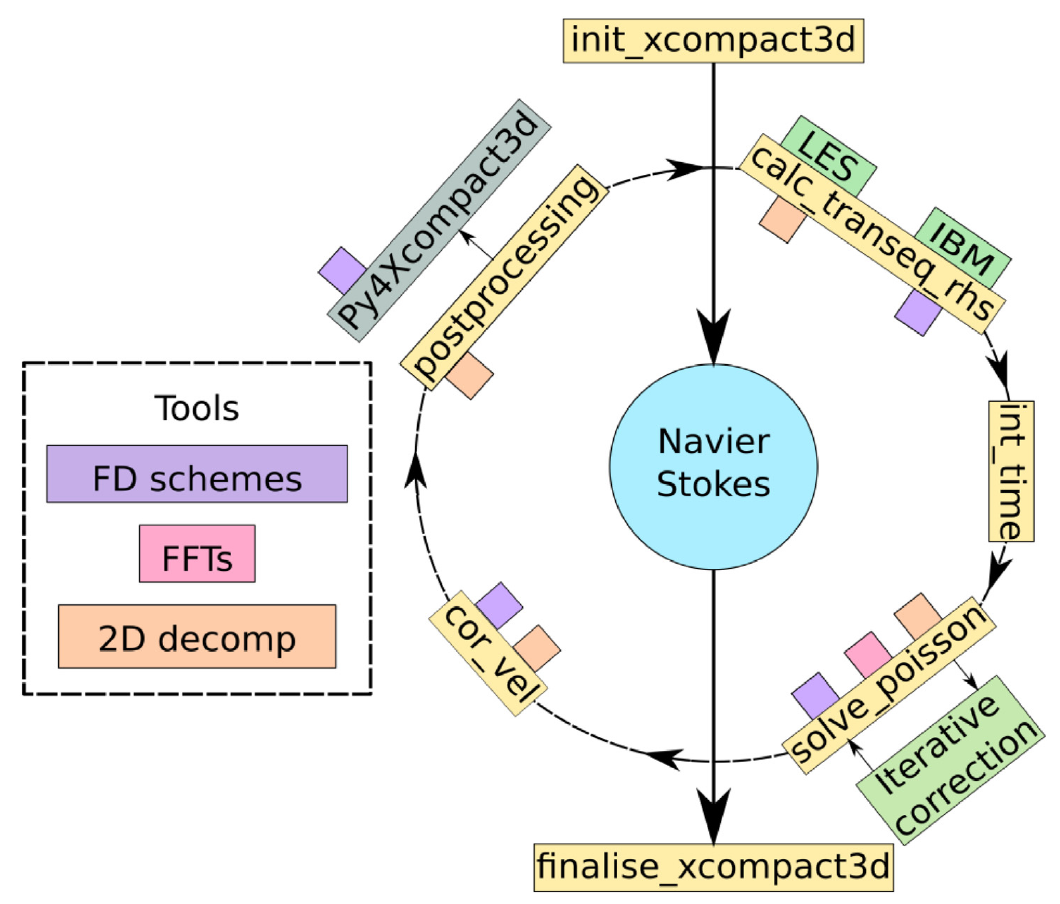
\includegraphics[width=0.49\textwidth]{figures/cap3/xc3d_architecture.png}
    	\label{fig:xc3d_archi}}  
    
    \subfloat[]{
    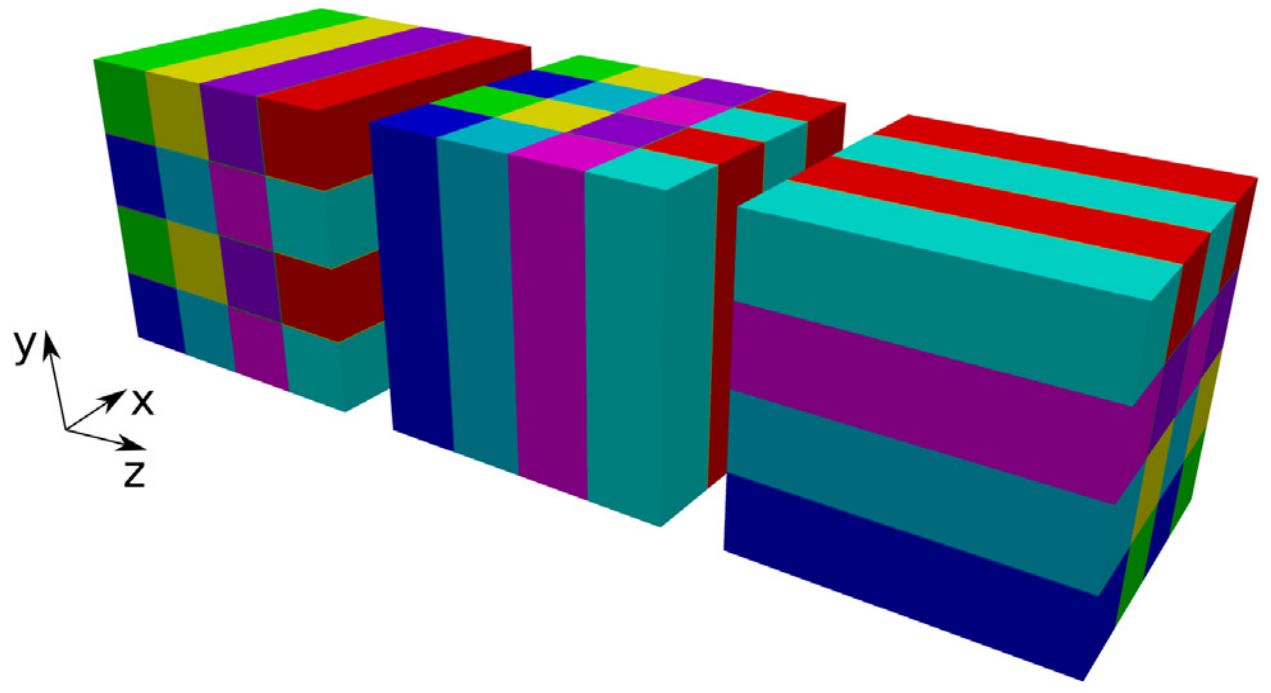
\includegraphics[width=0.49\textwidth]{figures/cap3/2d_decomp.png}
    	\label{fig:2d_decomp}}
 \caption{\textbf{(a)} Diagrama de la arquitectura de software de Xcompact3D. \textbf{(b)} Descomposición en lápices 2D utilizando 4 $\times$ 4 procesadores, representando los mismos en direcciones X, Y y Z respectivamente. Imágenes tomadas de \cite{bartholomew2020xcompact3d}.} 
 \label{fig:xc3d}
\end{figure}

El objetivo de las próximas subsecciones es ofrecer al lector una visión general de la lógica algorítmica de la herramienta numérica; se trata de un esquema conceptual a grandes rasgos, no de una descripción formal y rigurosa.

\subsection{Ecuaciones de gobierno}

Xcompact3D resuelve numéricamente las ecuaciones de Navier-Stokes para flujo incompresible junto con la ecuación de transporte de temperatura, acopladas entre sí mediante el término de fuerza boyante en la ecuación de momento. Las ecuaciones se expresan en forma adimensional en \ref{eq:sistem2} donde se omiten los superíndices ``*'' a fin de simplificar la notación. Obsérvese que si bien las ecuaciones están en consonancia con lo expuesto en el Capítulo \ref{cap:modelo}, no son exactamente las mismas. No obstante, estas ligeras diferencias no resultan relevantes en la explicación del método numérico.

\begin{equation}
\begin{aligned}
&\nabla \cdot \mathbf{u} = 0 \\
& \frac{\partial \mathbf{u}}{\partial t} = -\nabla \text{p} \underbrace{- (\mathbf{u} \cdot \nabla)\mathbf{u} + \frac{1}{\text{Re}} \nabla^2 \mathbf{u} + \mathbb{A} \hspace{0.5mm} \theta \hspace{0.5mm} \mathbf{e}_g + \mathbf{f} }_{\textbf{RHS}_{1}} \\
& \frac{\partial \theta}{\partial t} = \underbrace{- \mathbf{u} \cdot \nabla \theta + \frac{1}{\text{Re} \text{Pr}} \nabla^2 \theta + \mathbb{B} \hspace{0.5mm} u_x }_{\textbf{RHS}_2} \\
\end{aligned}
\label{eq:sistem2}
\end{equation}
En las ecuaciones precedentes: $\text{p}(\mathbf{x},t)$ es el campo de presiones; $\mathbf{u}(\mathbf{x},t)$ el campo de velocidades; $\theta(\mathbf{x},t)$ es el campo de temperatura; $\mathbf{x} = (x,y,z)$ es el vector de coordenadas y $t$ el tiempo; Re y Pr son los números adimensionales de Reynolds y Prandtl respectivamente; $\mathbb{A}$ y $\mathbb{B}$ son constantes que dependiendo de la forma adimensional considerada pueden ser diferentes, por ejemplo, tomando $\mathbb{A}=\text{Ri} / (\text{Re} \hspace{0.5mm} \text{Pr})$ y $\mathbb{B}=1$  se obtiene la forma adimensional de las ecuaciones \ref{eq:gob_system_adim}. La fuerza volumétrica $\mathbf{f}(\mathbf{x},t)$ es usado cuando se sumerge un cuerpo sólido dentro del dominio computacional (\textit{Immersed Boundary Method} \cite{peskin2002immersed}) o para otros usos según sea requerido.


\subsection{Esquemas de diferencias finitas de alto orden}

Las ventajas de los esquemas de alto orden para DNS/LES frente a los esquemas convencionales de bajo orden están plenamente reconocidas actualmente, especialmente por su capacidad de capturar con precisión un rango más amplio de escalas turbulentas para una resolución espacial dada. Los métodos espectrales estándar basados en representaciones de Fourier o de Chebyshev proporcionan soluciones muy precisas y eficientes de las ecuaciones de Navier-Stokes, aunque con severas restricciones en su aplicabilidad. Por su parte, los esquemas compactos de diferencias finitas de alto orden se aproximan a la precisión de los métodos espectrales y permiten mayor flexibilidad en la selección de condiciones de contorno (en XC3D es posible usar condiciones periódicas, de Dirichlet y de Neumann). Aunque los esquemas compactos son implícitos en el espacio, resultan muy competitivos en términos de eficiencia computacional. En particular, nuestras simulaciones emplean esquemas compactos de sexto orden para la discretización de los términos convectivo y difusivo.

\subsection{Avance temporal} \label{sec:time-ava}

El campo de flujo y el campo escalar se inicializan ya sea con una condición inicial (\texttt{init\_xcompact3d} en la Figura \ref{fig:xc3d_archi}) o cargando un archivo \textit{restart}. Las ecuaciones de Navier-Stokes se avanzan en el tiempo mediante un método de paso fraccionado (o proyección) implementado en tres etapas lógicas: (i) evaluación del lado derecho y \textit{predictor}, (ii) resolución de la ecuación de Poisson para la presión  e imposición de incompresibilidad y (iii) corrección de la velocidad y la temperatura.  En la Figura \ref{fig:xc3d_archi} se presenta una visión general de la arquitectura modular de \textit{Xcompact3D} \cite{bartholomew2020xcompact3d}. Las principales funcionalidades se separan en los modulos: \texttt{calc\_transeq\_rhs}, \texttt{int\_time}, \texttt{solve\_poisson}, \texttt{cor\_vel} y \texttt{postprocessing}. Los tres primeros corresponden a la resolución de las ecuaciones de gobierno, mientras que el último corresponde a la etapa de postprocesamiento de los datos obtenidos:


\begin{enumerate}
\item[\textbf{I}] \texttt{calc$\_$transeq$\_$rhs} $\rightarrow$ \texttt{int$\_$time}: predictor $\mathbf{u}^{\dagger \dagger}$ \\
Primero, se evalúan numéricamente los términos del lado derecho (\textbf{RHS}$_1$) de la ecuación de momento y se integran en el tiempo (una vez discretizados en el espacio) empleando, por ejemplo, esquemas de Runge-Kutta o Adams-Bashforth para obtener la velocidad intermedia $\mathbf{u}^{\dagger}$:

\begin{equation}
\frac{\mathbf{u}^{\dagger} - \mathbf{u}^k}{\Delta t} = \textbf{RHS}_1^k - c_k \nabla \widetilde{\text{p}}^k , 
\end{equation}
donde $c_k$ es un coeficiente conocido y $k$ el índice para los subpasos de tiempo \linebreak $k=1,...,n_k$; con $t_1=t_n$ y $t_{n_k}=t_{n+1}$ ($\Delta t = t_{n+1} - t_{n}$). La presión se expresa como su valor promediado en el tiempo en un subpaso dado ($c_k \Delta t$) indicado con una tilde $\widetilde{(\text{.})}$. Por conveniencia algebraica y para limpiar el lado derecho de la ecuación de Poisson de los pasos posteriores, puede definirse un campo intermedio $\mathbf{u}^{\dagger \dagger}$ que ``remueve'' la presión promedio usada en el predictor:

\begin{equation}
\frac{\mathbf{u}^{\dagger \dagger} - \mathbf{u}^{\dagger}}{\Delta t} = c_k \nabla \widetilde{\text{p}}^k  
\end{equation}
Con esta reordenación, $\mathbf{u}^{\dagger \dagger}$ sólo contiene los aportes no asociados a la presión previa:

\begin{equation}
\frac{\mathbf{u}^{\dagger \dagger} - \mathbf{u}^{k}}{\Delta t} = \textbf{RHS}_1^k \text{.}  
\end{equation}

\item[\textbf{II}] \texttt{solve\_poisson}: presión de proyección $\widetilde{p}^{k+1}$ \\
Se impone la incompresibilidad al final del paso:
	
\begin{equation}
\nabla \cdot \mathbf{u}^{k+1} = 0.
\label{eq:incomp}
\end{equation}
Tomando la divergencia de la corrección (véase ecuación \ref{eq:correccion}) y utilizando la ecuación \ref{eq:incomp}, se obtiene la ecuación de Poisson para la presión de proyección:

\begin{equation}
\nabla^2 \widetilde{\text{p}}^{k+1} = \frac{1}{c_k \Delta t} \nabla \cdot \mathbf{u}^{\dagger \dagger},
\end{equation}
donde $\widetilde{\text{p}}^{k+1}= \frac{1}{c_k \Delta t} \int^{t_{k+1}}_{t_k} \text{p} \hspace{0.5mm} dt$. 

Para la presión se aplican típicamente condiciones de borde de Neumann homogéneas (compatibles con la proyección). Por otro lado, las condiciones en la velocidad (por ejemplo, no deslizamiento) se aplican al predictor.

	\item[\textbf{III}]  \texttt{cor\_vel}: corrección solenoidal $\mathbf{u}^{k+1}$ \\
	Finalmente, se corrige la velocidad intermedia con el gradiente de la nueva presión para obtener
el campo solenoidal al final del paso de tiempo:

\begin{equation}
\frac{ \mathbf{u}^{k+1} - \mathbf{u}^{\dagger \dagger} }{\Delta t} = - c_k \nabla \widetilde{\text{p}}^{k+1} \text{.}
\label{eq:correccion}
\end{equation}

El término de la fuerza boyante no modifica la forma de la ecuación Poisson, sólo influye a través del predictor $\mathbf{u}^{\dagger \dagger}$ que genera. Adicionalmente, en el paso de tiempo actual $k$, se evalúa el lado derecho de la ecuación de transporte del escalar (\textbf{RHS}$_2$) empleando la velocidad del paso $k+1$, esto es:

\begin{equation}
\begin{aligned}
& \textbf{RHS}_2^k = - \mathbf{u}^{k+1} \cdot \nabla \theta^k + \frac{1}{\text{Re} \text{Pr}} \nabla^2 \theta^k + \mathbb{B} \hspace{0.5mm} u_x^{k+1}, \\
& \frac{\theta^{k+1} - \theta^{k}}{\Delta t} = \textbf{RHS}_2^k \text{.}
\end{aligned}
\end{equation}
Para la integración temporal de \textbf{RHS}$_2$ se emplea el mismo esquema utilizado en \textbf{RHS}$_1$.

\item[\textbf{IV}] \texttt{postprocessing} \\
Al final de cada paso de tiempo, el usuario puede decidir qué magnitudes almacenar y que cantidades calcular (magnitudes estadísticas de primer orden, segundo orden, etc).

\end{enumerate}

En particular, en este trabajo, para la integración temporal de los términos \textbf{RHS}$_{1,2}$ se emplea el esquema Adams-Bashforth de orden 3.



\subsection{\textit{Solver} espectral de Poisson}

Como se menciona en la Sección \ref{sec:time-ava}, Xcompact3D avanza las ecuaciones de gobierno mediante el método de paso fraccionario, formando una ecuación de Poisson para la presión al tomar la divergencia de la ecuación de momento. Una de las principales originalidades de Xcompact3D es que la ecuación de Poisson se resuelve en el espacio espectral usando el concepto de números de onda modificados \cite{lele1992compact}, para los cuales las operaciones en el espacio físico son estrictamente equivalentes a las del espacio espectral. Esta estrategia directa, que evita el uso de costosas técnicas iterativas, no es nueva para condiciones de contorno periódicas y/o de deslizamiento libre del campo de velocidades \cite{schumann1976direct}; asimismo, ha sido implementada y validada para condiciones de Dirichlet combinadas con esquemas de diferencias finitas de alto orden \cite{laizet2009high}.

\subsection{Biblioteca \textit{2D Decomp $\&$ FFT}}

Los esquemas de diferencias finitas y el \textit{solver} espectral de Poisson empleados por Xcompact3D se descomponen de forma natural en una serie de subproblemas unidimensionales. Por ello, resulta natural paralelizar el dominio computacional mediante una descomposición en “lápices”, como se ilustra en la Figura \ref{fig:2d_decomp}. Cada descomposición (en los ejes X, Y y Z, respectivamente) permite el cálculo independiente de derivadas, interpolaciones, etc. Las transposiciones globales para pasar de un lápiz a otro se realizan con comandos MPI. Más detalles sobre la estrategia de cómputo paralelo implementada en Xcompact3D pueden encontrarse en \cite{laizet2011incompact3d}.



\section{Orr-Somerfeld \textit{Mixed Convection} (OSMC)}

En el Capítulo \ref{cap:modelo}, empleando teoría de estabilidad lineal, considerando flujos laminares, y suponiendo las perturbaciones como ondas planas 3D (expresiones tipo \ref{eq:waves3d}) se arribó a un problema de autovalores y autofunciones generalizado, dado por la expresión \ref{eq:eigensistem-general}, con las condiciones de borde de la relación \ref{eq:eigensis-ci}. La herramienta numérica empleada para resolver este tipo de problemas es OSMC (por sus siglas, Orr-Somerfeld \textit{Mixed Convection}), desarrollada por Pablo Szuban como parte de su Proyecto Integrador de Ingeniería en el Instituto Balseiro \cite{szuban2023}. La herramienta numérica se implementó en lenguaje \textit{Python} utilizando las librerias \textit{NumPy} y \textit{SciPy}. La misma se encuentra disponible en GitHub: \href{https://github.com/Pato4184/OSMC-Repository}{OSMC-Repository}.

A continuación se dan los lineamientos detrás de la estrategia numérica utilizada. OSMC emplea el método numérico espectral conocido como ``Método de Colocación de la Matriz de Chebyshev'' \cite{moin2010fundamentals}. Esta estrategia busca transformar el problema de autovalores y autofunciones a uno de autovalores y autovectores. Los vectores solución son las amplitudes $\widehat{v_y}$, $\widehat{\varphi}$ y $\widehat{\eta}$ correspondientes a la frecuencia angular $\omega$ (autovalor asociado). Dado el sistema \ref{eq:eigensistem-general}, el flujo base laminar (Sección \ref{sec:fbase}) y las condiciones de borde asociadas, se discretiza la variable $y$ en el intervalo $\left[-1,1\right]$ en $N+1$ puntos de Chebyshev dados por la relación \ref{eq:cheb-points}. Lo siguiente es evaluar a las funciones involucradas en dichos puntos, por ejemplo, para una función arbitraria $\xi$ se tiene los puntos $\xi_j = \xi(y_j)$; luego, se construye un polinomio interpolante de Lagrange $\mathcal{L}$ para $\xi$ , de grado $\leq N$, tal que $\mathcal{L}(y_j) = \xi_j$.

\begin{equation}
y_j = \cos \left( \frac{j \hspace{0.5mm} \pi}{N} \right), \quad j=0,1,...,N 
\label{eq:cheb-points}
\end{equation}

De esta manera, los valores de la derivada de $\xi$ en los puntos $y_j$ son equivalentes a aquellos valores de la derivada del polinomio interpolante en los mismos puntos. Si $\xi$ se transforma a un vector\footnote{Es decir, los elementos $\xi_j$ del vector $\vec{\xi}$ son tales que $\xi_j = \xi(y_j)$.} $\vec{\xi}$, entonces, se puede demostrar \cite{moin2010fundamentals}, que la derivada de la función evaluada en los puntos de Chebyshev es $\vec{\xi^{\prime}} = \mathbb{D} \hspace{0.4mm} \vec{\xi}$ donde $\mathbb{D}$ es la Matriz de Colocación de Chebyshev de tamaño $(N+1) \times (N+1)$ \cite{trefethen}.

Si se tiene en cuenta que se necesita resolver un problema con condiciones de borde nulas (relaciones  \ref{eq:eigensis-ci}), es posible mostrar \cite{szuban2023}, que las primeras y últimas filas y columnas de la matriz $\mathbb{D}$ se pueden eliminar  de modo que resulta una matriz de $(N-1) \times (N-1)$ . Siguiendo este concepto, es posible obtener los operadores de derivada primera, segunda y cuarta, necesarios para la resolución del problema. Finalmente, al considerar todo lo explicitado, se obtiene un problema de autovalores y autovectores (generalizado) de matrices de tamaño  $3(N-1) \times 3(N-1)$ como se muestra en la expresión \ref{eq:eigensistem-matrix}. 

\begin{equation}
\begin{bmatrix}
A_{11} & A_{12} & \mathbb{O} \\[4pt]
A_{21} & A_{22} & A_{23} \\[4pt]
A_{31} & A_{32} & A_{33}
\end{bmatrix}
\,\begin{bmatrix}
\vec{\widehat{v_y} } \\[4pt]
\vec{\widehat{\varphi}} \\[4pt]
\vec{\widehat{\eta}}
\end{bmatrix}
\;=\; i \omega
\,\begin{bmatrix}
  B_1 & \mathbb{O} & \mathbb{O} \\[4pt]
    \mathbb{O} & \mathbb{I} & 0 \\[4pt]
    \mathbb{O} & \mathbb{O} & \mathbb{I}
\end{bmatrix}
\,\begin{bmatrix}
\vec{\widehat{v_y}} \\[4pt]
\vec{\widehat{\varphi}} \\[4pt]
\vec{\widehat{\eta}}
\end{bmatrix}
\label{eq:eigensistem-matrix}
\end{equation}

\begin{align*}
A_{11} &= \frac{1}{\text{Re}_b} \left[ \mathbb{D}^2 - k^2 \mathbb{I} \right]^2 - i \alpha \left( \mathtt{diag}(\vec{V_x}) ( \mathbb{D}^2 - k^2 \mathbb{I})  + \mathtt{diag}(\mathbb{D}^2 \vec{V_x}) \right) \hspace{2mm} ; \hspace{2mm} A_{12} = -\left[ i \alpha \frac{\text{Ra}}{\text{Re}_b} \mathbb{D} \right] \\ 
A_{21} &= \frac{i \alpha}{\text{Re}_b \hspace{1mm} \text{Pr} \hspace{1mm} k^2} \mathbb{D} + \mathtt{diag}(\mathbb{D}\vec{\Phi}) \hspace{2mm} ; \hspace{2mm} A_{22} = \frac{-1}{\text{Re}_b \hspace{1mm} \text{Pr} } \left[ \mathbb{D}^2 - k^2 \mathbb{I} \right] + i \alpha \hspace{0.4mm} \mathtt{diag}(\vec{V_x})  \hspace{2mm} ; \hspace{2mm} A_{23} = \frac{\beta}{\text{Re}_b \hspace{1mm} \text{Pr} \hspace{1mm} k^2} \mathbb{I} \\
A_{31} &= \beta \hspace{0.4mm} \mathtt{diag}(\mathbb{D} \vec{V_x}) \hspace{2mm} ; \hspace{2mm} A_{32} = - \beta \frac{\text{Ra}}{\text{Re}_b} \mathbb{I}   \hspace{2mm} ; \hspace{2mm} A_{33} = -\frac{1}{\text{Re}_b} \left[ \mathbb{D}^2 - k^2 \mathbb{I} \right] + i \alpha \hspace{0.4mm}  \mathtt{diag}(\vec{V_x}) \\
B_1    &= - \left[ \mathbb{D}^2 - k^2 \mathbb{I} \right] \hspace{2mm} ; \hspace{2mm} k^2 = \alpha^2 + \beta^2 \\
\end{align*}
Como puede observarse, las submatrices $A_{11}$, $A_{21}$, $A_{22}$, $A_{31}$ y $A_{33}$ tienen incorporado en su definición al operador $\mathtt{diag}$. El mismo transforma un vector $\vec{\xi}$, de tamaño $n \times 1$, en una matriz diagonal $n \times n$ cuyos elementos diagonales son los elementos de $\vec{\xi}$. Asimismo, $\mathbb{I}$ es la matriz identidad de tamaño $(N-1) \times (N-1)$ y $\mathbb{O}$ es la matriz nula de igual tamaño.

\chapter{Validación de Herramientas Numéricas} \label{cap:validacion}


En este capítulo se pretende validar y asegurar el correcto funcionamiento de las \linebreak herramientas numéricas utilizadas. El mismo se divide en dos partes. Una primera parte que se centra en validar la herramienta de simulaciones DNS, Xcompact3D. Para tal fin se emplean diferentes mallas (o resoluciones) espaciales y pasos temporales según se requiera. En la segunda parte de este capítulo se valida la herramienta generadora de autovalores y autofunciones, OSMC. 

\textcolor{black}{Se emplean cuatro situaciones diferentes para validar XC3D: (i) un canal de placas\linebreak paralelas en régimen turbulento, donde se valida el comportamiento puramente hidrodinámico \cite{moser1999}; (ii) un canal turbulento hidrodinámica y térmicamente desarrollado con flujo de calor constante en las paredes, donde se analizan aspectos hidrodinámicos y térmicos para convección forzada \cite{kawamura2000dns}; (iii) mismo sistema físico que el caso anterior pero en régimen laminar, teniendo en cuenta el acople de las ecuaciones de conservación debido al término de fuerza boyante \cite{chen1996linear}; (iv) canal vertical de placas paralelas isotérmicas a distinta temperatura entre sí, en régimen  turbulento con convección mixta \cite{guo2022direct}. En los casos turbulentos se analiza la convergencia en malla y la opción computacionalmente más económica que satisfaga una precisión aceptable.}

La corroboración de la herramienta numérica OSMC se realiza en dos etapas: (i) se ratifica que OSMC genere los autovalores correctos, para eso se considera la variación de la parte \linebreak imaginaria del autovalor más inestable en función del número de onda \cite{chen1996linear}; (ii) se corrobora que las autofunciones entregadas por el código sean correctas y para ello se utiliza como referencia autofunciones asociadas a ondas 2D y 3D \cite{chen2003direct}.

Adicionalmente, las predicciones producidas por la teoría de estabilidad lineal, sobre la evolución temporal de ciertas magnitudes de interés, se comparan con aquellos resultados obtenidos vía simulaciones DNS. En general, se observa que las herramientas empleadas \linebreak responden adecuadamente y son consistentes con los datos de referencia.


\newpage
 
\section{Primera Parte: Xcompact3D}

En esta sección se presentan los resultados obtenidos con la herramienta numérica \linebreak Xcompact3D (XC3D) para un canal de placas paralelas en flujo completamente desarrollado. Para la validación de XC3D se consideran las siguientes situaciones de flujo: 

\begin{itemize}

\item \textbf{Situación I:} flujo turbulento hidrodinámico y completamente desarrollado,

\item \textbf{Situación II:} flujo turbulento hidrodinámica y térmicamente desarrollado con flujo de calor constante en las paredes, considerando únicamente convección forzada.

\item \textbf{Situación III:} flujo en régimen laminar hidrodinámica y térmicamente desarrollado con flujo de calor constante en las paredes donde se considera el efecto de la fuerza boyante, es decir, en régimen de convección mixta; 

\item \textbf{Situación IV:} por último, se considera un canal turbulento completamente desarrollado (hidrodinámica y térmicamente) con convección mixta cuyas paredes están sometidas a una diferencia de temperatura constante. 

\end{itemize}
En cada una de las situaciones expuestas, los resultados se comparan con datos de referencia.

A lo largo de la etapa de validación, para las distintas simulaciones DNS realizadas, se emplearon distintas resoluciones espaciales y pasos temporales, las cuales se especifican en la Tabla \ref{tab:meshes}. Asimismo, en dicha tabla se expresan la cantidad de nodos utilizados en las direcciones $X$, $Y$ y $Z$ (N$_x$, N$_y$ y N$_z$, respectivamente). Nótese, además, que la discretización empleada en la dirección $Y$ es no uniforme. El dominio utilizado en todas las simulaciones corresponde a L$_x \times$ L$_y \times$ L$_z$ = $8 \times 2 \times 4$.

Por otro lado, en cada simulación (según se requiera) se imponen los parámetros Re$_o$, Pr y/o Ri$_b$. Posteriormente, se deja evolucionar el sistema hasta que los campos asociados alcancen el estado estadísticamente estacionario. Una vez en dicho estado, se colecta estadística por al menos 500 unidades temporales. Para acelerar la obtención del estado turbulento, XC3D cuenta con la capacidad de introducir  ruido aleatorio, y/o también rotación\footnote{La rotación se logra agregando un término asociado a la fuerza de Coriolis en la ecuación de momento \cite{lamballais2014}, que viene implementada en el propio código.} en el propio flujo. 

Las simulaciones se realizan en el \textit{cluster ``mecclust''} del grupo MECOM (CAB-CNEA). Dependiendo de la disponibilidad y de la exigencia demandada, cada simulación se puede \linebreak correr en un nodo individual de los veinte disponibles, los cuales emplean 2 procesadores \textit{Xeon E5 2660 V3 @2.6 GHz} con 10 \textit{cores} cada uno; o también, si se requiere, es posible utilizar cuatro nodos con conexión \textit{InfiniBand} que da un total de 80 \textit{cores}. Para aquellas simulaciones más demandantes, se tiene $\sim 800$ pasos temporales por hora de reloj ($\sim 4\text{.}5 \text{ } seg/\text{paso}$), y el almacenamiento requerido puede alcanzar los 100 GB. Para dar una idea general del \textit{wall-clock} requerido, empleando 20 \textit{cores}, una simulación de 500 unidades temporales con la malla M0 (véase Tabla \ref{tab:meshes}) puede tardar del orden de 35 minutos mientras que una simulación idéntica con la malla M4 puede requerir del orden de 670 horas.       


\begin{table}[H]
\centering
\resizebox{0.75\textwidth}{!}{%
\begin{tabular}{lcccc}
\toprule
Nomenclatura & N$_x \times$ N$_y \times$ N$_z$ & $(\Delta x^*,\Delta y^*_{\text{min}},\Delta y^*_{\text{max}},\Delta z^*)$ & $\Delta t^*$ \\
\midrule
M0 & $64 \times 65 \times 64$    & (0.125, 0.011, 0.087, 0.062) & 0.005 \\
M1 & $128 \times 65 \times 64$   & (0.062, 0.011, 0.087, 0.062) & 0.005 \\
M2 & $128 \times 129 \times 128$ & (0.062, 0.006, 0.044, 0.031) & 0.002 \\
M3 & $160 \times 161 \times 160$ & (0.05,  0.004, 0.035, 0.025)  & 0.001 \\
M4 & $256 \times 257 \times 256$ & (0.031, 0.003, 0.022, 0.015)  & 0.001 \\
\bottomrule
\end{tabular}}
\caption{Distintas resoluciones espaciales y temporales utilizadas \textcolor{black}{(adimensionales)} en las simulaciones de validación. Debido a que la discretización en la dirección $Y$ es no uniforme, se reporta tanto el mínimo como el máximo $\Delta y$ asociado.}
\label{tab:meshes}
\end{table}

Algunos resultados, presentes en esta primera parte, se encuentran adimensionalizados en unidades de pared (indicadas con el superíndice ``+'') basadas en el semiancho del canal $d$, la velocidad de fricción $u_{\tau}$ y la temperatura de fricción $T_{\tau}$:

\begin{itemize}
	\item Esfuerzo de Corte: $\tau_w= \mu_o \partial u_x / \partial y$ (evaluada en $y=\pm d$)  
	\item $u_{\tau} = \sqrt{\tau_w / \rho}$ ; $T_{\tau}=\frac{q''_w}{\rho c_p u_{\tau}}$
	\item $\mathbf{u}^+ = \mathbf{u} / u_{\tau}$ ; $\theta^+ = \theta / T_{\tau}$ ; $y^+ = \frac{u_{\tau} y}{\nu_o}$
\end{itemize}
Por otro lado, los perfiles de las magnitudes seleccionadas se encuentran promediadas en la dirección X y Z, y en el tiempo.

\subsection{Situación I. Canal turbulento hidrodinámico}

%En esta subsección se exponen los resultados del canal turbulento considerando los \linebreak aspectos hidrodinámicos únicamente. Esto es, considerando el sistema mostrado en la Figura \ref{fig:sistem_domain} donde se considera en este caso particular, $q''_w=0$ En este caso se impone Re$_o$=4200 y se realizan \linebreak simulaciones para las mallas M0, M1, M2 y M3.  

\textcolor{black}{En esta subsección se presentan los resultados del canal turbulento considerando únicamente los aspectos hidrodinámicos. Es decir, se analiza el sistema mostrado en la Figura \ref{fig:sistem_domain}, donde en este caso particular se toma $q''_w = 0$. Para esta configuración, se fija Re$_o = 4200$ y se realizan simulaciones utilizando las mallas M0, M1, M2 y M3.}

En las Figuras \ref{fig:kim-ux} - \ref{fig:kim-uxuy} se presentan (respectivamente) algunas magnitudes de interés para este sistema: el perfil de velocidad \textit{streamwise} $\langle u^+_x \rangle$ y los perfiles de las componentes del tensor de Reynolds\footnote{Sea $R_{ij} = \langle u^{\prime}_i u^{\prime}_j \rangle$ el tensor de Reynolds, entonces: la raíz cuadrada de la componente diagonal $R_{ii}$ coincide con el valor rms de la fluctuación de velocidad en la dirección $i$-ésima. Esto es, $(u_i)_{rms} = \sqrt{R_{ii}}$.} $\sqrt{\langle u^{+ \prime}_x u^{+ \prime}_x \rangle}$, $\sqrt{\langle u^{+ \prime}_y u^{+ \prime}_y \rangle}$ y $\langle u^{+ \prime}_x u^{+ \prime}_y \rangle$. En estas gráficas se comparan las distintas mallas empleadas con el trabajo de Moser \textit{et al.} \cite{moser1999}. Al refinar la malla (M0$\rightarrow$M3), las cantidades de interés se estabilizan; entre M2 y M3 las diferencias son prácticamente despreciables. Por lo tanto, se considera alcanzada la independencia de malla. Con esa resolución, los resultados DNS de XC3D muestran buen acuerdo con los datos de referencia.

\newpage

\begin{figure}[H]
 \centering
    \subfloat[]{
    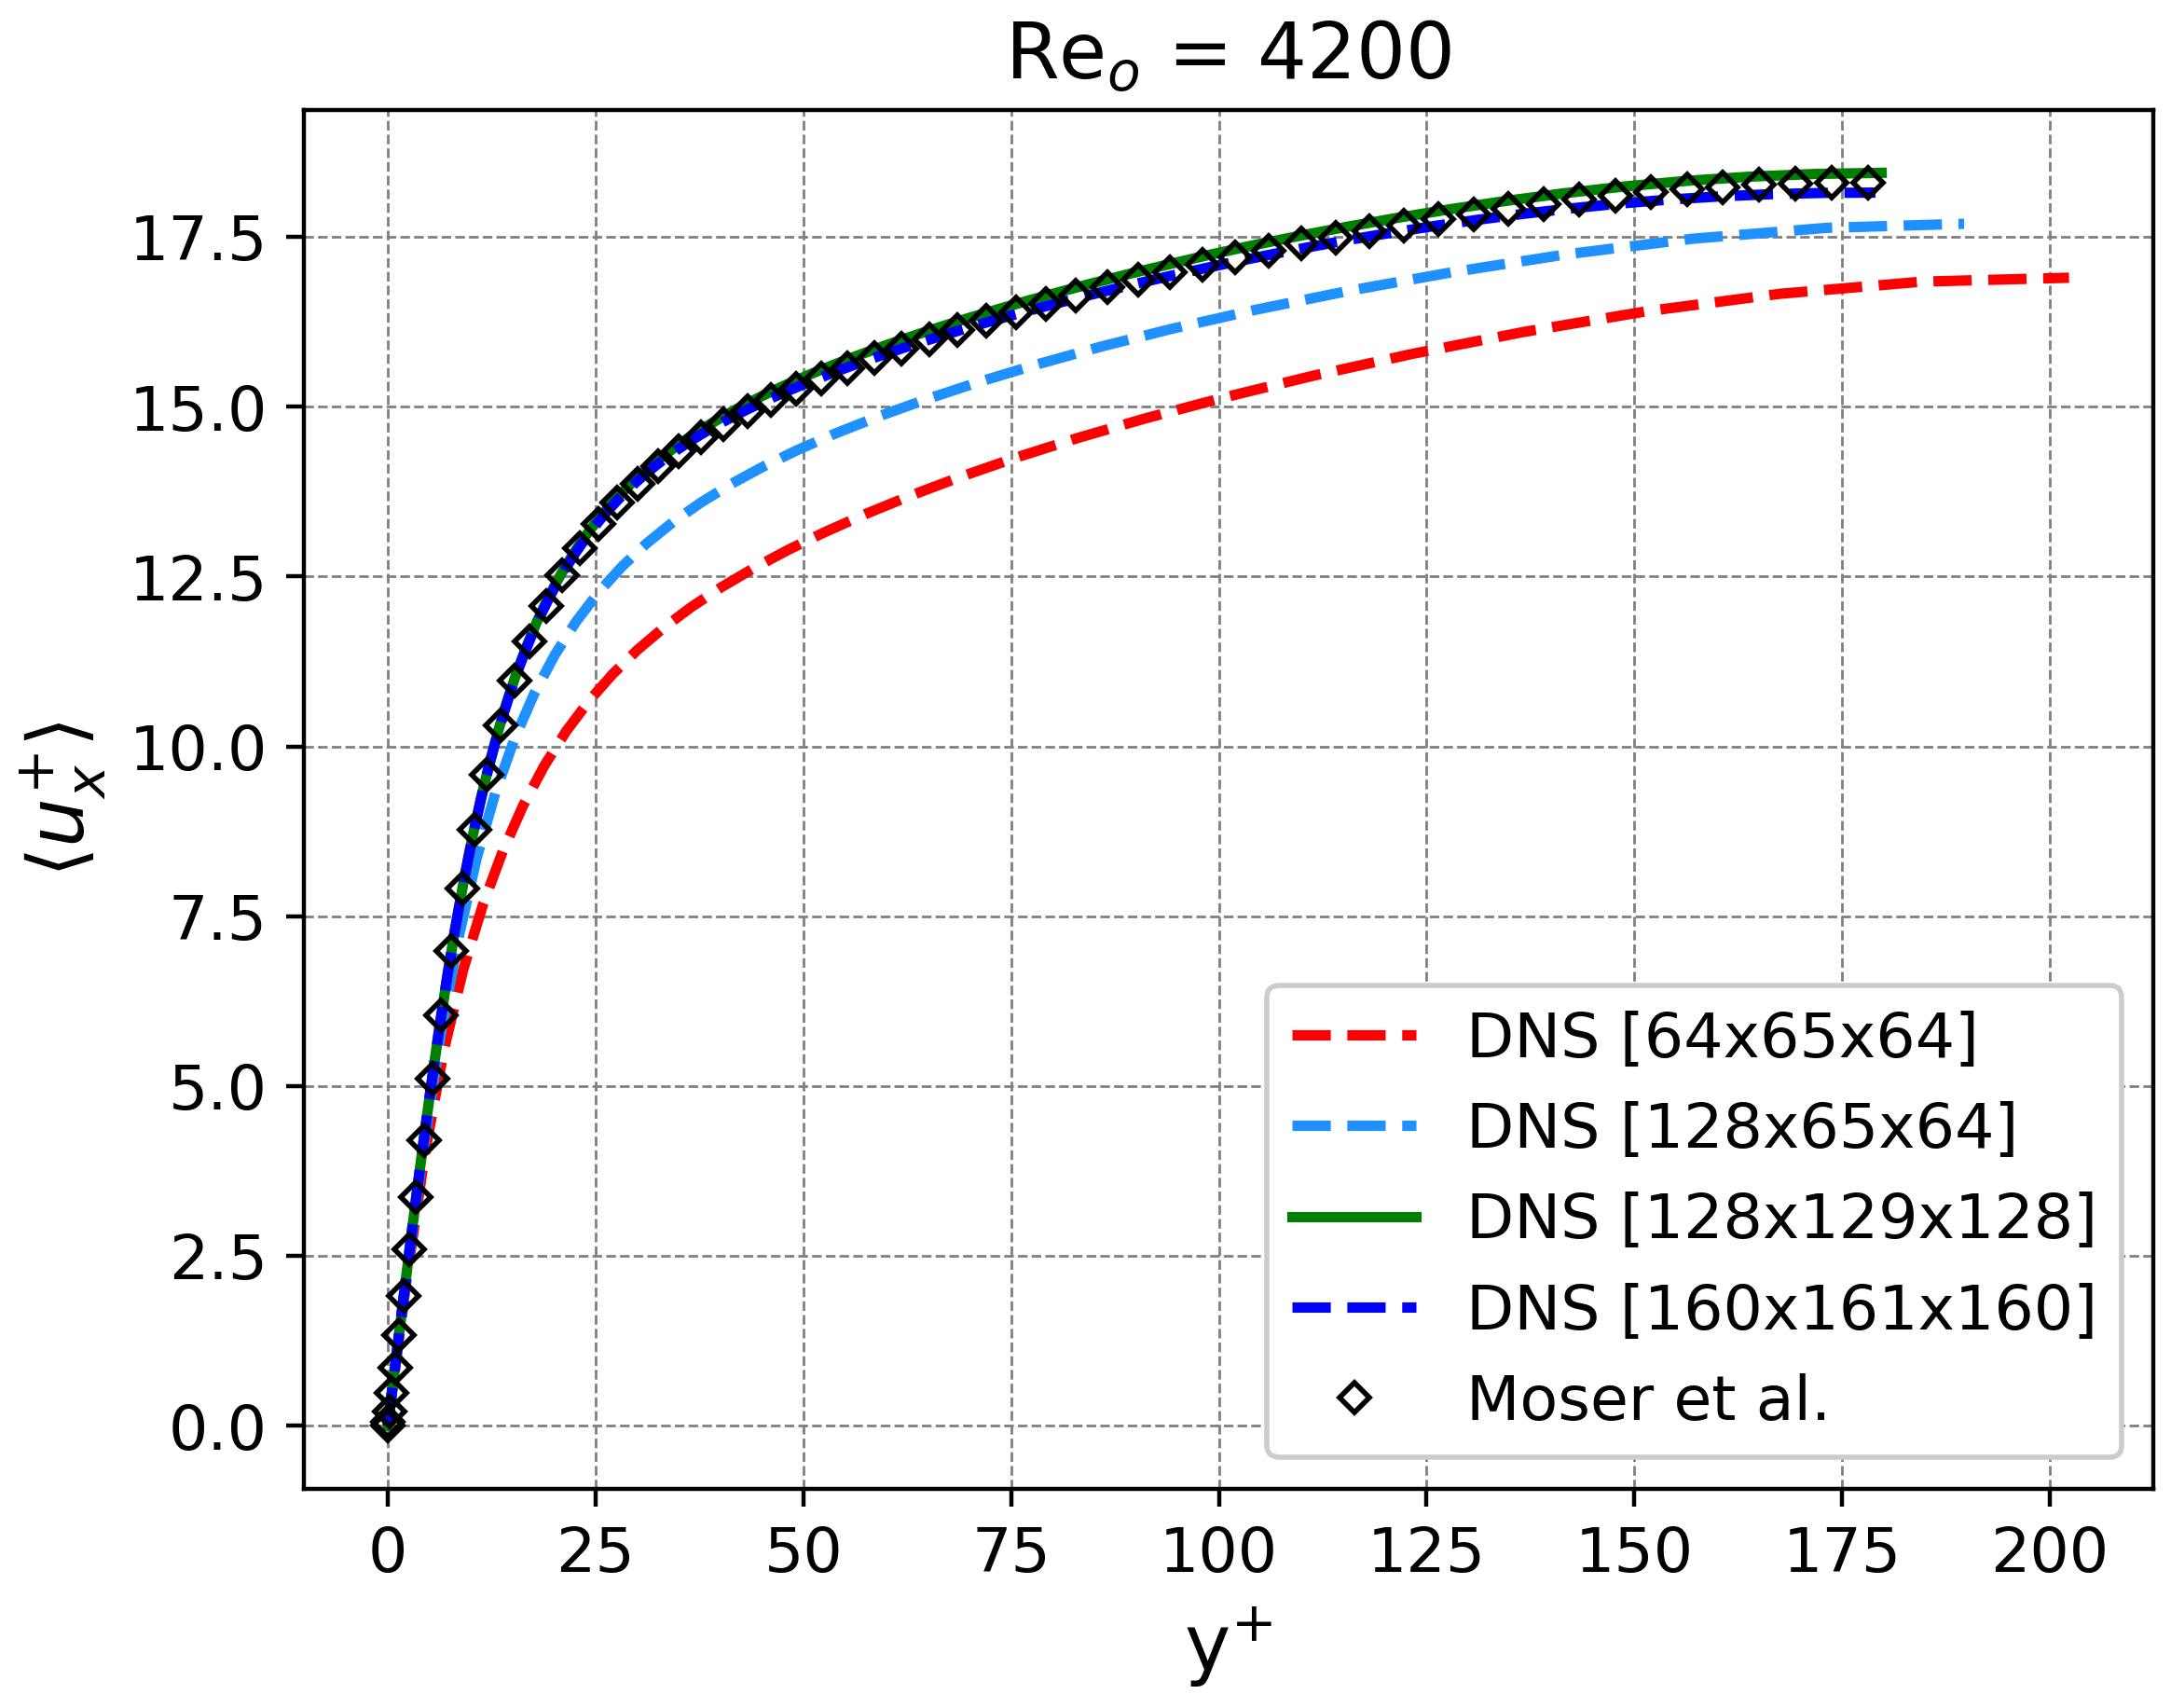
\includegraphics[width=0.49\textwidth]{figures/cap4/kim/ux_mean.png}
    	\label{fig:kim-ux}}  
    \subfloat[]{
    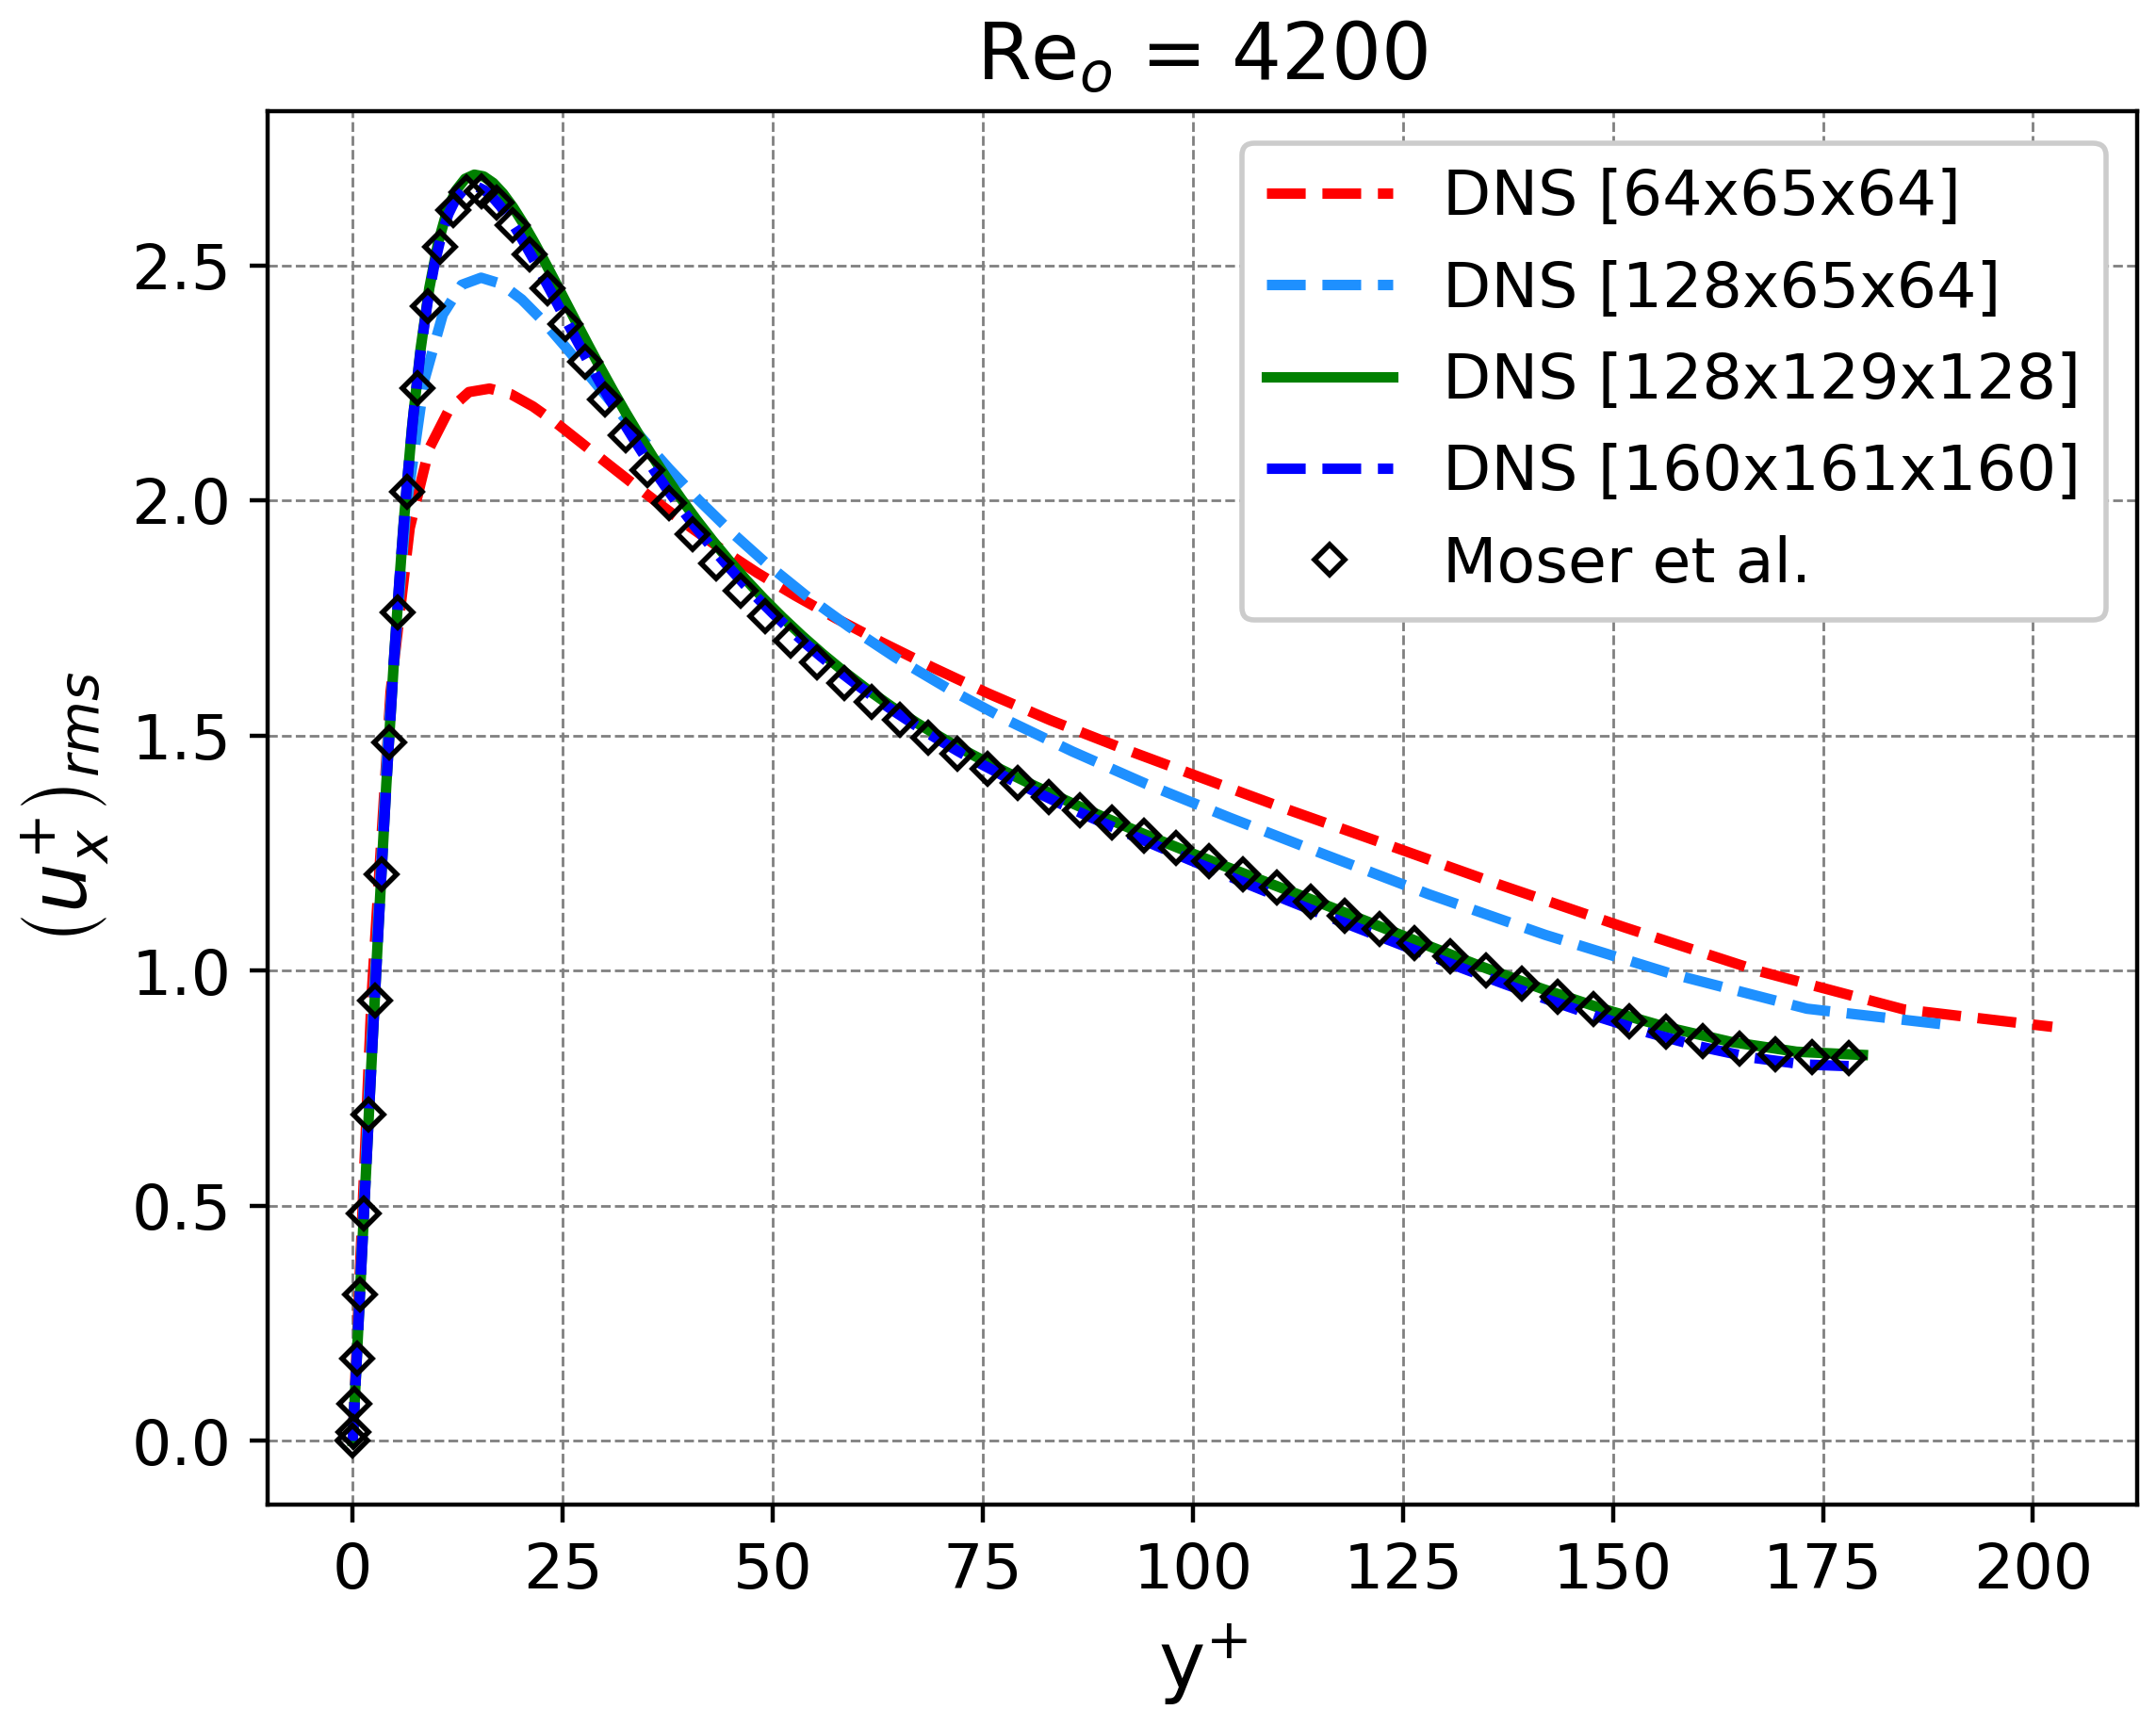
\includegraphics[width=0.49\textwidth]{figures/cap4/kim/ux_rms.png}
    	\label{fig:kim-ux-rms}}
    
    \subfloat[]{
    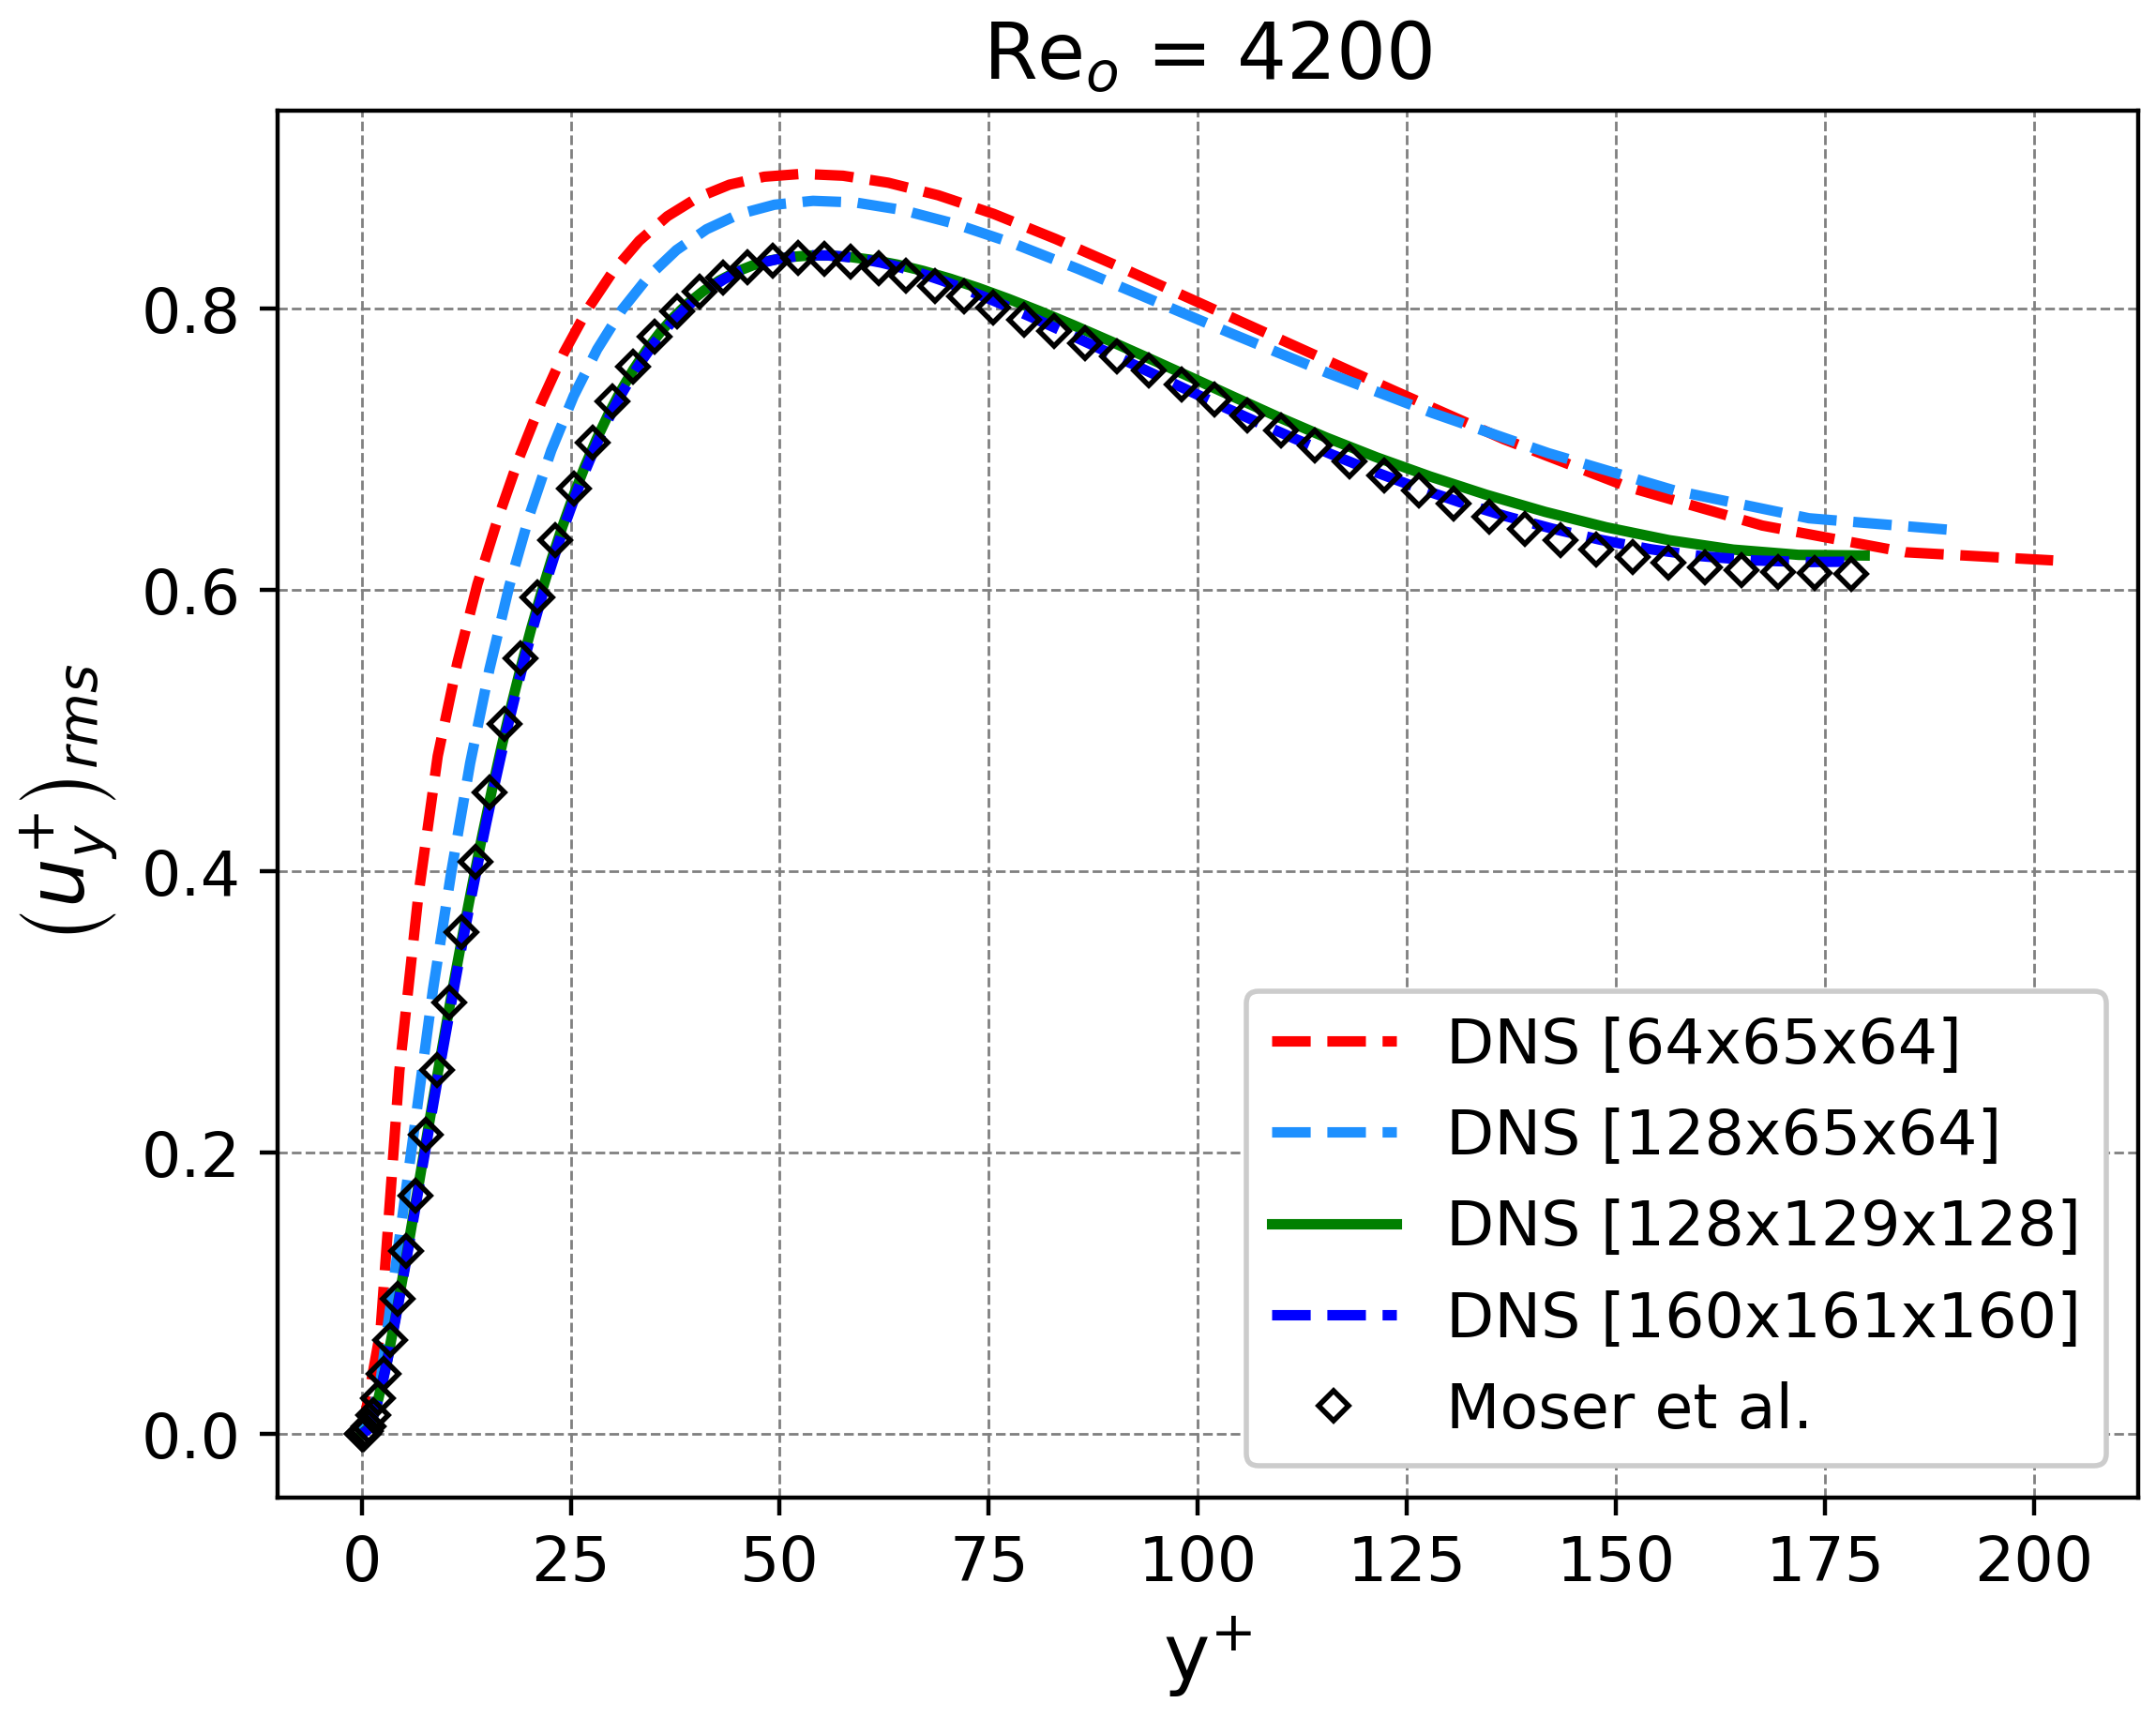
\includegraphics[width=0.49\textwidth]{figures/cap4/kim/uy_rms.png}
    	\label{fig:kim-uy}}  
    \subfloat[]{
    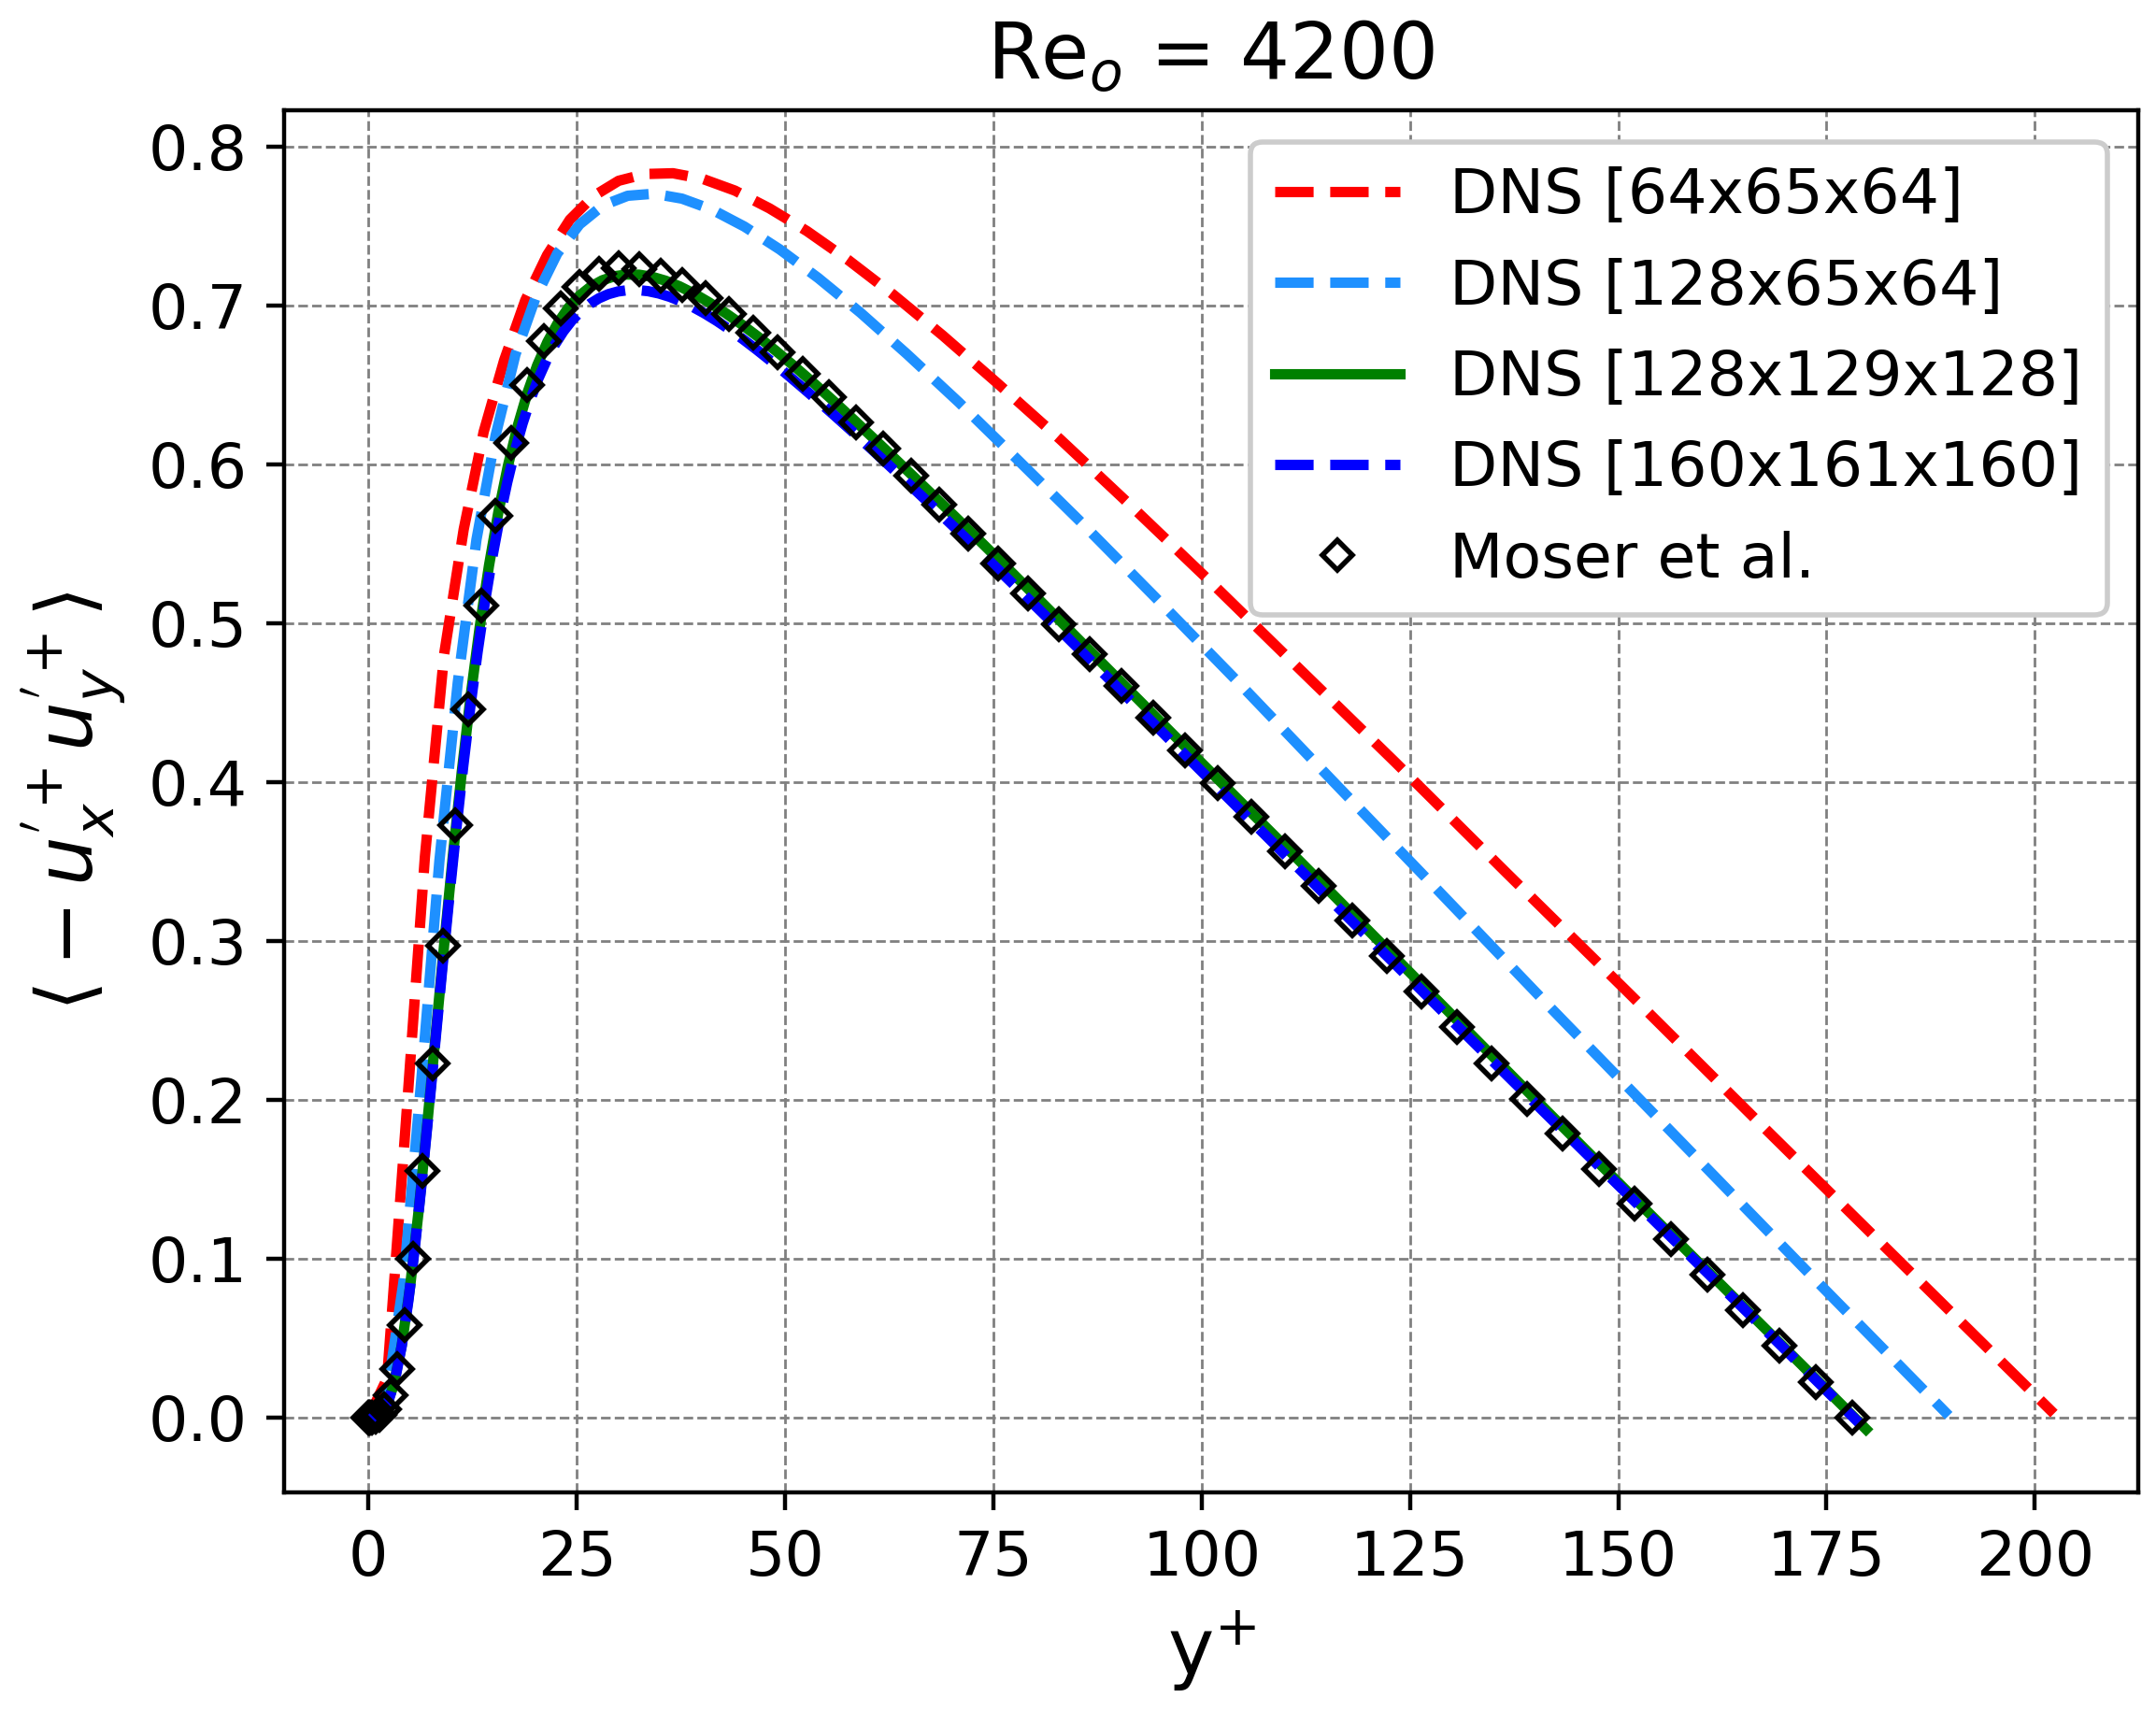
\includegraphics[width=0.49\textwidth]{figures/cap4/kim/up_vp.png}
    	\label{fig:kim-uxuy}} 
 \caption{Perfiles de \textbf{(a)} velocidad media \textit{streamwise}, \textbf{(b)} fluctuaciones RMS de la velocidad en $\langle u^+_x \rangle$, \textbf{(c)} fluctuaciones RMS de la velocidad $\langle u^+_y \rangle$ y \textbf{(d)} componente $xy$ del tensor de Reynolds. \textcolor{black}{Estos perfiles corresponden al sistema mostrado en la Figura \ref{fig:sistem_domain} ($q''_w=0$).}} 
 \label{fig:kim_1}
\end{figure}

\begin{table}[H]
\centering
\resizebox{0.9\textwidth}{!}{%
\begin{tabular}{lccccc}
\toprule
Nomenclatura & L$_x \times$ L$_y \times$ L$_z$ & N$_x \times$ N$_y \times$ N$_z$ & $(\Delta x^*,\Delta z^*)$ & $\Delta y^*_{\text{max}}$ \\
\midrule
A & $6\text{.}4d \times 2 \times 3\text{.}2d $ & $128 \times 66 \times 128$    & (0.05, 0.025) & 0.064 \\
C & $12\text{.}8d \times 2 \times 6\text{.}4d $ & $256 \times 128 \times 256$  & (0.05, 0.025) & 0.033 \\
D & $6\text{.}4d \times 2 \times 3\text{.}2d $ & $1024 \times 480 \times 512$   & (0.006, 0.006) & 0.0054 \\

\bottomrule
\end{tabular}}
\caption{Resoluciones espaciales empleadas por Kawamura \textit{et al.} \cite{kawamura2000dns}.}
\label{tab:meshes-kawa}
\end{table}

\newpage


\subsection{Situación II. Transporte de escalar pasivo en convección forzada con $q''_w$ constante}

En este caso se considera sólo el régimen de convección forzada, lo que equivale a suponer $\Pi=0$ en la ecuación de momento. De esta forma, las ecuaciones de continuidad y momento quedan desacopladas de la ecuación de energía (ecuaciones \ref{eq:gob_system_adim}). En este sentido, los campos solución de la velocidad son exactamente los mismos que en la \textbf{Situación I} y el campo de temperatura es un campo escalar que no interviene en el desarrollo hidrodinámico del sistema, sino únicamente en el aspecto térmico del flujo. Por ello, sólo se presentan magnitudes asociadas a la temperatura adimensional. Para las simulaciones asociadas a esta subsección, se considera el número de Reynolds Re$_o=4278$. 

\paragraph{Convergencia en Malla.}
En primer lugar, se analiza la respuesta del campo escalar solución frente a diferentes mallas, en concreto, se emplean aquellas mismas utilizadas en la \textbf{Situación I}.  Las Figuras \ref{fig:kmesh-theta} - \ref{fig:kmesh-uy-theta} presentan los perfiles de la temperatura adimensional, sus fluctuaciones y los flujos de calor turbulento en las direcciones X e Y, respectivamente. Las \linebreak simulaciones propias se comparan con aquellas obtenidas en la referencia \cite{kawamura2000dns} para Pr=0.71. Además, en dichas gráficas se exponen los distintos resultados obtenidos por Kawamura \textit{et al.} para diferentes mallas empleadas en su trabajo (véase Tabla \ref{tab:meshes-kawa}). 




De forma análoga al caso anterior, se observa claramente la convergencia con el refinamiento de malla: a medida que aumenta la resolución, los resultados se mantienen en buen acuerdo con las referencias. En particular, las curvas correspondientes a M2 y M3 no muestran diferencias apreciables a la escala de las figuras; en otras palabras, el paso de M2 a M3 no introduce mejoras perceptibles. En este sentido, se observa que la malla M2 (un compromiso adecuado entre precisión y costo computacional) reproduce con buen acuerdo los resultados de Moser \textit{et al.} \cite{moser1999} y Kawamura \textit{et al.} \cite{kawamura2000dns}.

\newpage

\begin{figure}[H]
 \centering
    \subfloat[]{
    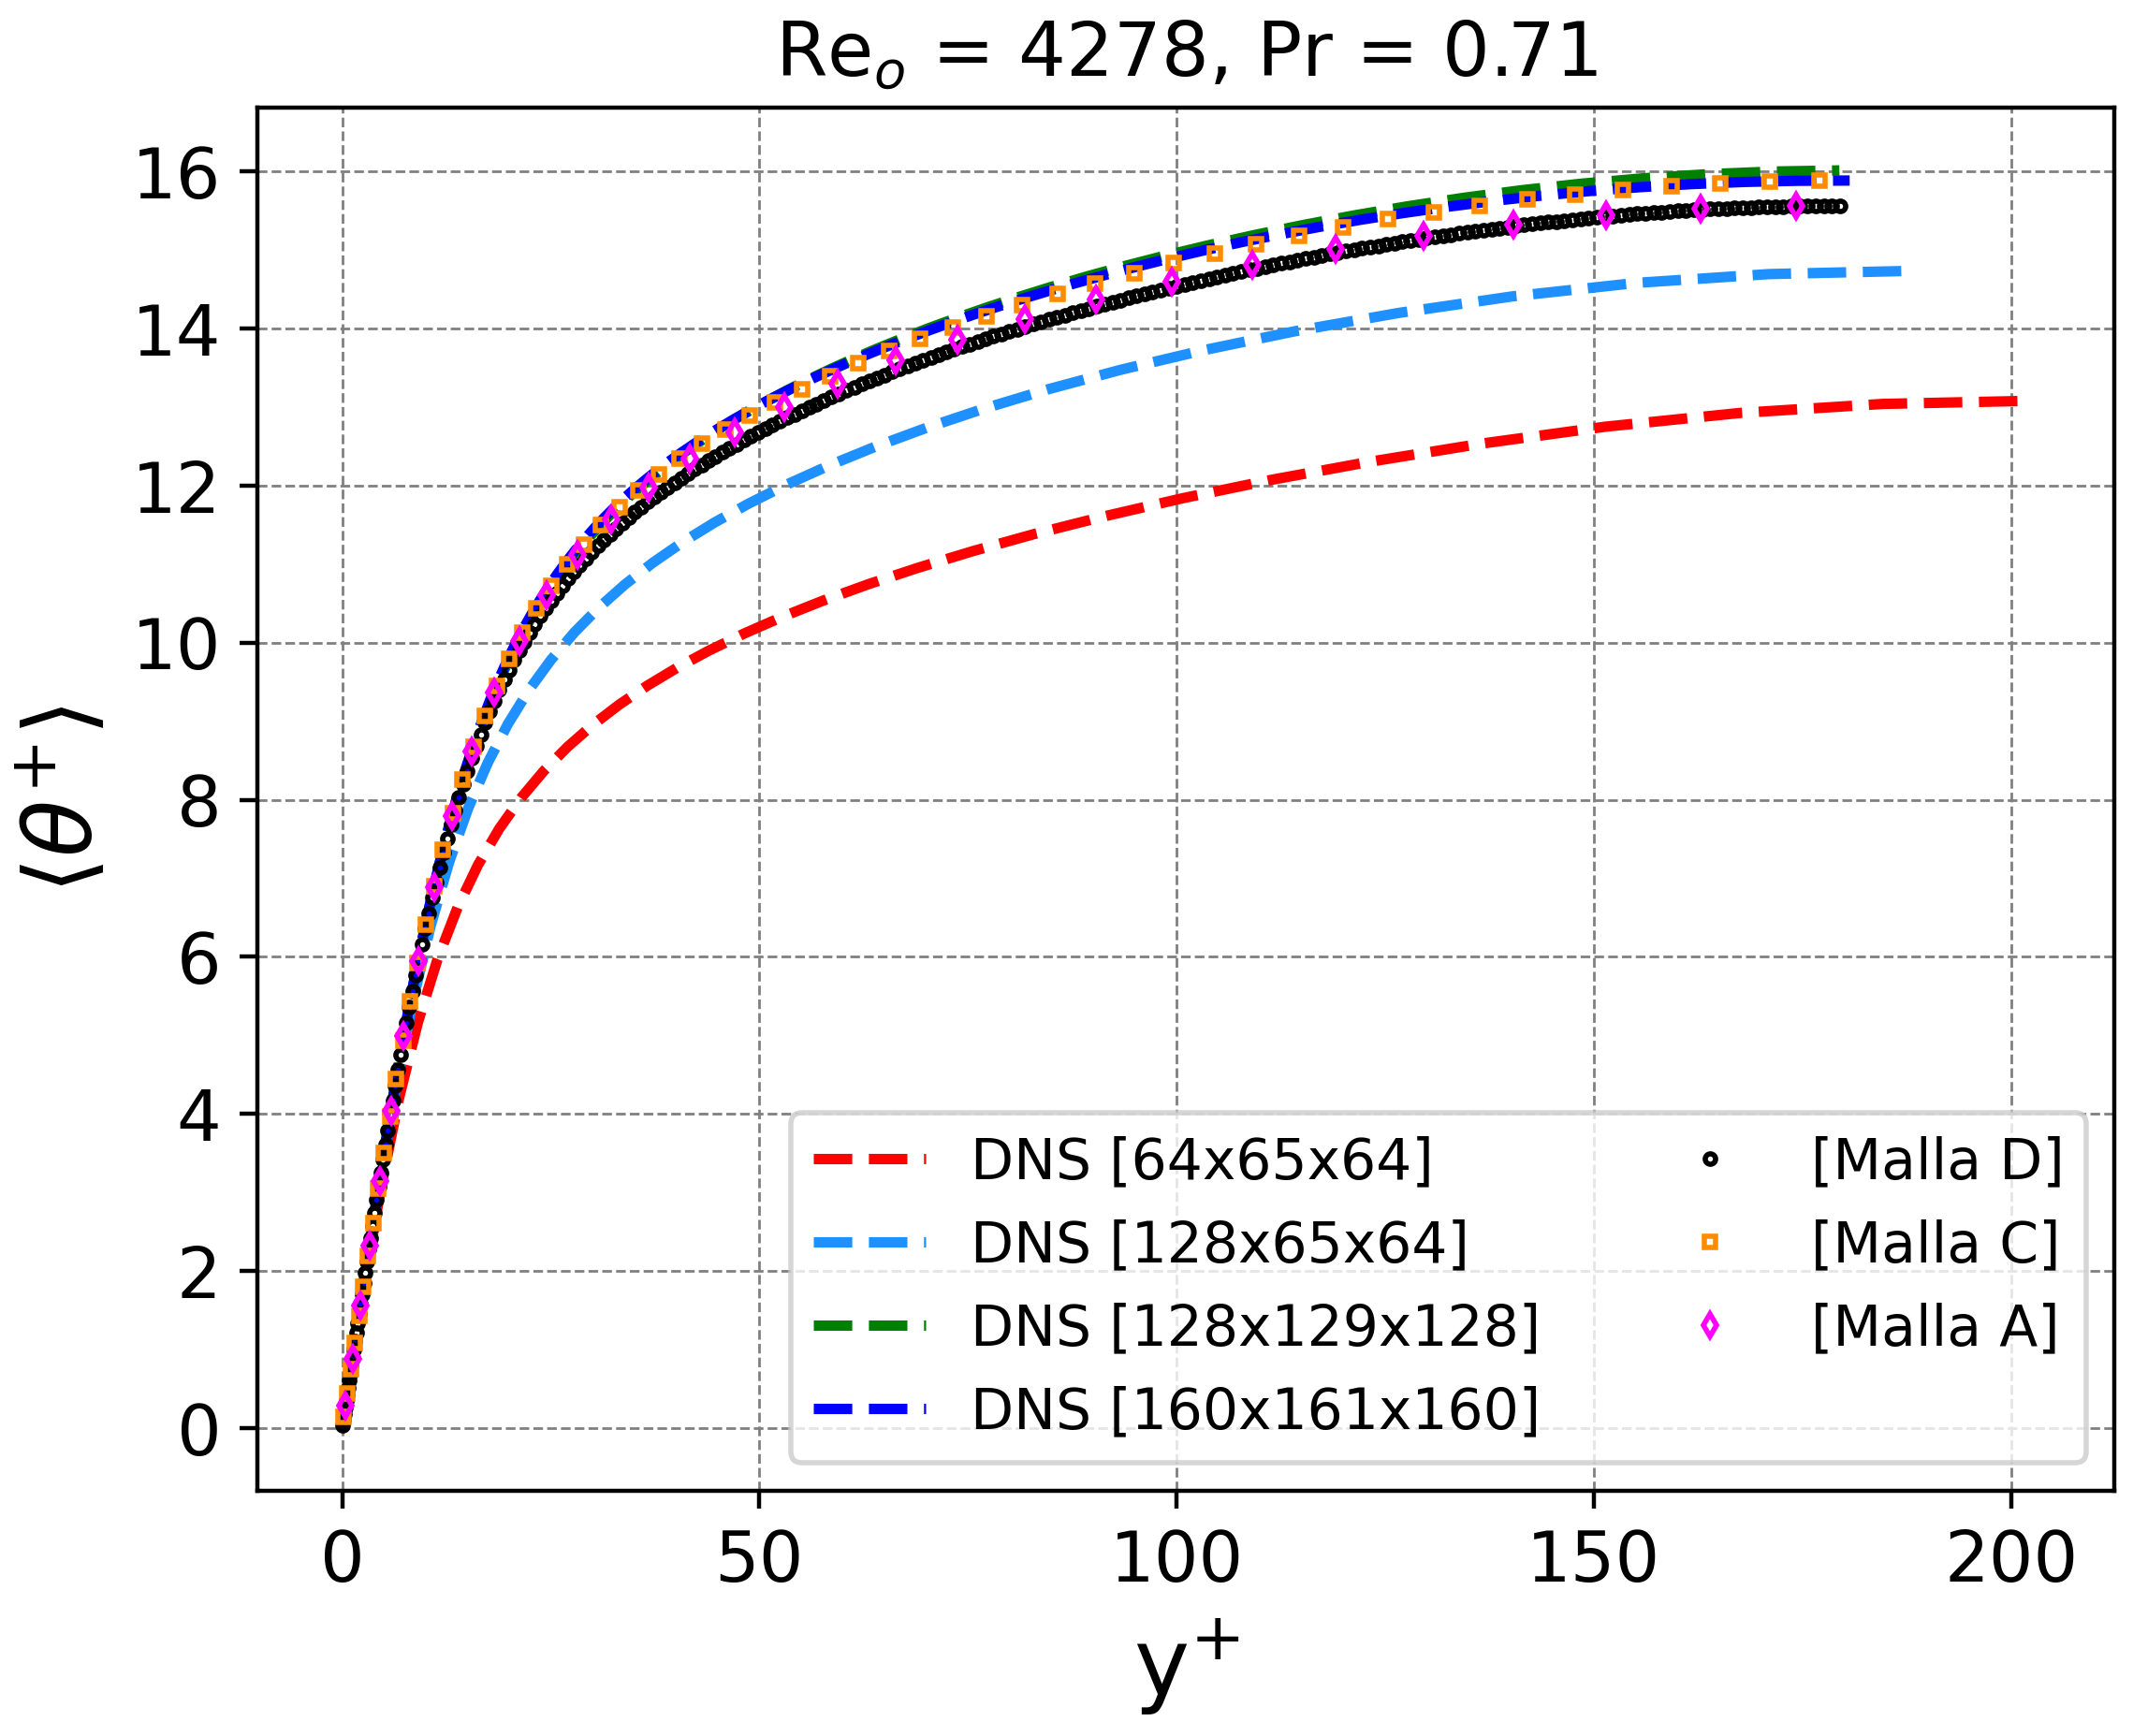
\includegraphics[width=0.49\textwidth]{figures/cap4/kawamura_mesh/tep_theta.png}
    	\label{fig:kmesh-theta}}  
    \subfloat[]{
    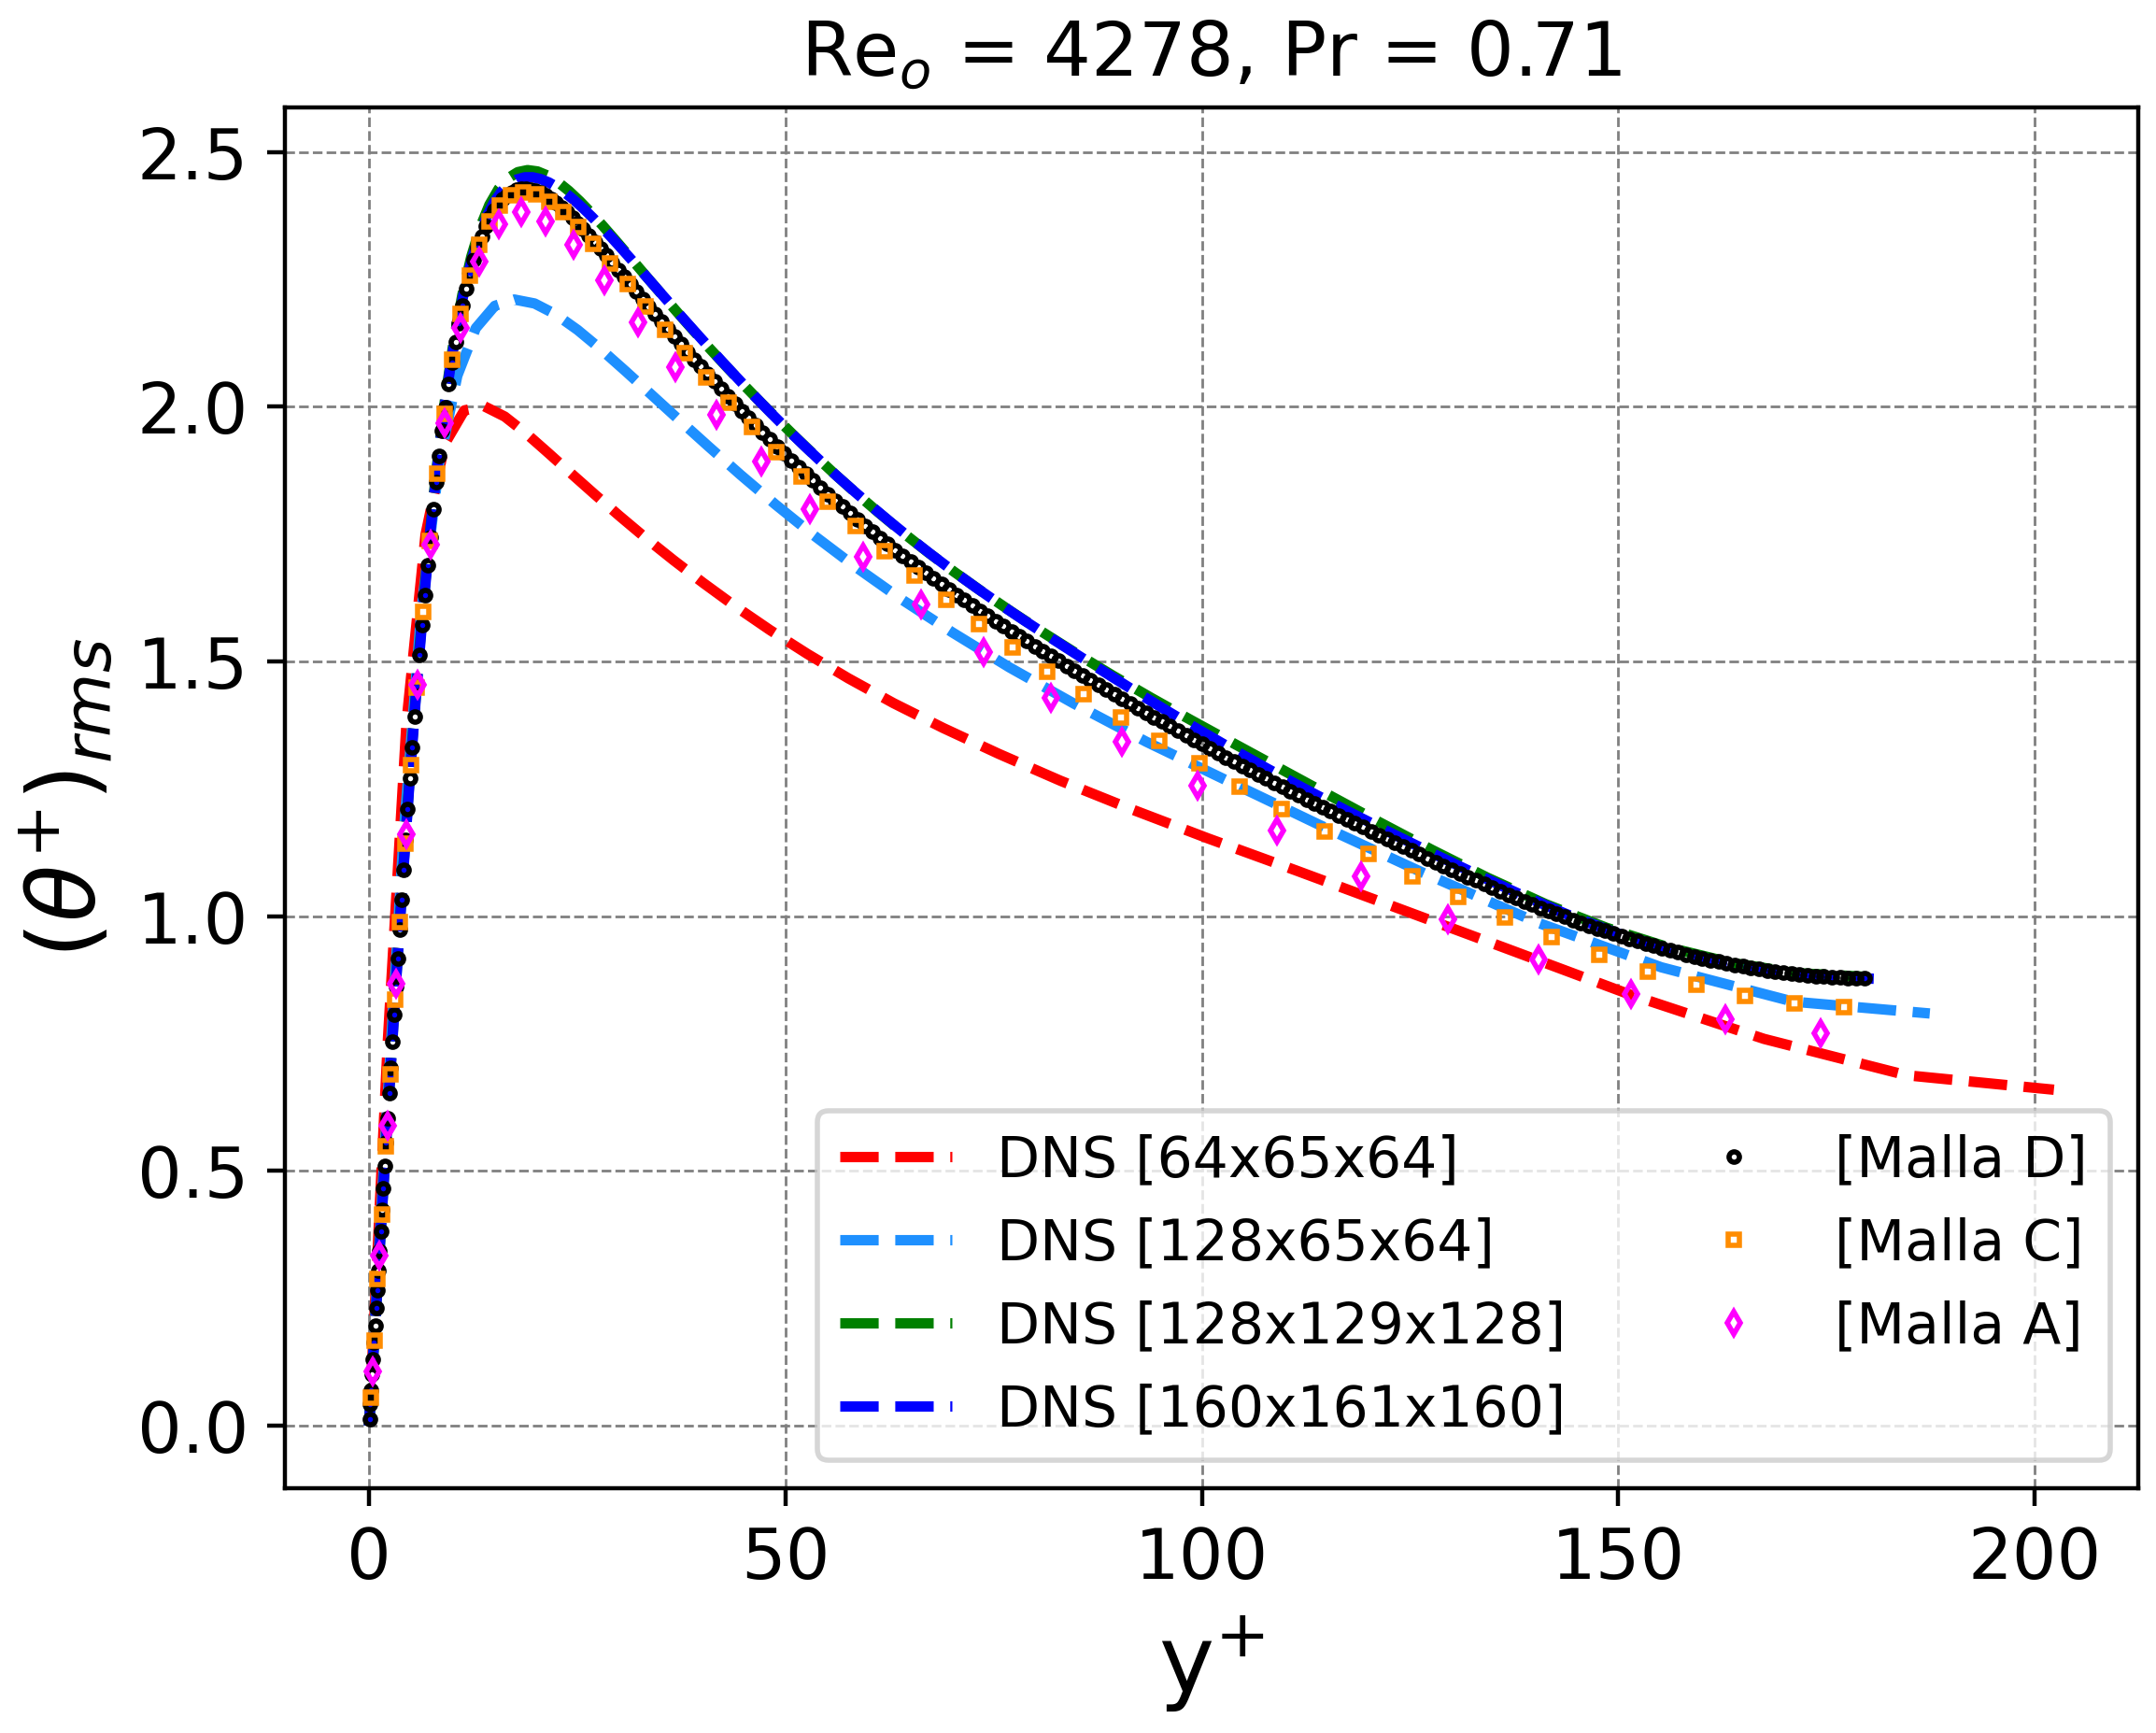
\includegraphics[width=0.49\textwidth]{figures/cap4/kawamura_mesh/tep_thetap_rms.png}
    	\label{fig:kmesh-theta-rms}}  

    \subfloat[]{
    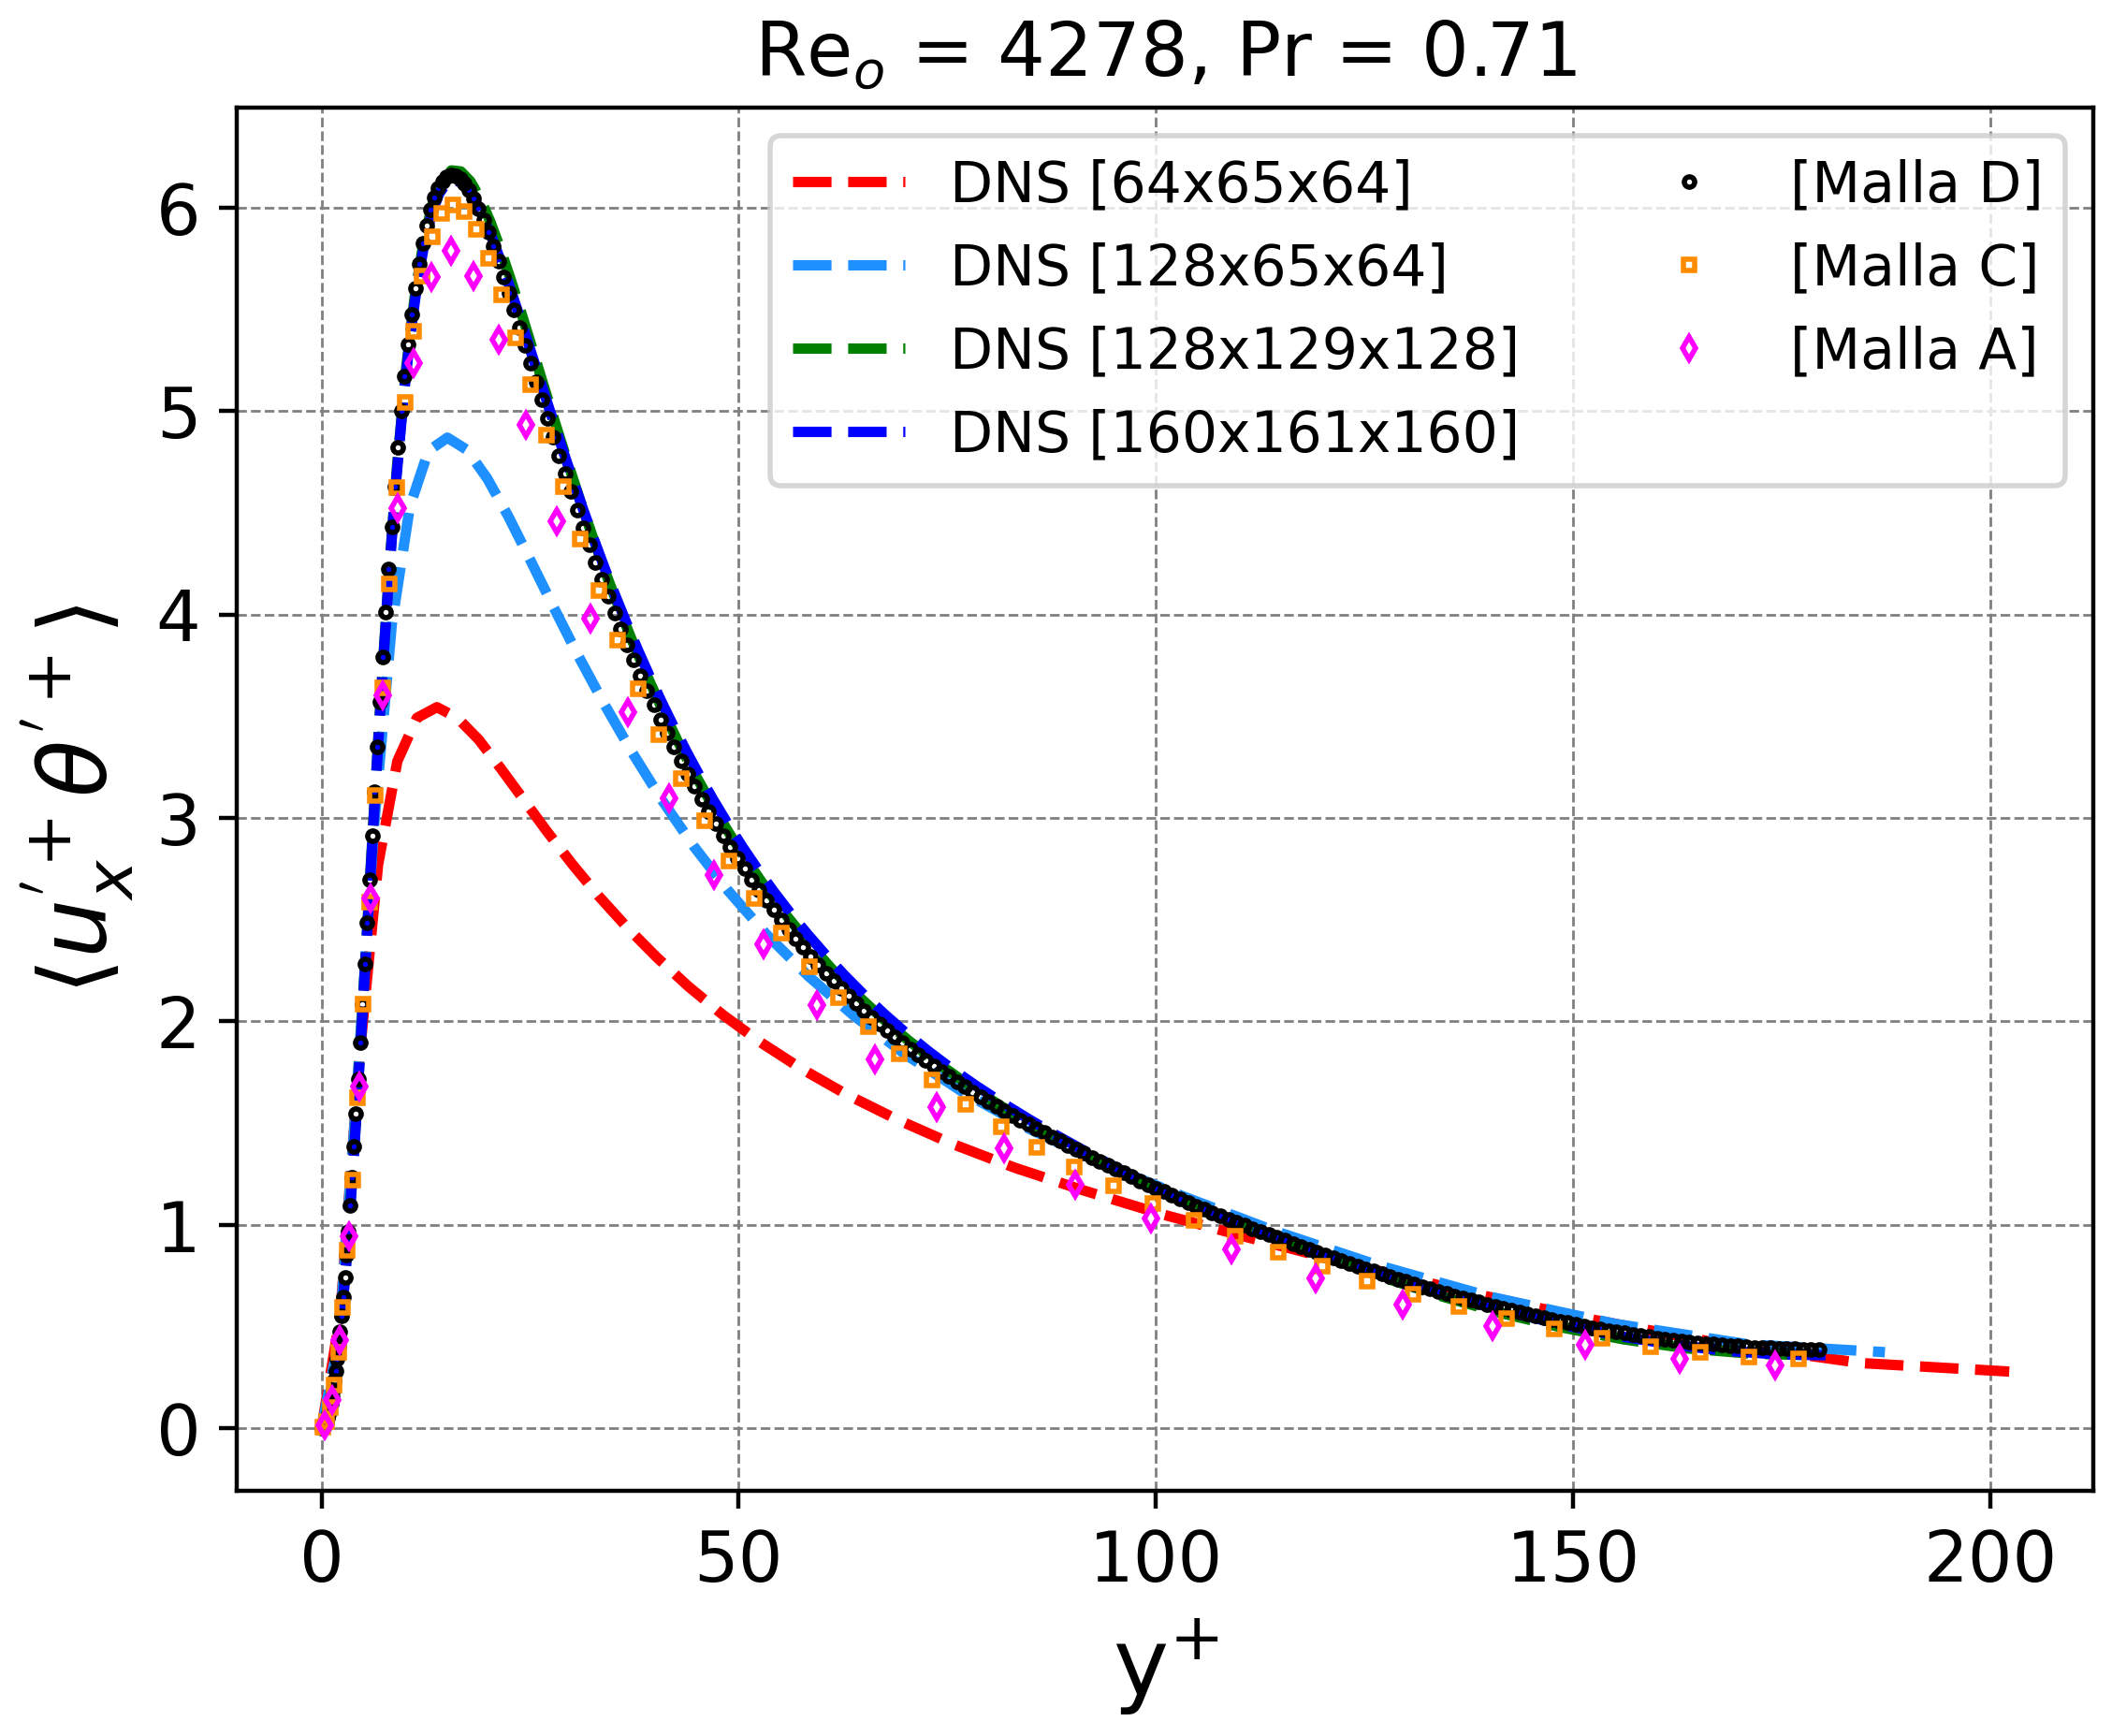
\includegraphics[width=0.49\textwidth]{figures/cap4/kawamura_mesh/tep_up_thetap.png}
    	\label{fig:kmesh-ux-theta}}  
    \subfloat[]{
    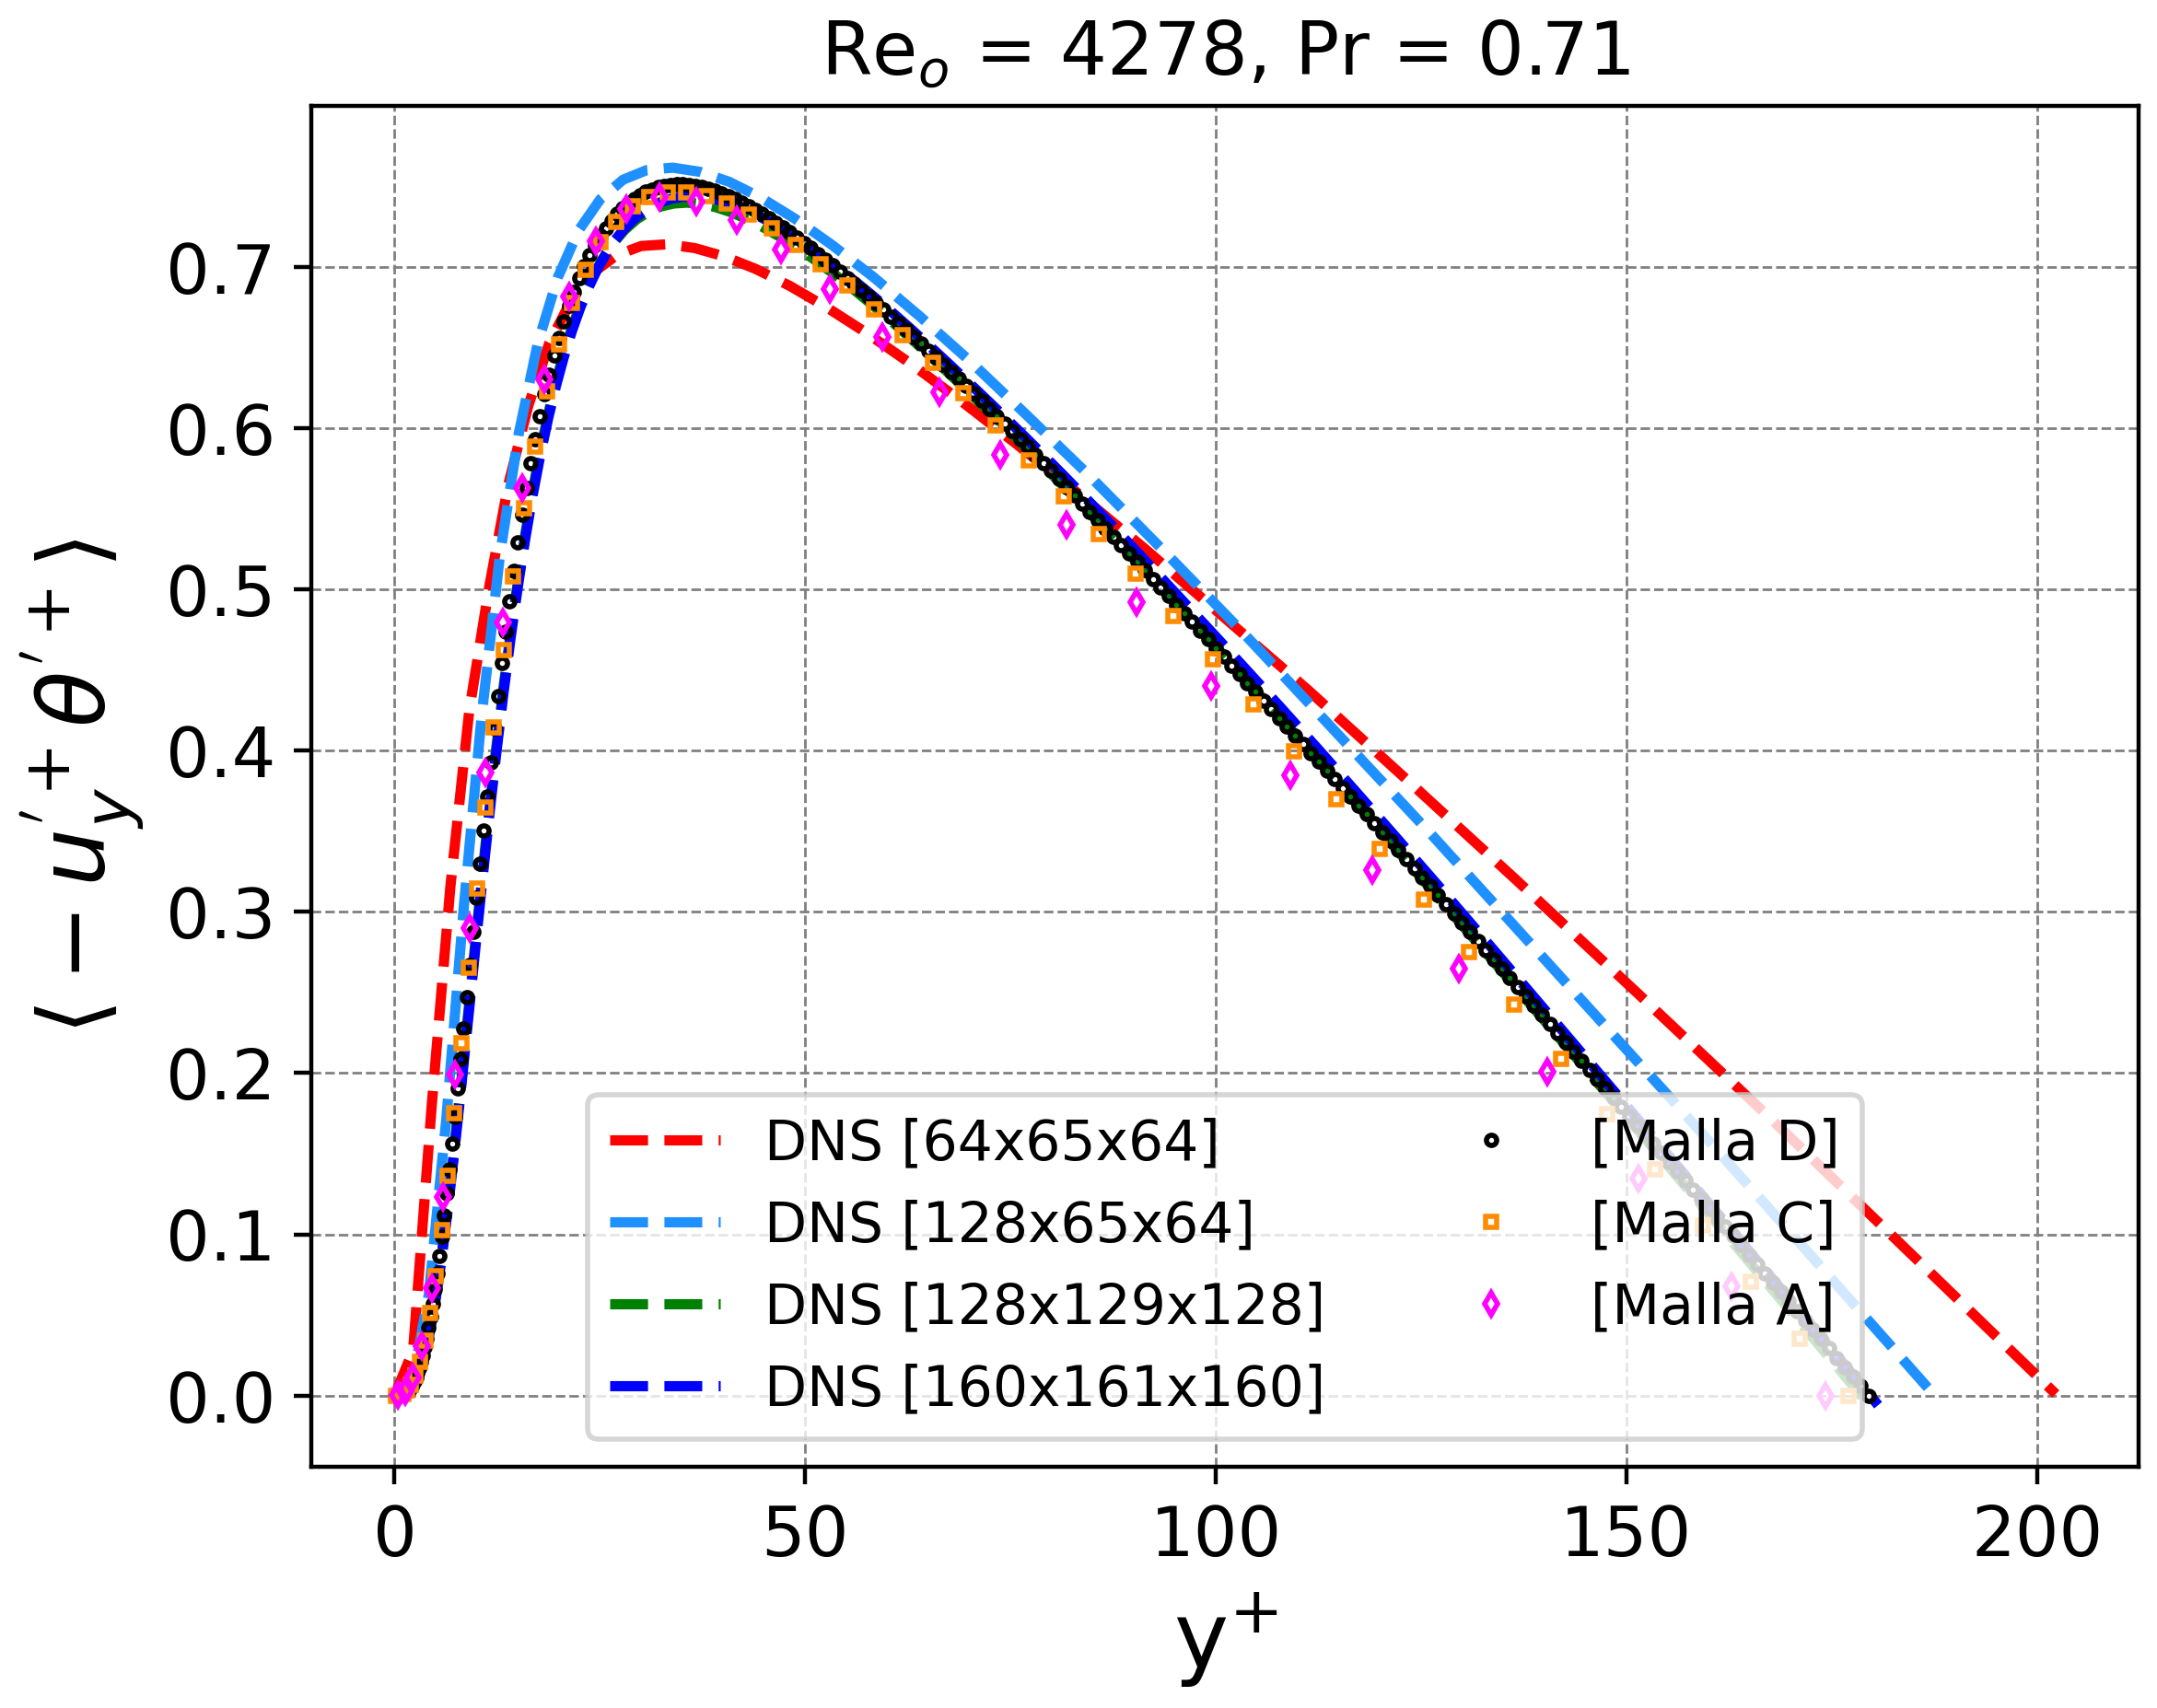
\includegraphics[width=0.49\textwidth]{figures/cap4/kawamura_mesh/tep_vp_thetap.png}
    	\label{fig:kmesh-uy-theta}}  
 \caption{Perfiles de \textbf{(a)} temperatura adimensional media, \textbf{(b)} fluctuaciones RMS de la temperatura adimensional, \textbf{(c)} flujo de calor turbulento en la dirección X, $\langle u^+_x \theta^+ \rangle$, y \textbf{(d)} flujo de calor turbulento en la dirección Y, $\langle u^+_y \theta^+ \rangle$.} 
 \label{fig:kmesh_1}
\end{figure}

\paragraph{Variación del número de Prandtl.}
La segunda parte consiste en emplear la malla M2 para distintos números de Prandtl, en particular, aquellos empleados en el trabajo de Kawamura \textit{et al.}: Pr= 0.025, 0.71, 1 y 7. De igual forma que para la convergencia en malla, en las Figuras \ref{fig:kpr-theta} - \ref{fig:kpr-uy-theta} se muestran los perfiles de las magnitudes $\langle \theta^+ \rangle$, $(\theta^+)_{rms}$, $\langle u^{+ \prime}_x \theta^{+ \prime} \rangle$ y $\langle - u^{+ \prime}_y \theta^{+ \prime} \rangle$, respectivamente. Debe aclararse, además, que el tiempo necesario para alcanzar el régimen estadísticamente estacionario crece con el número de Prandtl.

Nuevamente, se observa que la malla M2 resulta en un compromiso adecuado entre precisión y costo computacional para replicar con suficiente fidelidad\footnote{Por ejemplo, para $\text{Pr}=7$, se observa gráficamente que el perfil $(\theta^+)_{\text{rms}}$ presenta en $y^+ \simeq 62\text{.}5$ una discrepancia entre la simulación propia y la de referencia; sin embargo, su error relativo es inferior al 5 \%.} las simulaciones de \linebreak Kawamura \textit{et al}. 

\begin{figure}[H]
 \centering
  \subfloat[]{
    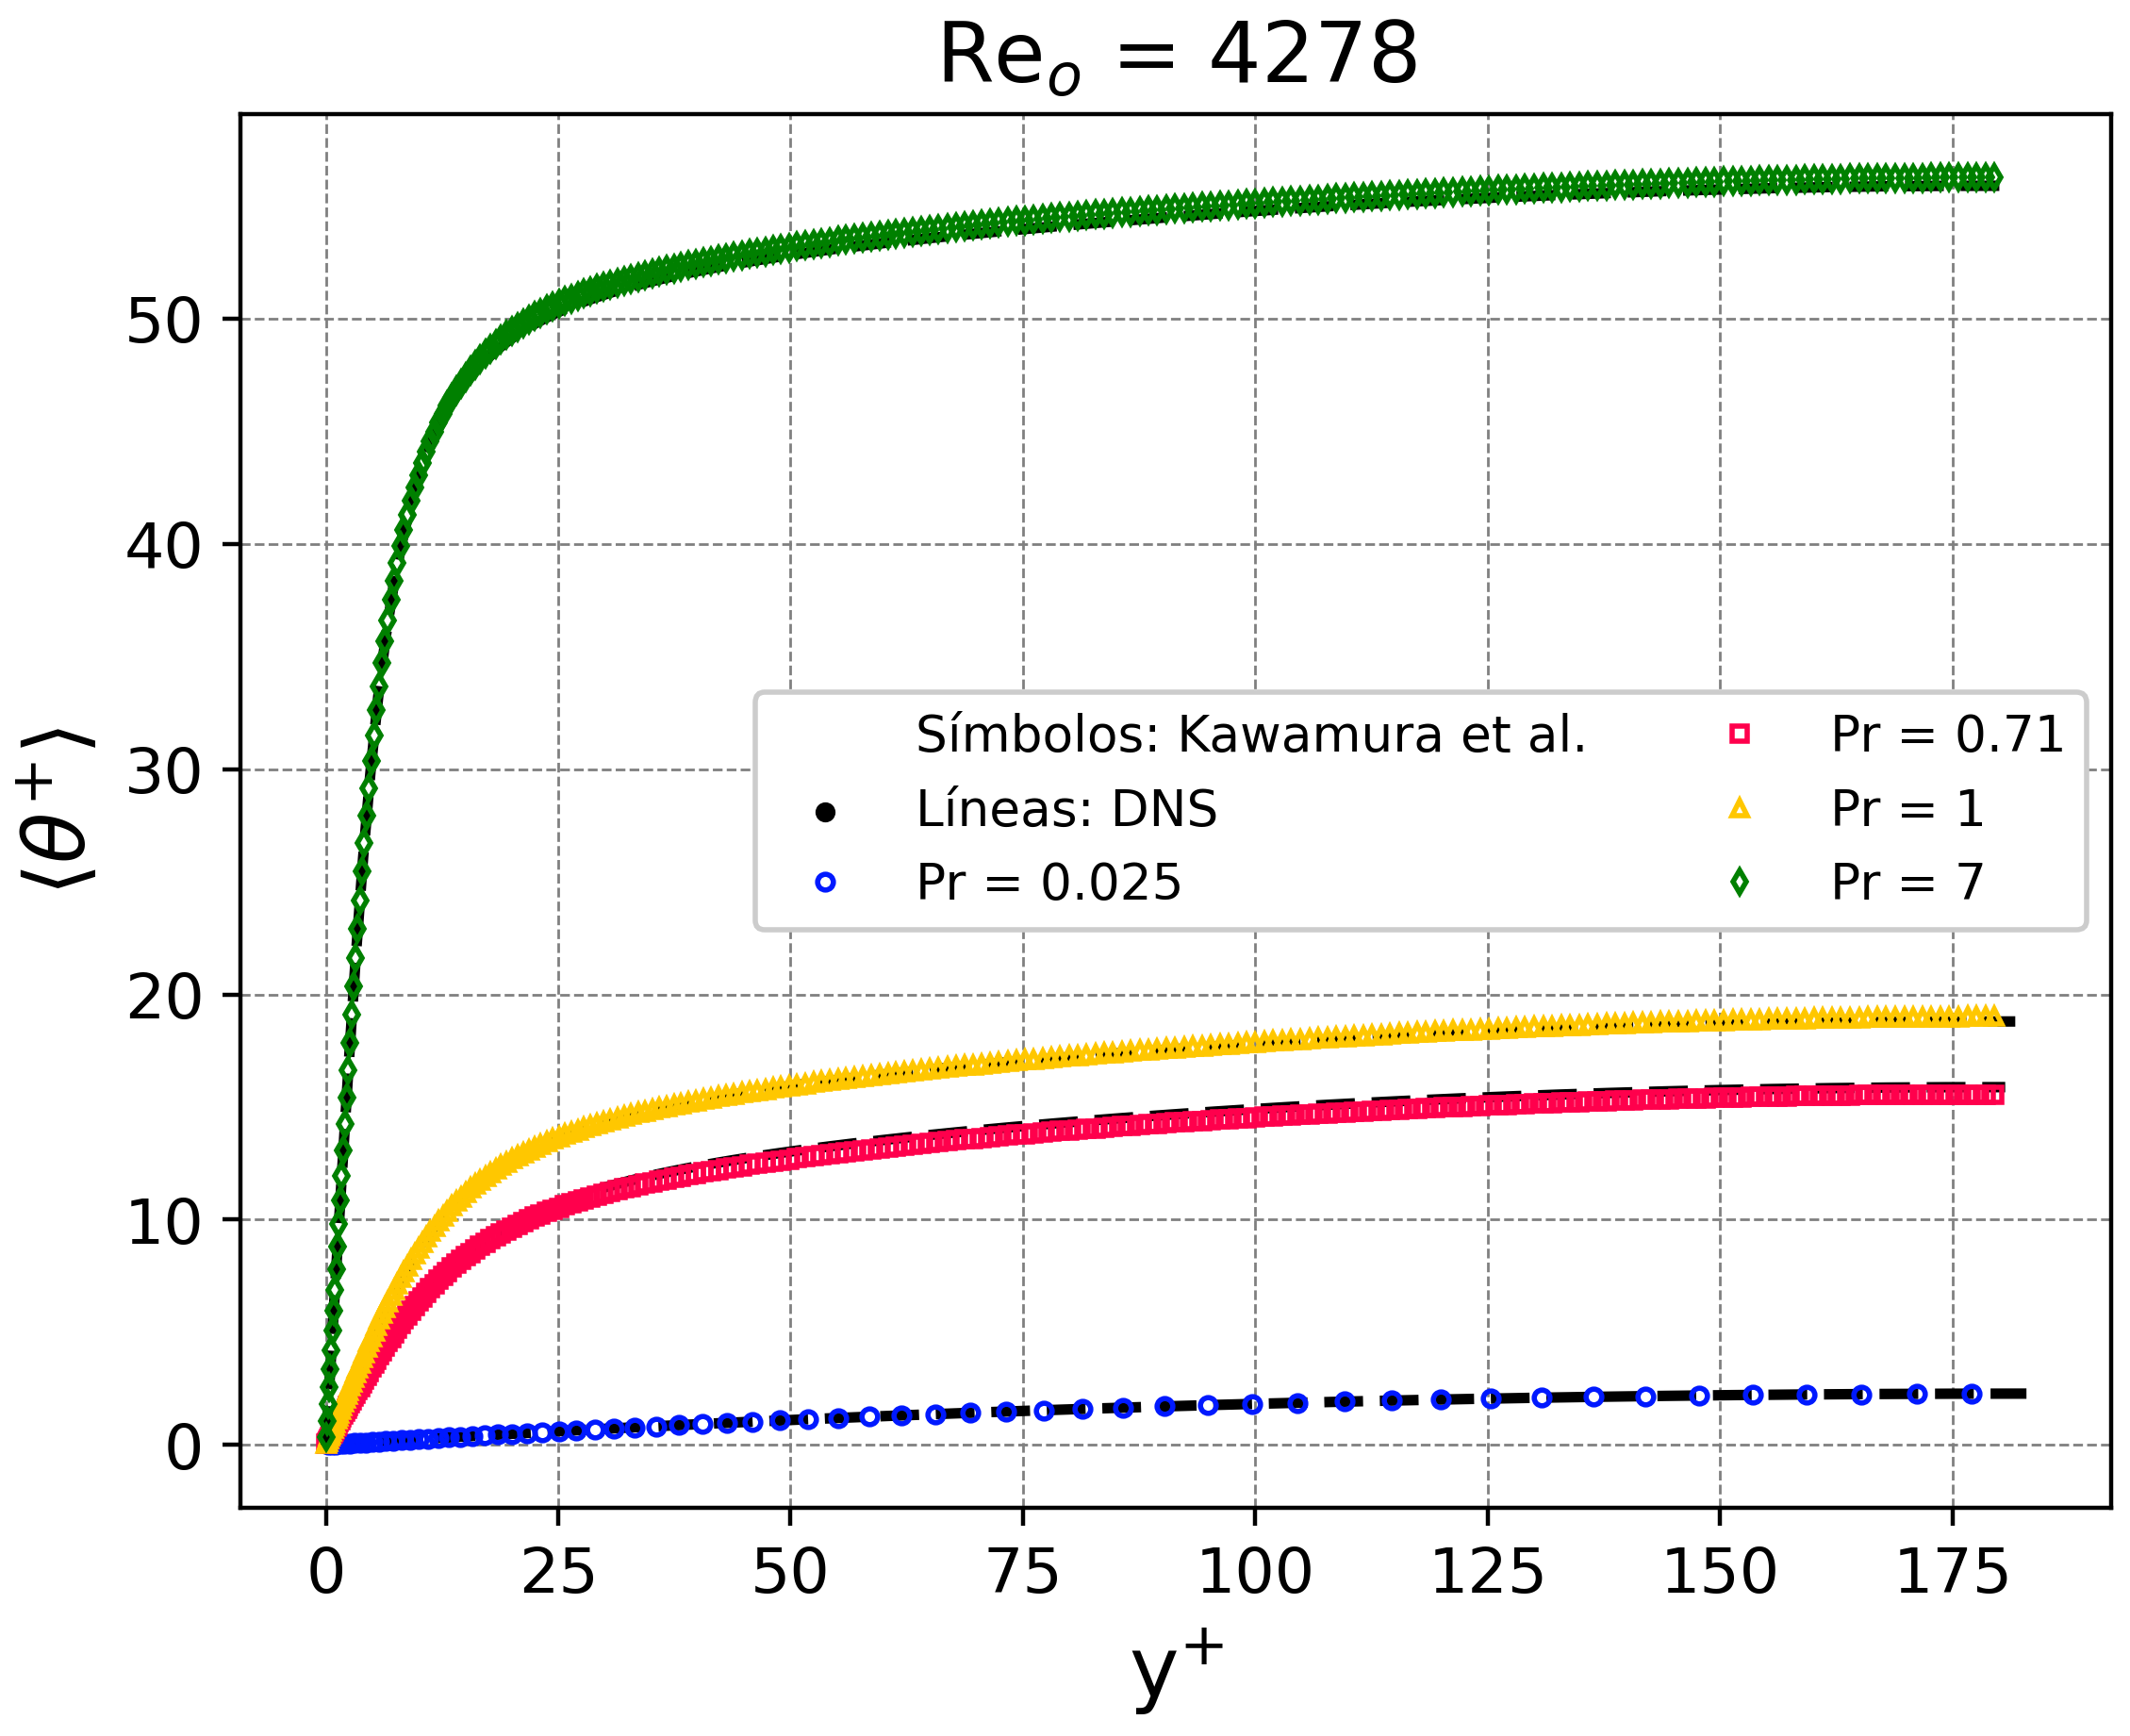
\includegraphics[width=0.49\textwidth]{figures/cap4/kawamura_prs/tep_theta.png}
    \label{fig:kpr-theta}}  
    \subfloat[]{
    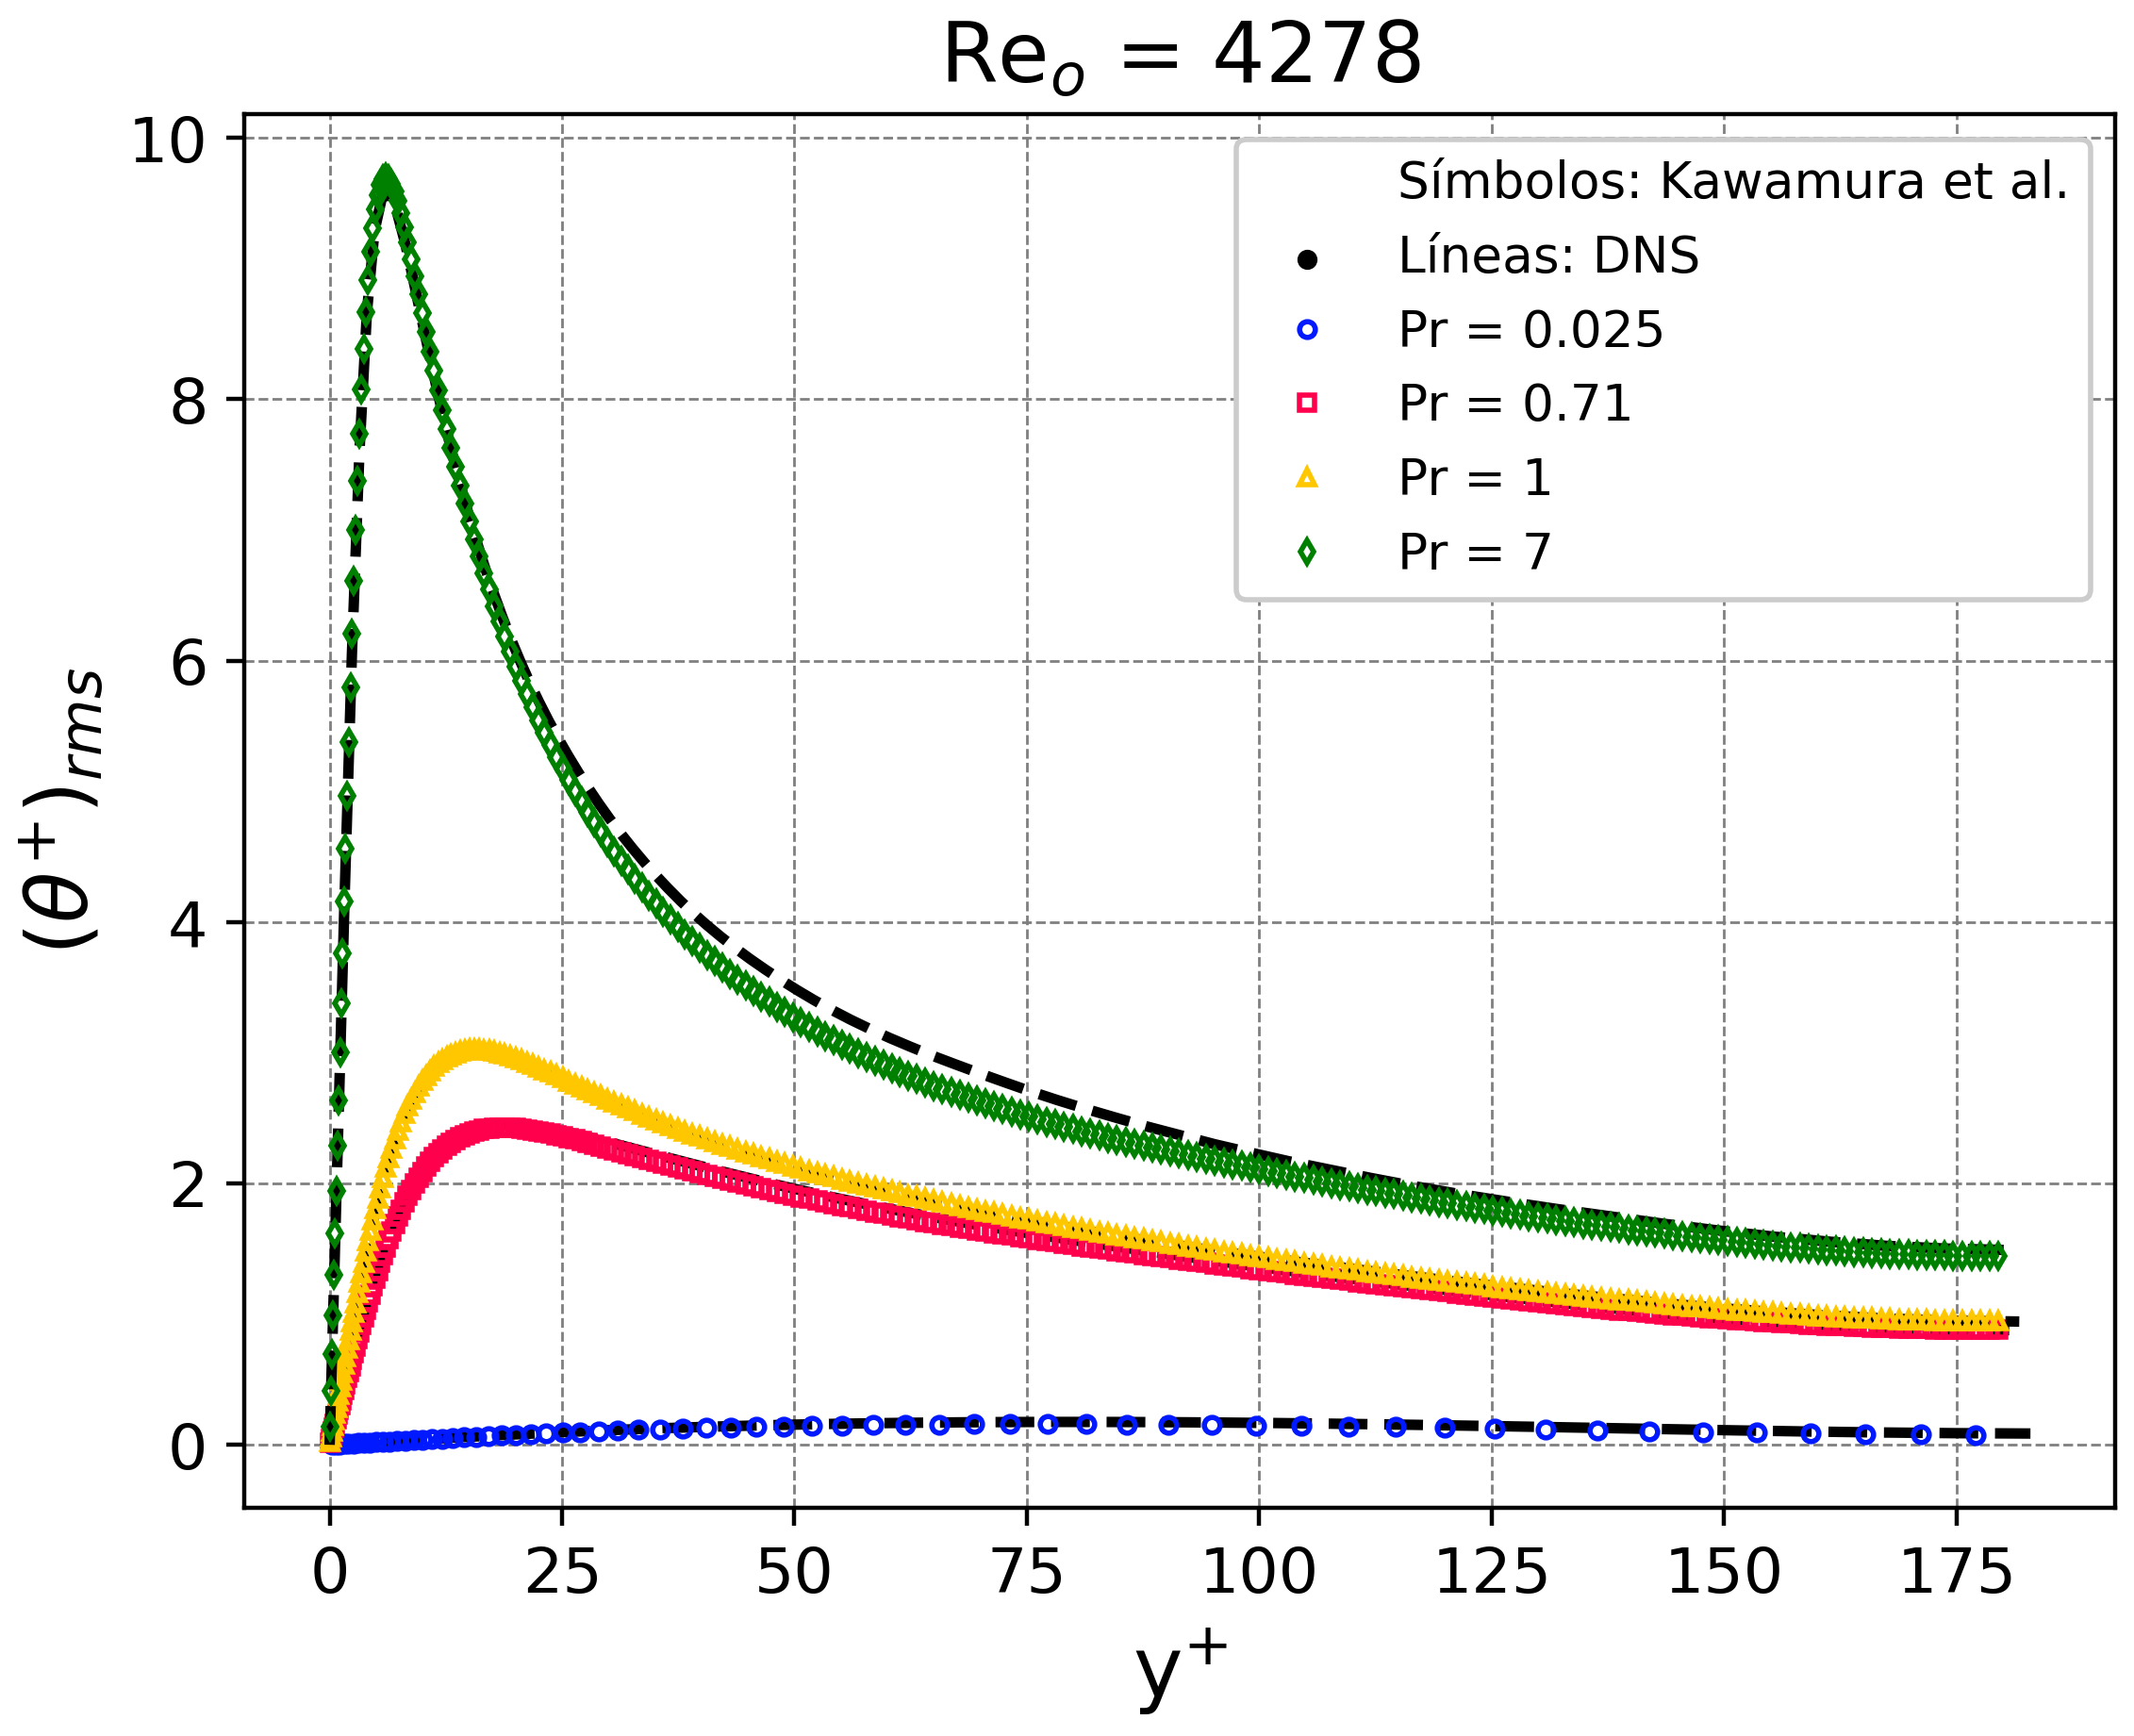
\includegraphics[width=0.49\textwidth]{figures/cap4/kawamura_prs/tep_thetap_rms.png}
    \label{fig:kpr-theta-rms}}  
 
  \subfloat[]{
    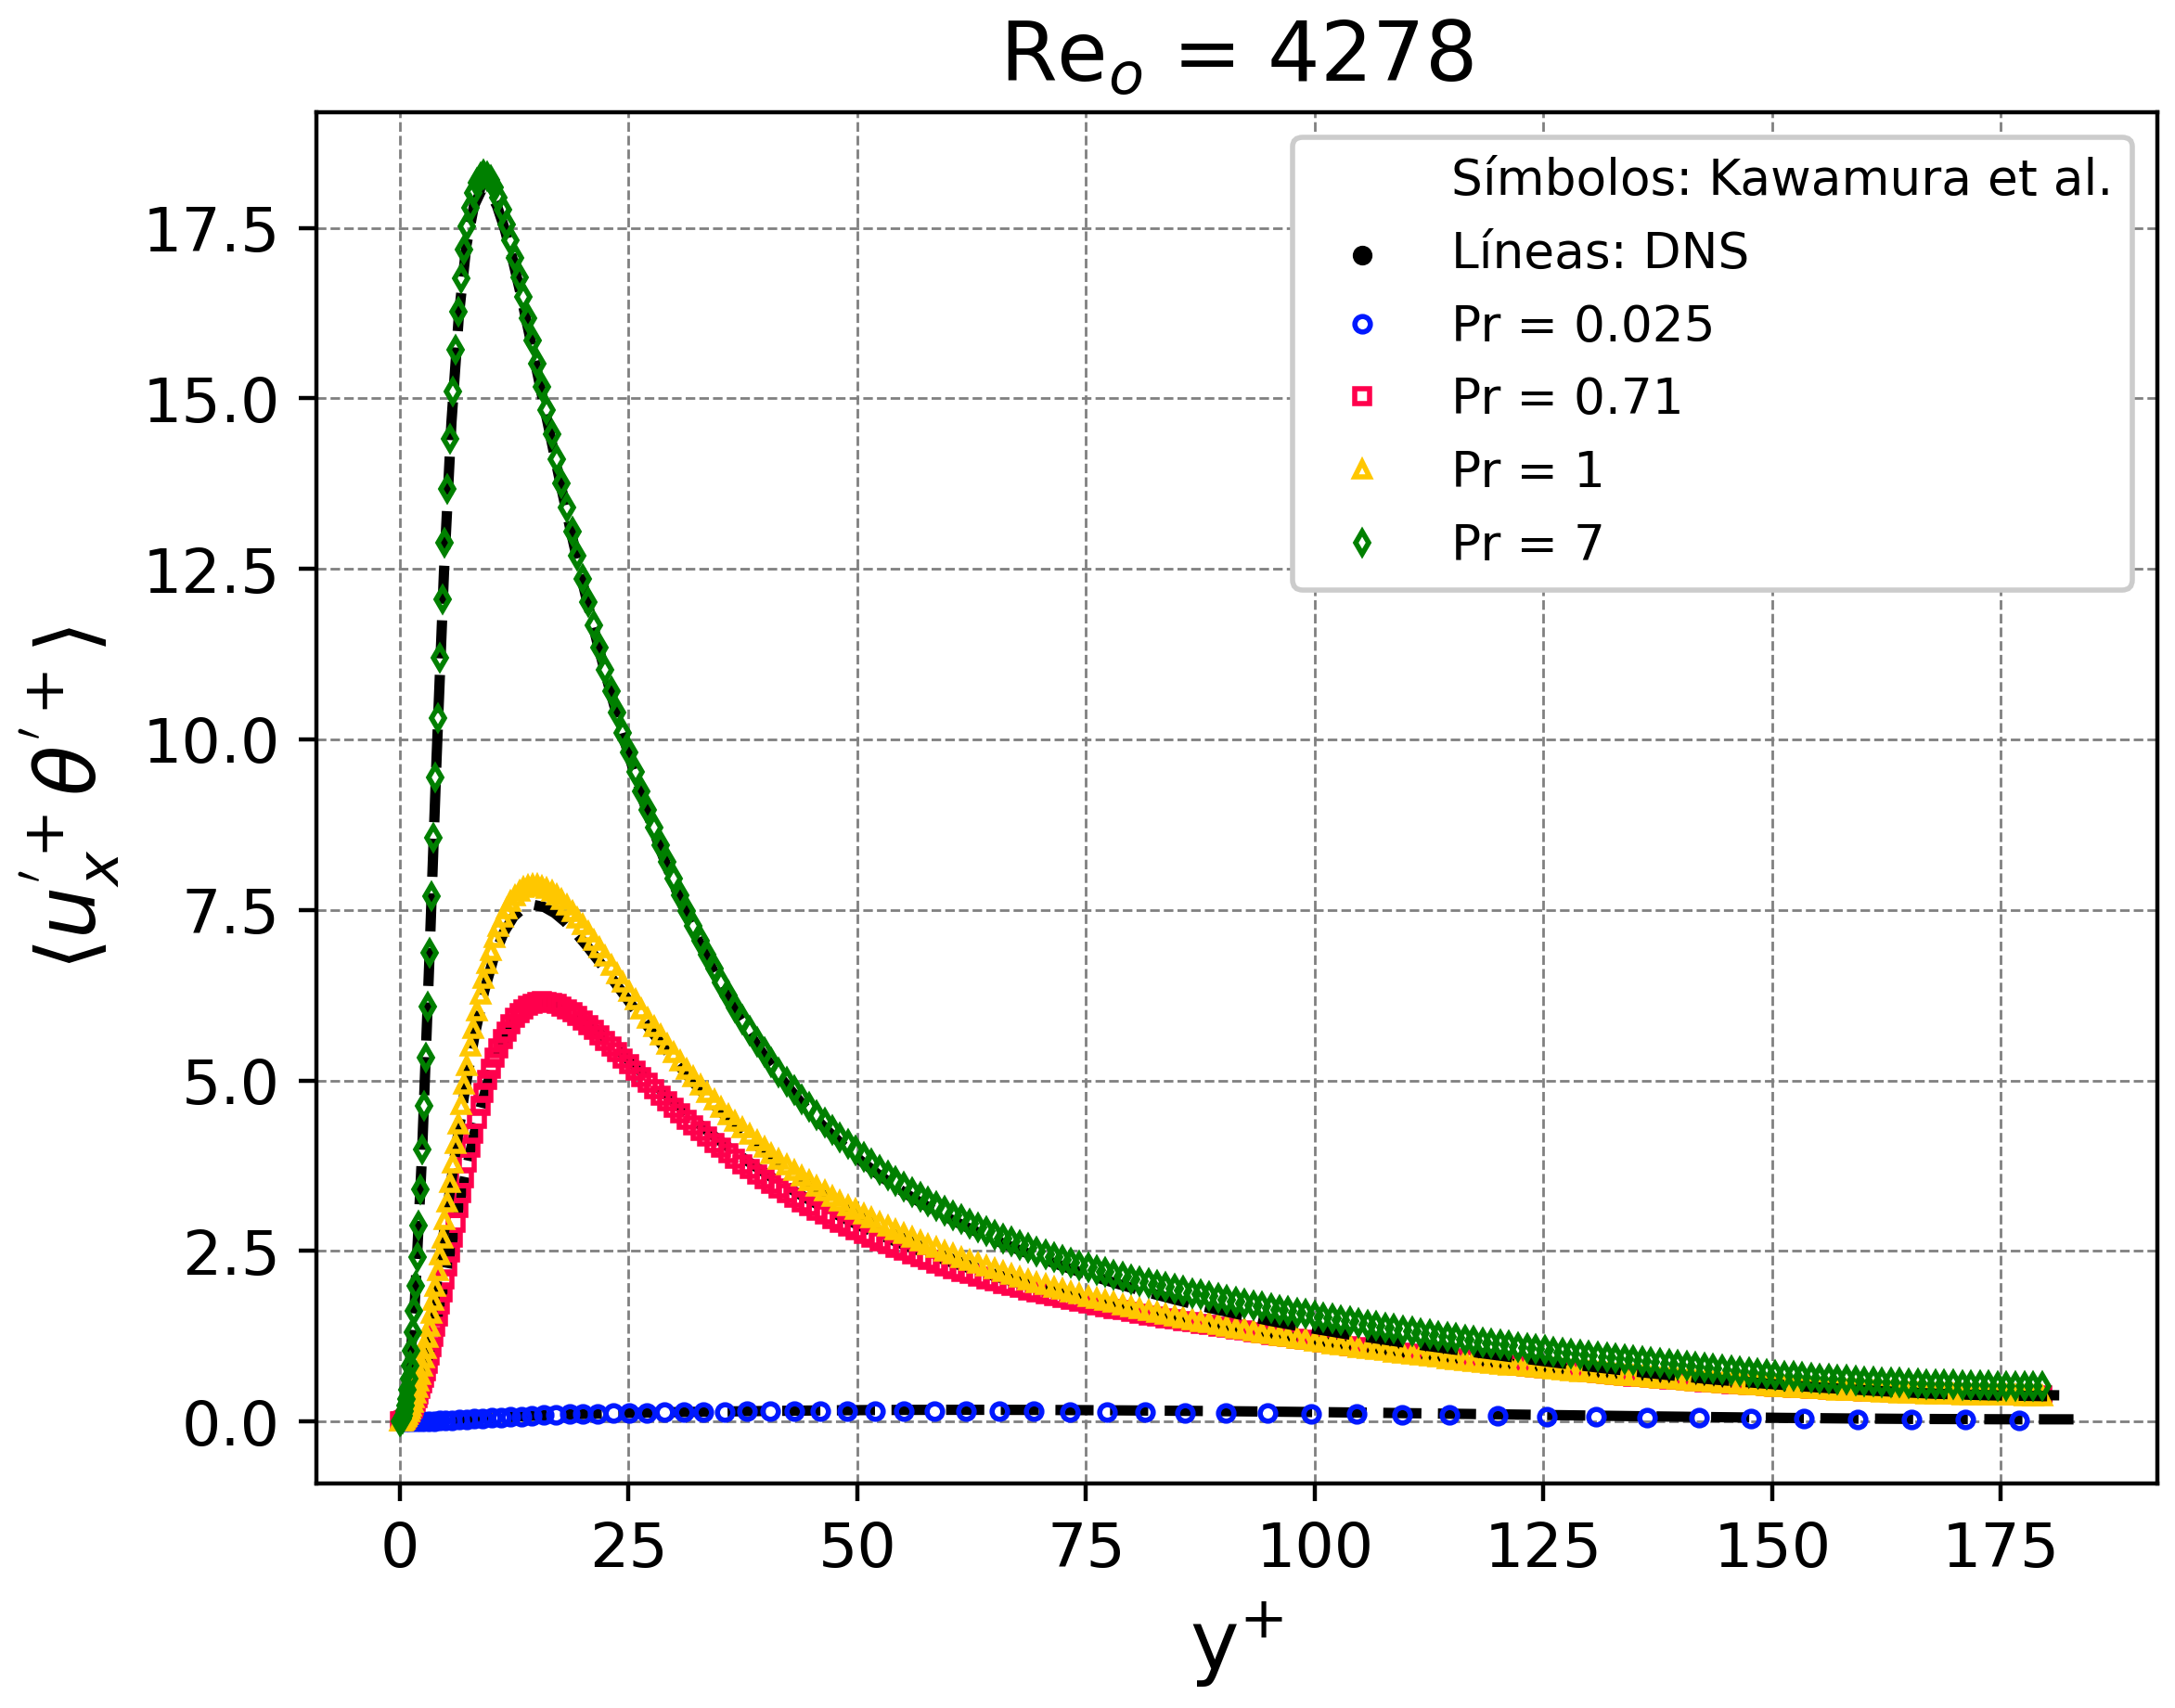
\includegraphics[width=0.49\textwidth]{figures/cap4/kawamura_prs/tep_up_thetap.png}
    \label{fig:kpr-ux-theta}}  
    \subfloat[]{
    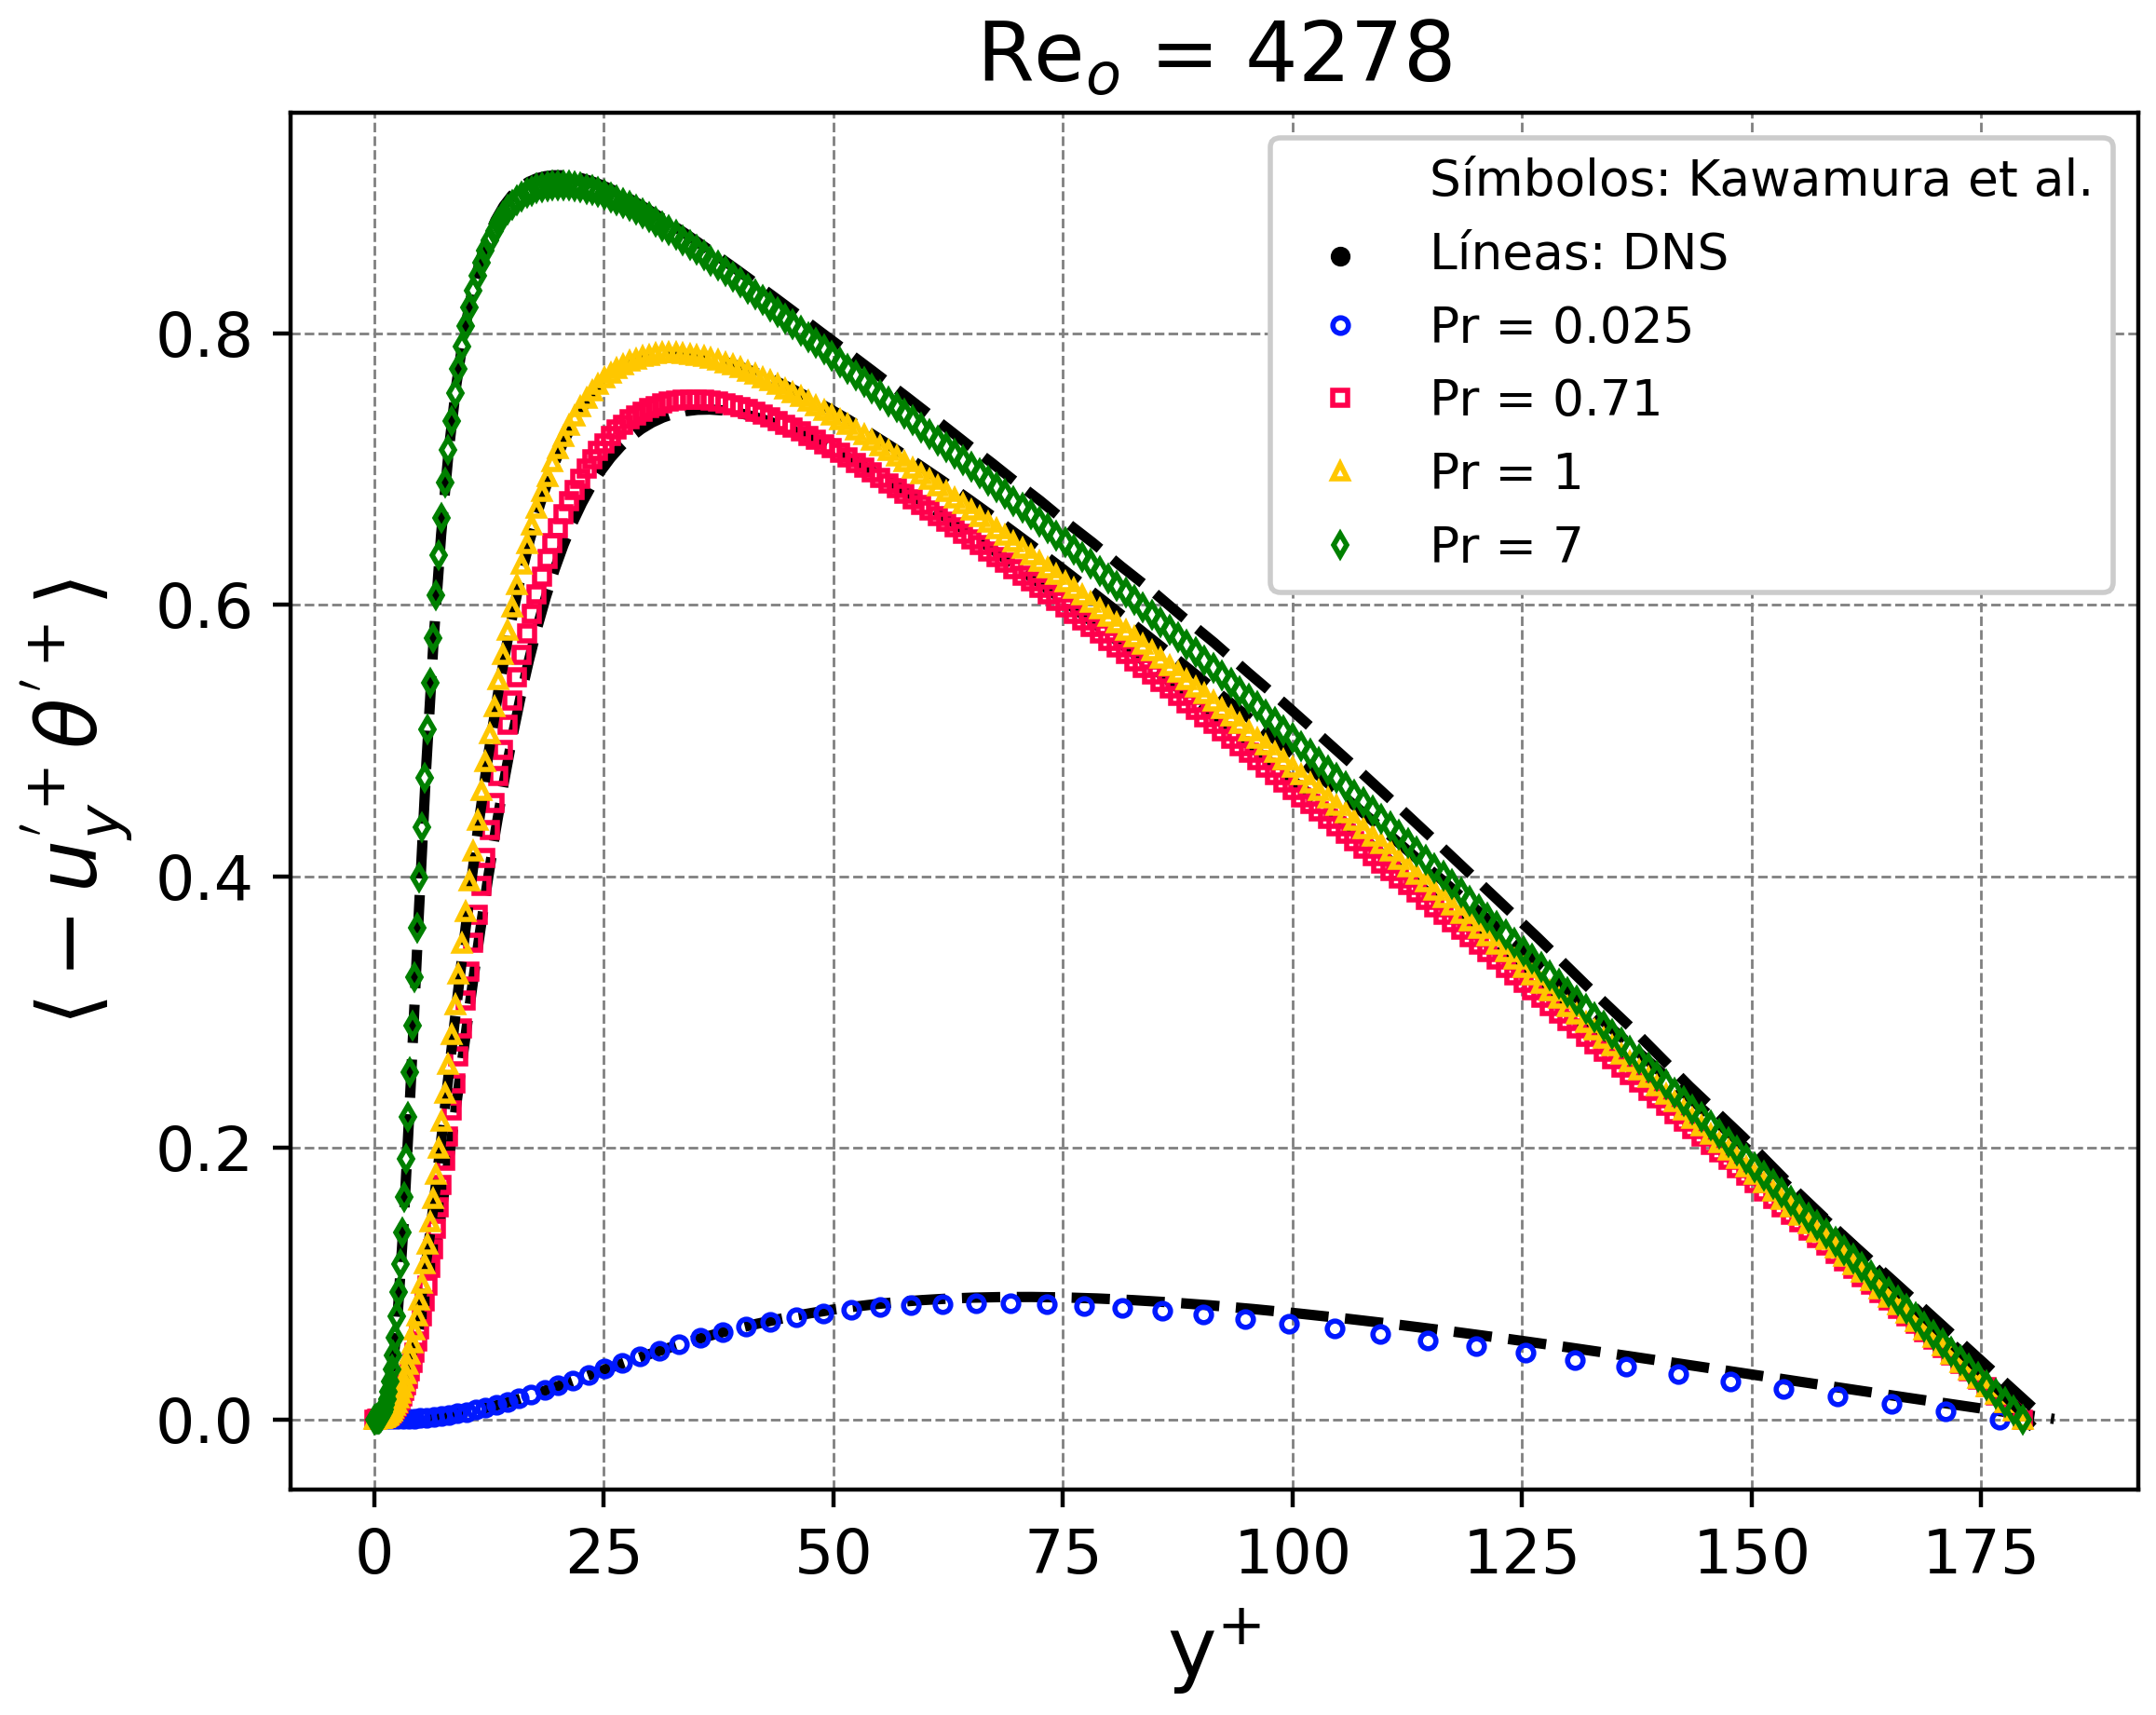
\includegraphics[width=0.49\textwidth]{figures/cap4/kawamura_prs/tep_vp_thetap.png}
    \label{fig:kpr-uy-theta}}  
 \caption{Para diferentes números de Pr se tienen los perfiles de \textbf{(a)} temperatura adimensional media, \textbf{(b)} fluctuaciones RMS de la temperatura adimensional, \textbf{(c)} flujo de calor turbulento en la dirección X, $\langle u^+_x \theta^+ \rangle$, y \textbf{(d)} flujo de calor turbulento en la dirección Y, $\langle u^+_y \theta^+ \rangle$.} 
 \label{fig:kpr_1}
\end{figure}


\subsection{Situación III. Canal turbulento en régimen laminar con convección mixta y $q''_w$ constante} \label{sec:mix-laminar}

Hasta aquí, la herramienta numérica XC3D se ha validado en aspectos hidrodinámicos y térmicos bajo convección forzada. Como punto de partida hacia el régimen de convección mixta, se realizan simulaciones considerando un régimen laminar con Re$_o$=100, Pr=1 y distintos números de Rayleigh (Ra = -25, -100, 75, 150, 250) a fin de evaluar el desempeño de XC3D frente a la influencia de la fuerza boyante. En todas las simulaciones se utiliza la malla M0. A diferencia de los apartados anteriores, en estas simulaciones no se impone ninguna condición adicional en el flujo con la intención de acelerar el paso al régimen turbulento, ya que estamos tratando con soluciones laminares.

Se comparan los perfiles de velocidad \textit{streamwise} y de temperatura adimensional con las soluciones analíticas de Chen y Chung \cite{chen1996linear}, dadas por las ecuaciones \ref{eq:vel_asist_boyant} - \ref{eq:theta_opo_boyant}. Los mismos se encuentran en la forma adimensional descrita en el Capítulo \ref{cap:modelo}. En las Figuras \ref{fig:chen-ux} y \ref{fig:chen-theta}, las soluciones analíticas se muestran con anillos negros; asimismo, se incluye el caso con $\text{Ra}=0$ ($\Pi=0$) como referencia (línea azul a trazos). Se aprecia una excelente concordancia entre las soluciones analíticas y las simulaciones DNS, tanto para flujo descendente ($\text{Ra}<0$) como para flujo ascendente ($\text{Ra}>0$). En consecuencia, la malla M0 (la opción computacionalmente más económica) reproduce con alta fidelidad las soluciones laminares de Chen y Chung. 

\begin{figure}[H]
 \centering
  \subfloat[]{
    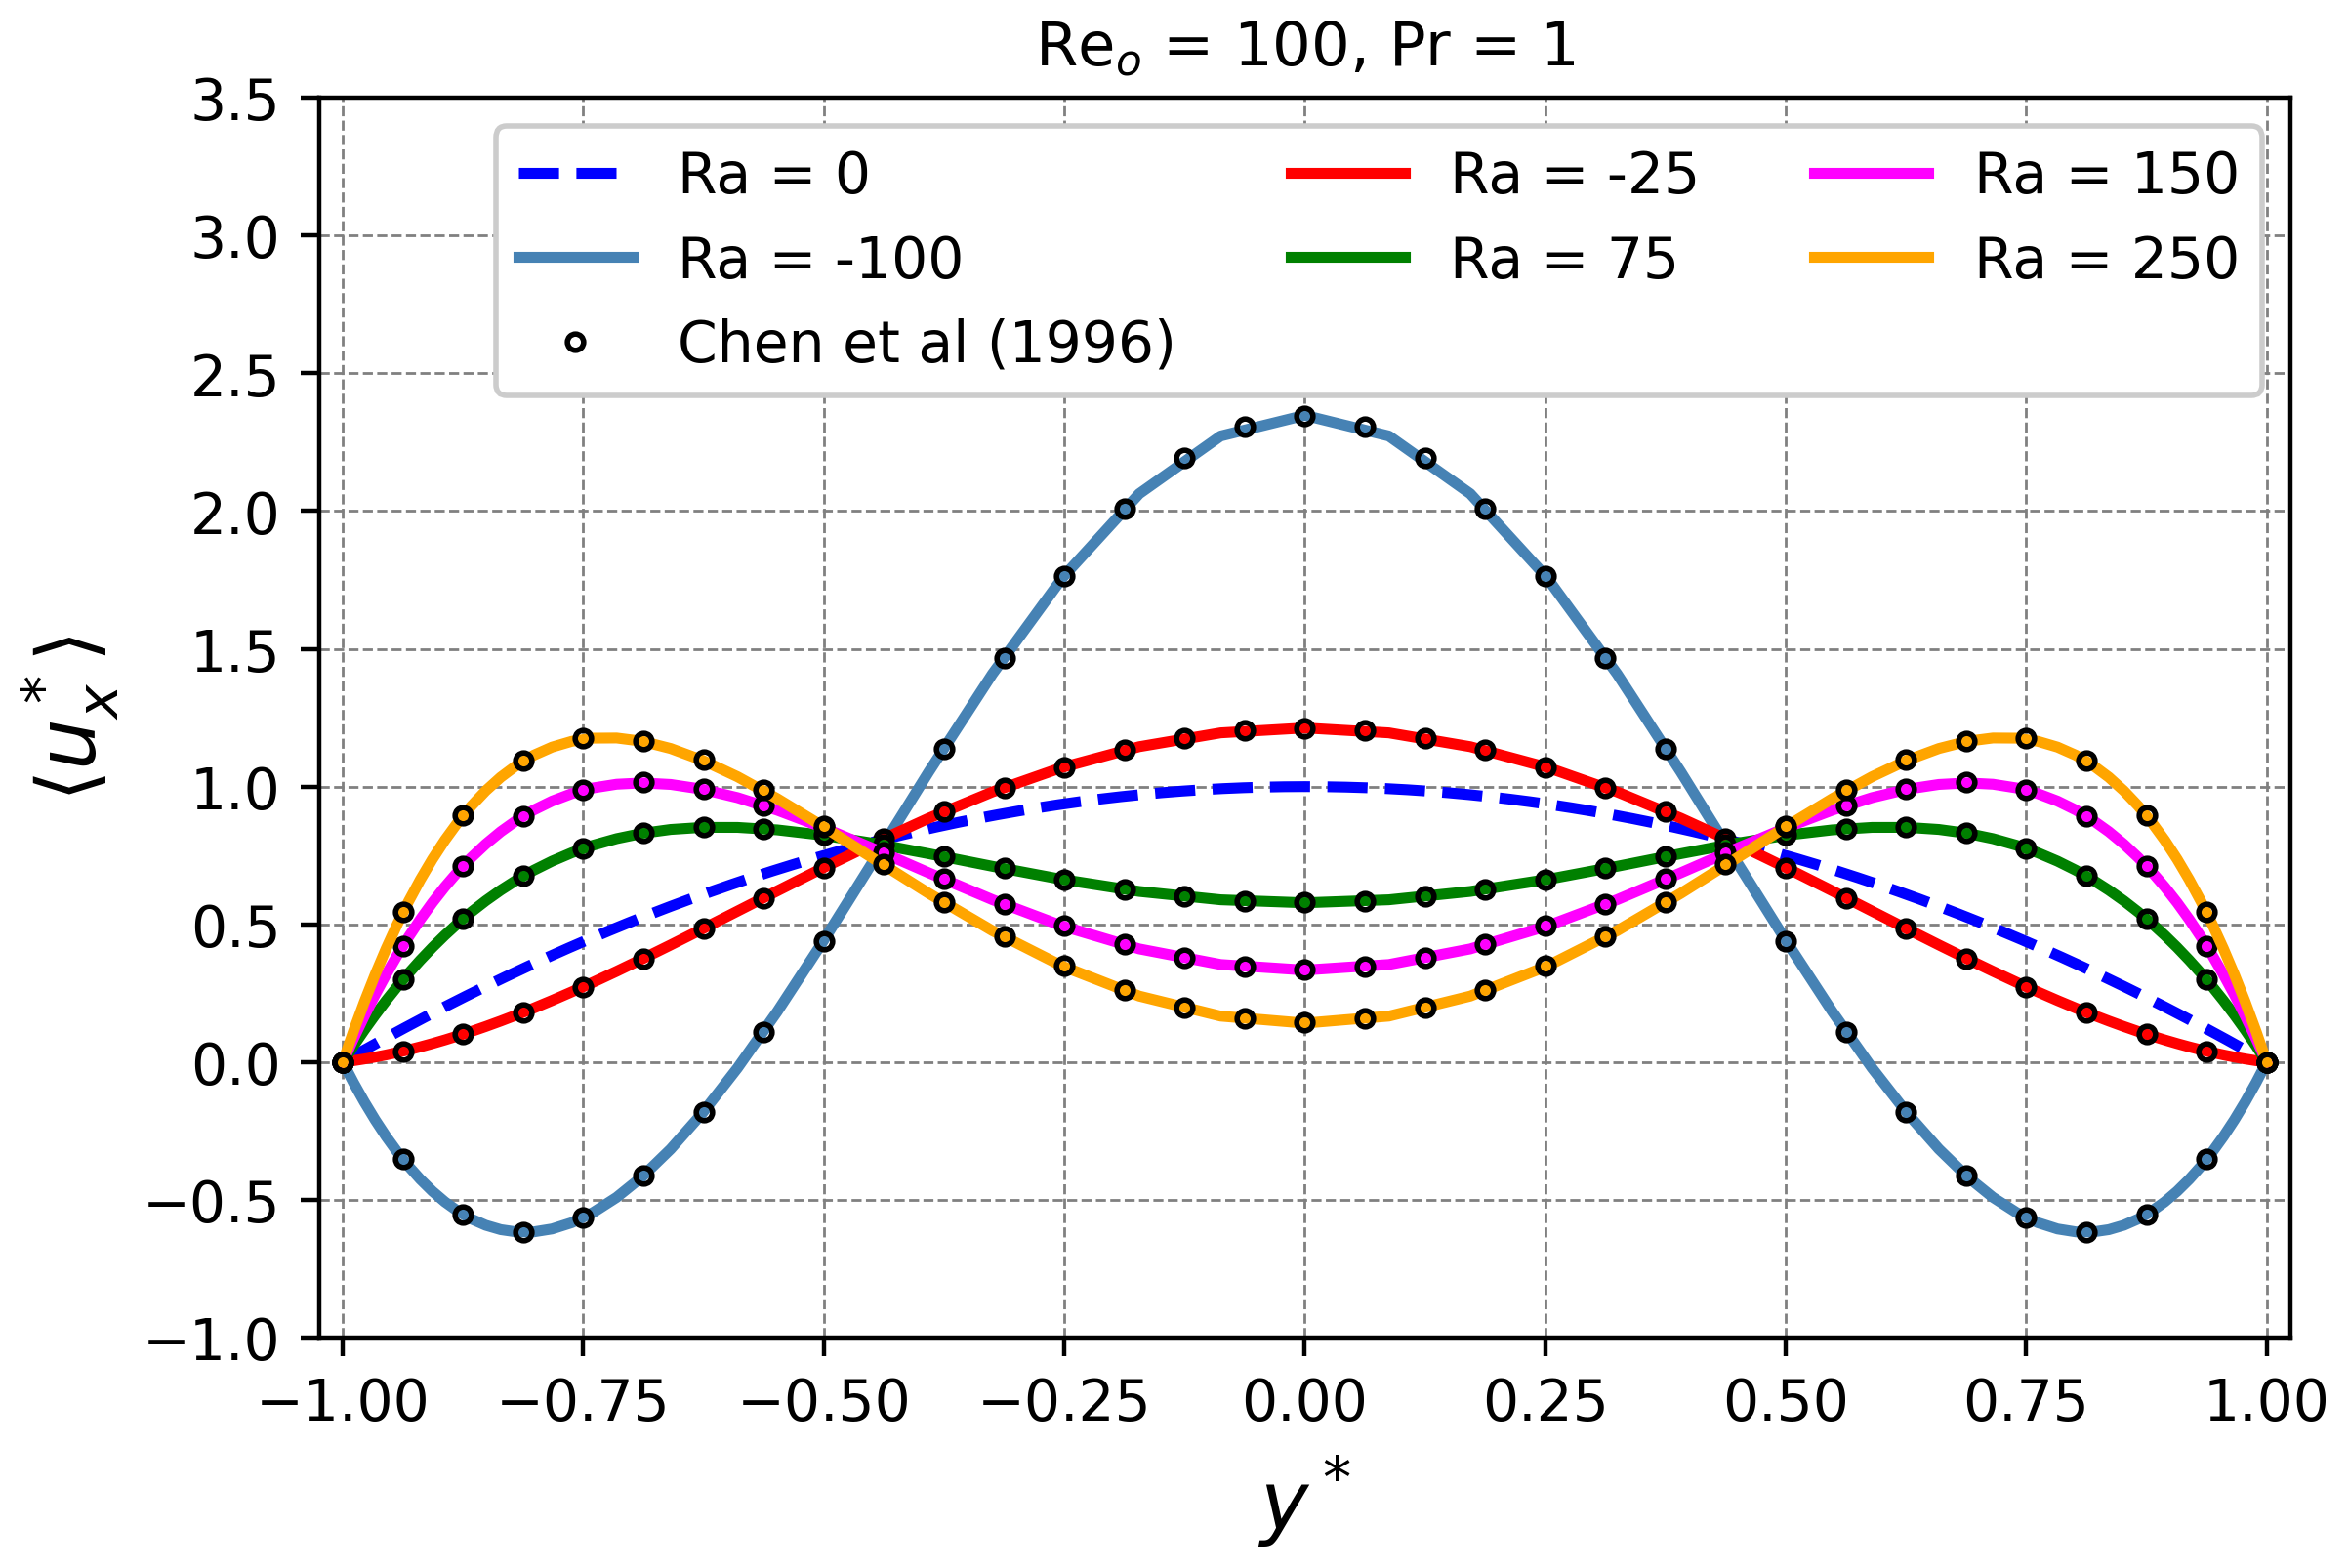
\includegraphics[width=0.5\textwidth]{figures/cap4/laminar/ux_mean.png}
    \label{fig:chen-ux}}  
    \subfloat[]{
    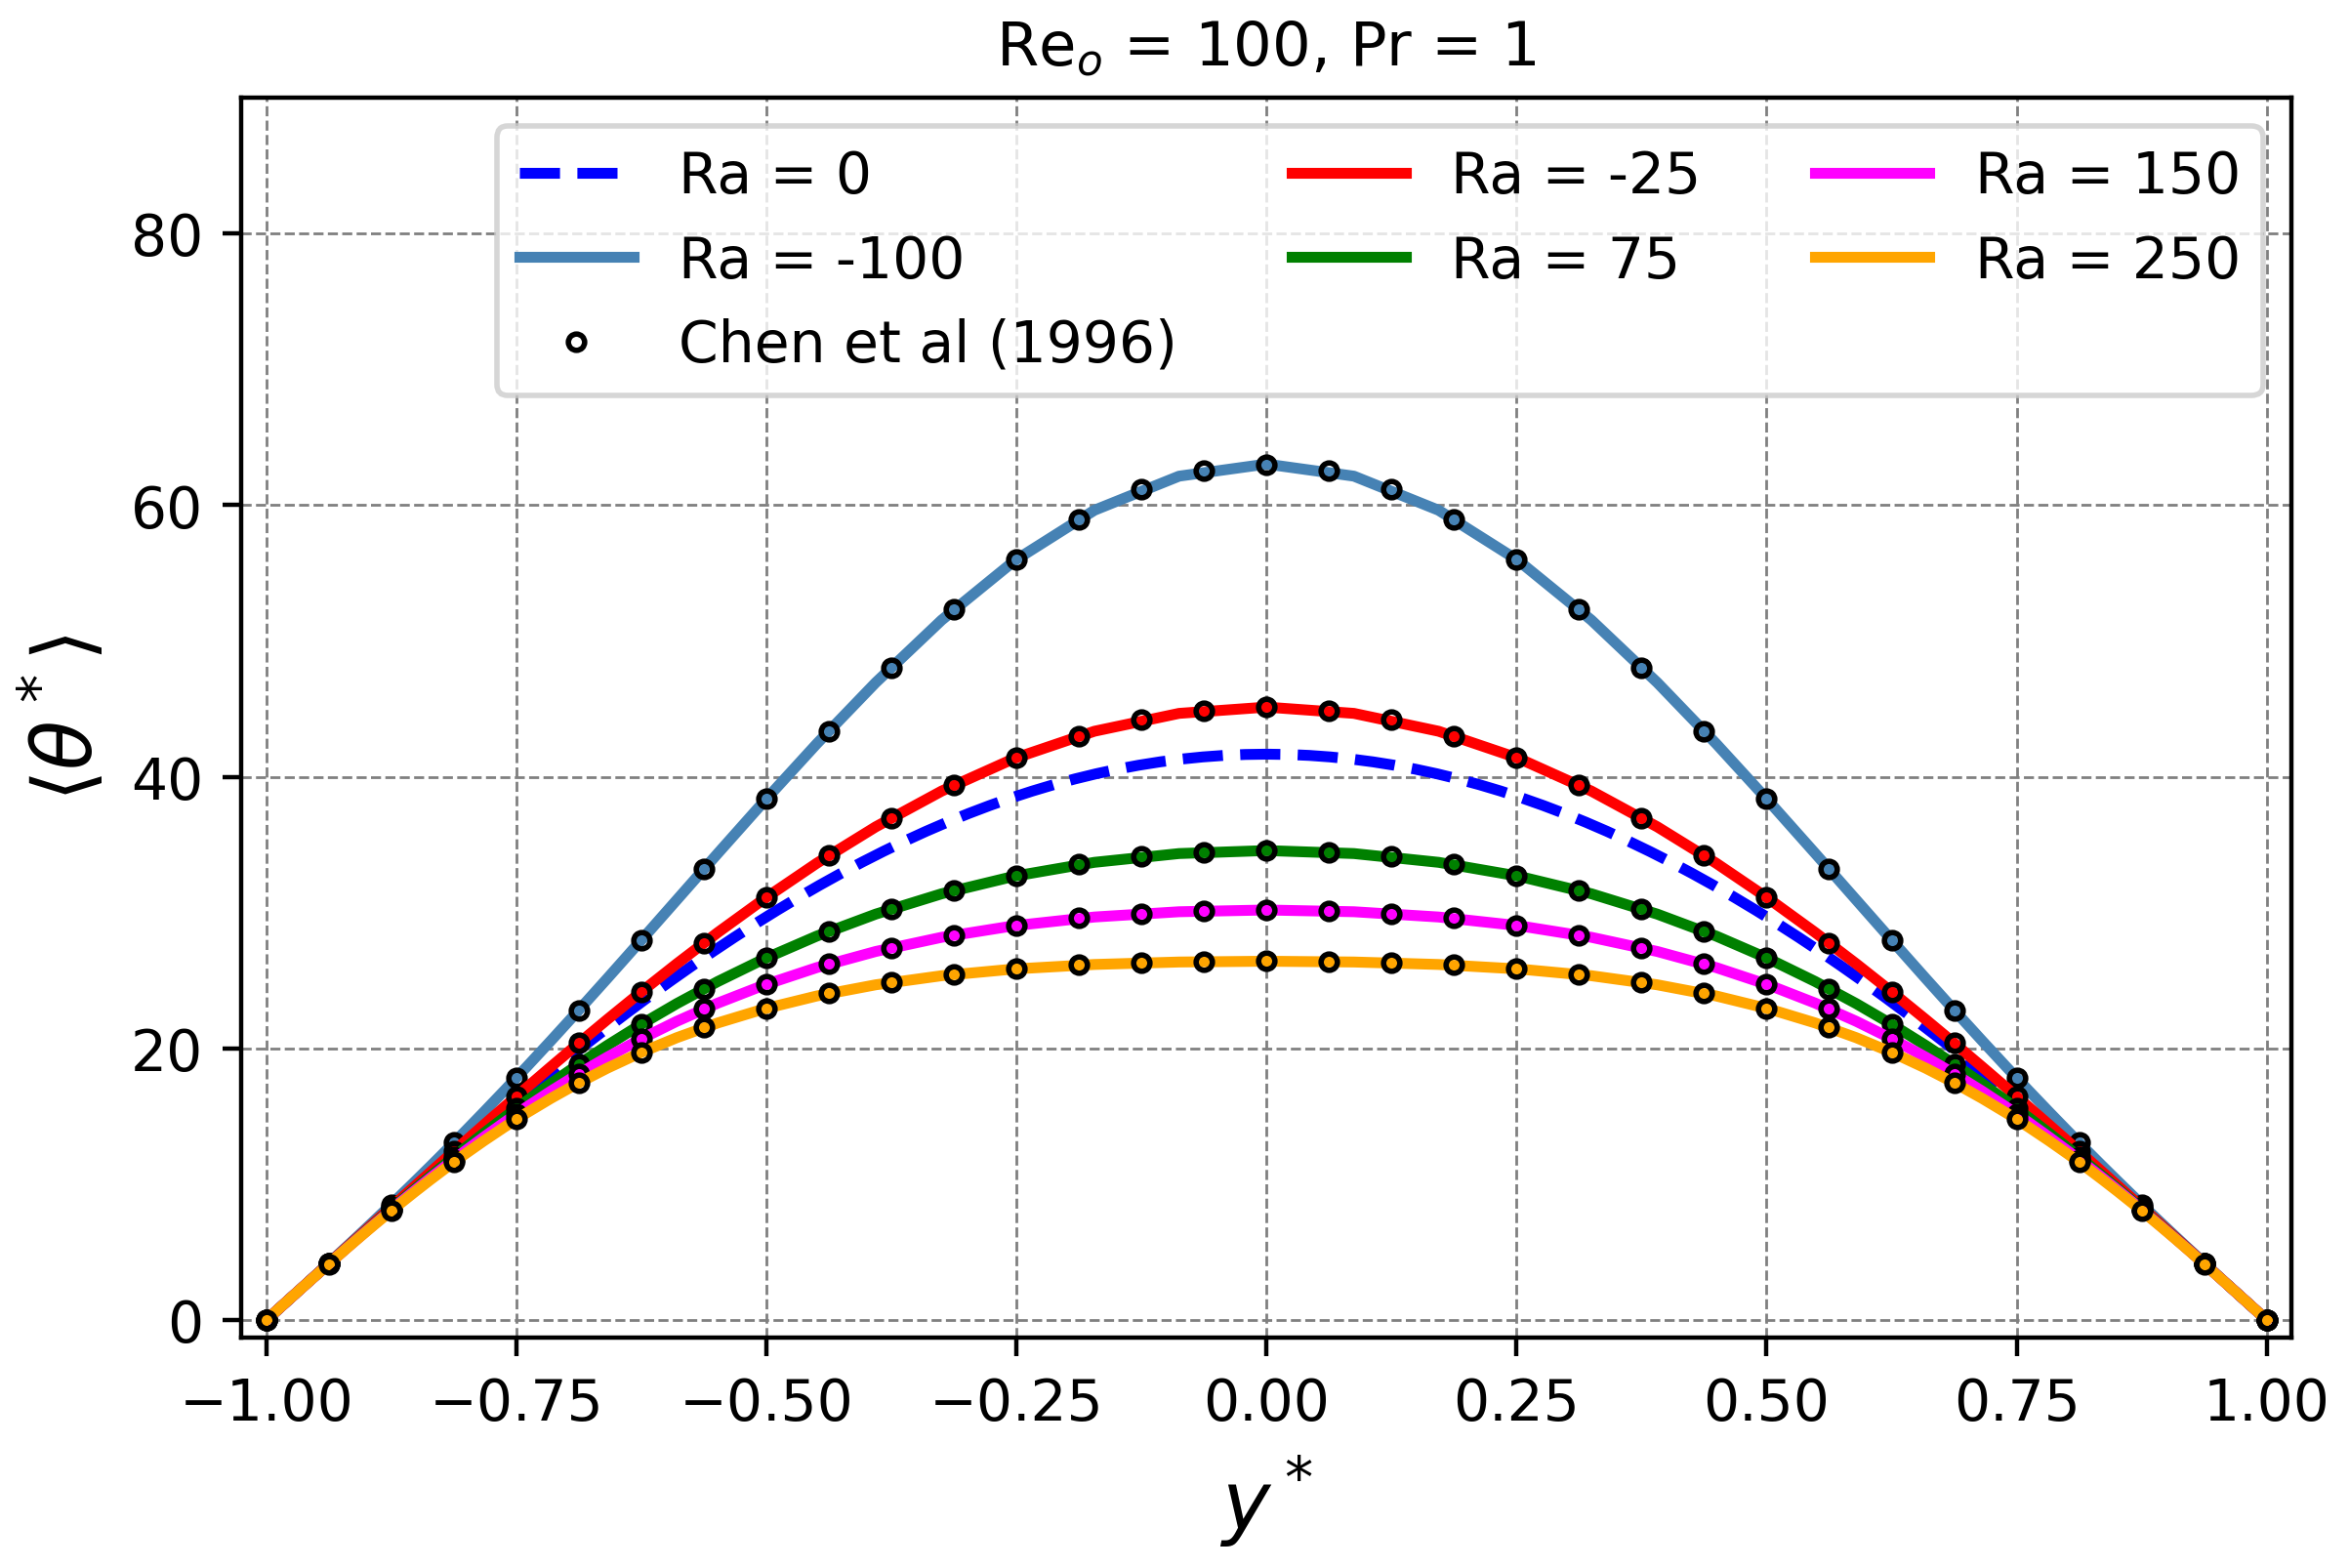
\includegraphics[width=0.5\textwidth]{figures/cap4/laminar/theta_mean.png}
    \label{fig:chen-theta}}  
 \caption{Perfiles de: \textbf{(a)} velocidad y \textbf{(b)} temperatura, considerando distintos casos en régimen laminar con convección mixta.} 
 \label{fig:chen-profiles}
\end{figure}


\subsection{Situación IV. Canal turbulento en convección mixta con $\Delta T$ constante entre paredes.}

\textit{\textbf{Observación inicial}: al momento de realizar las simulaciones para validar la implementación del término de fuerza boyante en XC3D, no se encontraban disponibles en la literatura datos de referencia. En particular, faltaban datos para canales rectangulares con flujo turbulento en régimen de convección mixta, ascendente o descendente, y con flujo de calor impuesto en las paredes. La alternativa disponible utilizada fue el trabajo de Guo \textit{et al.} \cite{guo2022direct} basado en un sistema físico conceptualmente diferente\footnote{En ese sentido, las ecuaciones de gobierno empleadas en el trabajo de Guo \textit{et al.} son ligeramente diferentes a nuestras ecuaciones de gobierno \ref{eq:gob_system_adim}. Por ejemplo, una diferencia que destaca es que, al considerar paredes isotérmicas a distinta temperatura, el término fuente en la ecuación de energía es nulo.} (paredes isotérmicas a distinta temperatura). Más recientemente, tomamos conocimiento del trabajo de Zhou \textit{et al.} \cite{zhou2024direct} que presenta datos DNS con las mismas condiciones de borde empleadas en este trabajo.}


\begin{figure}[H]
 \centering
  \subfloat[]{
    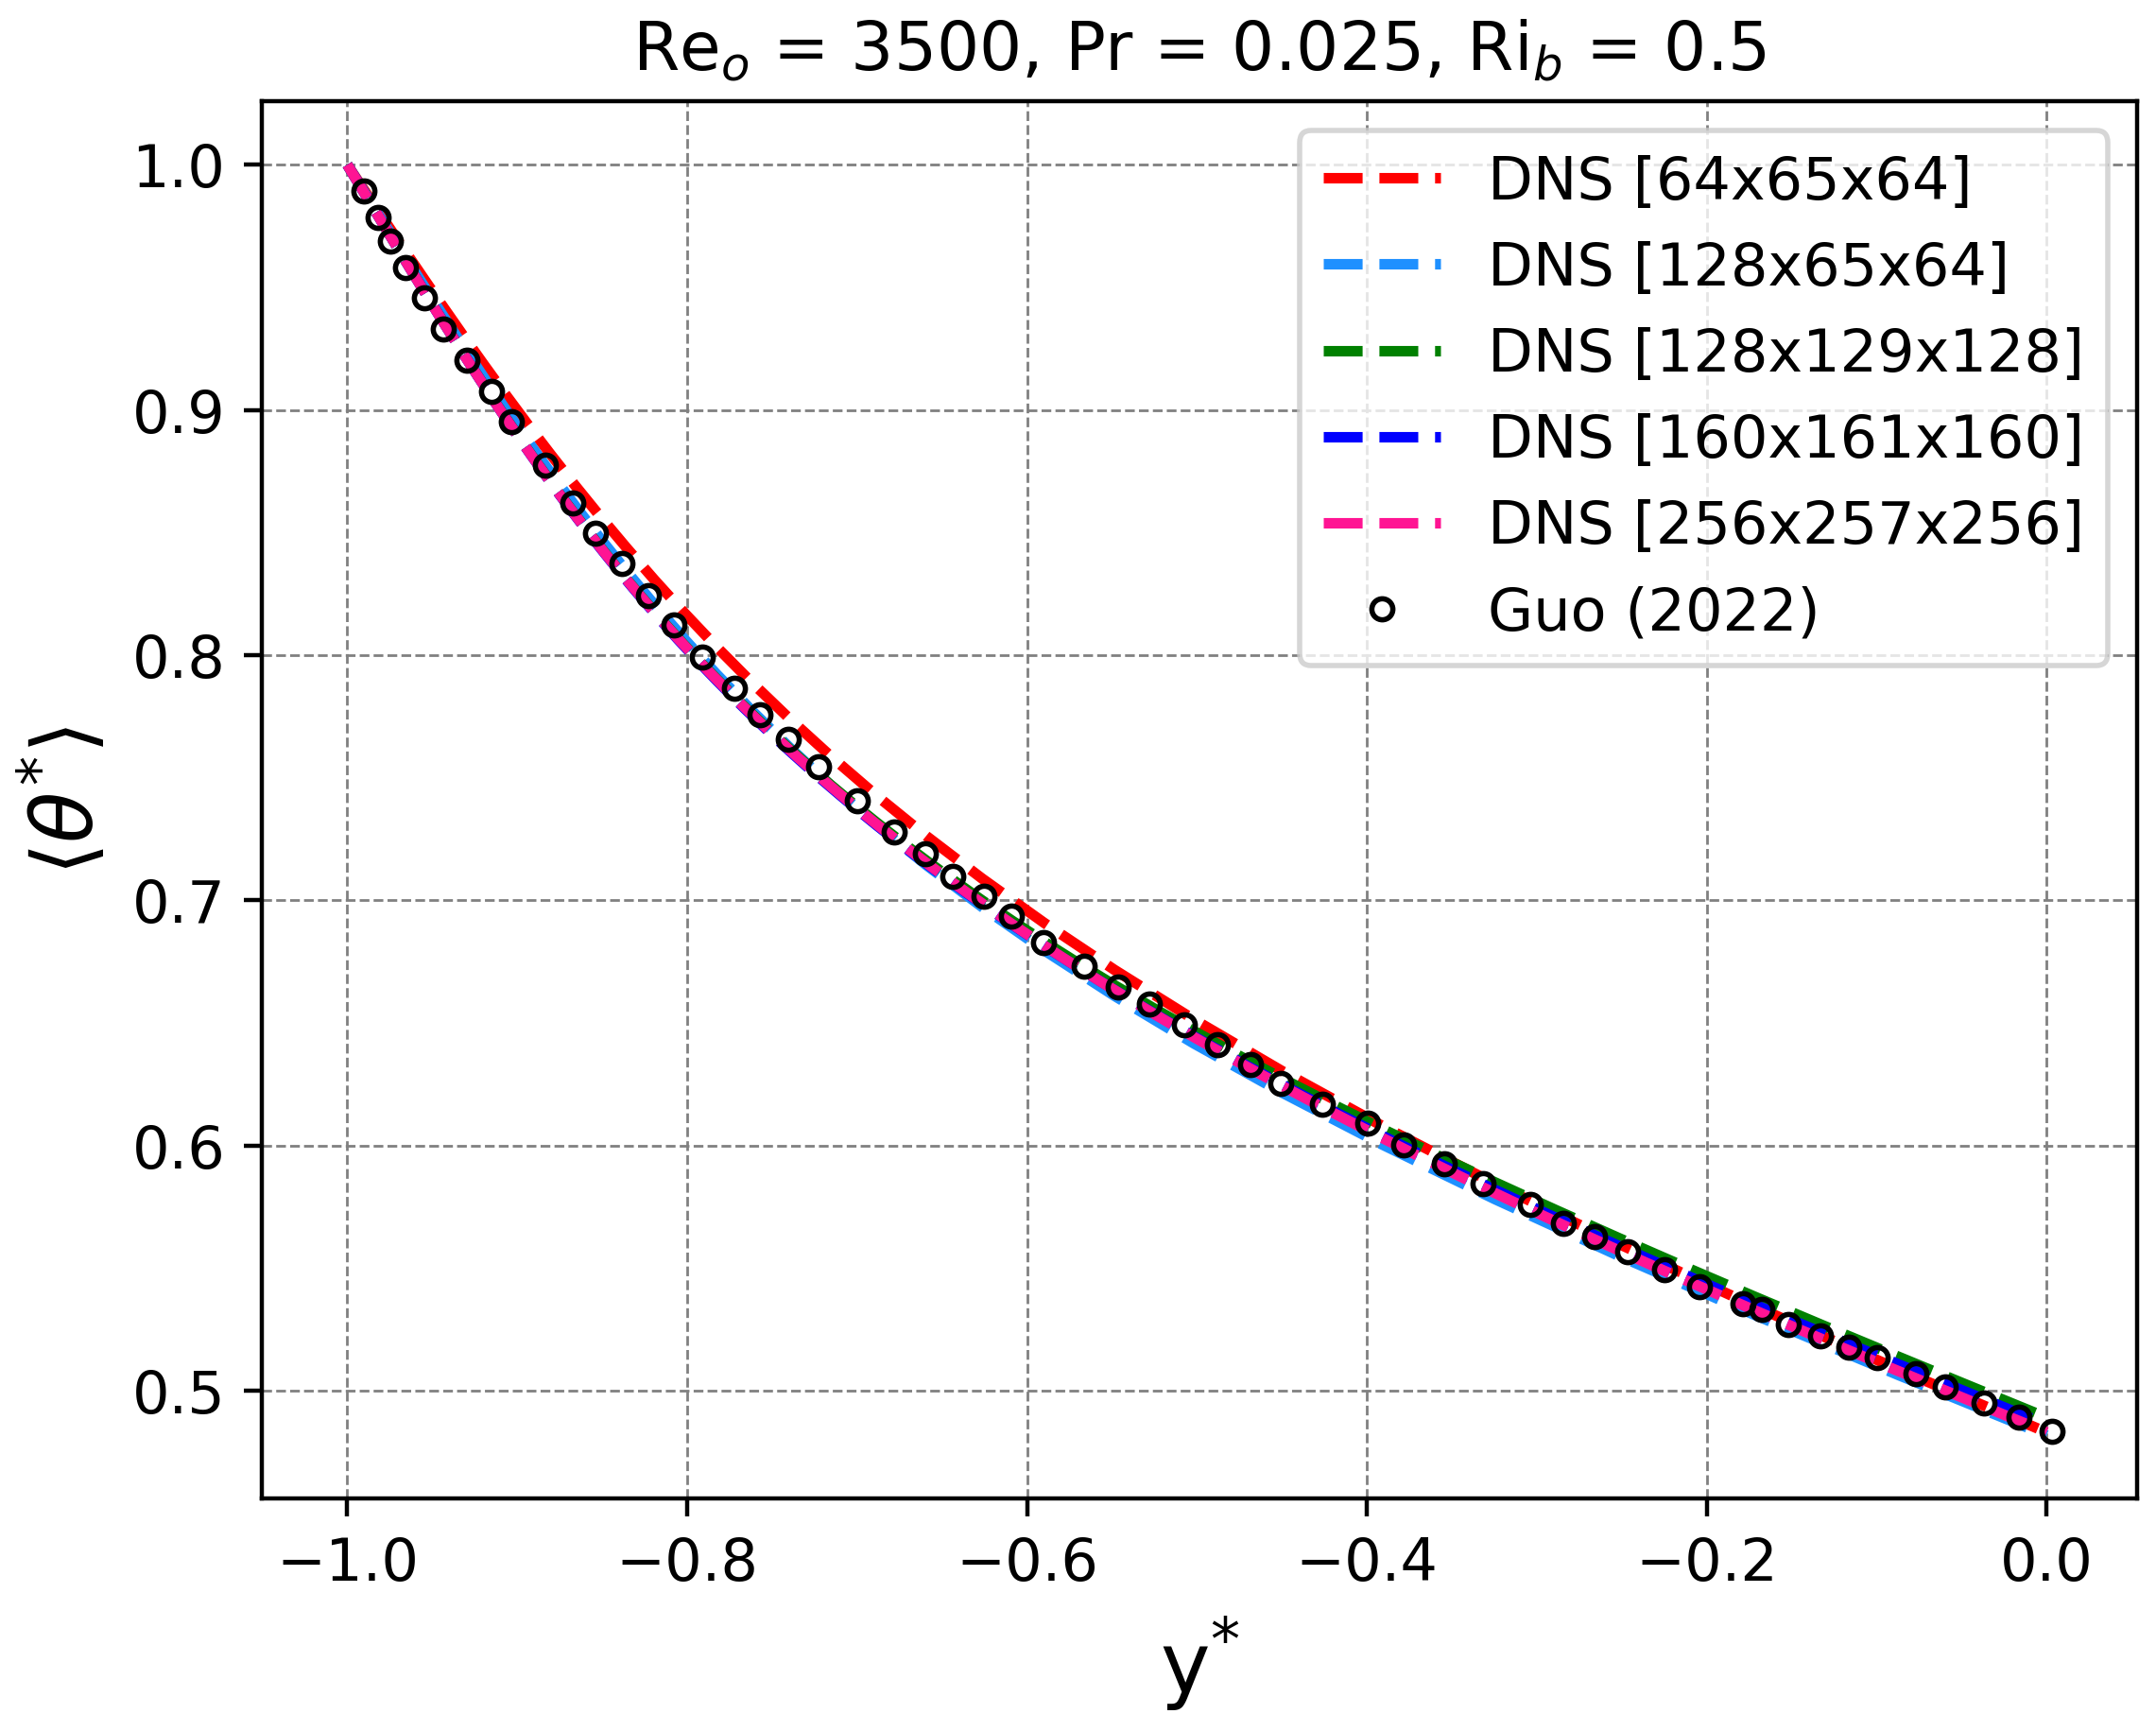
\includegraphics[width=0.49\textwidth]{figures/cap4/guo/Rib05/mct_theta.png}
   		\label{fig:guo-05-theta}}  
    \subfloat[]{
    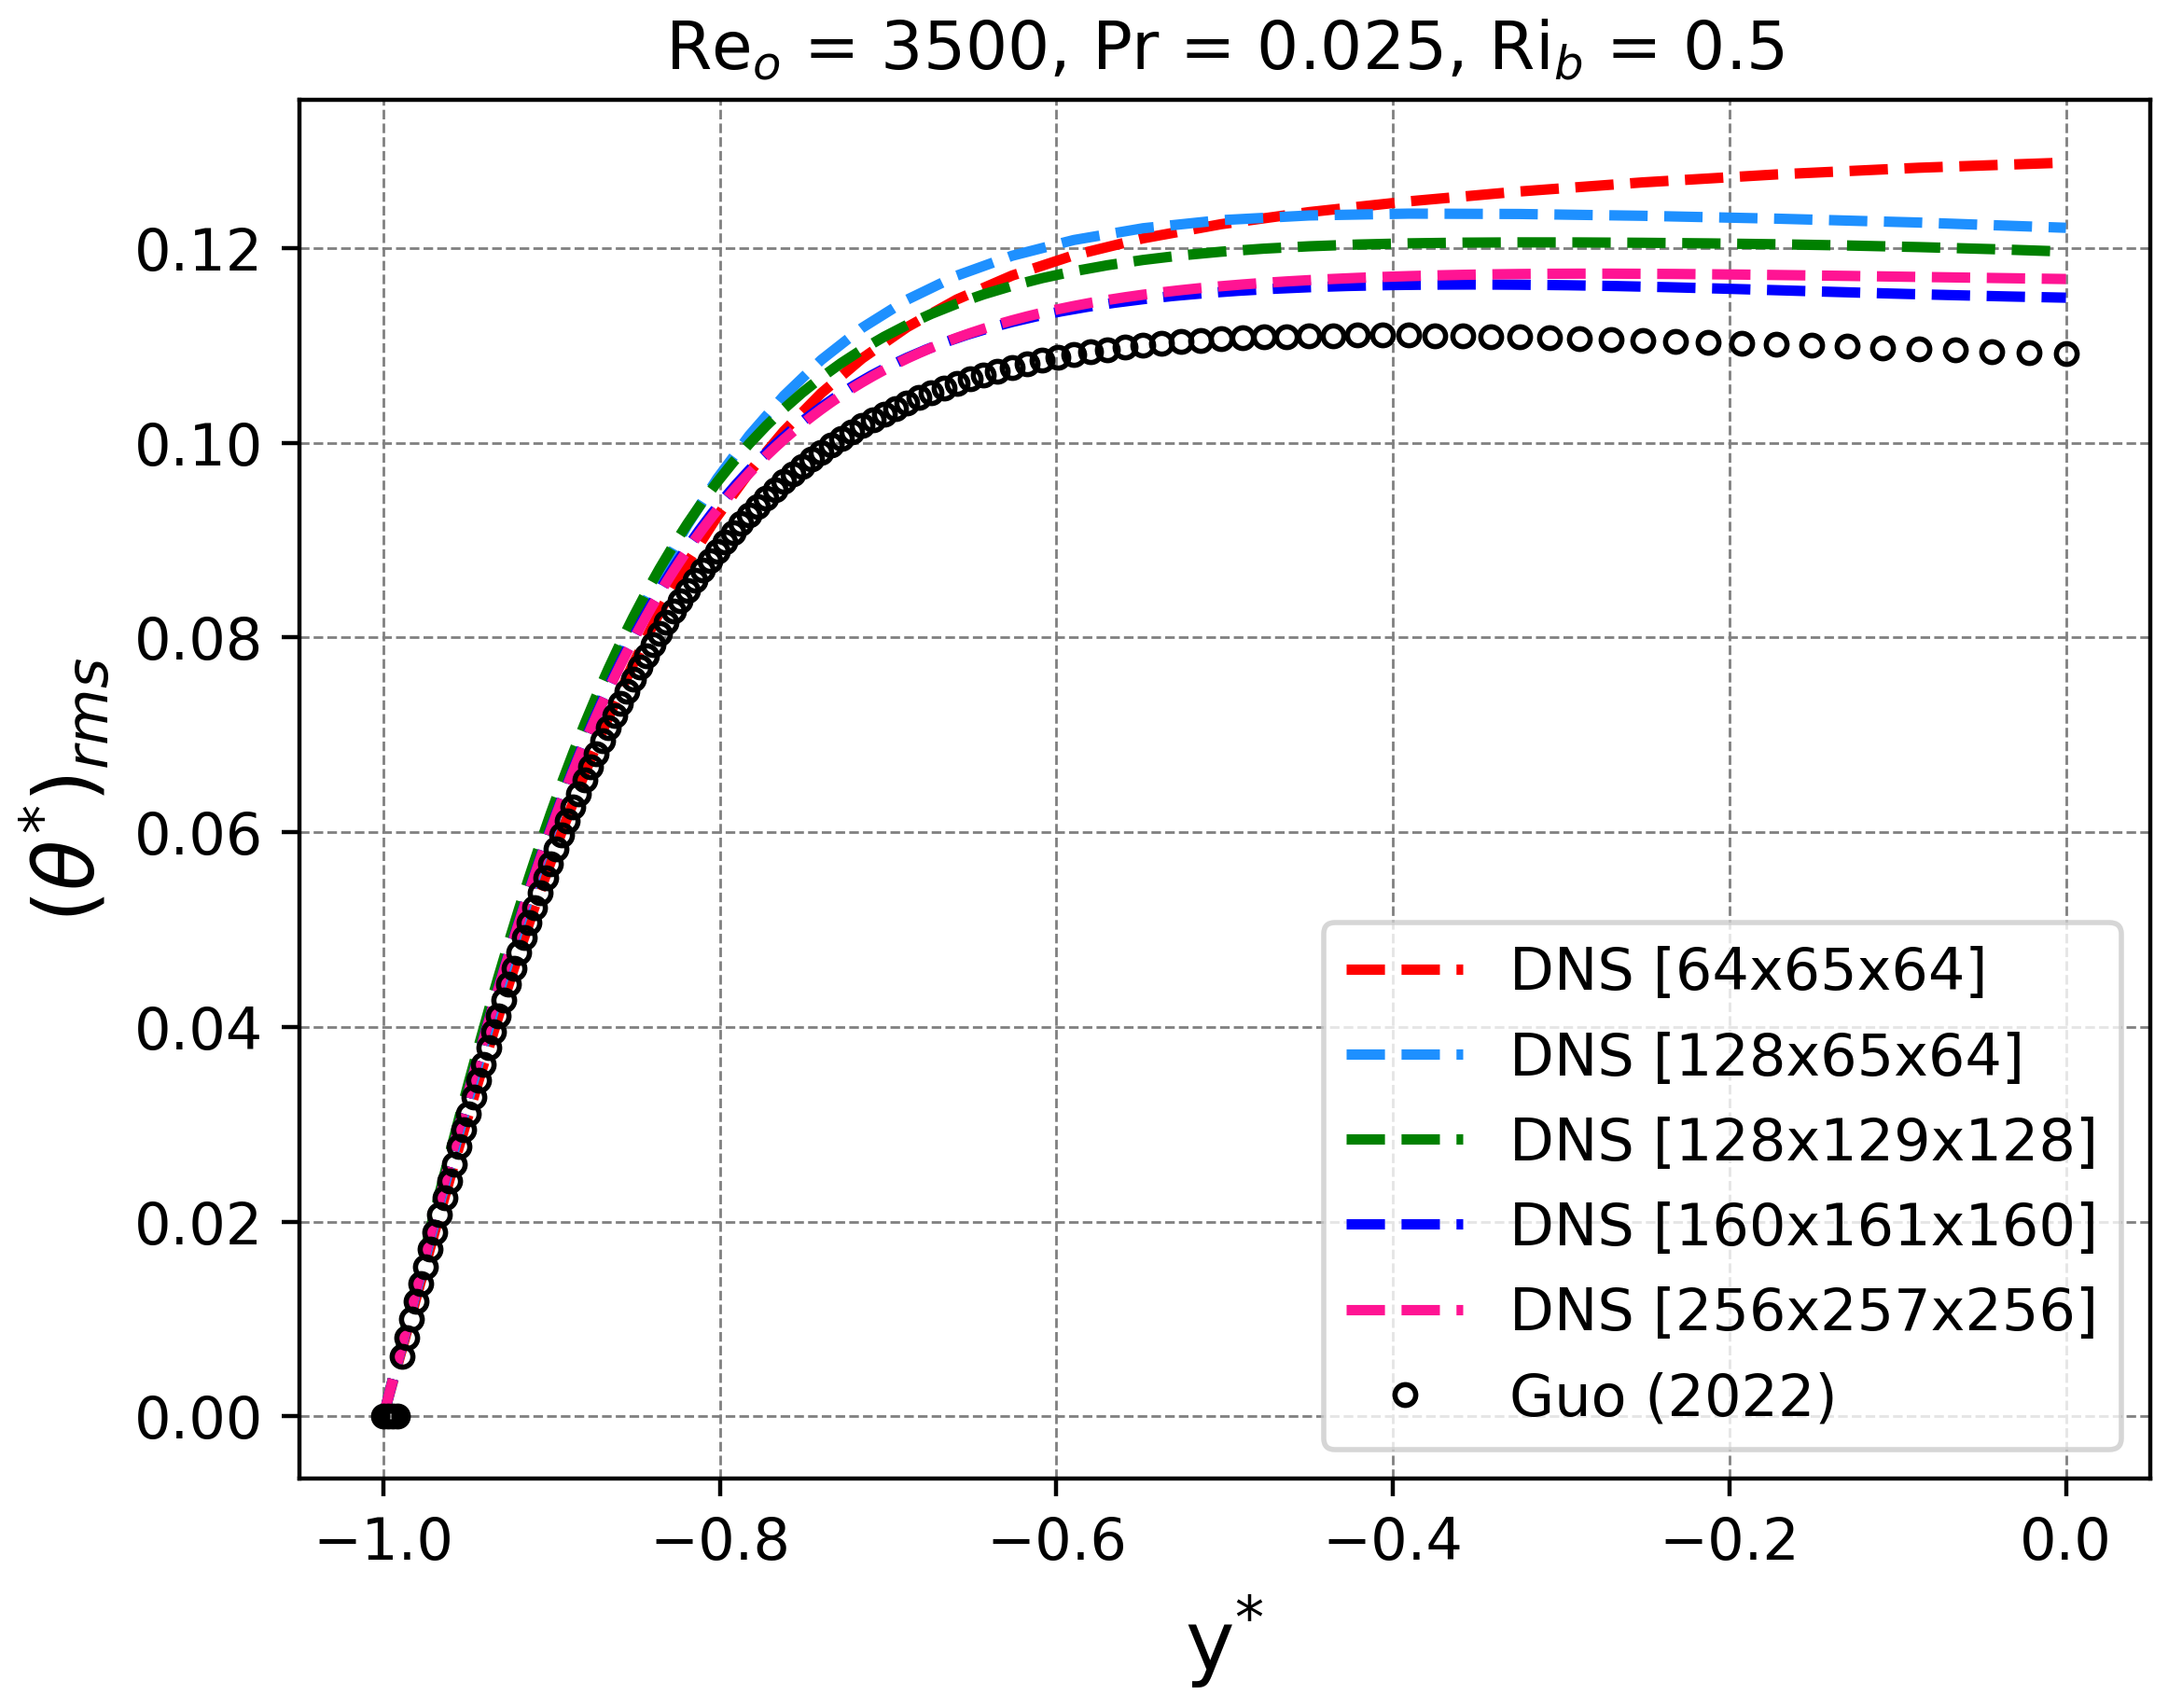
\includegraphics[width=0.49\textwidth]{figures/cap4/guo/Rib05/mct_thetap_rms.png}
  		\label{fig:guo-05-theta-rms}}  

  \subfloat[]{
    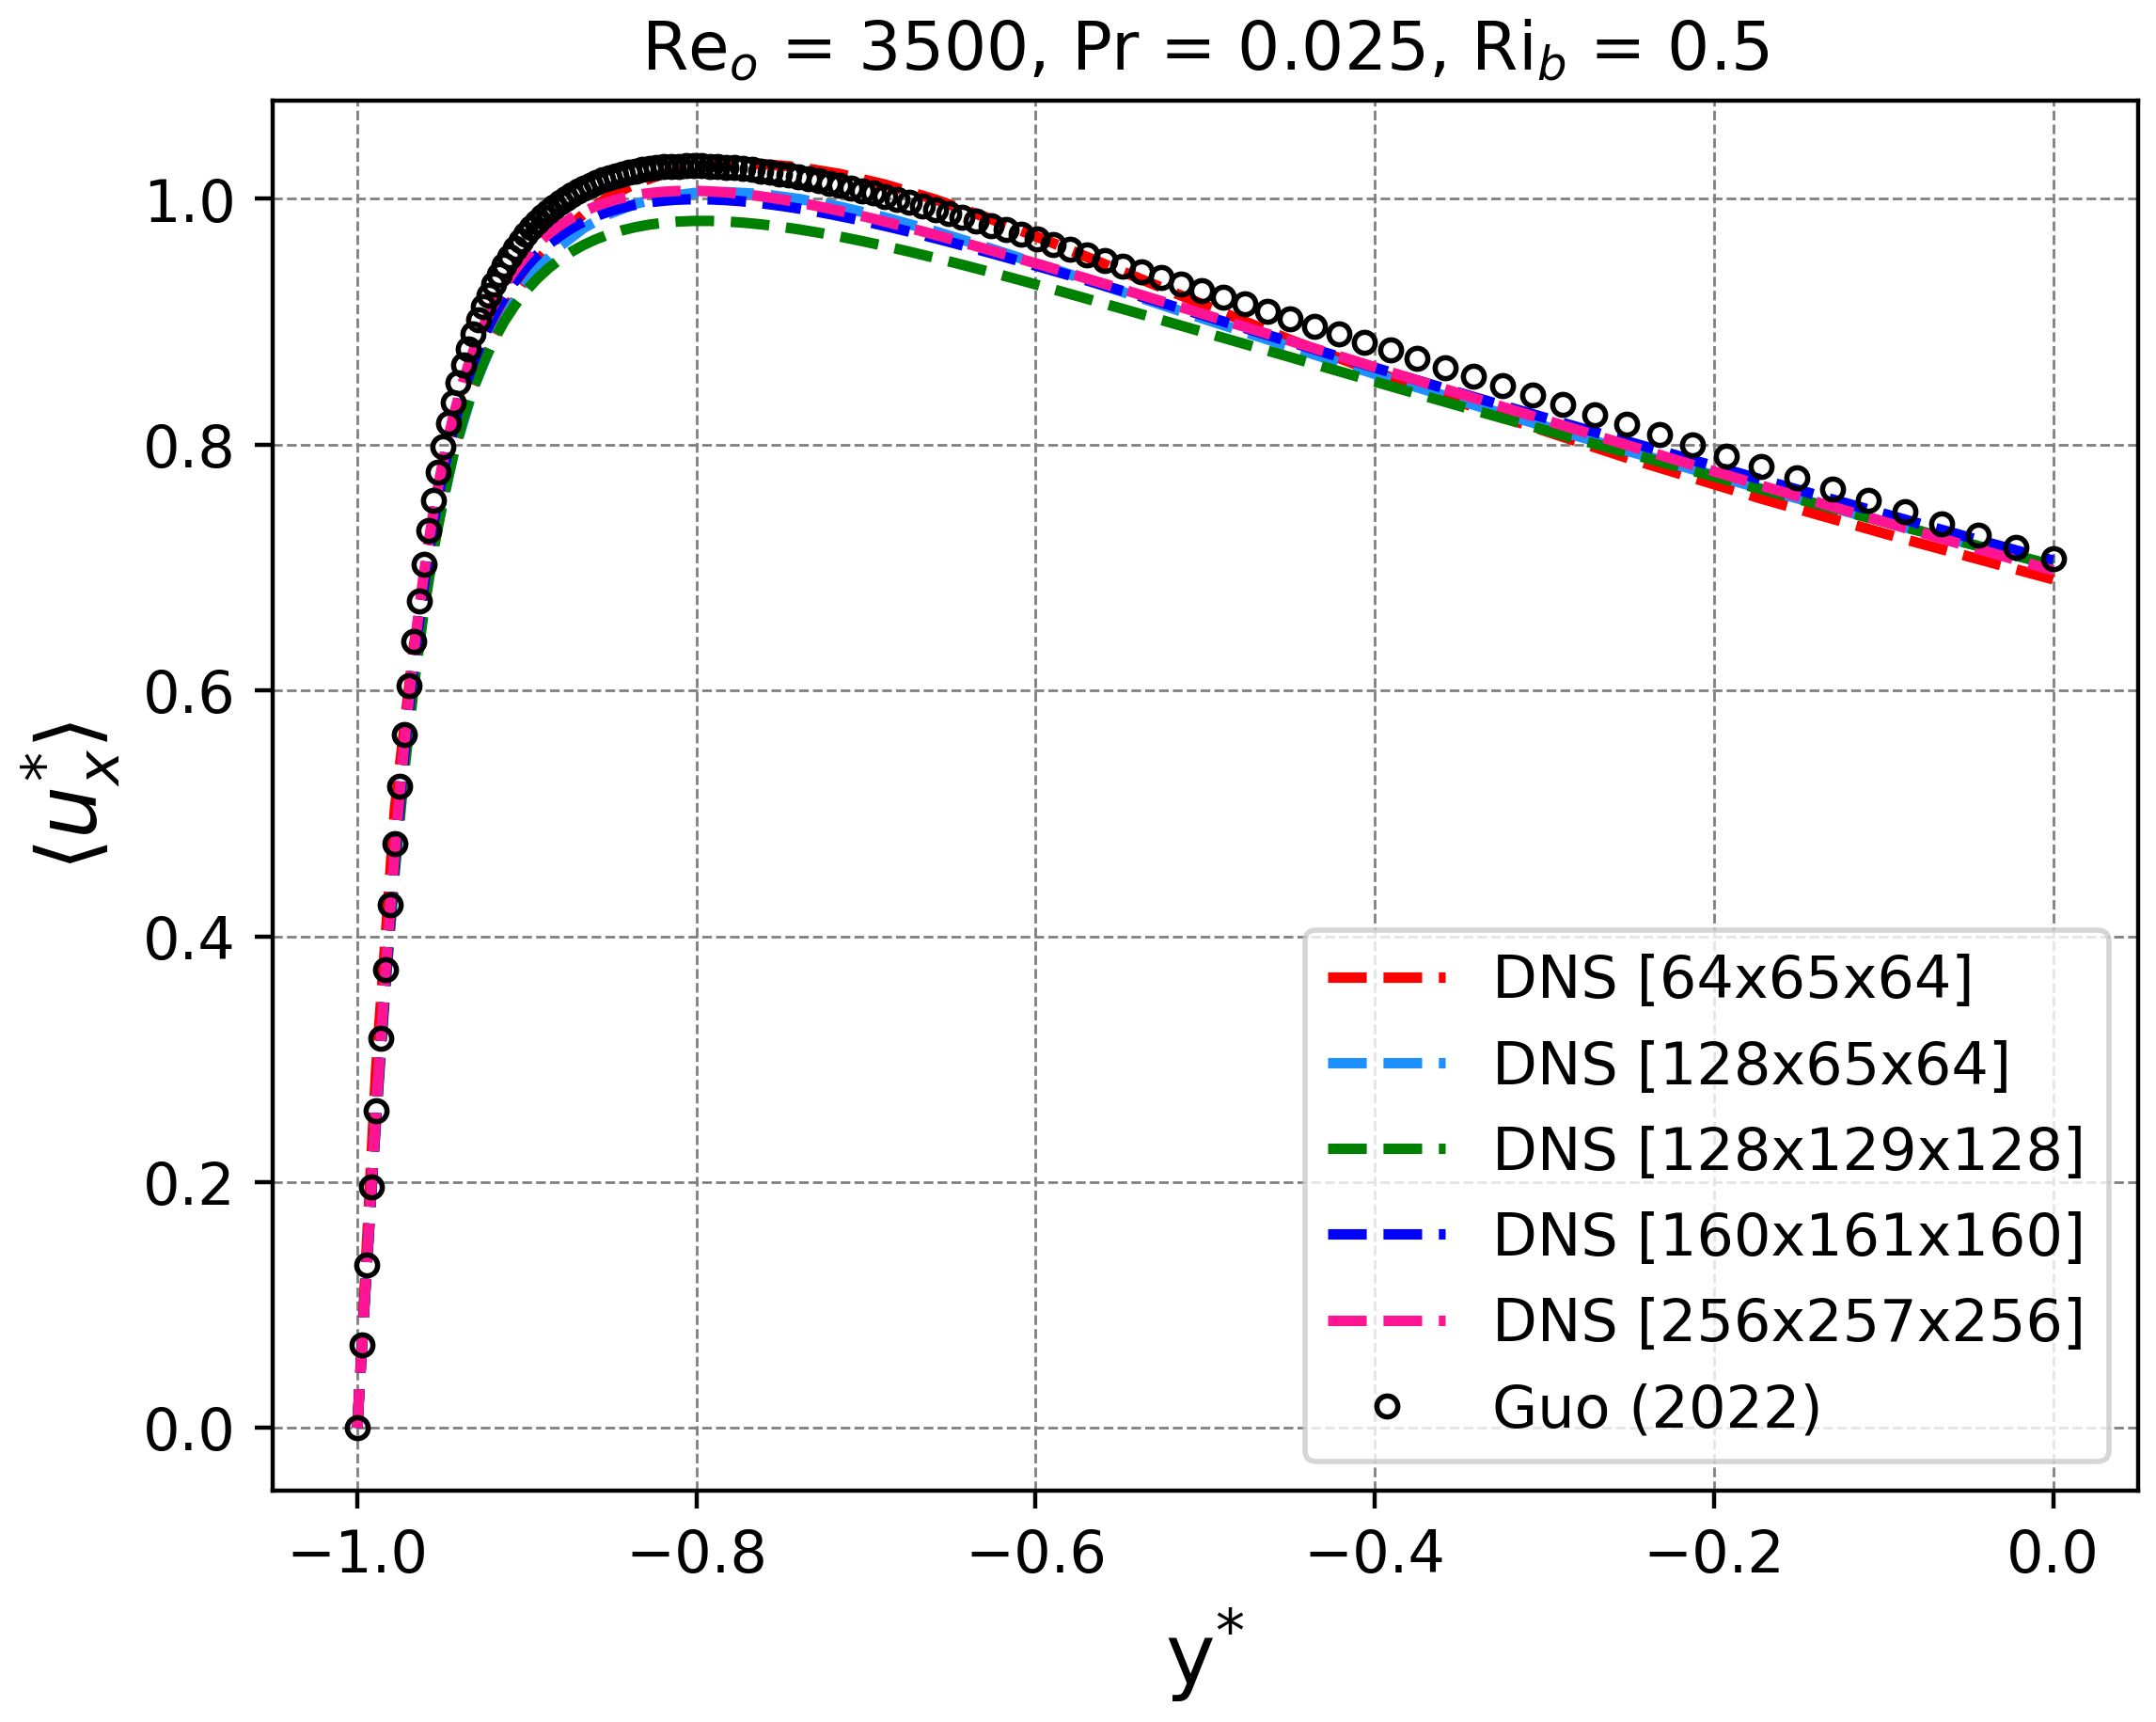
\includegraphics[width=0.49\textwidth]{figures/cap4/guo/Rib05/mct_upmean.png}
   		\label{fig:guo-05-ux}}  
    \subfloat[]{
    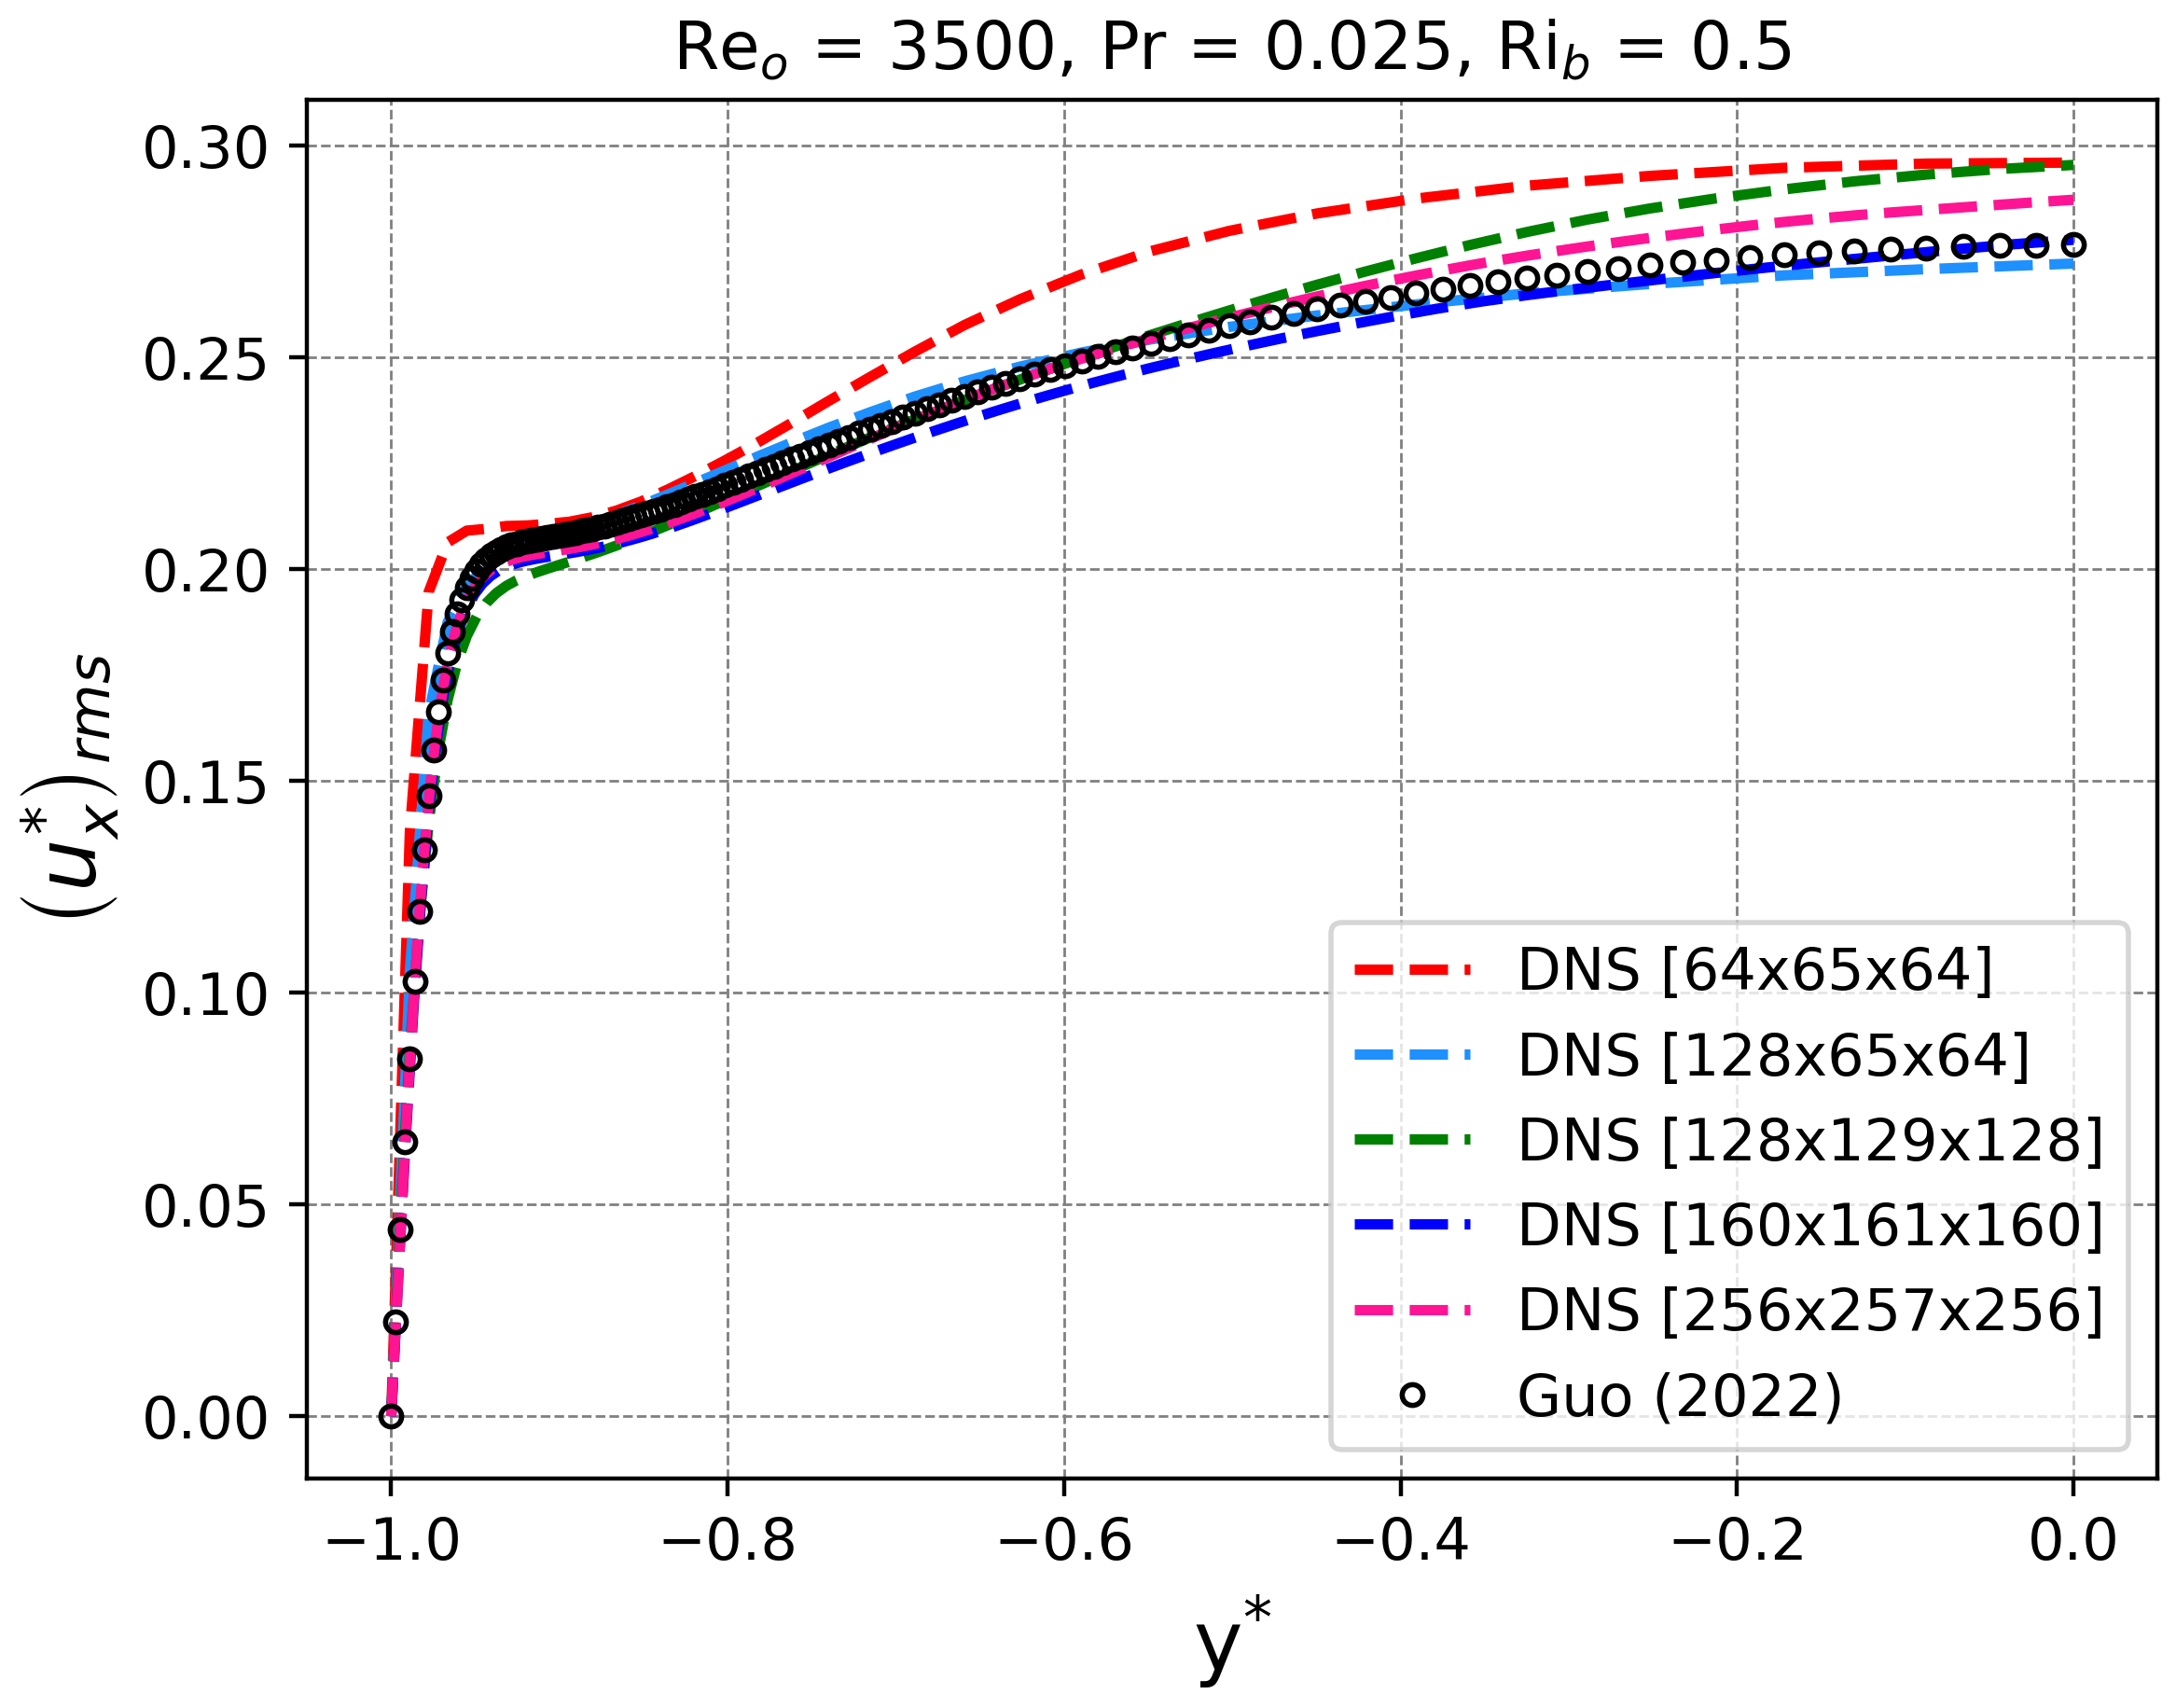
\includegraphics[width=0.49\textwidth]{figures/cap4/guo/Rib05/mct_uprms.png}
    	\label{fig:guo-05-ux-rms}}  

  \subfloat[]{
    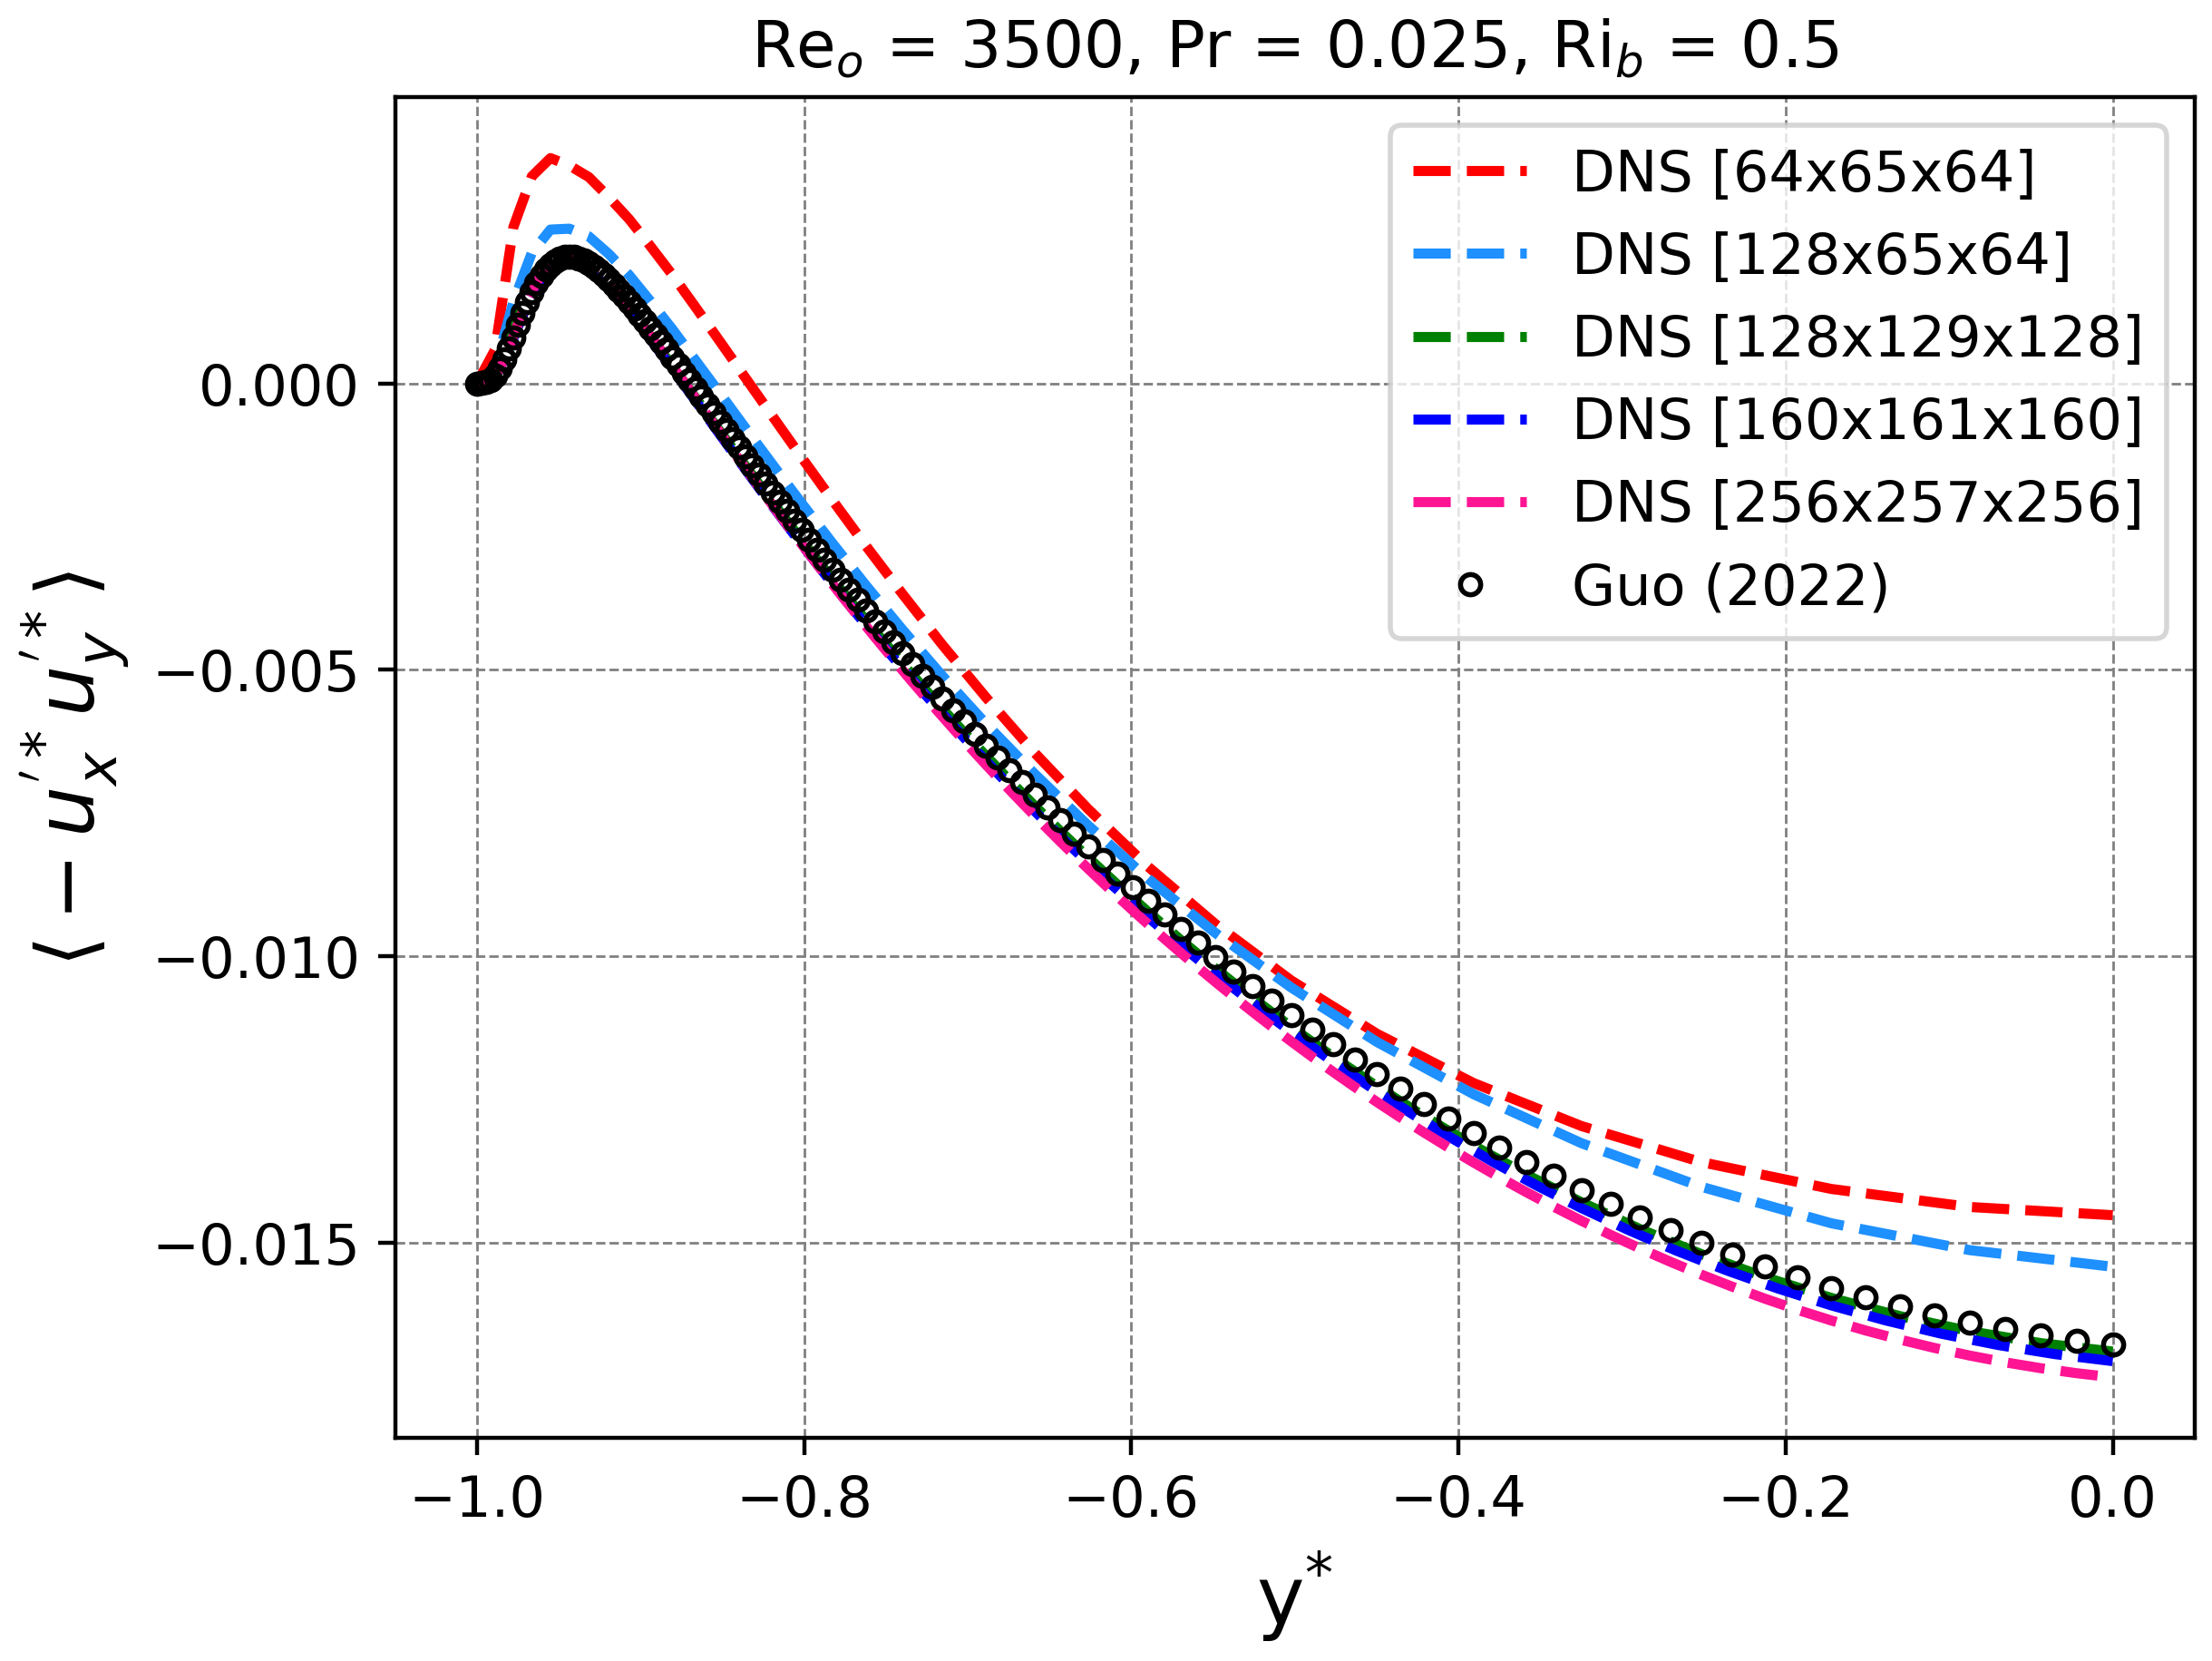
\includegraphics[width=0.49\textwidth]{figures/cap4/guo/Rib05/mct_up_vp.png}
    	\label{fig:guo-05-uxuy}}  
    \subfloat[]{
    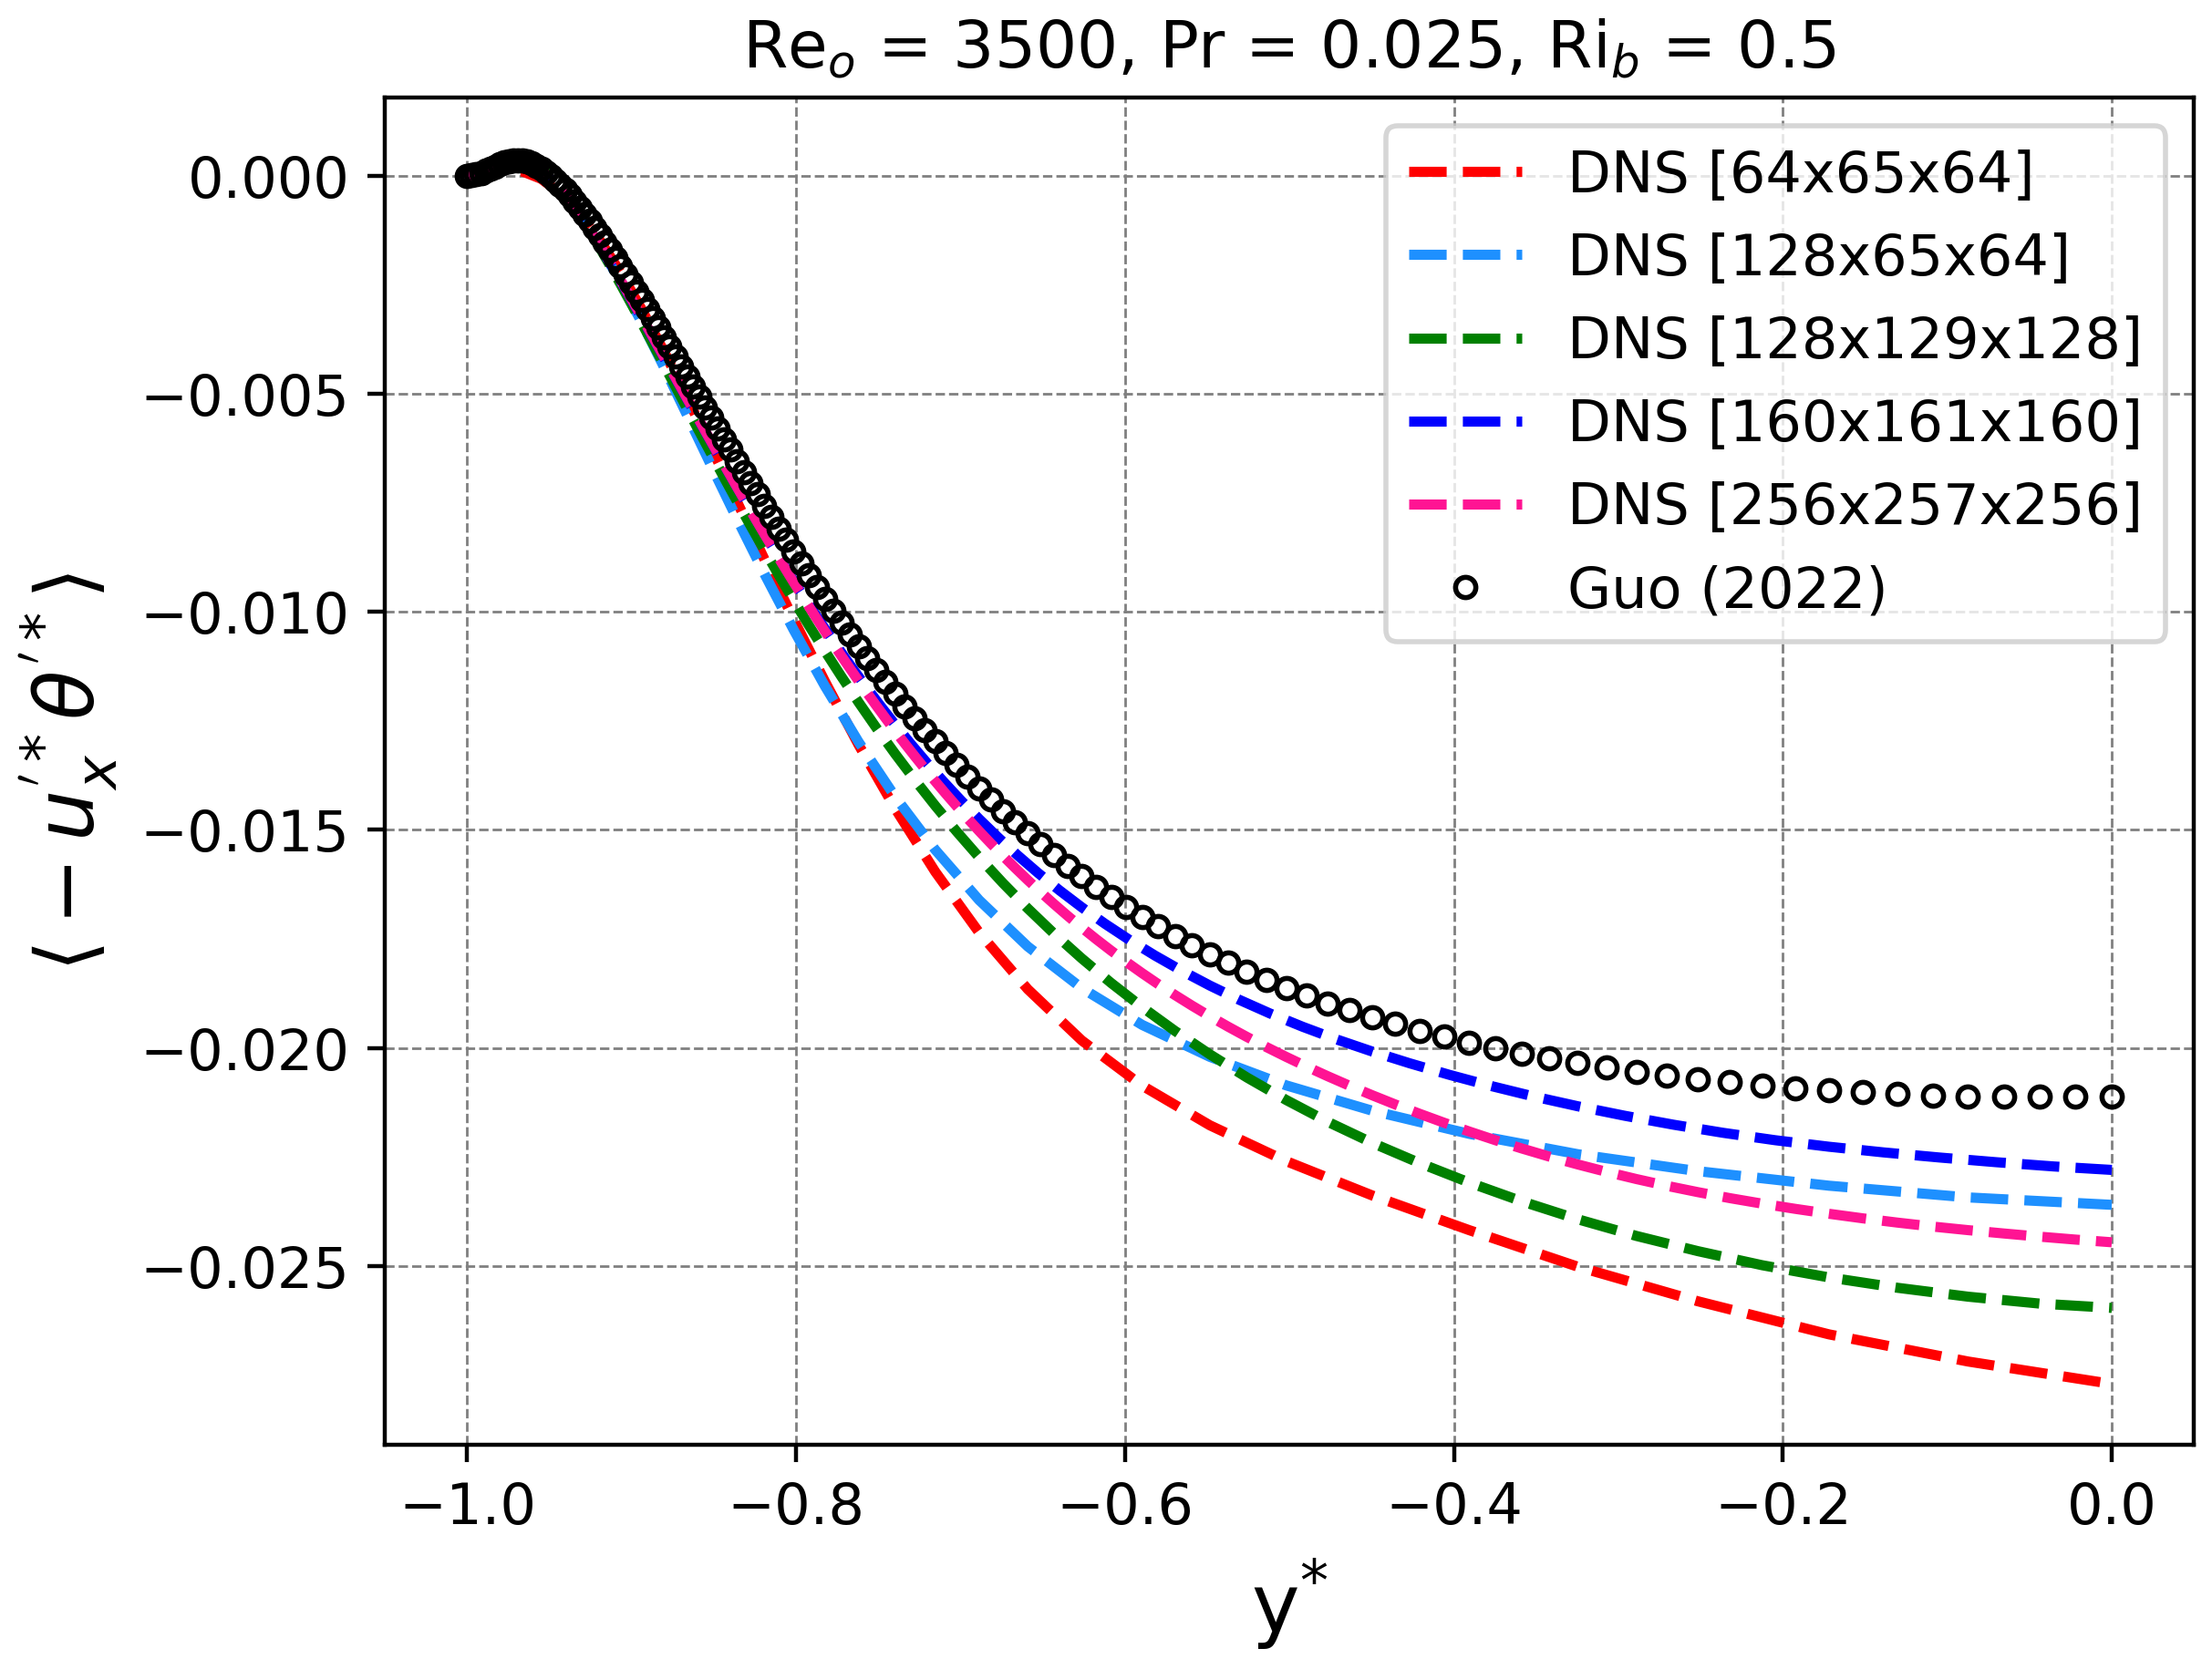
\includegraphics[width=0.49\textwidth]{figures/cap4/guo/Rib05/mct_up_thetap.png}
    	\label{fig:guo-05-ux-theta}}  
 \caption{Perfiles de \textbf{(a)} temperatura adimensional media, \textbf{(b)} fluctuaciones RMS de la temperatura adimensional, \textbf{(c)} velocidad media \textit{streamwise}, \textbf{(d)} fluctuaciones RMS de la velocidad \textit{streamwise}, \textbf{(e)} componente $xy$ del tensor de Reynolds, $\langle -u^+_x u^+_y \rangle$, y \textbf{(f)} flujo de calor turbulento en la dirección X, $\langle -u^+_x \theta^+ \rangle$.} 
 \label{fig:guo-05}
\end{figure}

Cuando se tiene en cuenta la fuerza boyante, es decir $\Pi \neq 0$, el término asociado a ella en la ecuación de momento produce un acople entre las ecuaciones de conservación de momento y energía (ecuaciones \ref{eq:gob_system_adim}) y por lo tanto, la parte hidrodinámica del flujo influye en la parte térmica del mismo y viceversa. 

Se realizan simulaciones empleando las mallas M0 - M4 para analizar su convergencia en malla. En este sentido, se consideran los números adimensionales Re$_o$=3500, Pr=0.025 y Ri$_b$=0.5 para tal fin. Las Figuras \ref{fig:guo-05-theta} - \ref{fig:guo-05-ux-theta} exponen, respectivamente, los perfiles de las siguientes magnitudes\footnote{Nótese que solo se representa un semiancho del canal, esto es, $-1 \leqslant y^* \leqslant 0$.}: temperatura adimensional, fluctuaciones de temperatura, velocidad \textit{streamwise}, fluctuaciones de velocidad, componente $xy$ del tensor de Reynolds y flujo de calor turbulento en la dirección $X$. Los datos de magnitudes propias se comparan con aquellos datos obtenidos por Guo \textit{et al.} \cite{guo2022direct}. Las mismas se encuentran expresadas en la forma adimensional: $\mathbf{u^*} = \mathbf{u} / U_b$ y $\theta^* = \theta / \Delta T_{hc}$, siendo $U_b$ la velocidad \textit{bulk} y $\Delta T_{hc}$ la diferencia de temperatura entre las paredes.

Se observa que las Figuras \ref{fig:guo-05-theta} y \ref{fig:guo-05-ux} verifican una buena convergencia en malla de las  magnitudes de primer orden, es decir, perfiles de velocidad media y temperatura media. Sin embargo, se puede identificar por simple observación, que las diferencias entre nuestras mallas M3 y M4 son, en algunas posiciones del canal, menores a las diferencias entre los datos de referencia y nuestros datos para M4. Esto sugiere que posteriores refinamientos no producirán soluciones más próximas a la referencia. 

Adicionalmente, al comparar magnitudes de segundo orden asociadas a la temperatura adimensional, como la fluctuación de temperatura (Figura \ref{fig:guo-05-theta-rms}) o el flujo de calor turbulento (Figura \ref{fig:guo-05-ux-theta}), se puede destacar una clara diferencia cuantitativa entre nuestros datos para M4 y la referencia en algunas posiciones del semiancho, como por ejemplo en el centro del canal. Por otro lado, en las magnitudes de segundo orden asociadas a la velocidad como las fluctuaciones (Figura \ref{fig:guo-05-ux-rms}) o la componente $xy$ de la tensión de Reynolds (Figura \ref{fig:guo-05-uxuy}), la discrepancia cuantitativa entre los datos obtenidos con M4 y aquellos de referencia sigue siendo apreciable en el centro del canal; sin embargo, es menor que la registrada para la temperatura.

Se especula que los aspectos más relevantes para explicar las diferencias encontradas en los perfiles de las magnitudes de segundo orden, están asociados al tamaño del dominio simulado. Guo \textit{et al.} utilizan un dominio ampliamente mayor ($L_x \times L_y \times L_z = 31\text{.}42 \times 2 \times 12\text{.}57$) que el empleado en este trabajo. Debido a la periodicidad en $x$, los puntos del plano medio $x = L_x/2$ están parcialmente influidos por los puntos en los planos $x=0$ y $x=L_x$. Dicho de otra manera, estos puntos ``fronterizos'' podrían no encontrarse descorrelacionados. Este hecho no permite capturar con precisión todas las escalas que presenta la solución del problema o hace que la solución numérica aún sea dependiente del tamaño del dominio simulado. Otra cuestión adicional que puede influir, es que Guo \textit{et al.} emplean menor resolución (espaciado mayor) en las direcciones $X$ y $Z$, e idéntico en la dirección $Y$: $(\Delta x^*,\Delta y^*_{\text{max}},\Delta z^*) = (0\text{.}061, 0\text{.}022, 0\text{.}024)$. Por lo tanto, luego de esta discusión y del análisis de los resultados presentados en las Figuras \ref{fig:guo-05-theta} - \ref{fig:guo-05-ux-theta} se considera que las mallas propuestas, M2-M4, producen resultados con una precisión razonable para los objetivos buscados y permiten llevar adelante el trabajo con la capacidad de cálculo existente. 

\paragraph{Elección de malla para simulaciones posteriores.}

En síntesis, los resultados de esta sección muestran que refinar de M2 a M3/M4 no aporta mejoras apreciables a la escala de las figuras. Dado que las magnitudes de interés\footnote{Por ejemplo, el número de Nusselt y/o el factor de fricción de Darcy.} se obtienen a partir de cantidades estadísticas de primer orden, y además, estas mantienen un buen acuerdo con las referencias, \textbf{se adopta la malla M2} para las simulaciones del Capítulo \ref{cap:desarrollado} por representar el mejor compromiso entre precisión y costo computacional.


\section{Segunda Parte: OSMC}

En esta segunda parte se exponen los resultados obtenidos con la herramienta OSMC, la cual genera autovalores y autofunciones basados en teoría de estabilidad lineal presentada en el Capítulo \ref{cap:modelo}. La validación de la herramienta se realiza en dos etapas: 

\begin{itemize}
	\item \textbf{1.} se valida la fiabilidad de los autovalores calculados;
	\item \textbf{2.} se comparan autofunciones obtenidas con casos de referencia;
	%\item \textbf{3.} se realizan simulaciones DNS para un canal de placas paralelas, con flujo de calor constante en las paredes, cuya condición inicial se construye utilizando el autovalor más inestable y su autofunción asociada. Se compara su evolución temporal con aquella obtenida por análisis de estabilidad lineal.
\end{itemize}

\subsection{Autovalores}

Basados en el proyecto integrador de Pablo Szuban \cite{szuban2023}, se emplea la variación de la parte imaginaria del autovalor más inestable\footnote{Esto es: la parte imaginaria de la cota superior del espectro de autovalores calculado con OSMC para un determinado conjunto de parámetros $\lbrace \alpha, \beta, \text{Re}_o, \text{Pr}, \text{Ra} \rbrace$.}, $c_i$, en función del número de onda en la dirección $X$, $\alpha$, para validar los autovalores obtenidos con OSMC. La Figura \ref{fig:eigenval_alpha} muestra $c_i(\alpha)$ para $\mathrm{Re}_o=322$ y $\mathrm{Re}_o=750$, con $\beta=0$ y Pr = 0.7. Los valores de $\mathrm{Ra}$ se seleccionan de modo que $c_i=0$ para algún $\alpha$ dentro del intervalo considerado: $\mathrm{Ra}=32$.$65$ para \linebreak $\mathrm{Re}_o=322$ y $\mathrm{Ra}=37$.$6$ para $\mathrm{Re}_o=750$. Los resultados se comparan con los de Chen y \linebreak Chung \cite{chen1996linear}, observándose un muy buen acuerdo.

\begin{figure}[H]
	 \centering
    	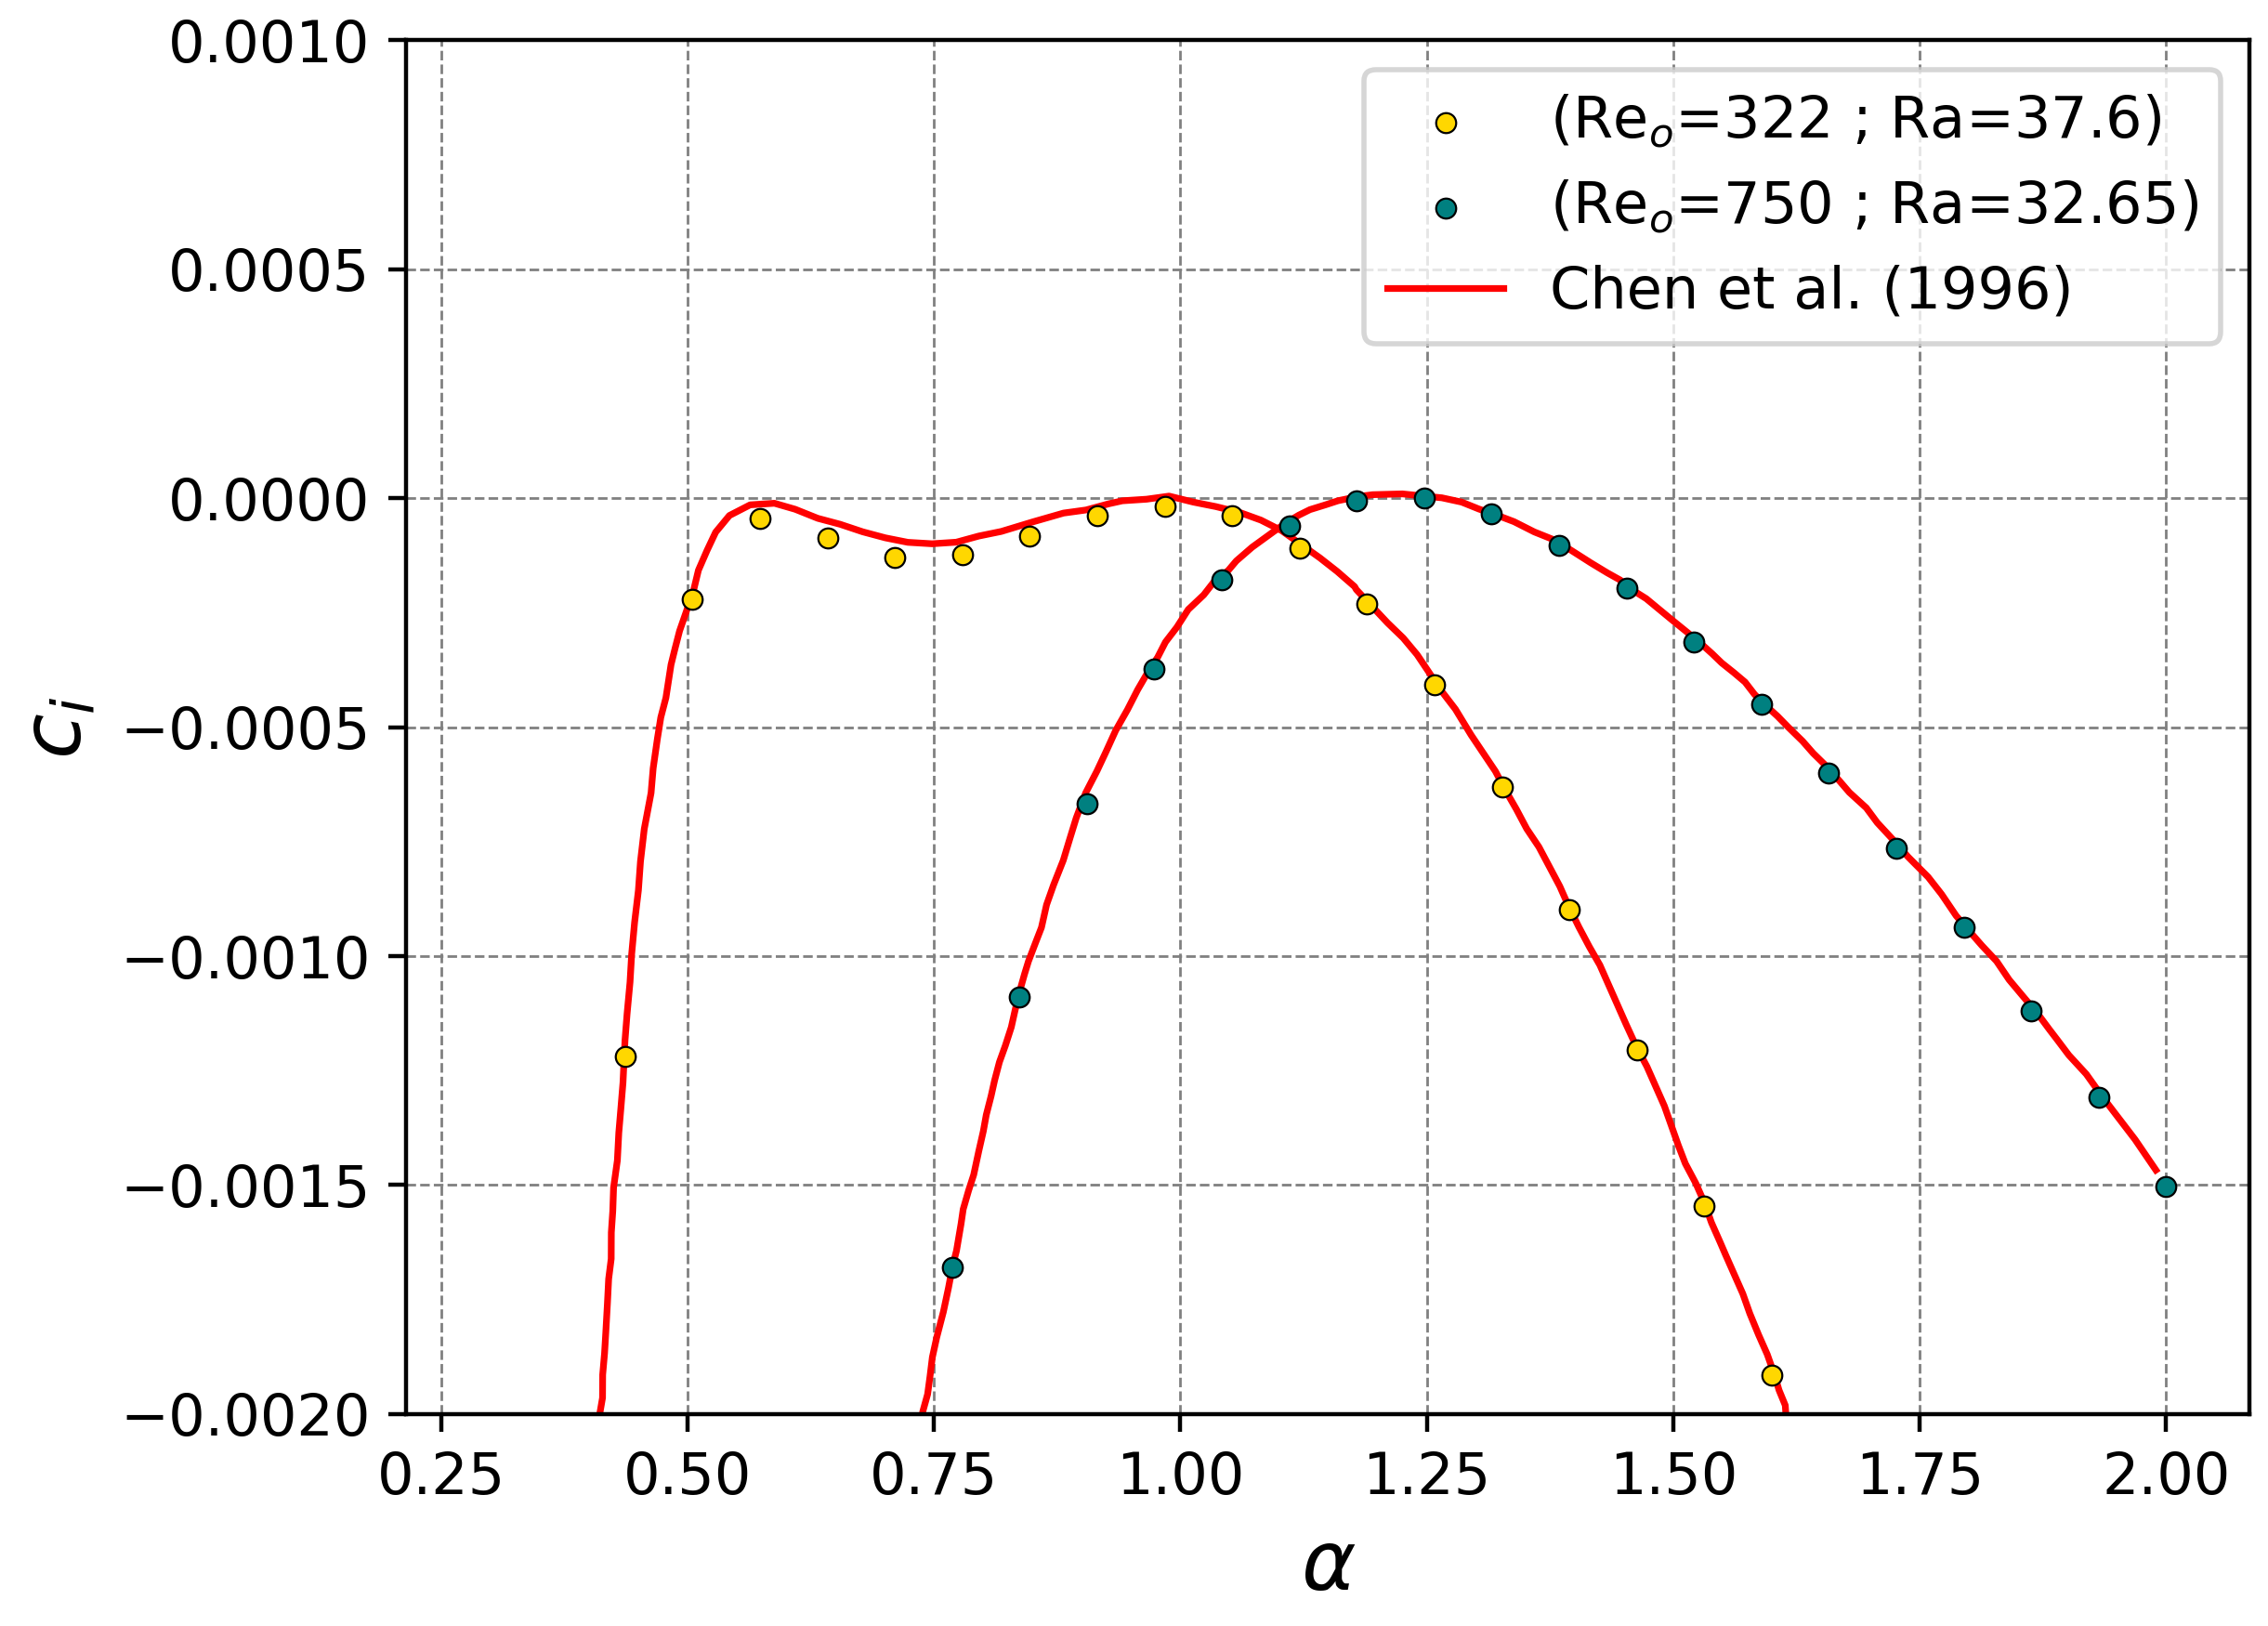
\includegraphics[width=0.6\textwidth]{figures/cap4/osmc/eigenvalues.png}
	 \caption{Variación de $c_i$ con $\alpha$ para diferentes valores de Re$_o$ con sus valores de Ra.} 
 \label{fig:eigenval_alpha}
\end{figure}


\subsection{Autofunciones}

\paragraph{Normalización.}
Sea $\{y_j\}_{j=1}^{N}$ la malla discreta en la dirección $Y$, las autofunciones \linebreak discretas $\{\widehat{v_x}(y_j),\widehat{v_y}(y_j),\widehat{v_z}(y_j),\widehat{\theta}(y_j)\}_{j=1}^{N}$ se normalizan localizando el índice donde el módulo de $\widehat{v_x}$ alcanza su valor máximo. Dicho índice se expresa de la siguiente forma:
$$
j_\star \;=\; \arg\max_{1\le j\le N}\,\big|\widehat{v_x}(y_j)\big|, 
\qquad 
\max_{1\le j\le N}\big|\widehat{v_x}(y_j)\big| \;=\; \big|\widehat{v_x}(y_{j_\star})\big|.
$$
Aquí, $\arg\max$ (argumento del máximo) denota el operador que devuelve el índice $j$ en el que la cantidad $|\widehat{v_x}(y_j)|$ alcanza su mayor valor. Luego, sea $u_\star=\widehat{v_x}(y_{j_\star})\neq 0$, se define un factor de normalización $c \in \mathbb{C}$ de forma tal que $\mathbb{R}\text{e}[c \, \widehat{v_x}(y_{j_\star})]=1$ y $\mathbb{I}\text{m}[c \, \widehat{v_x}(y_{j_\star})]=0$. A partir de estas dos condiciones se llega a que $c$ debe tener la forma:
$$
c \;:=\; \frac{\overline{u_\star}}{|u_\star|^2} \;=\; \frac{1}{u_\star}
$$
donde $\overline{(\text{.})}$ indica complejo conjugado. Con el mismo $c$ se normalizan todas las autofunciones, para todo $j$, se tiene:
$$
\boldsymbol{\widehat{v}}_{\mathrm{norm}}(y_j)=c\,\boldsymbol{\widehat{v}}(y_j) \text{ ,} \quad
\widehat{\theta}_{\mathrm{norm}}(y_j)=c\,\widehat{\theta}(y_j).
$$
Nótese que si $u_\star=0$, la normalización anterior no aplica. Esta normalización es la empleada por Zang y Krist en su trabajo \cite{zang1989numerical} y es la que se utiliza por convención en la mayoría de la bibliografía.


En la Figura \ref{fig:eigenfun_valid} se presentan las autofunciones correspondientes al autovalor más inestable asociado a los parámetros $\text{Re}_o=1125$, $\text{Ra}=2500$ y Pr = 0.7. La Figura \ref{fig:eigenfun_2d} expone la autofunción de la velocidad \textit{streamwise} y de la temperatura para el caso de una onda 2D al considerar $\alpha=1$ y $\beta=0$. Por su parte, la Figura \ref{fig:eigenfun_3d} presenta las autofunciones de las mismas magnitudes para una onda 3D ahora considerando $\alpha=1$ y $\beta=1$. Ambos casos se comparan con las autofunciones calculadas por Chen y Chung \cite{chen2003direct}. Debe aclararse que los autores emplean una normalización distinta a la definida más arriba: cada una de las autofunciones $\left\lbrace \widehat{v_x}(y), \widehat{v_y}(y), \widehat{v_z}(y), \widehat{\theta}(y) \right\rbrace$ se normalizan por separado\footnote{Es decir, para cada autofunción considerada, se calcula una constante compleja $c$ diferente.} de modo que el máximo de la parte real sea igual a uno y su parte imaginaria sea nula. Al considerar esto y comparar las autofunciones obtenidas a partir de OSMC, con aquellos obtenidos por Chen y Chung, es posible apreciar un excelente acuerdo.

\newpage

\begin{figure}[H]
 \centering
  \subfloat[]{
    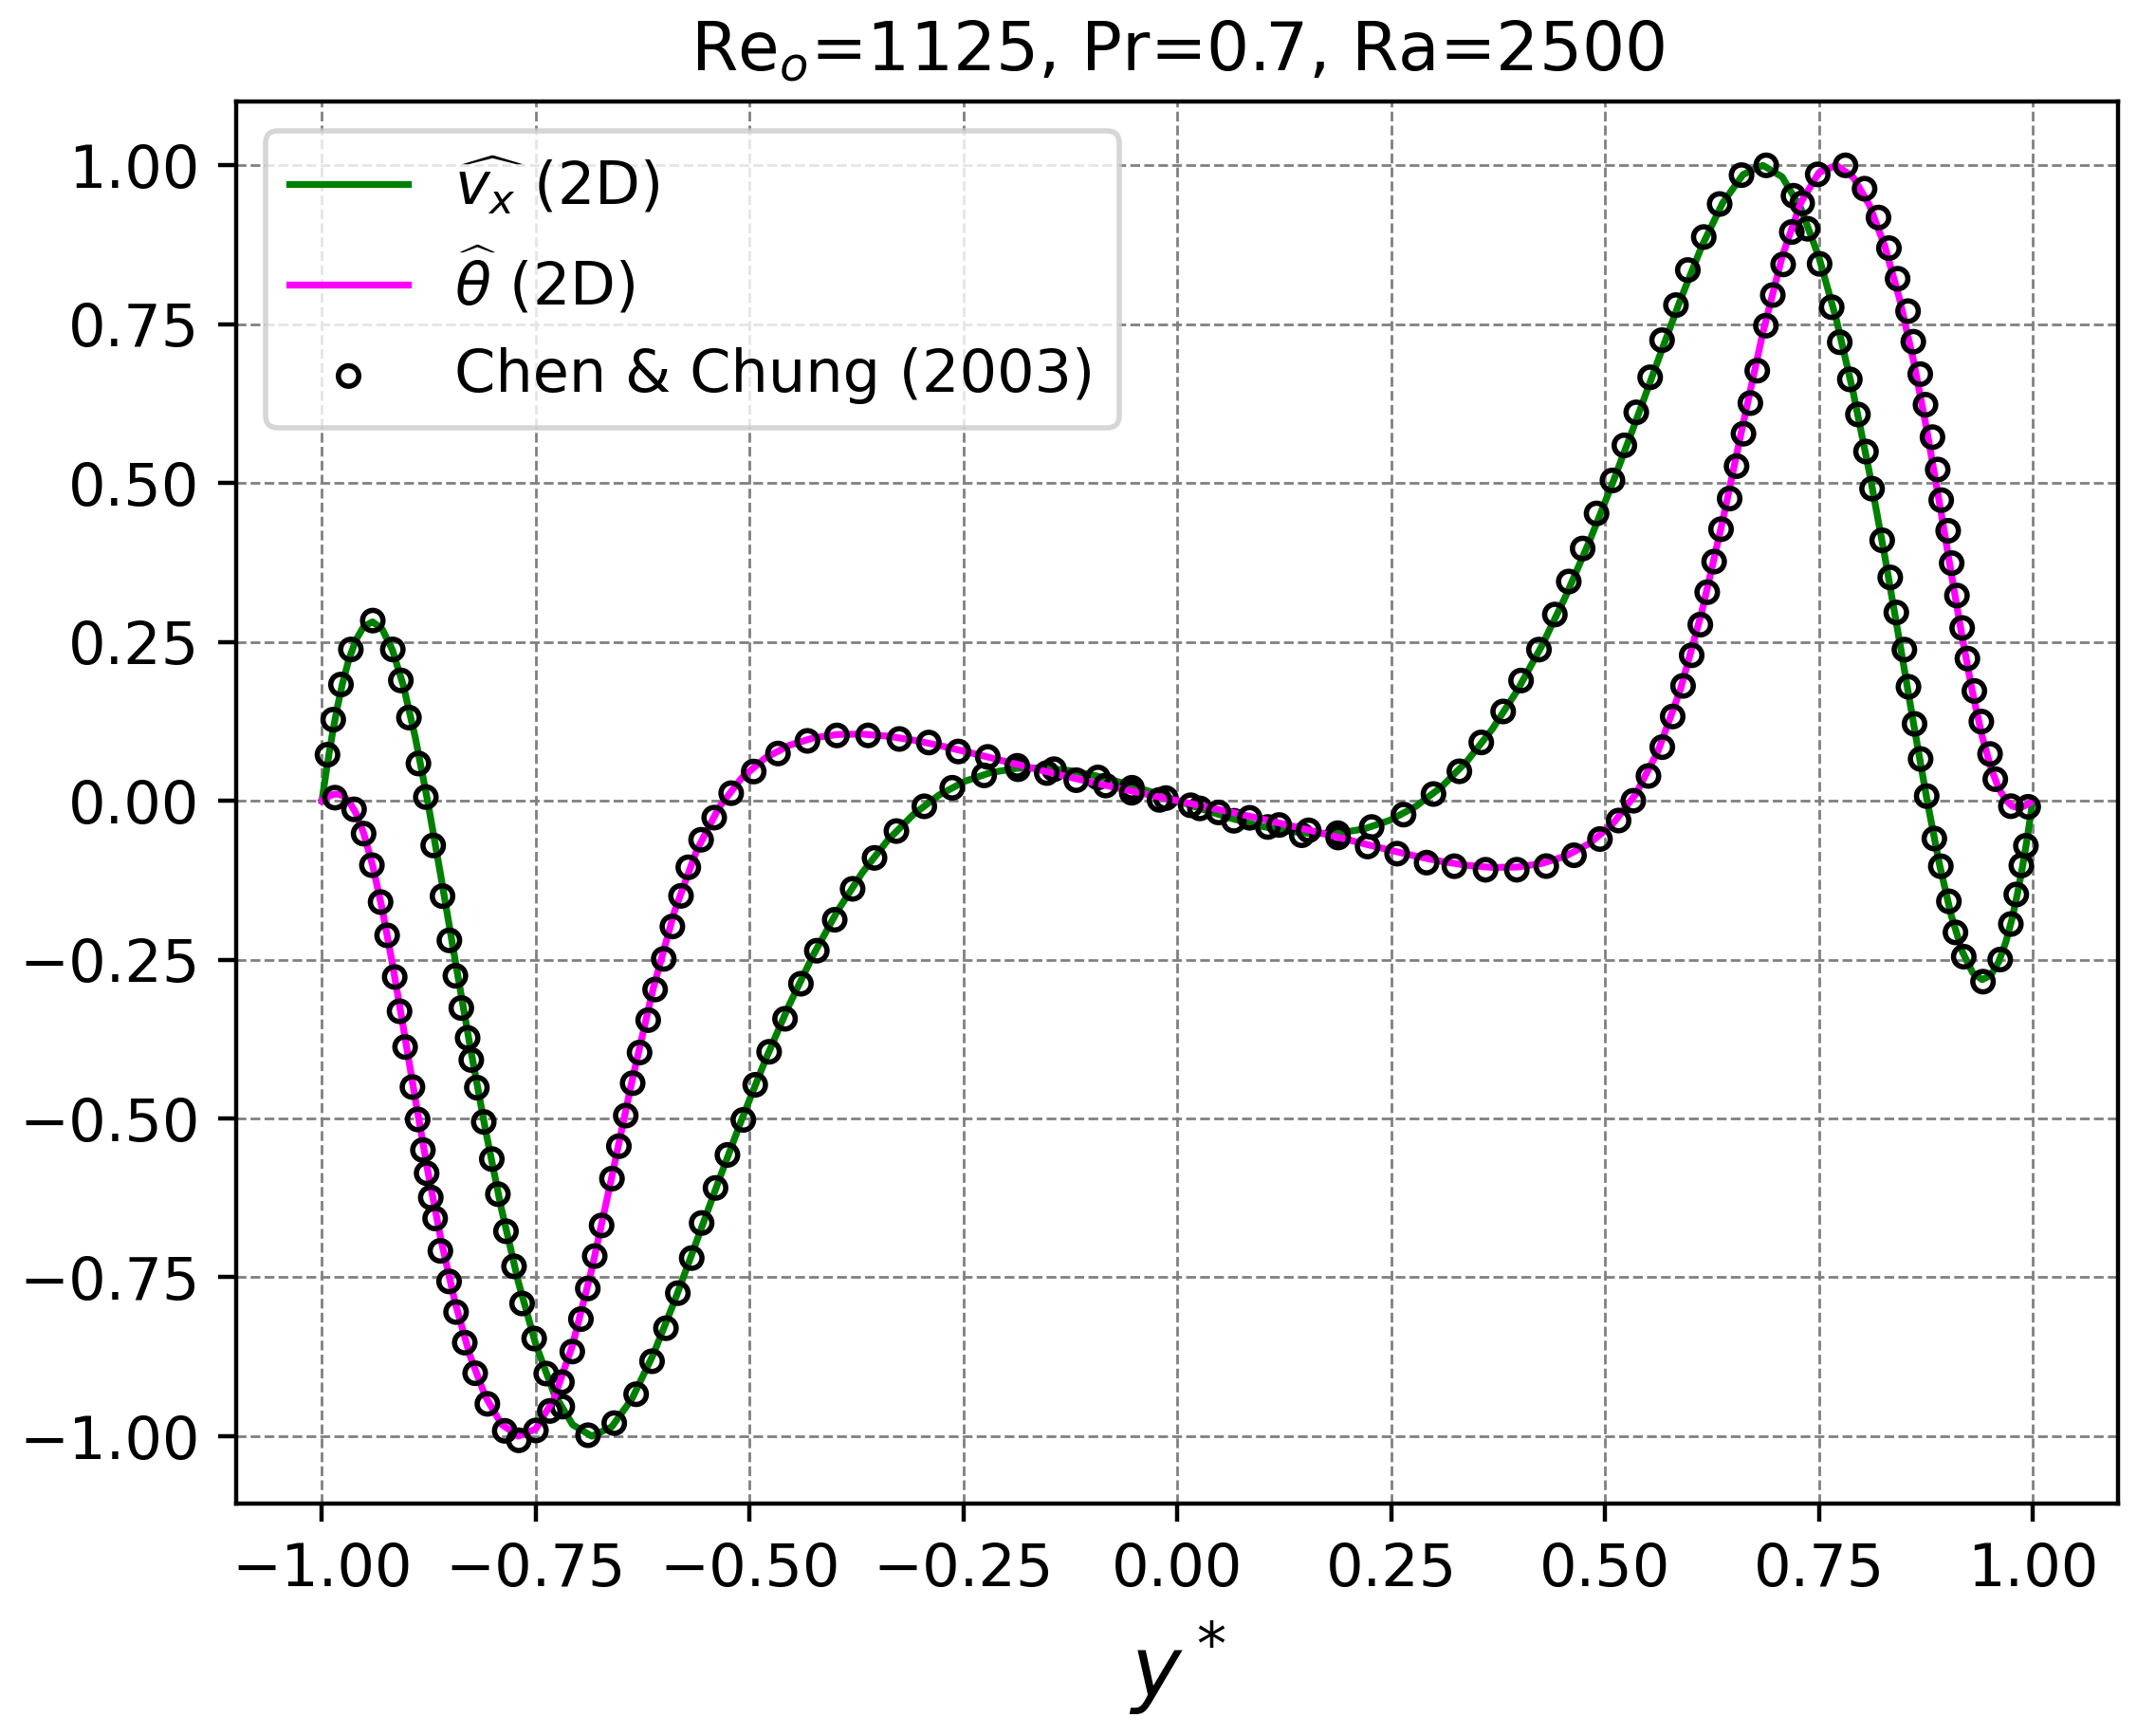
\includegraphics[width=0.49\textwidth]{figures/cap4/osmc/validation_eigenfuncs_2d.png}
    	\label{fig:eigenfun_2d}}  
    \subfloat[]{
    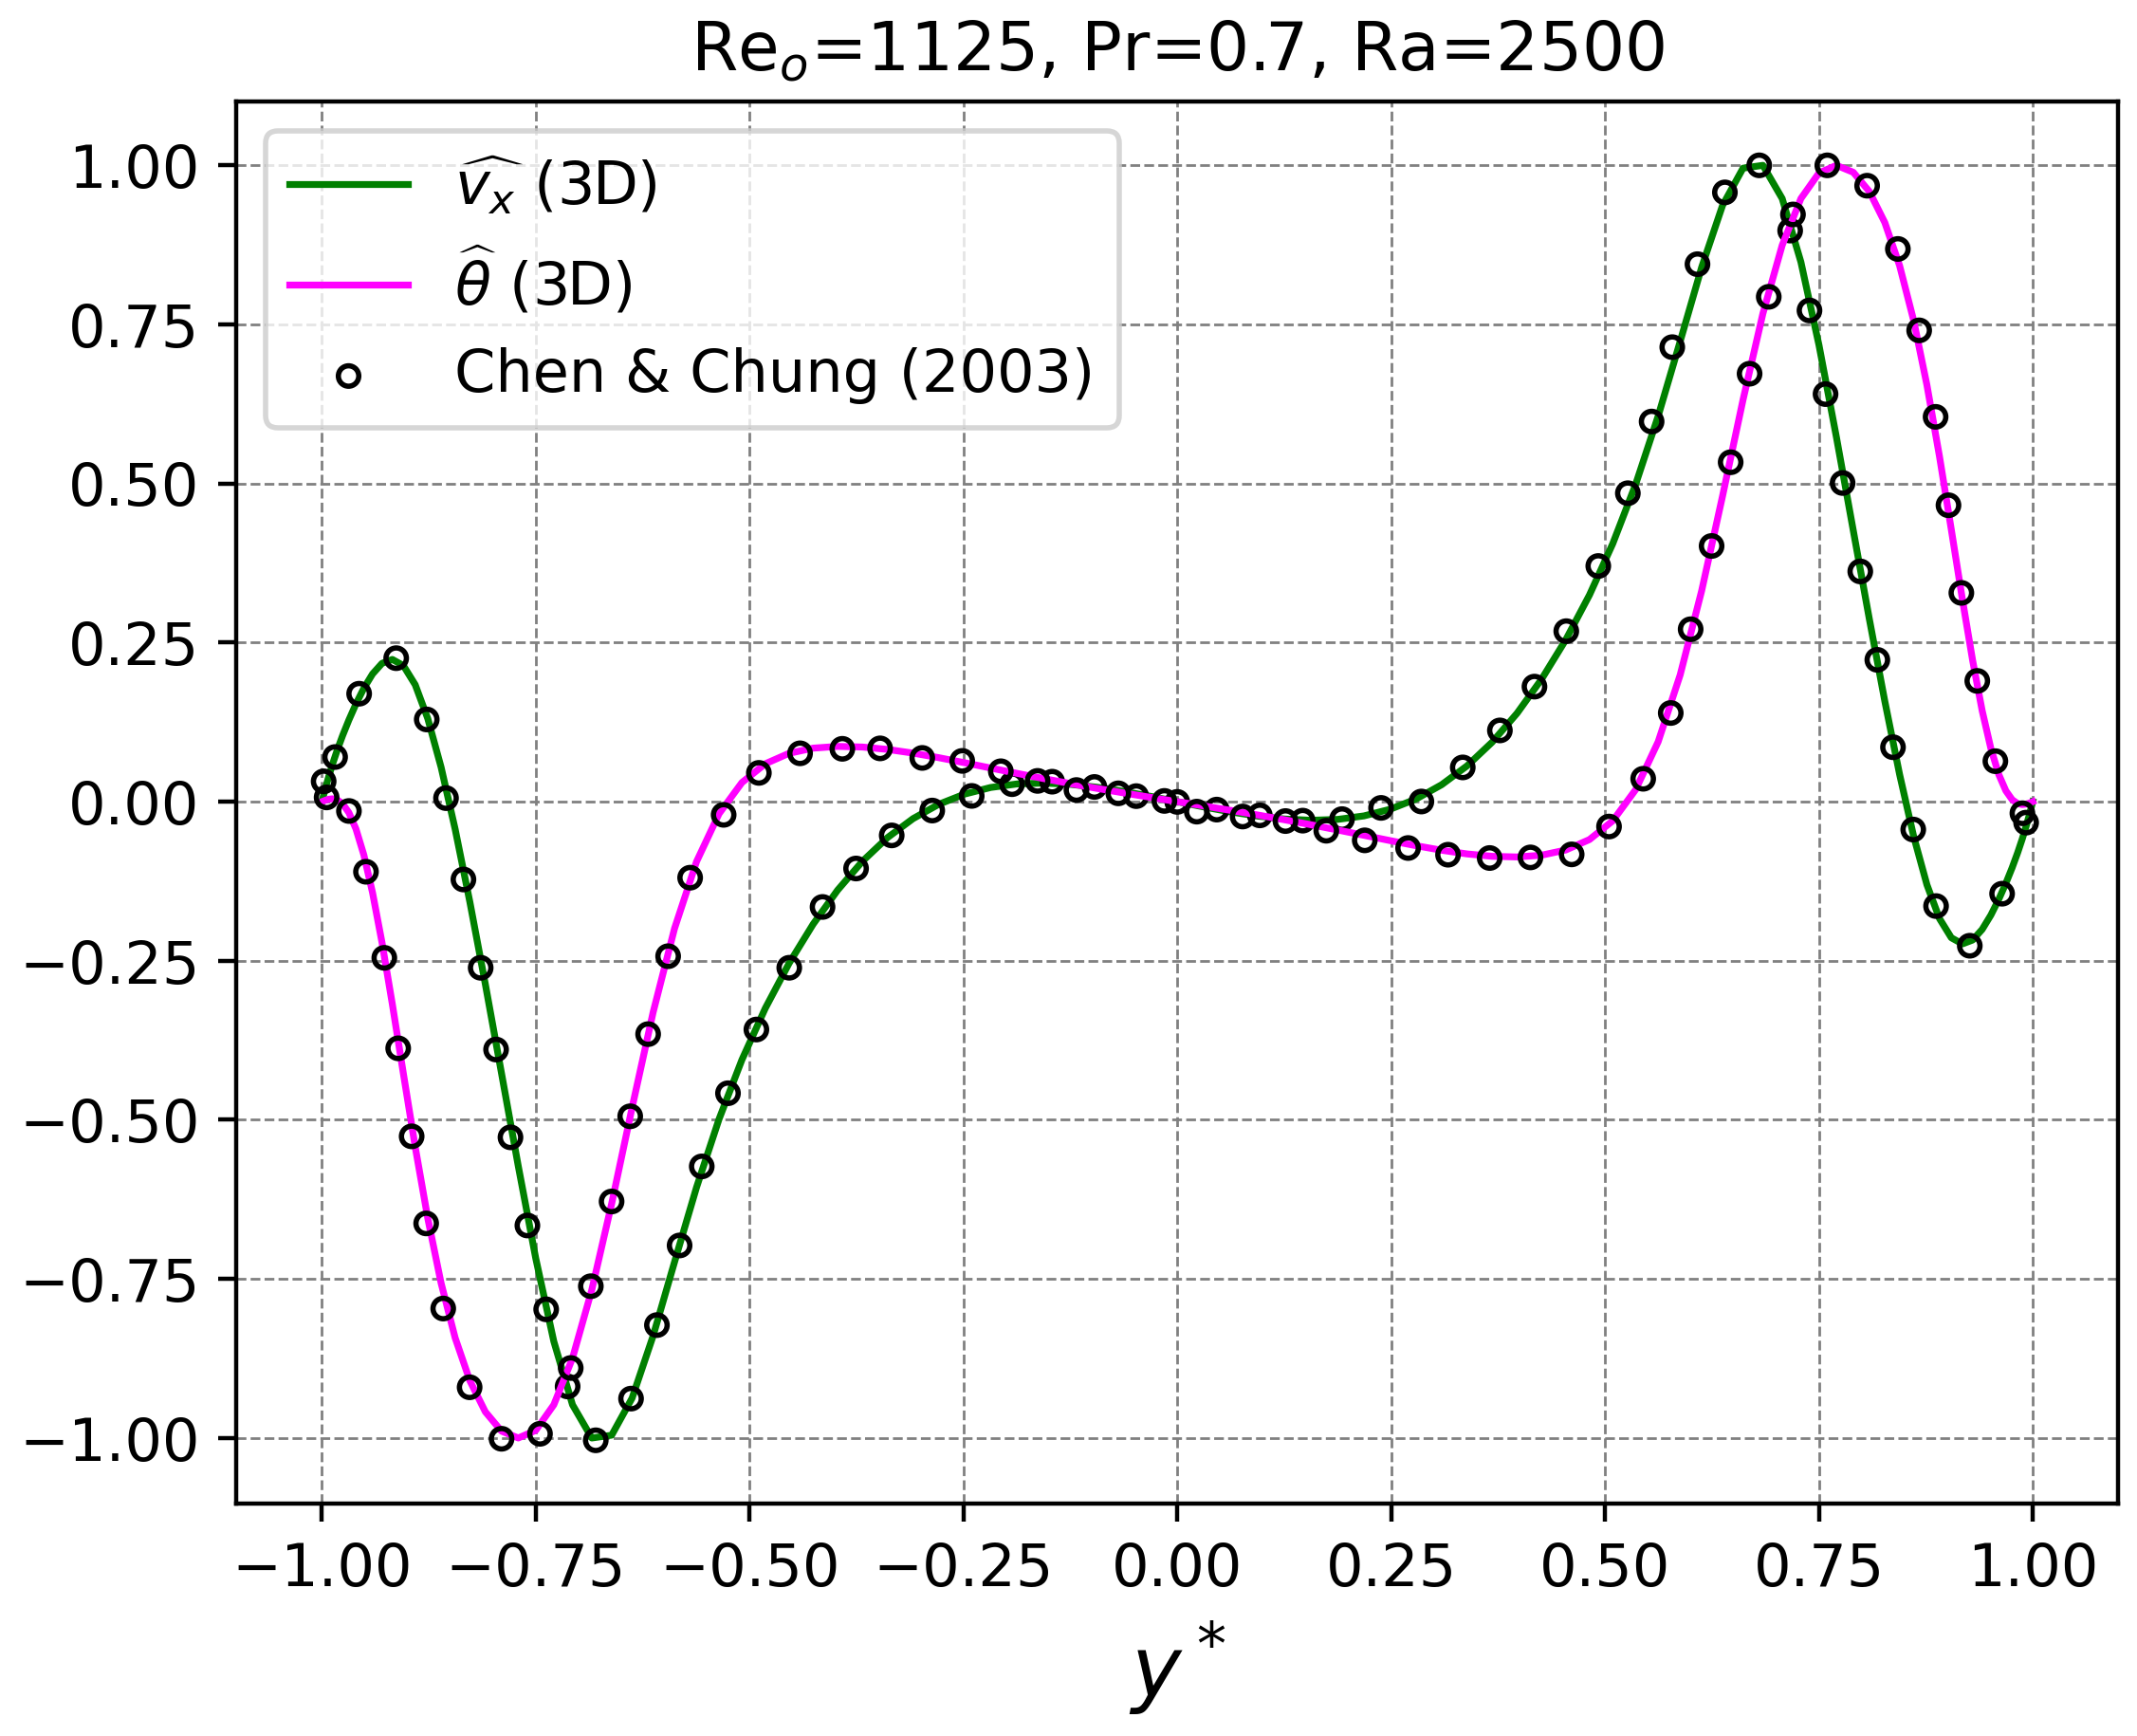
\includegraphics[width=0.49\textwidth]{figures/cap4/osmc/validation_eigenfuncs_3d.png}
    	\label{fig:eigenfun_3d}}  
 	\caption{Parte real de las autofunciones asociadas al modo más inestable para $\text{Re}_o=1125$, $\text{Ra}=2500$ y Pr = 0.7; \textbf{(a)} Onda 2D con ($\alpha$,$\beta$) = (1,0) y \textbf{(b)} Onda 3D con ($\alpha$,$\beta$) = (1,1).} 
 \label{fig:eigenfun_valid}
\end{figure}

\section{Análisis de Estabilidad Lineal versus DNS}

Como se menciona en la Sección \ref{line_an}, el análisis de estabilidad lineal predice a través de un modelo matemático la evolución temporal de pequeñas perturbaciones que son impuestas al flujo base. En esta sección, se realizan simulaciones DNS para un canal de placas paralelas, con flujo de calor constante en las paredes, cuya condición inicial se construye utilizando el autovalor más inestable y su autofunción asociada. En ese sentido, se pretende comparar las predicciones teóricas con los resultados arrojados por simulaciones realizadas con XC3D. Esto se realiza en escalas de tiempo donde las perturbaciones se mantienen relativamente acotadas (lo que hace válida a la aproximación del modelo lineal). Las condiciones iniciales de la simulación se construyen como la suma del flujo laminar, ecuaciones \ref{eq:vel_asist_boyant} - \ref{eq:theta_opo_boyant}, y las perturbaciones \ref{eq:init_con_1} - \ref{eq:init_con_3}. 

Se comparan dos casos, denominados\footnote{Nótese que Rama Izquiera y Rama Derecha hacen referencia a las ``ramas'' o ``brazos'' del espectro de autovalores considerado (véase Figura \ref{fig:Ra65RD-2d} y/o \ref{fig:Ra65RI-2d}).} Rama Izquierda (RI) y Rama Derecha (RD), que corresponden a casos físicos donde se incrementa y se disminuye la amplitud de la perturbación inicial, respectivamente. Esto, matemáticamente, equivale a una parte imaginaria negativa (RI) y positiva (RD). Los números adimensionales empleados corresponden a $\text{Re}_o=750$, $\text{Pr}=0\text{.}7$ y $\text{Ra}=65$. Los parámetros de simulación de ambos casos se exponen en la \linebreak Tabla \ref{tab:caseslineal-theor}. Obsérvese que se utilizan perturbaciones compuestas únicamente de ondas bidimensionales. Las Figuras \ref{fig:Ra65RD-2d} (RD) y \ref{fig:Ra65RI-2d} (RI) muestran, de izquierda a derecha: (i) el espectro de autovalores (puntos celestes) con el autovalor seleccionado (punto rojo); (ii) las autofunciones de las componentes de la velocidad; y (iii) la autofunción de la temperatura. Las simulaciones DNS realizadas se corren un total de 20 unidades temporales.

\begin{table}[H]
\centering
\resizebox{\textwidth}{!}{%
\begin{tabular}{lccccccccc}
\toprule
Caso & L$_x \times$ L$_y \times$ L$_z$ & N$_x \times$ N$_y \times$ N$_z$ & $\Delta t^*$ & $\alpha$ & $\beta$ & A$_{2D}$ & A$_{3D}$ & $c_{2D}$ \\
\midrule
RI & $2 \pi / \alpha \times 2 \times 2 \pi $ & $160 \times 161 \times 160$ & 0.001 & 1.22 & 0 & 0.2 \% & 0 \% & 0.656 - 0.0237 j \\
RD & $2 \pi / \alpha \times 2 \times 2 \pi $ & $160 \times 161 \times 160$ & 0.001 & 1.22 & 0 & 0.2 \% & 0 \% & 1.239 + 0.042 j \\
\bottomrule
\end{tabular}}
\caption{Parámetros de simulación de los dos casos elegidos.}
\label{tab:caseslineal-theor}
\end{table}

\begin{figure}[H]
 \centering 
  \subfloat[]{
    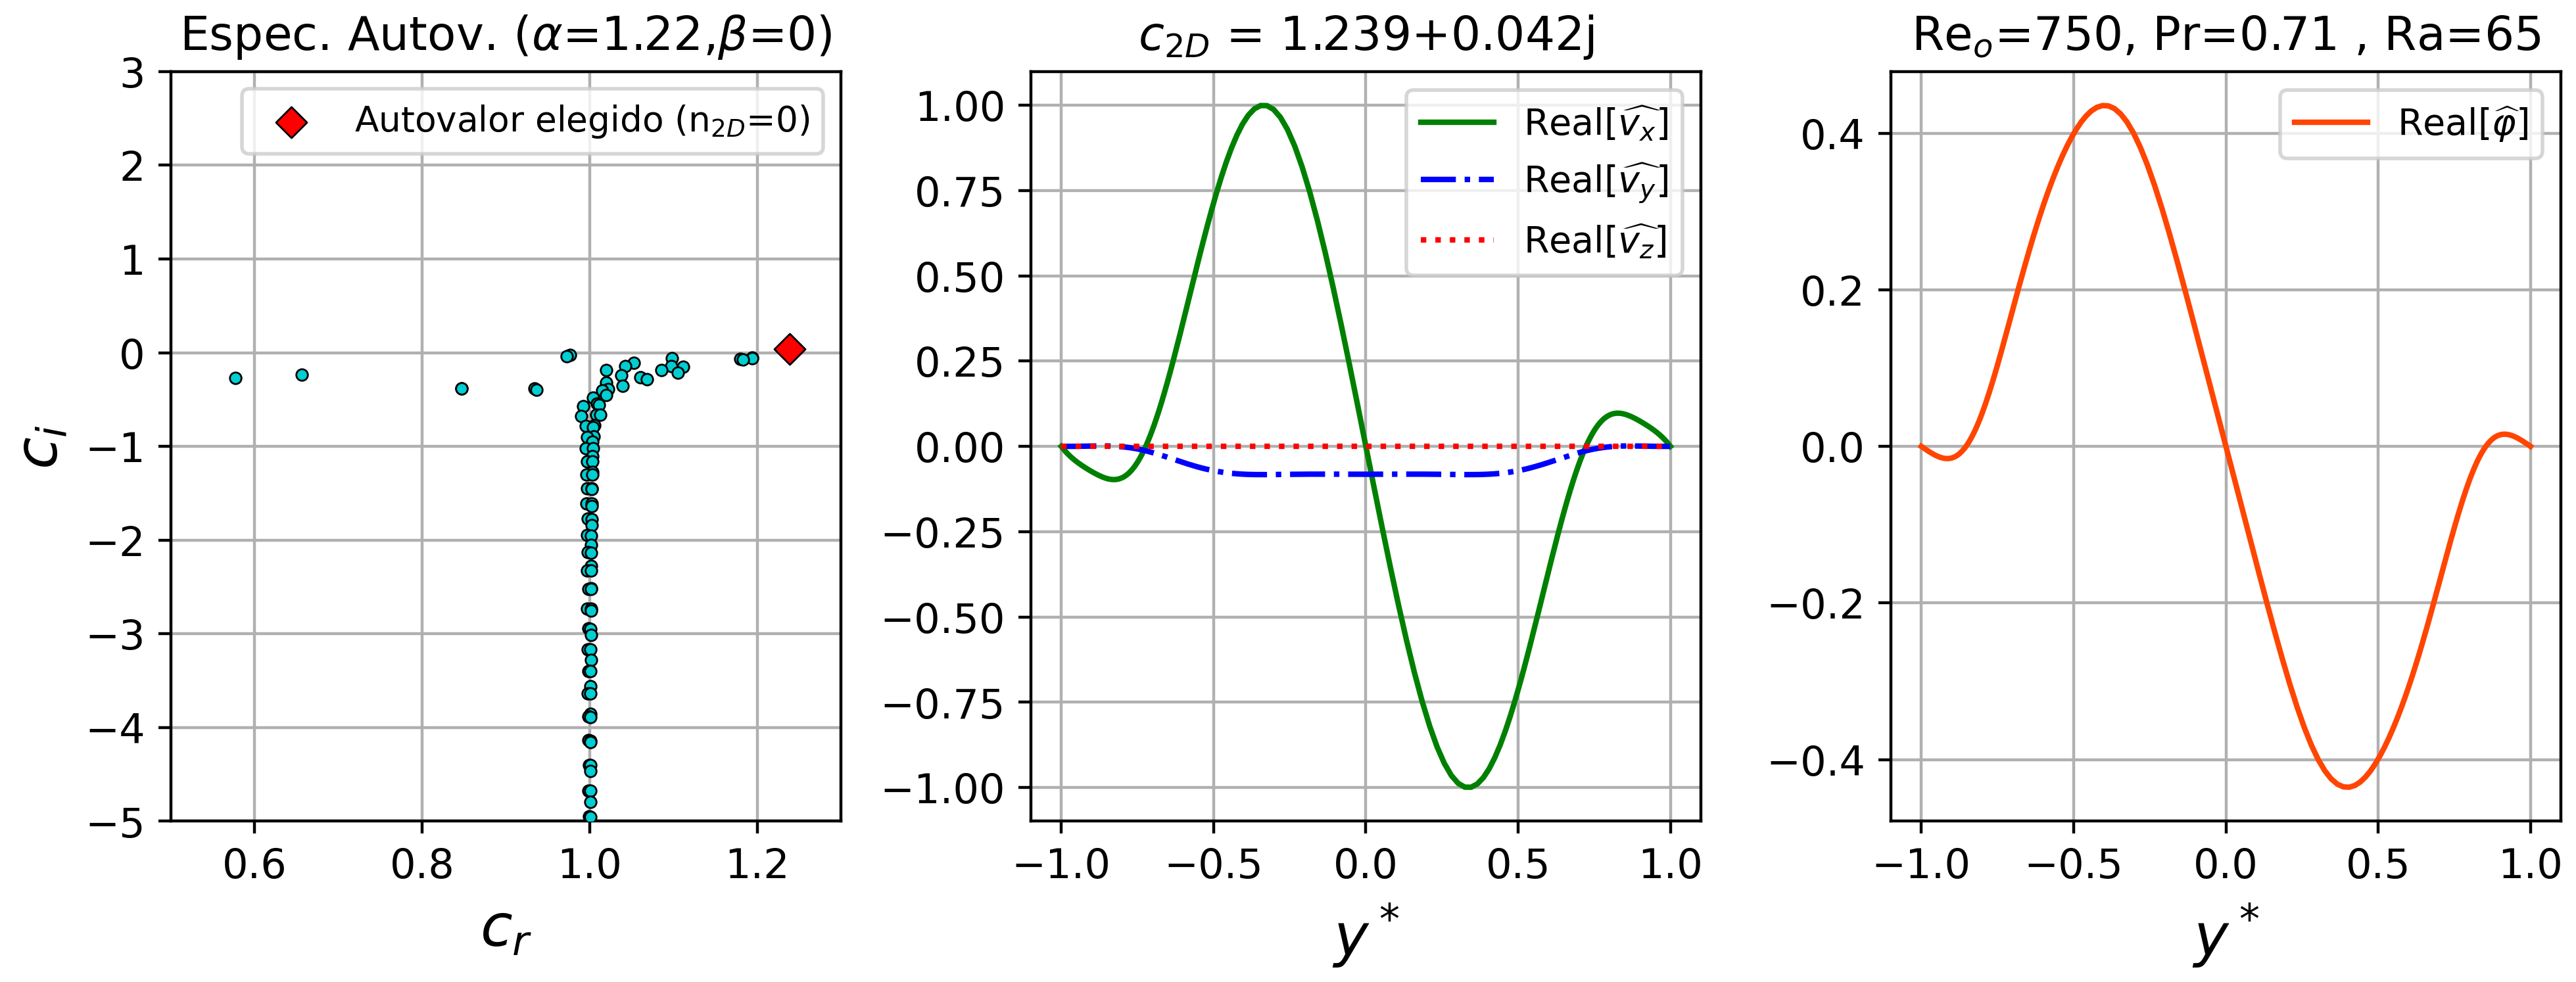
\includegraphics[width=0.8\textwidth]{figures/cap4/osmc/Ra65_RamaDer/2d_eigenfun.png}
    \label{fig:Ra65RD-2d}}
      
    \subfloat[]{
    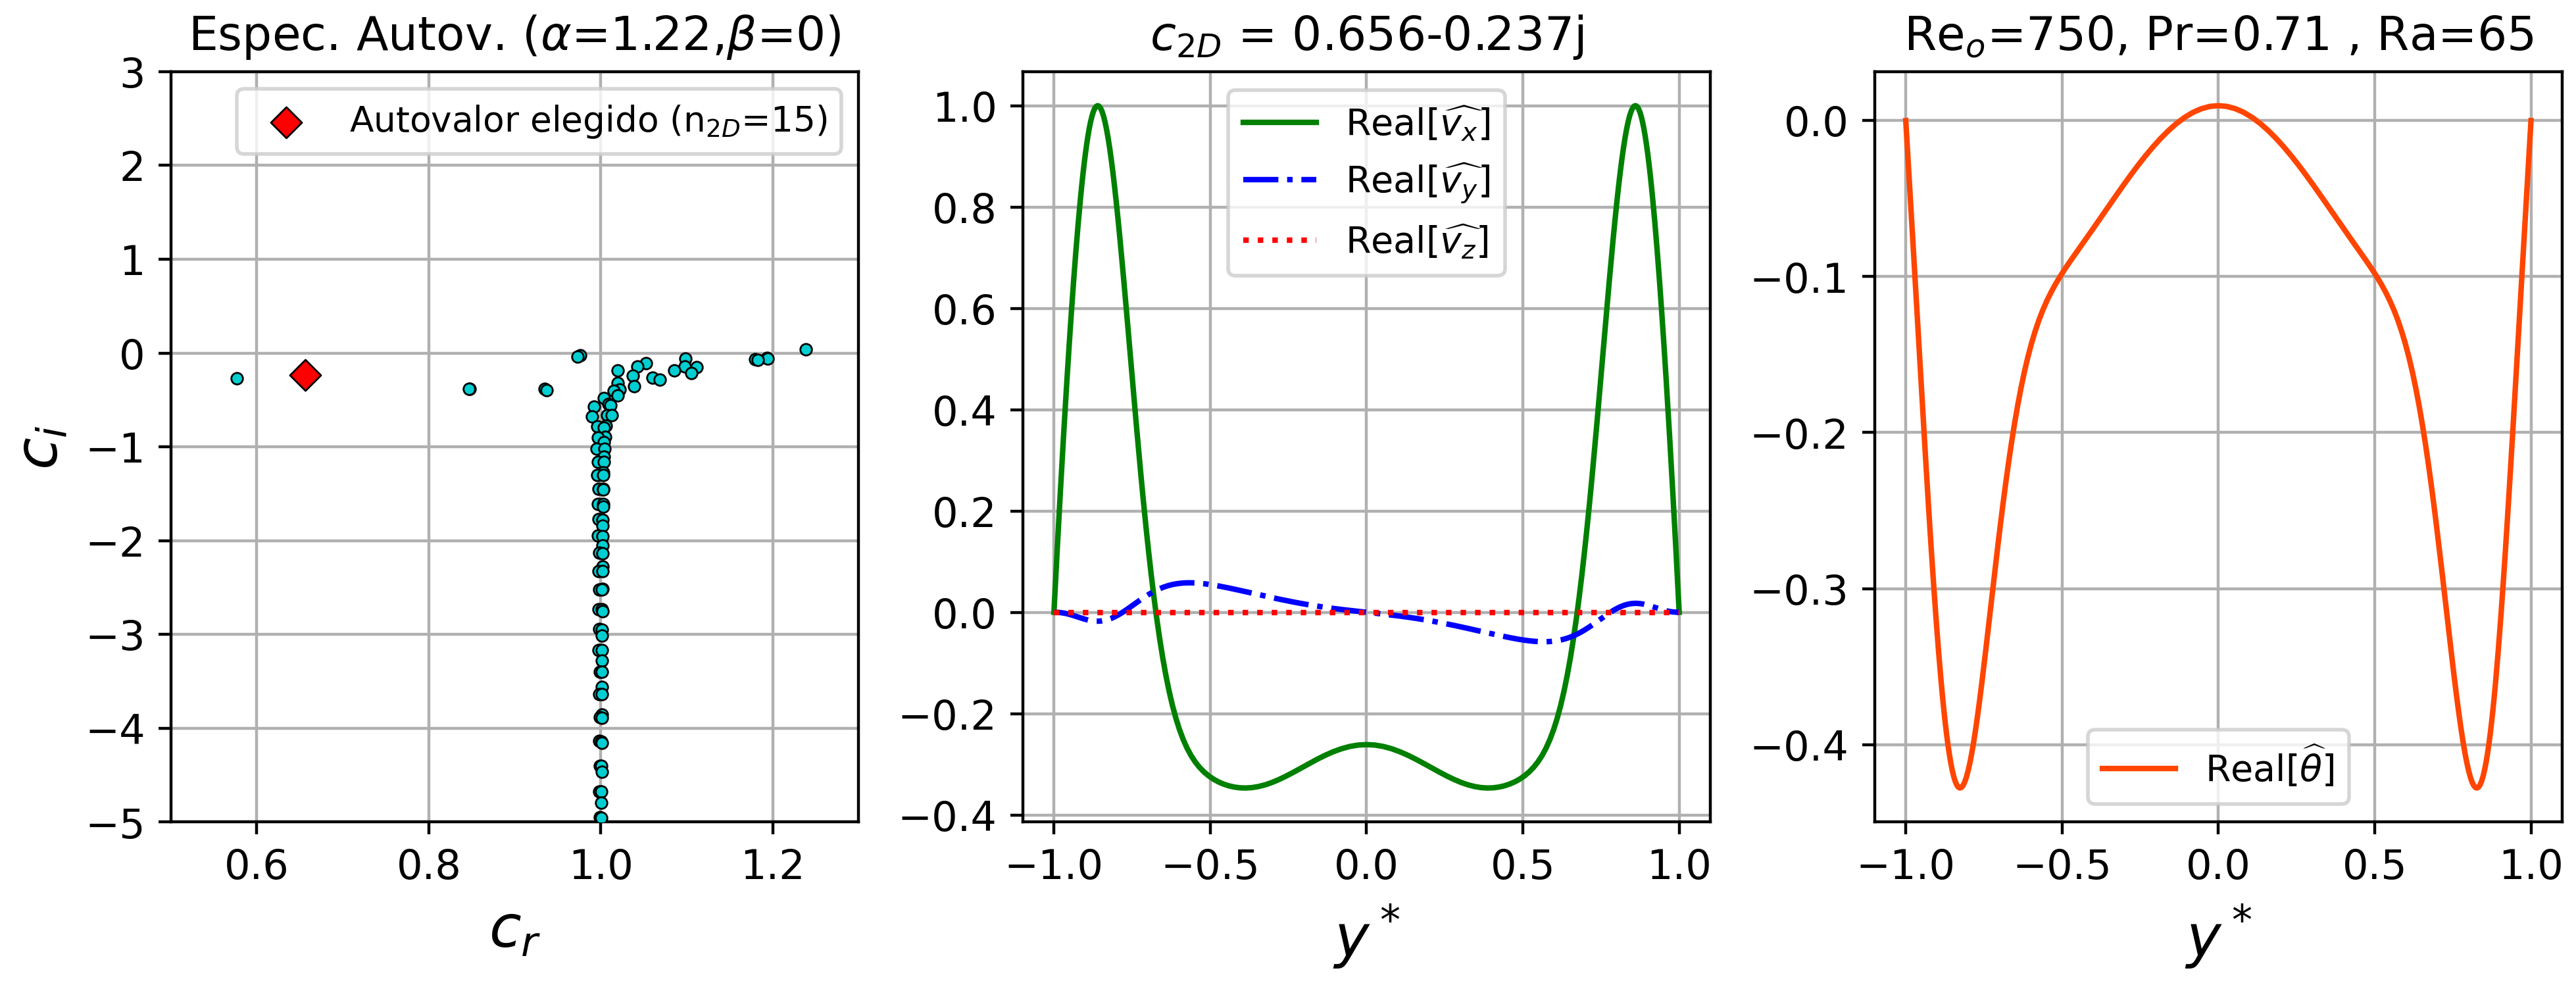
\includegraphics[width=0.8\textwidth]{figures/cap4/osmc/Ra65_RamaIzq/2d_eigenfun.png}
    \label{fig:Ra65RI-2d}}  
 \caption{De izquierda a derecha: (i) espectro de autovalores (puntos celestes) con el autovalor seleccionado (punto rojo); (ii) autofunciones de las componentes de la velocidad; (iii) autofunción asociada a la temperatura. \textbf{(a)} Caso RD y \textbf{(b)} Caso RI.} 
 \label{fig:Ra65-2d}
\end{figure}



Para comprobar la predicción de la teoría de estabilidad lineal con aquella producida por las herramientas numéricas, se emplea la evolución temporal de la energía cinética turbulenta (TKE) y de la varianza de la temperatura. En XC3D, dichas magnitudes corresponden al promedio integral en $y^*$ de las correlaciones $( \langle u^{* \prime}_x u^{* \prime}_x \rangle + \langle u^{* \prime}_y u^{* \prime}_y  \rangle + \langle u^{* \prime}_z u^{* \prime}_z  \rangle) / 2$ y $\langle \theta^{* \prime} \theta^{* \prime} \rangle$. En teoría de estabilidad lineal dichas cantidades se aproximan utilizando las autofunciones $\left\lbrace \widehat{v_x}, \widehat{v_y}, \widehat{v_z}, \widehat{\theta} \right\rbrace$ y las expresiones tipo \ref{eq:waves3d} para obtener:
\begin{align}
\text{TKE} &= \frac{1}{2} (A_{2D})^2 \hspace*{0.5mm} e^{2 \alpha c_i t^*} \int \left[  ( \widehat{v_x}, \widehat{v_y}, \widehat{v_z} ) \cdot ( \widehat{v_x}, \widehat{v_y}, \widehat{v_z} )  \right] dy^* \text{ ,} \\
\int \langle \theta^{* \prime} \theta^{* \prime} \rangle dy^* &= \frac{1}{2} (A_{2D})^2 \hspace*{0.5mm} e^{2 \alpha c_i t^*} \int (\widehat{\theta})^2 dy^* \text{ .}
\end{align}   
En estas expresiones, si $c_i < 0$, las cantidades decaen y el flujo es estable. Por el contrario, si $c_i > 0$, las mismas crecen y el flujo base evoluciona en el tiempo, dando posiblemente, origen a la transición. Las afirmaciones anteriores son ciertas siempre que $\alpha$ sea positivo.

Las Figuras \ref{fig:Ra65RD-tke} y \ref{fig:Ra65RD-tvar} muestran la evolución temporal de la TKE y de la varianza de la temperatura para el caso RD. Se observa un muy buen acuerdo entre la predicción teórica y los resultados obtenidos a partir de simulaciones DNS con las herramientas numéricas utilizadas. En este caso se aprecia que la perturbación introducida logra inestabilizar el flujo (pues $c_i>0$) y que si bien en una etapa temprana el acuerdo entre ambas metodologías coincide, si el flujo transiciona a un régimen turbulento, la consistencia entre ambos debería tender a desaparecer.  

De forma completamente análoga, las Figuras \ref{fig:Ra65RI-tke} y \ref{fig:Ra65RI-tvar} muestran la evolución temporal de la TKE y de la varianza de la temperatura para el caso RI. En este caso, dado que $c_i<0$, el análisis de estabilidad lineal predice que la perturbación impuesta tenderá a decaer y el flujo no se inestabilizará. Esta predicción está en completa consistencia con la simulación DNS realizada. Esto nos permite confirmar que la implementación de la condición inicial perturbada en XC3D es correcta.  

\begin{figure}[H]
 \centering
  \subfloat[]{
    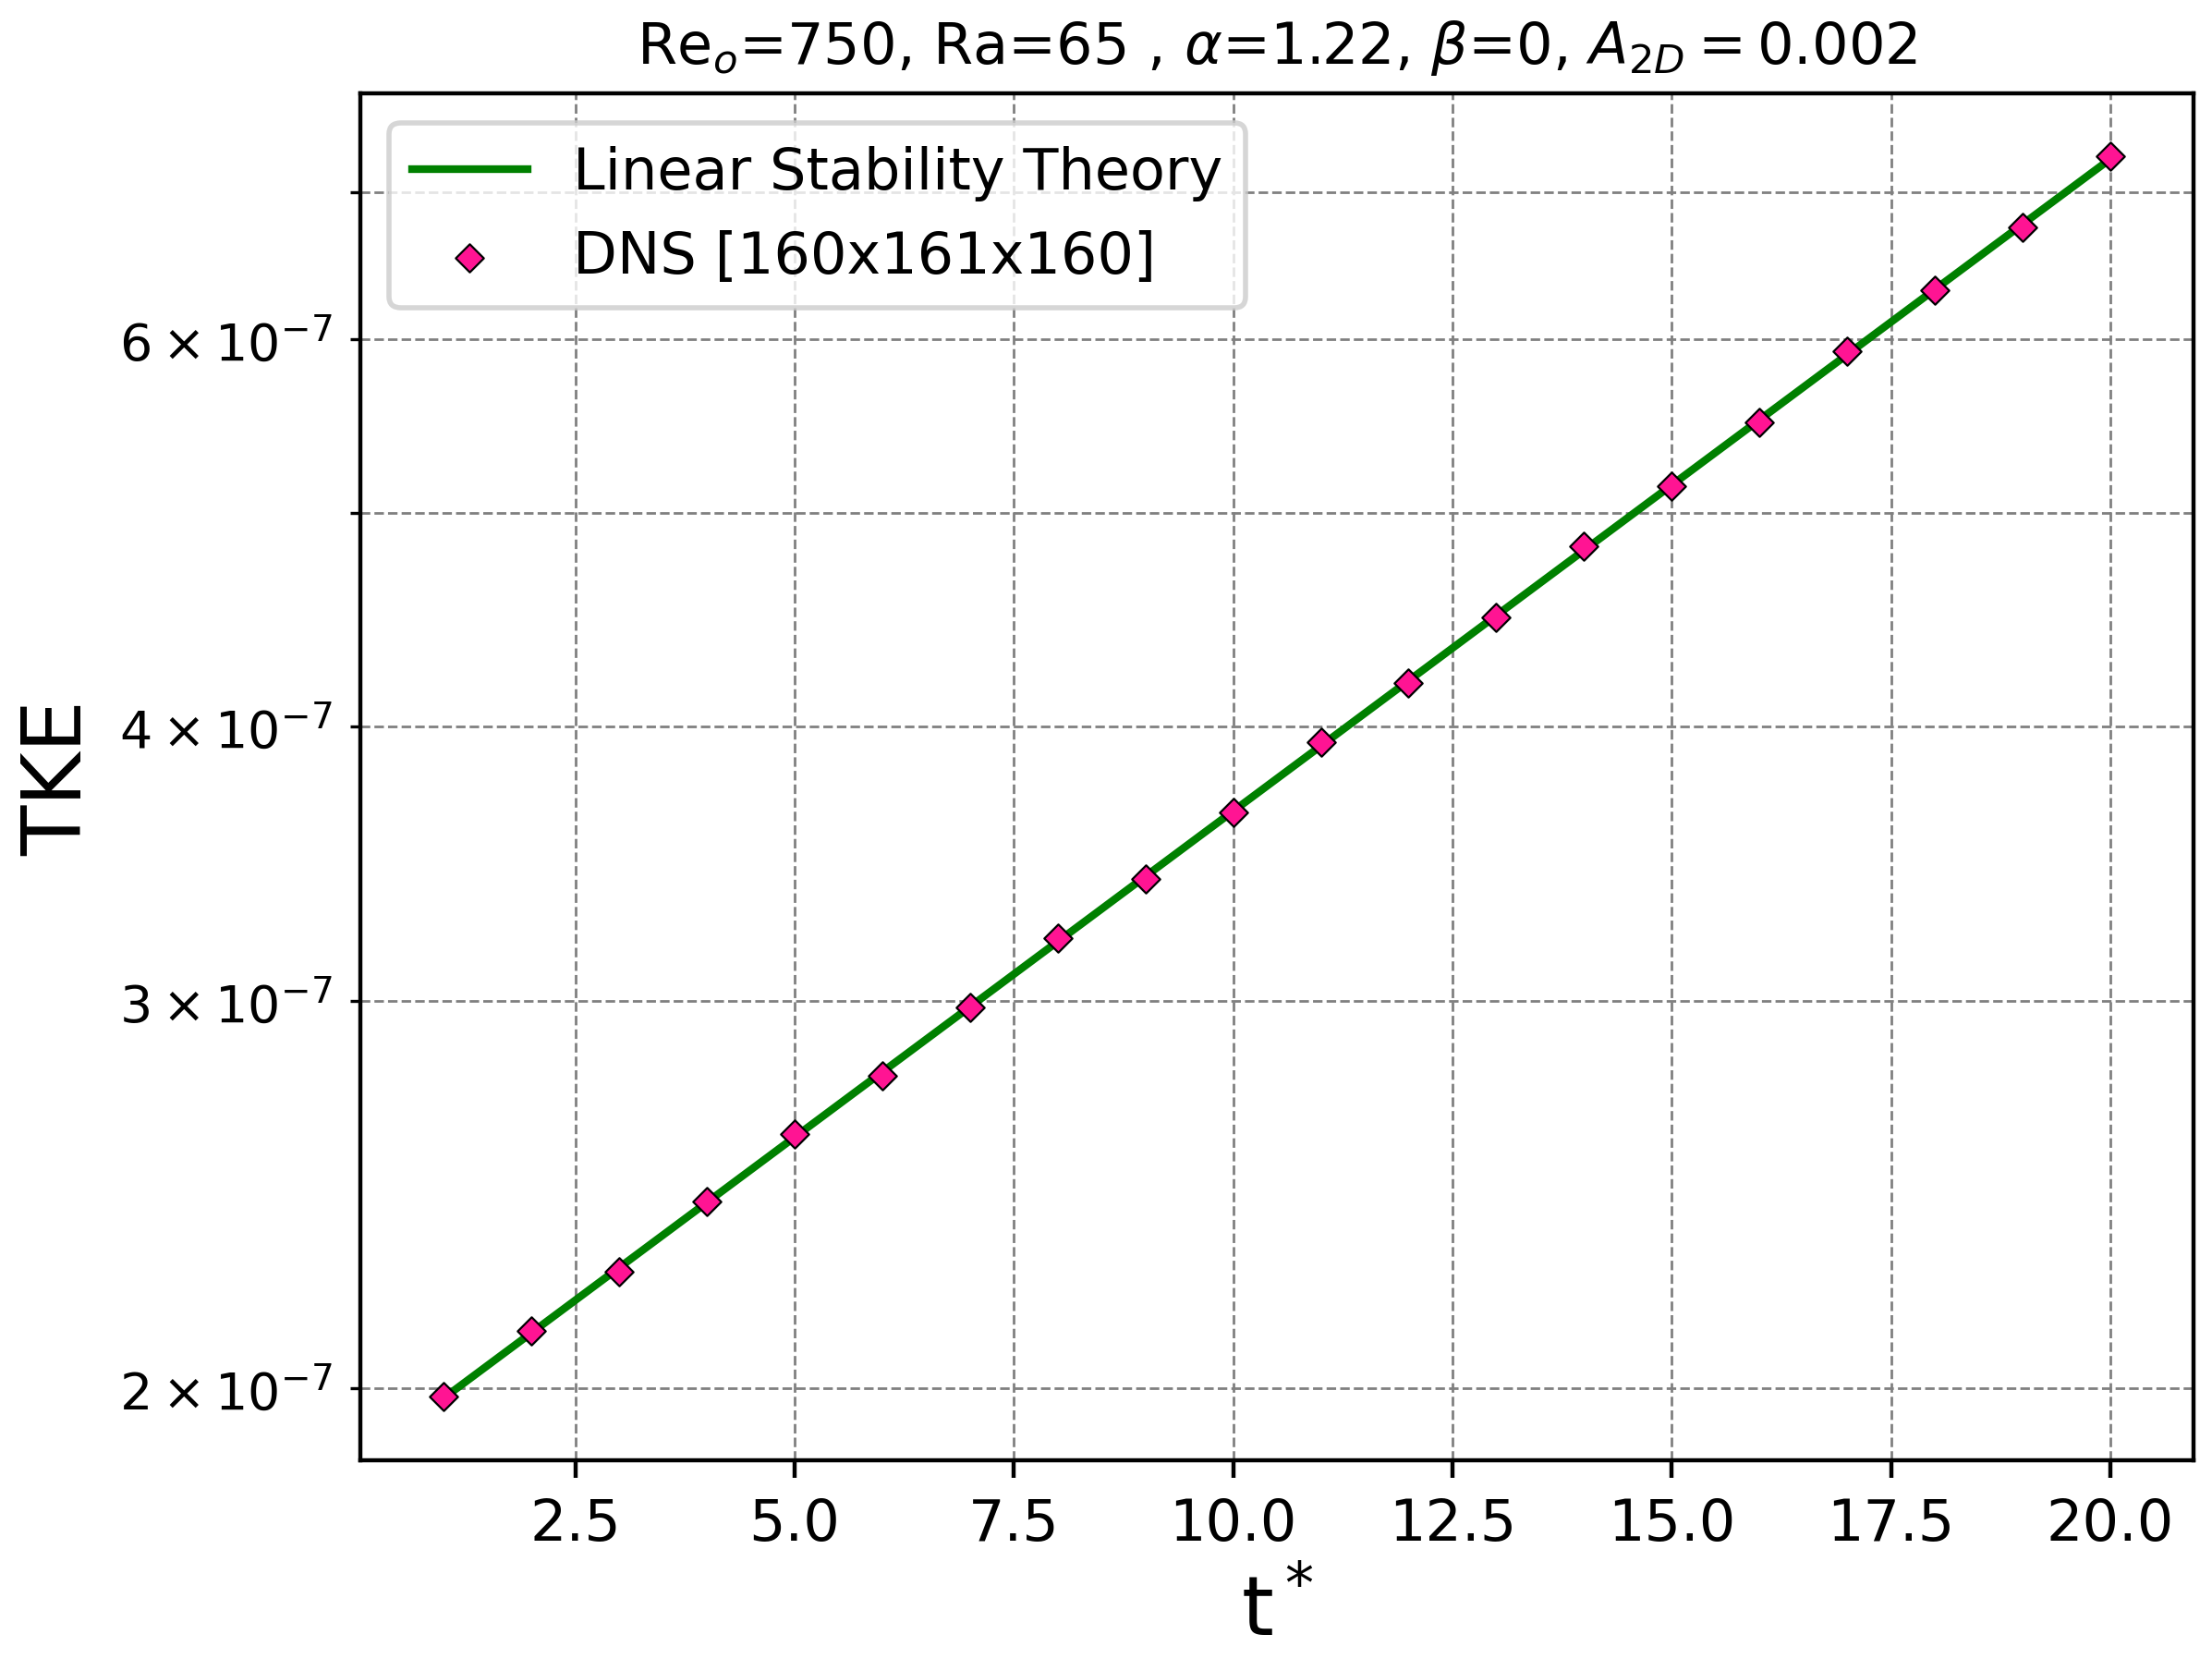
\includegraphics[width=0.49\textwidth]{figures/cap4/osmc/Ra65_RamaDer/tke.png}
    	\label{fig:Ra65RD-tke}}  
  \subfloat[]{
    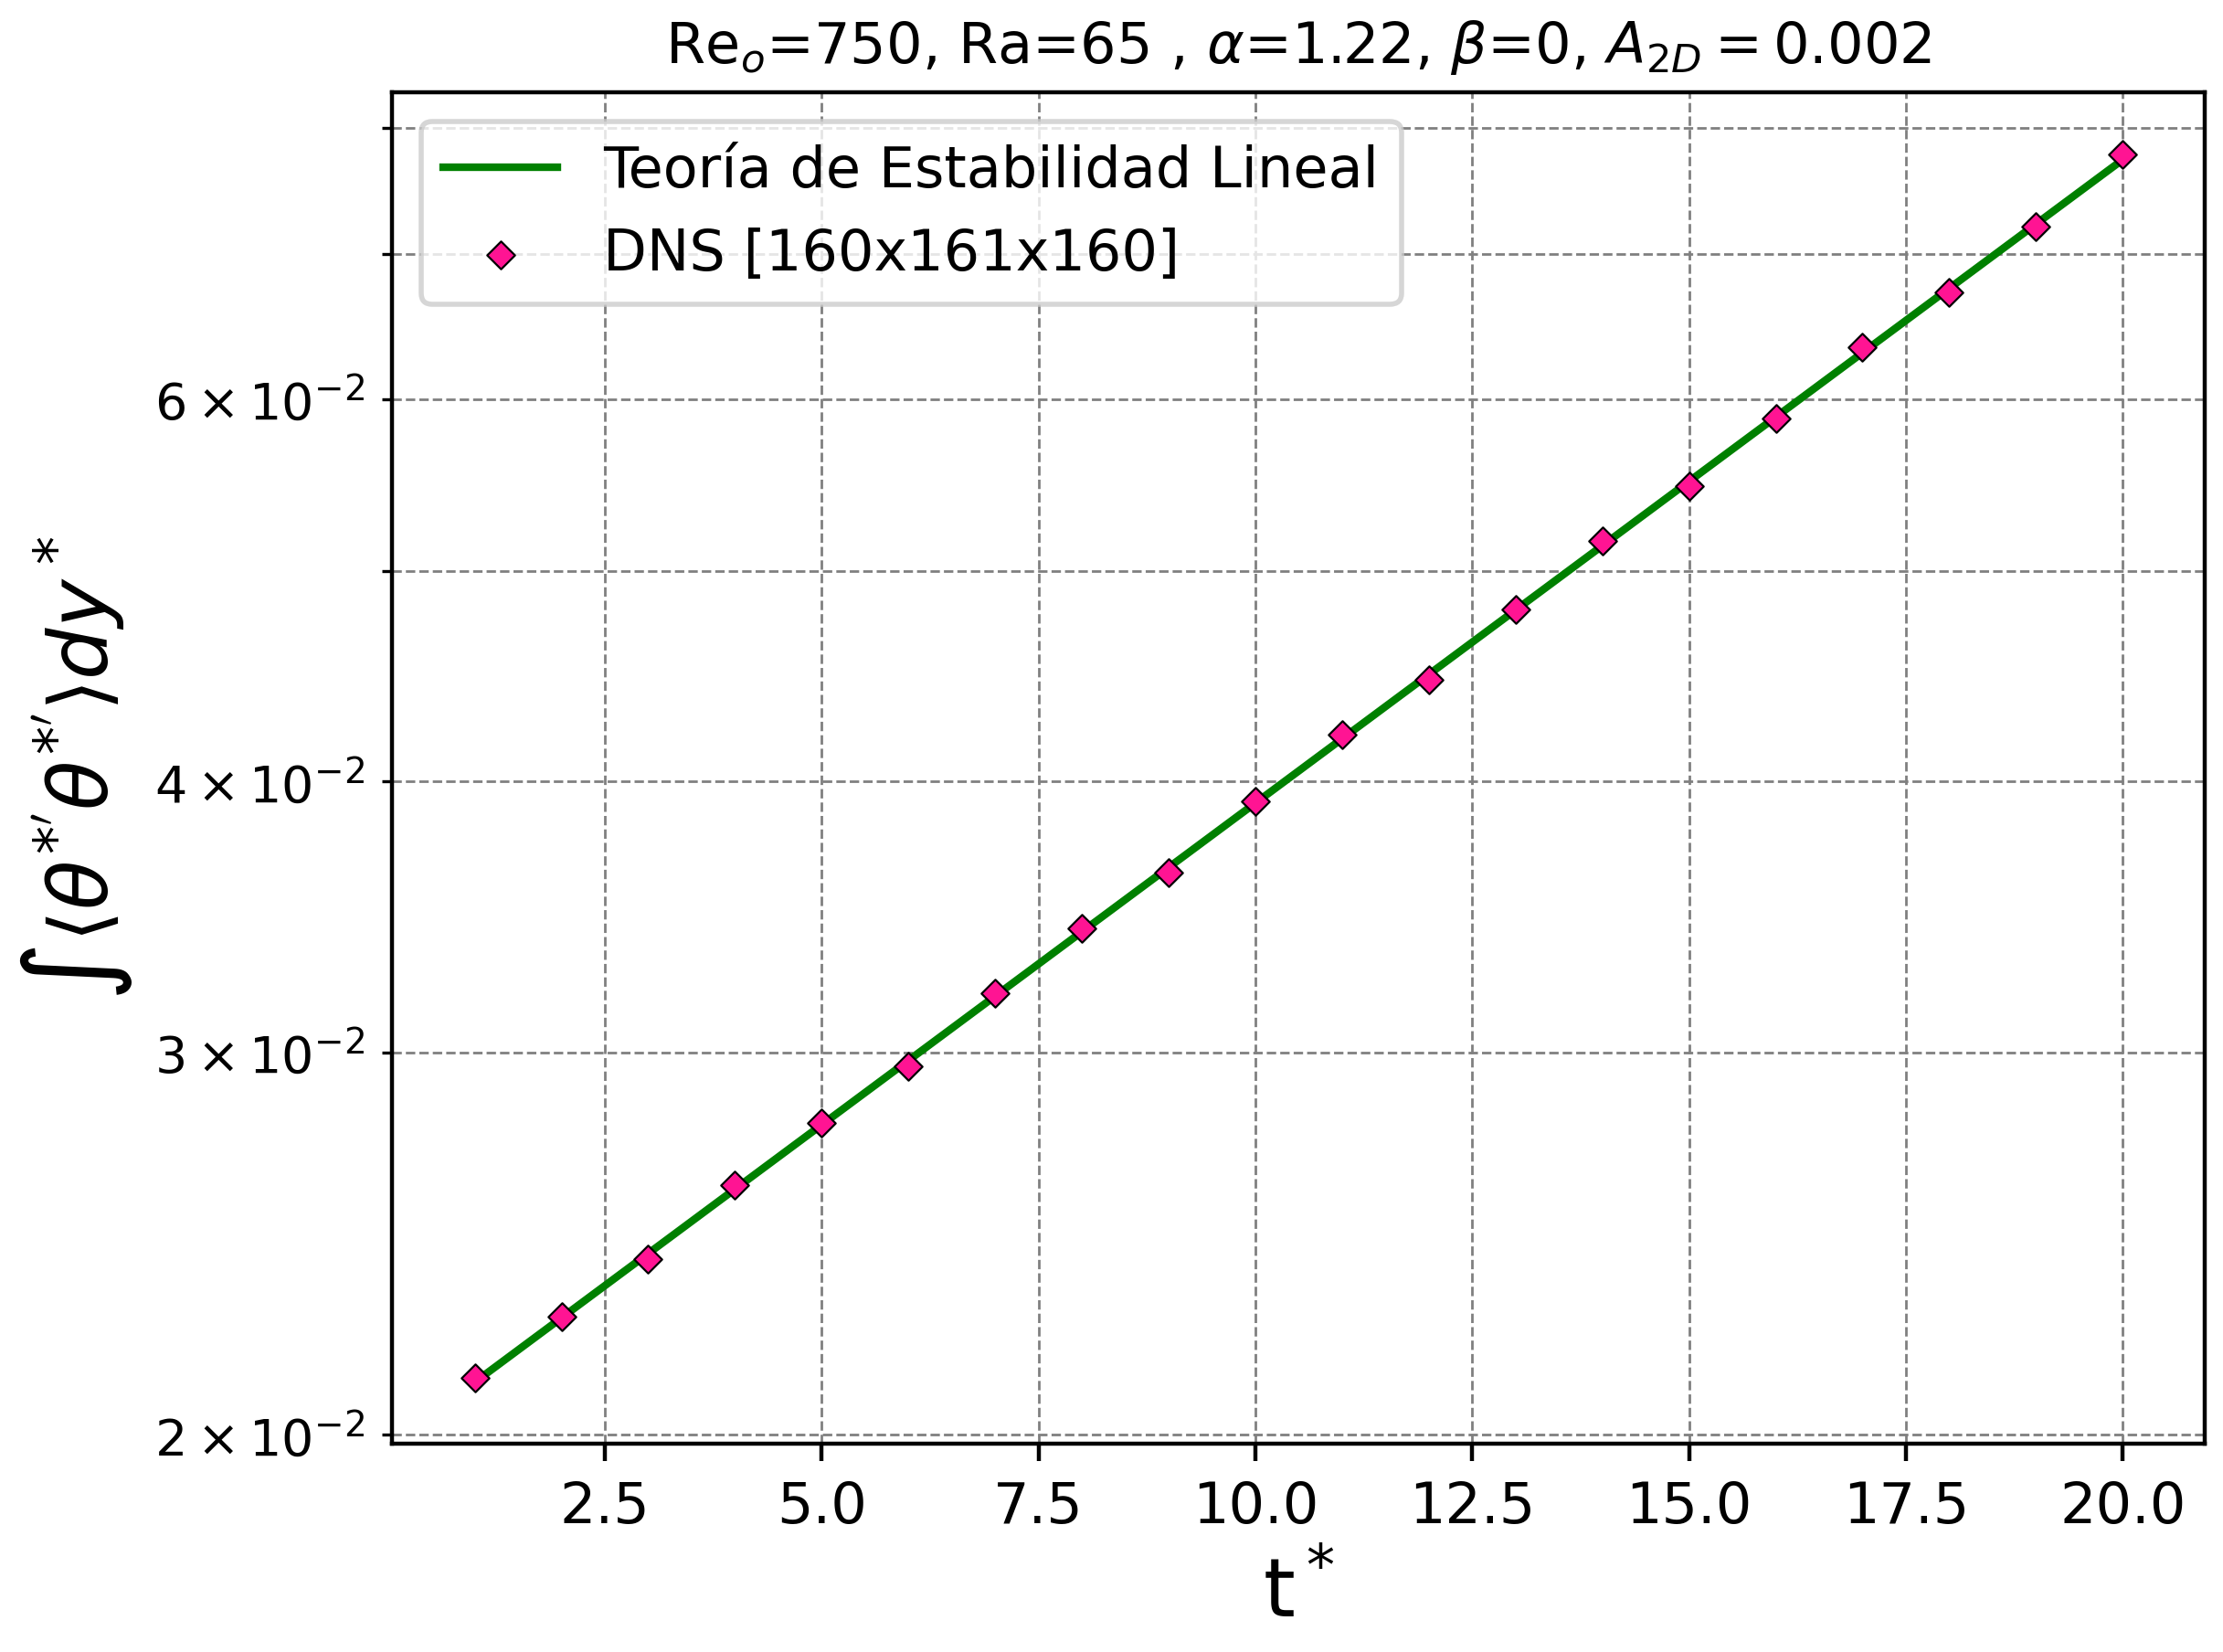
\includegraphics[width=0.49\textwidth]{figures/cap4/osmc/Ra65_RamaDer/theta_var.png}
    	 \label{fig:Ra65RD-tvar}}  
 \caption{Evolución temporal de la TKE y de la varianza de la temperatura del caso RD.} 
 \label{fig:Ra65R-DI}
\end{figure}

\begin{figure}[H]
 \centering
  \subfloat[]{
    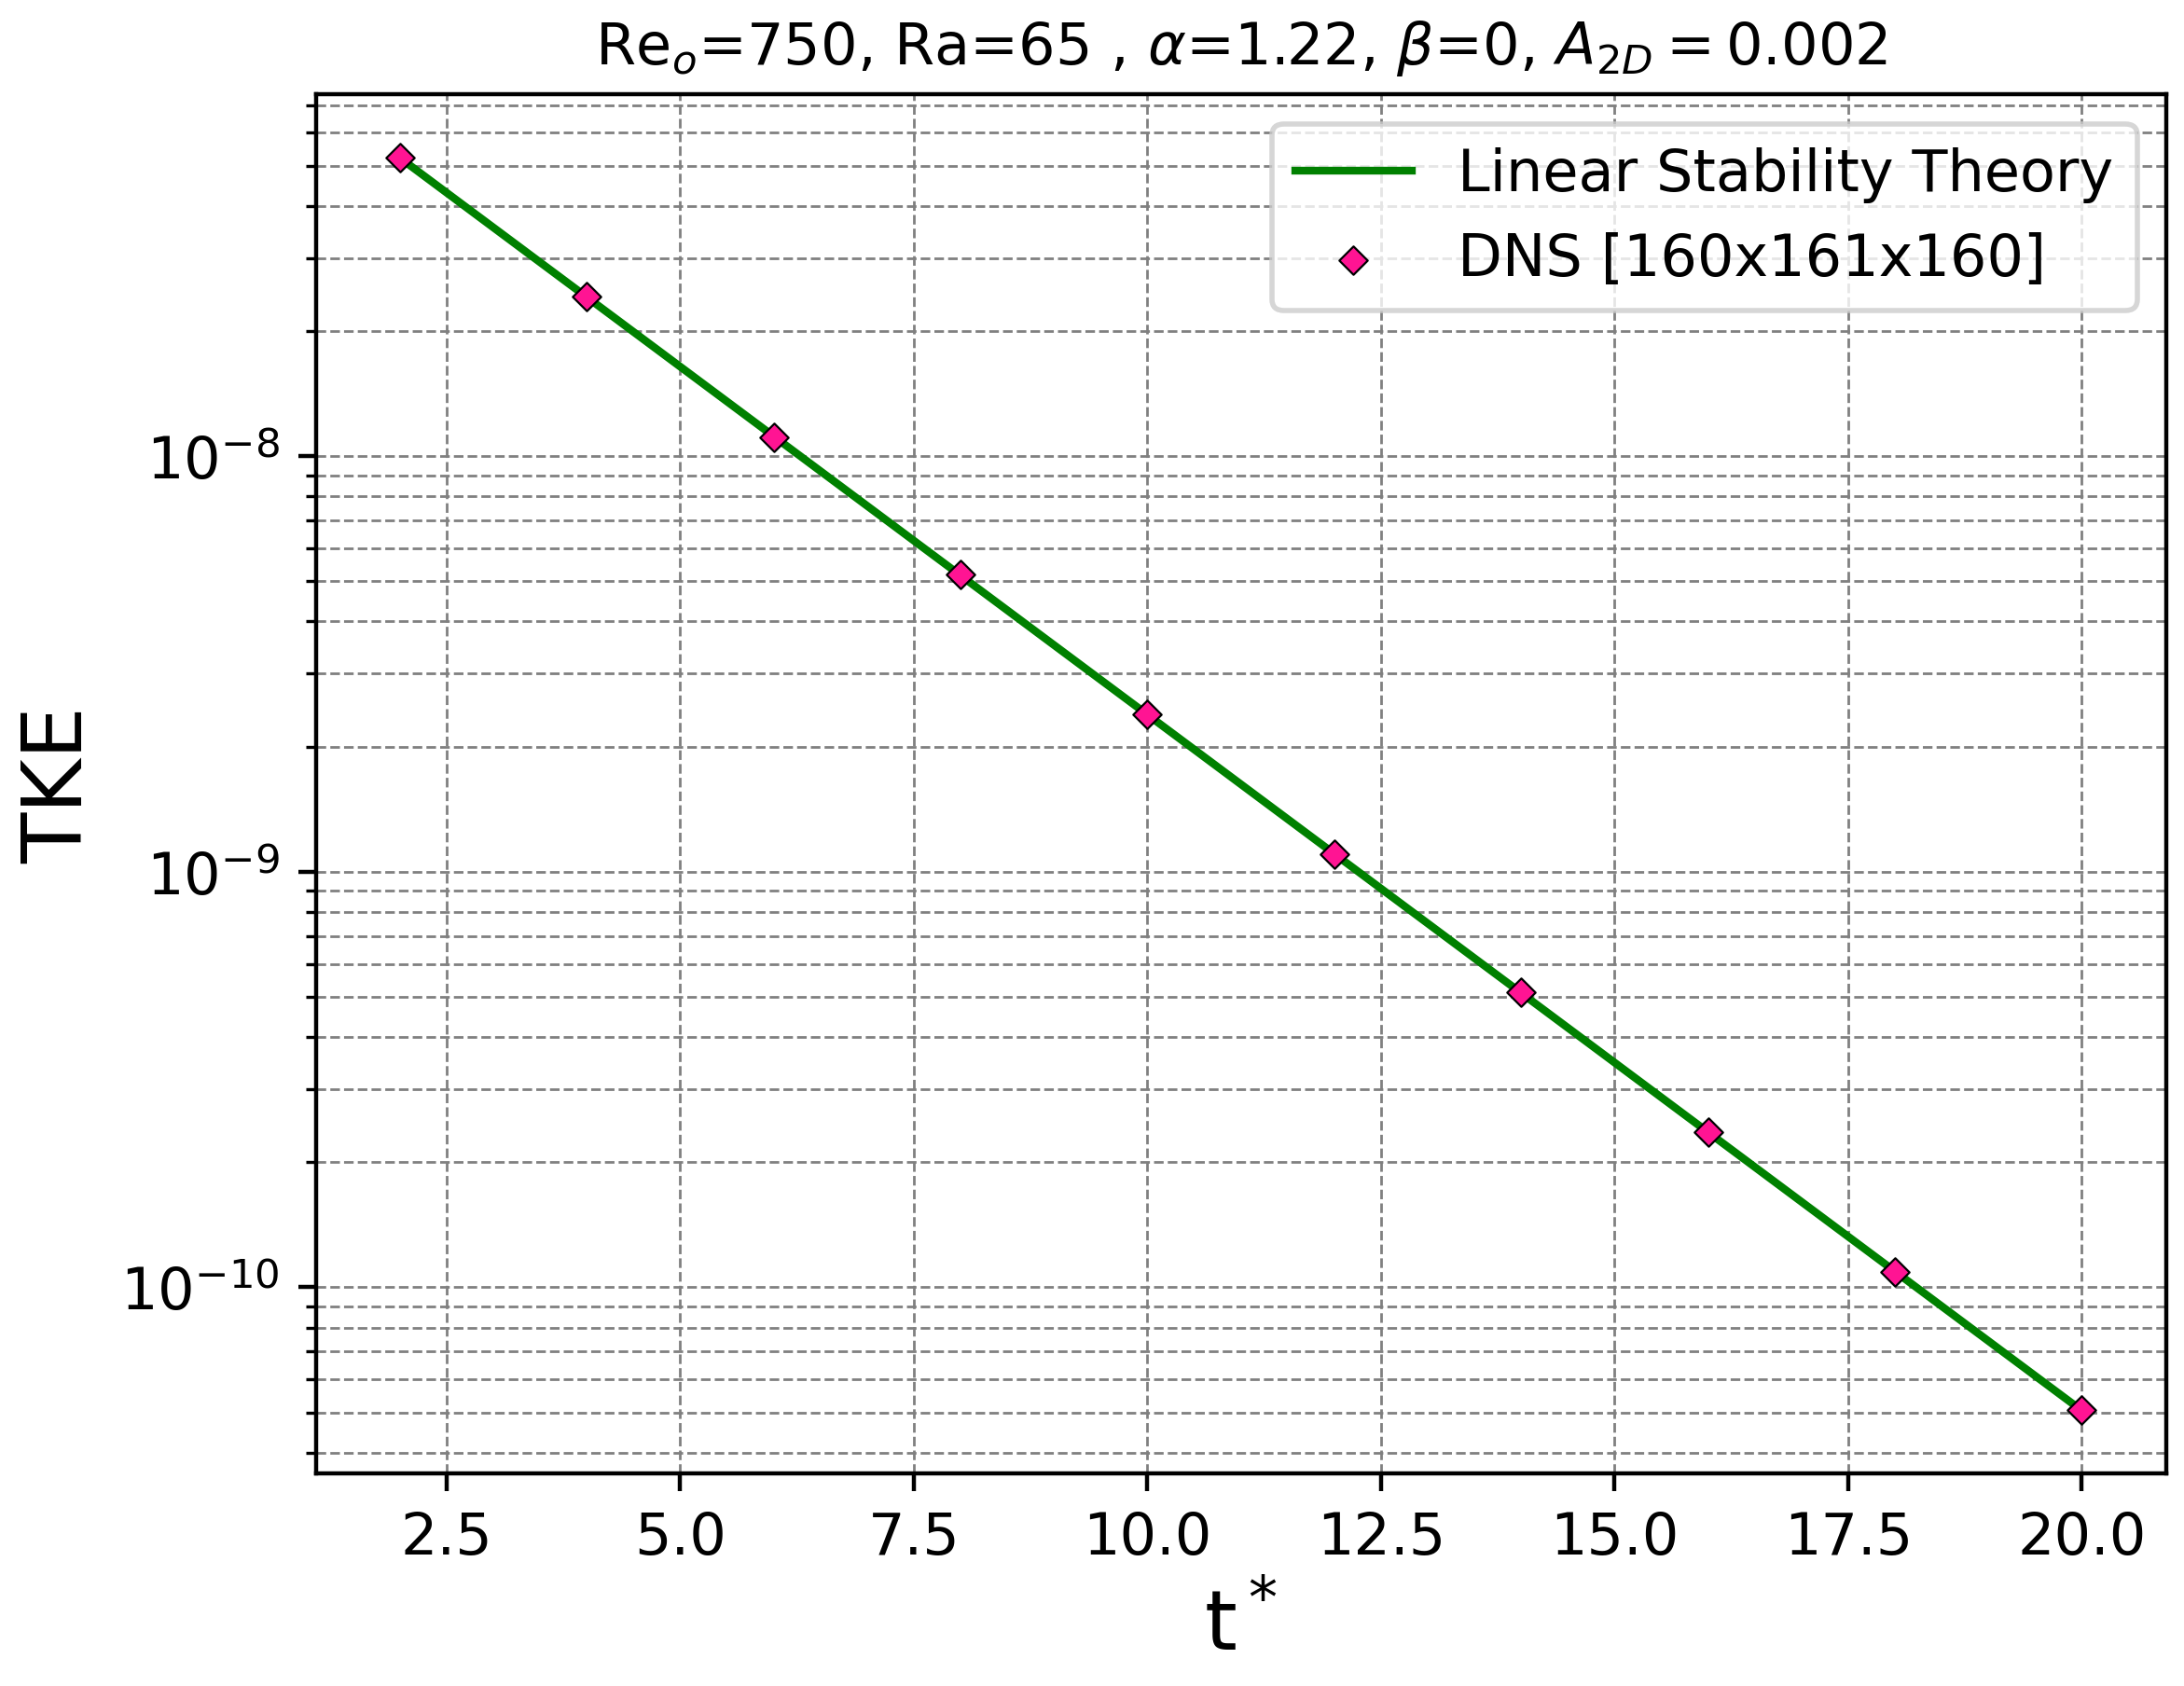
\includegraphics[width=0.49\textwidth]{figures/cap4/osmc/Ra65_RamaIzq/tke.png}
    	\label{fig:Ra65RI-tke}}  
  \subfloat[]{
    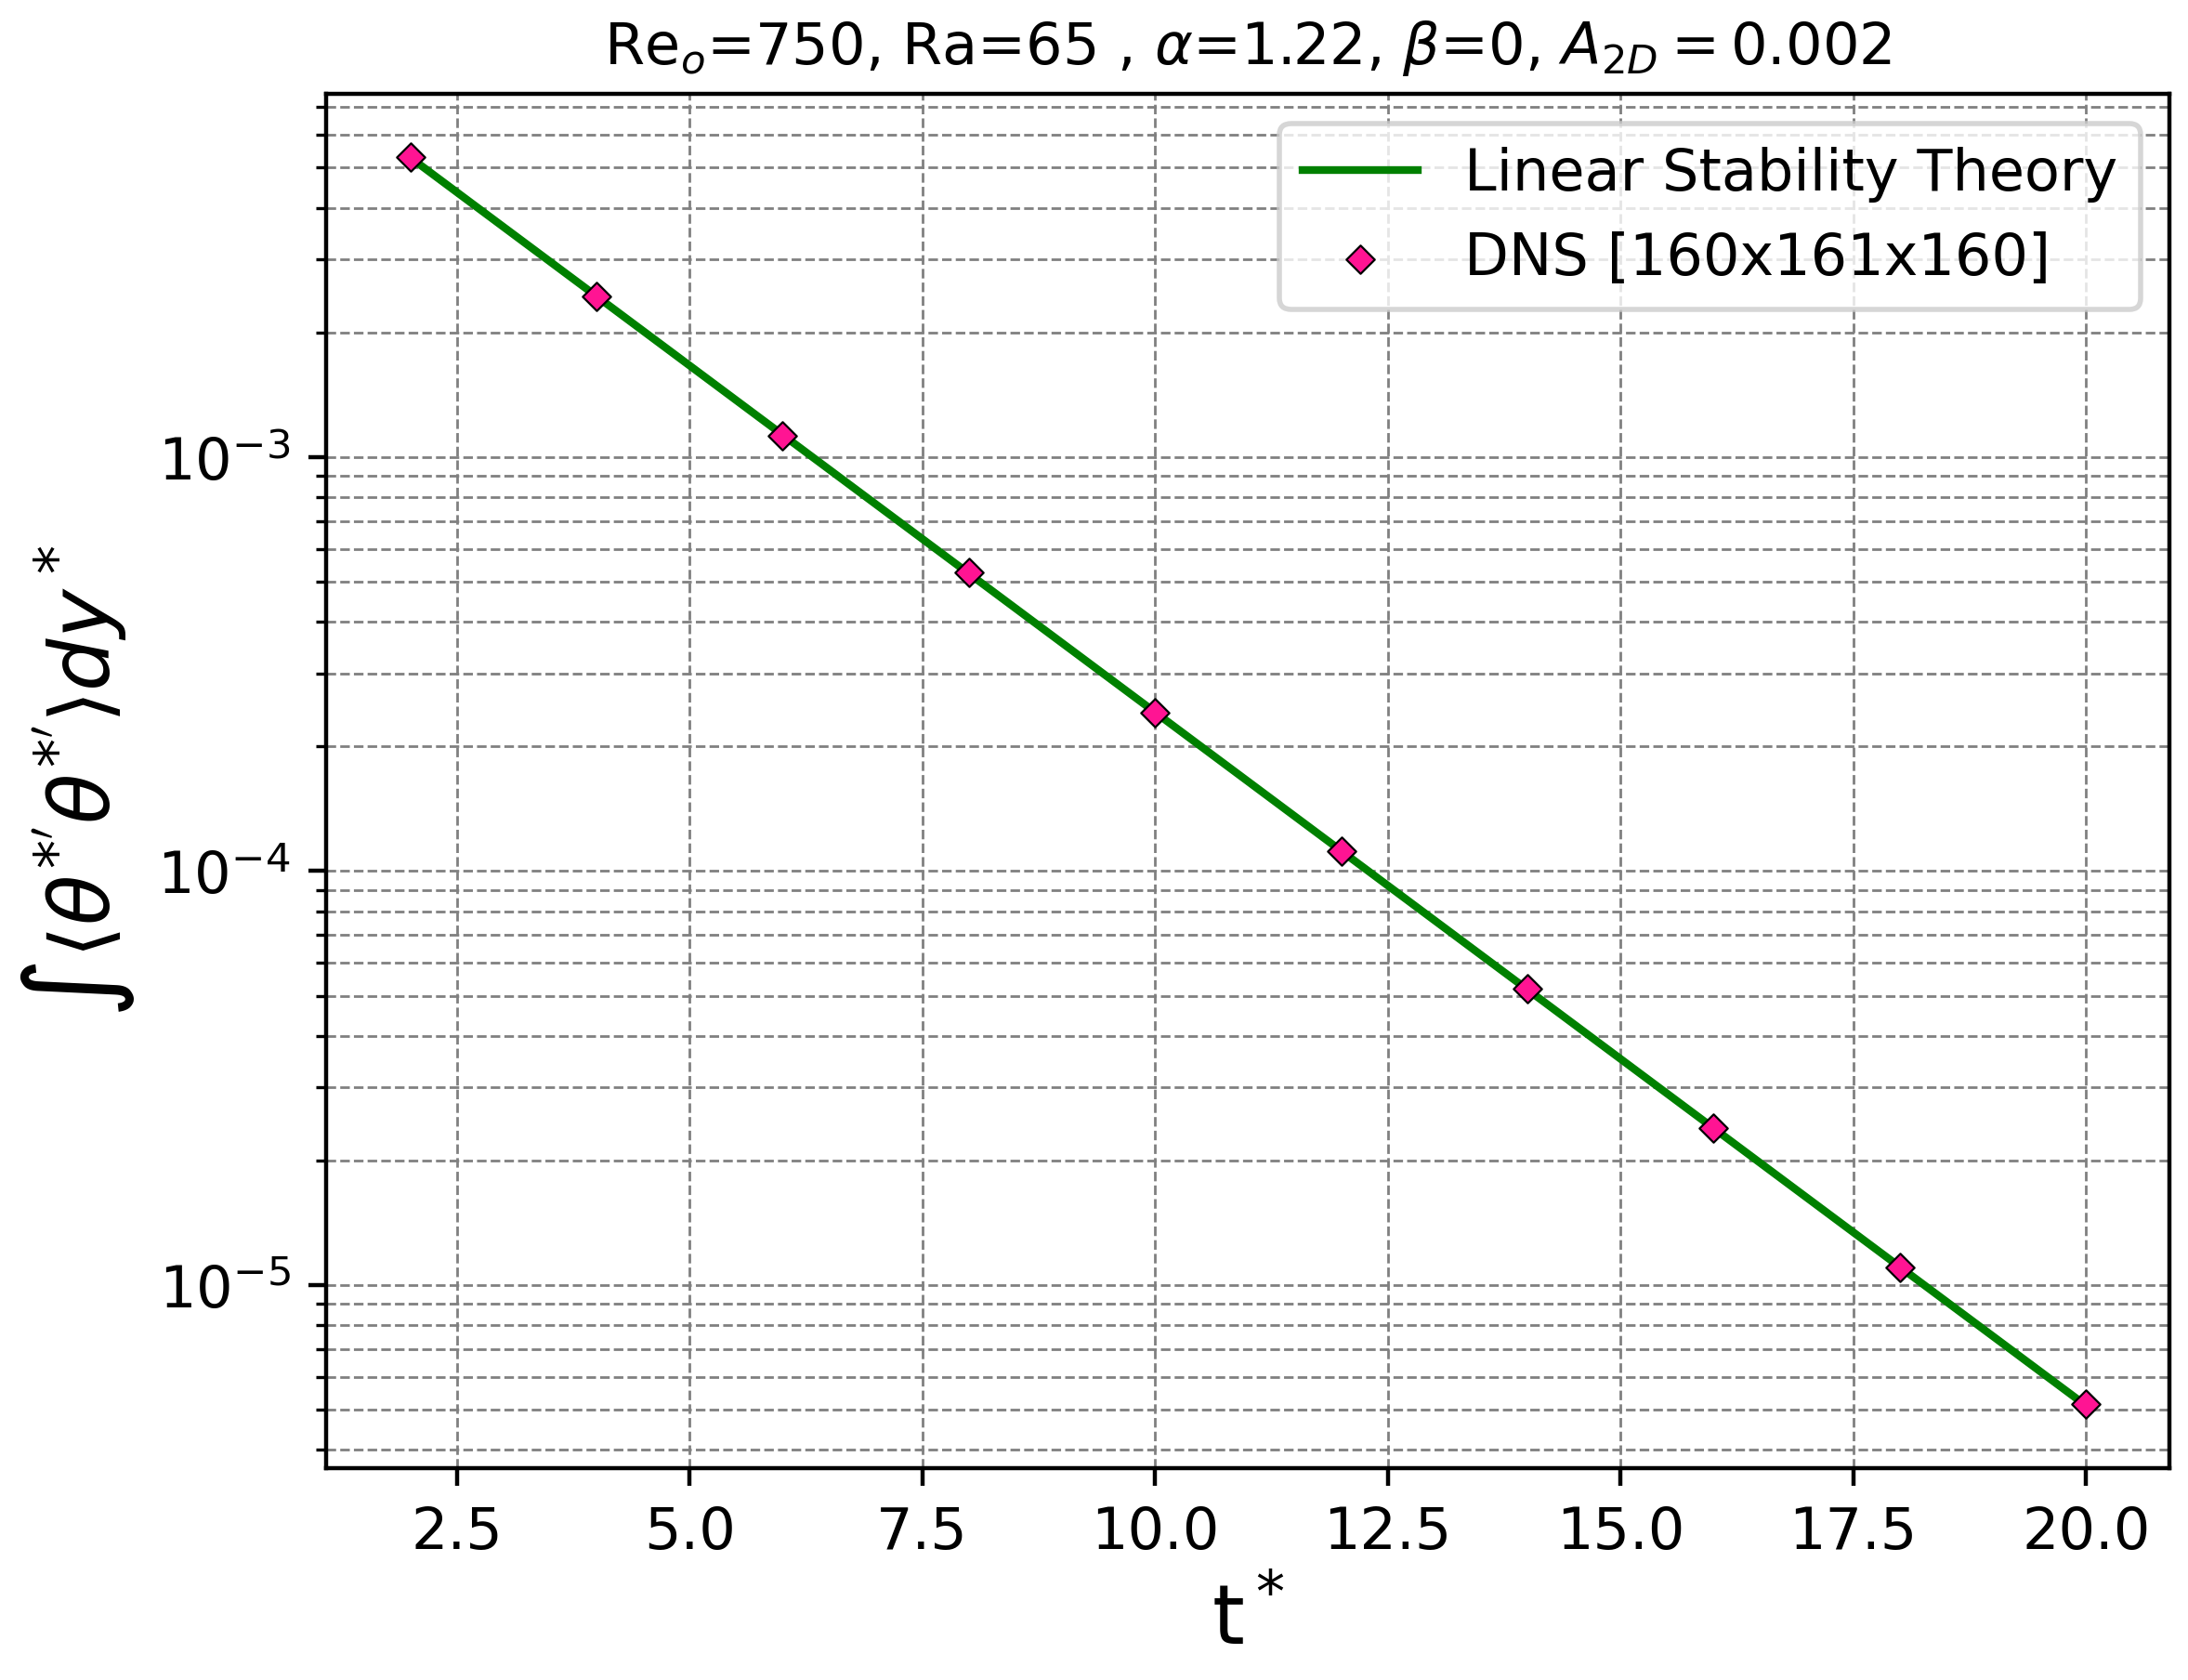
\includegraphics[width=0.49\textwidth]{figures/cap4/osmc/Ra65_RamaIzq/theta_var.png}
         \label{fig:Ra65RI-tvar}}  
 \caption{Evolución temporal de la TKE y de la varianza de la temperatura del caso RI.} 
 \label{fig:Ra65R-DI}
\end{figure}

Finalmente, se puede aseverar que la herramienta OSMC desarrollada por Szuban \linebreak \cite{szuban2023} es adecuada para imponer perturbaciones basadas en la teoría de estabilidad lineal. Por su parte, la herramienta numérica Xcompact3D produce resultados que se encuentran en consistencia con aquellos predichos por la teoría antes mencionada. Esto permite realizar el estudio de la transición temporal laminar-turbulenta que se lleva a cabo en el Capítulo \ref{cap:transicion}.

\chapter{Convección Mixta en Flujos Completamente Desarrollado}


El propósito de este capítulo es mostrar, vía simulaciones, cómo la flotabilidad o boyancia modifica un flujo turbulento plenamente desarrollado en un canal de placas paralelas. Se parte de simulaciones DNS que cubren un amplio espectro de números de Reynolds, Richardson y Prandtl, lo que permite examinar la transición desde convección forzada hasta convección natural. Tras describir los casos y las variables adimensionales de referencia, se presentan (i) magnitudes estadísticas de primer y segundo orden, (ii) la influencia del Prandtl sobre las subcapas viscosa y térmica, (iii) la variación del número de Nusselt y (iv) el impacto en el factor de fricción de Darcy.

\newpage

\section{Casos simulados} 

Los resultados de las simulaciones realizadas en este capítulo corresponden a un flujo completamente desarrollado tanto térmica como hidrodinámicamente. Se emplearon Re$_o$=2100, 3150, 4278, 5000, Pr=0.071, 0.71 y valores de Richardon en el rango 0.04 $\lesssim$ Ri$_b$ $\lesssim$ 106. En la Figura \ref{fig:map_flow_regime} se expone un ``mapa'' del régimen de flujo donde se gráfica el número de Reynolds\footnote{Número de Reynolds basado en el diámetro hidráulico: $Re^D_b = 8/3 \hspace*{1mm} Re_o$} versus el número de Richardson. De acuerdo al diagrama de Moody \cite{white}:

\begin{itemize}
	\item para valores de Re$^D_b$ $<$ 2000 el régimen es laminar,
	\item si 2000 $\lesssim$ Re$^D_b$ $\lesssim$ 4000 el régimen es de transición,
	\item y si Re$^D_b>$ 4000 el régimen es turbulento.
\end{itemize}
Por otra parte, el fenómeno de convección es \cite{incropera,cengelheat}:

\begin{itemize}
	\item forzado si Ri$_b<$ 0.1,
	\item mixto si 0.1 $<$ Ri$_b$ $<$10,
	\item y natural si Ri$_b$ $>$10.
\end{itemize}

\begin{figure}[H]
  \centering
    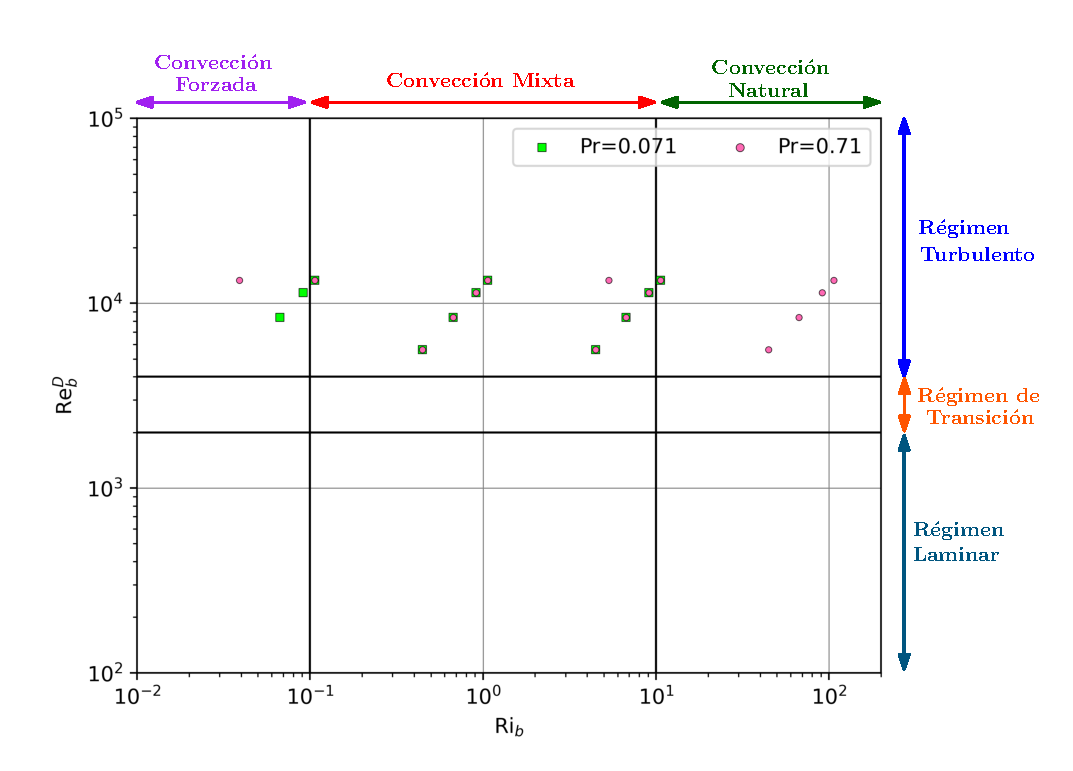
\includegraphics[width=0.8\textwidth]{figures/cap5/map.eps}
  \caption{Mapa de regímenes en el plano $Re_D$–$Ri_b$. Se señalan las zonas laminar, de transición y turbulenta, así como los dominios de convección forzada, mixta y natural.}
  \label{fig:map_flow_regime}
\end{figure}

La totalidad de casos se encuentra en un régimen de flujo turbulento. En su mayoría, los casos se encuentran en flujo de convección mixta, sin embargo, se cuenta con casos donde predomina la convección forzada, y por otro lado, donde domina la convección natural. Esto brinda un espectro más amplio para el análisis del problema.









\section{Magnitudes de Primer y Segundo Orden}

En esta sección, se analiza la influencia de la fuerza boyante en las magnitudes estadísticas de primer y segundo orden. Para tal fin, se consideran, únicamente, los casos Re$_o$=5000 y Pr=0.71. El aumento de la fuerza boyante, o el número de Ri$_b$, equivale a aumentar el flujo de calor ya que Ri$_b$ es proporcional al flujo de calor $q''_w$. En otras palabras, el aumento de la boyancia en el sistema físico corresponde a aumentar la energía térmica que se le entrega a través de las paredes cuando el fluido es ascendente\footnote{También es equivalente a quitarle energía térmica (enfriar las paredes) cuando la dirección del flujo es descendente.}.


\subsection{Perfiles de velocidad y de temperatura} \label{sec:velo_temp}

En la Figura \ref{fig:ux-Re5000-Pr071} se presentan los perfiles promedio de velocidad en la dirección \textit{streamwise} para distintos números de Richardson. En dichos perfiles pueden distinguirse con claridad los tres regímenes de convección. Conforme se intensifica la fuerza boyante, las curvas adoptan una configuración en ``M'', en concordancia con lo reportado por otros autores \cite{you2003direct, zhou2024direct}. A diferencia del caso de convección exclusivamente forzada, el máximo de velocidad deja de situarse en la línea central del canal y se desplaza progresivamente hacia la pared a medida que aumenta Ri$_b$,\cite{carr1973velocity, steiner1971reverse, zhou2024direct}, originando dos máximos locales en lugar del único pico característico del flujo puramente forzado. Este comportamiento puede interpretarse cualitativamente del siguiente modo: en las proximidades de la pared el fluido se encuentra a mayor temperatura lo que implica menor densidad; en consecuencia, la fuerza boyante acelera el flujo en esa región y, por conservación de masa, el fluido ubicado en la zona central experimenta una desaceleración.

\begin{figure}[H]
  \centering
  \subfloat[]{
    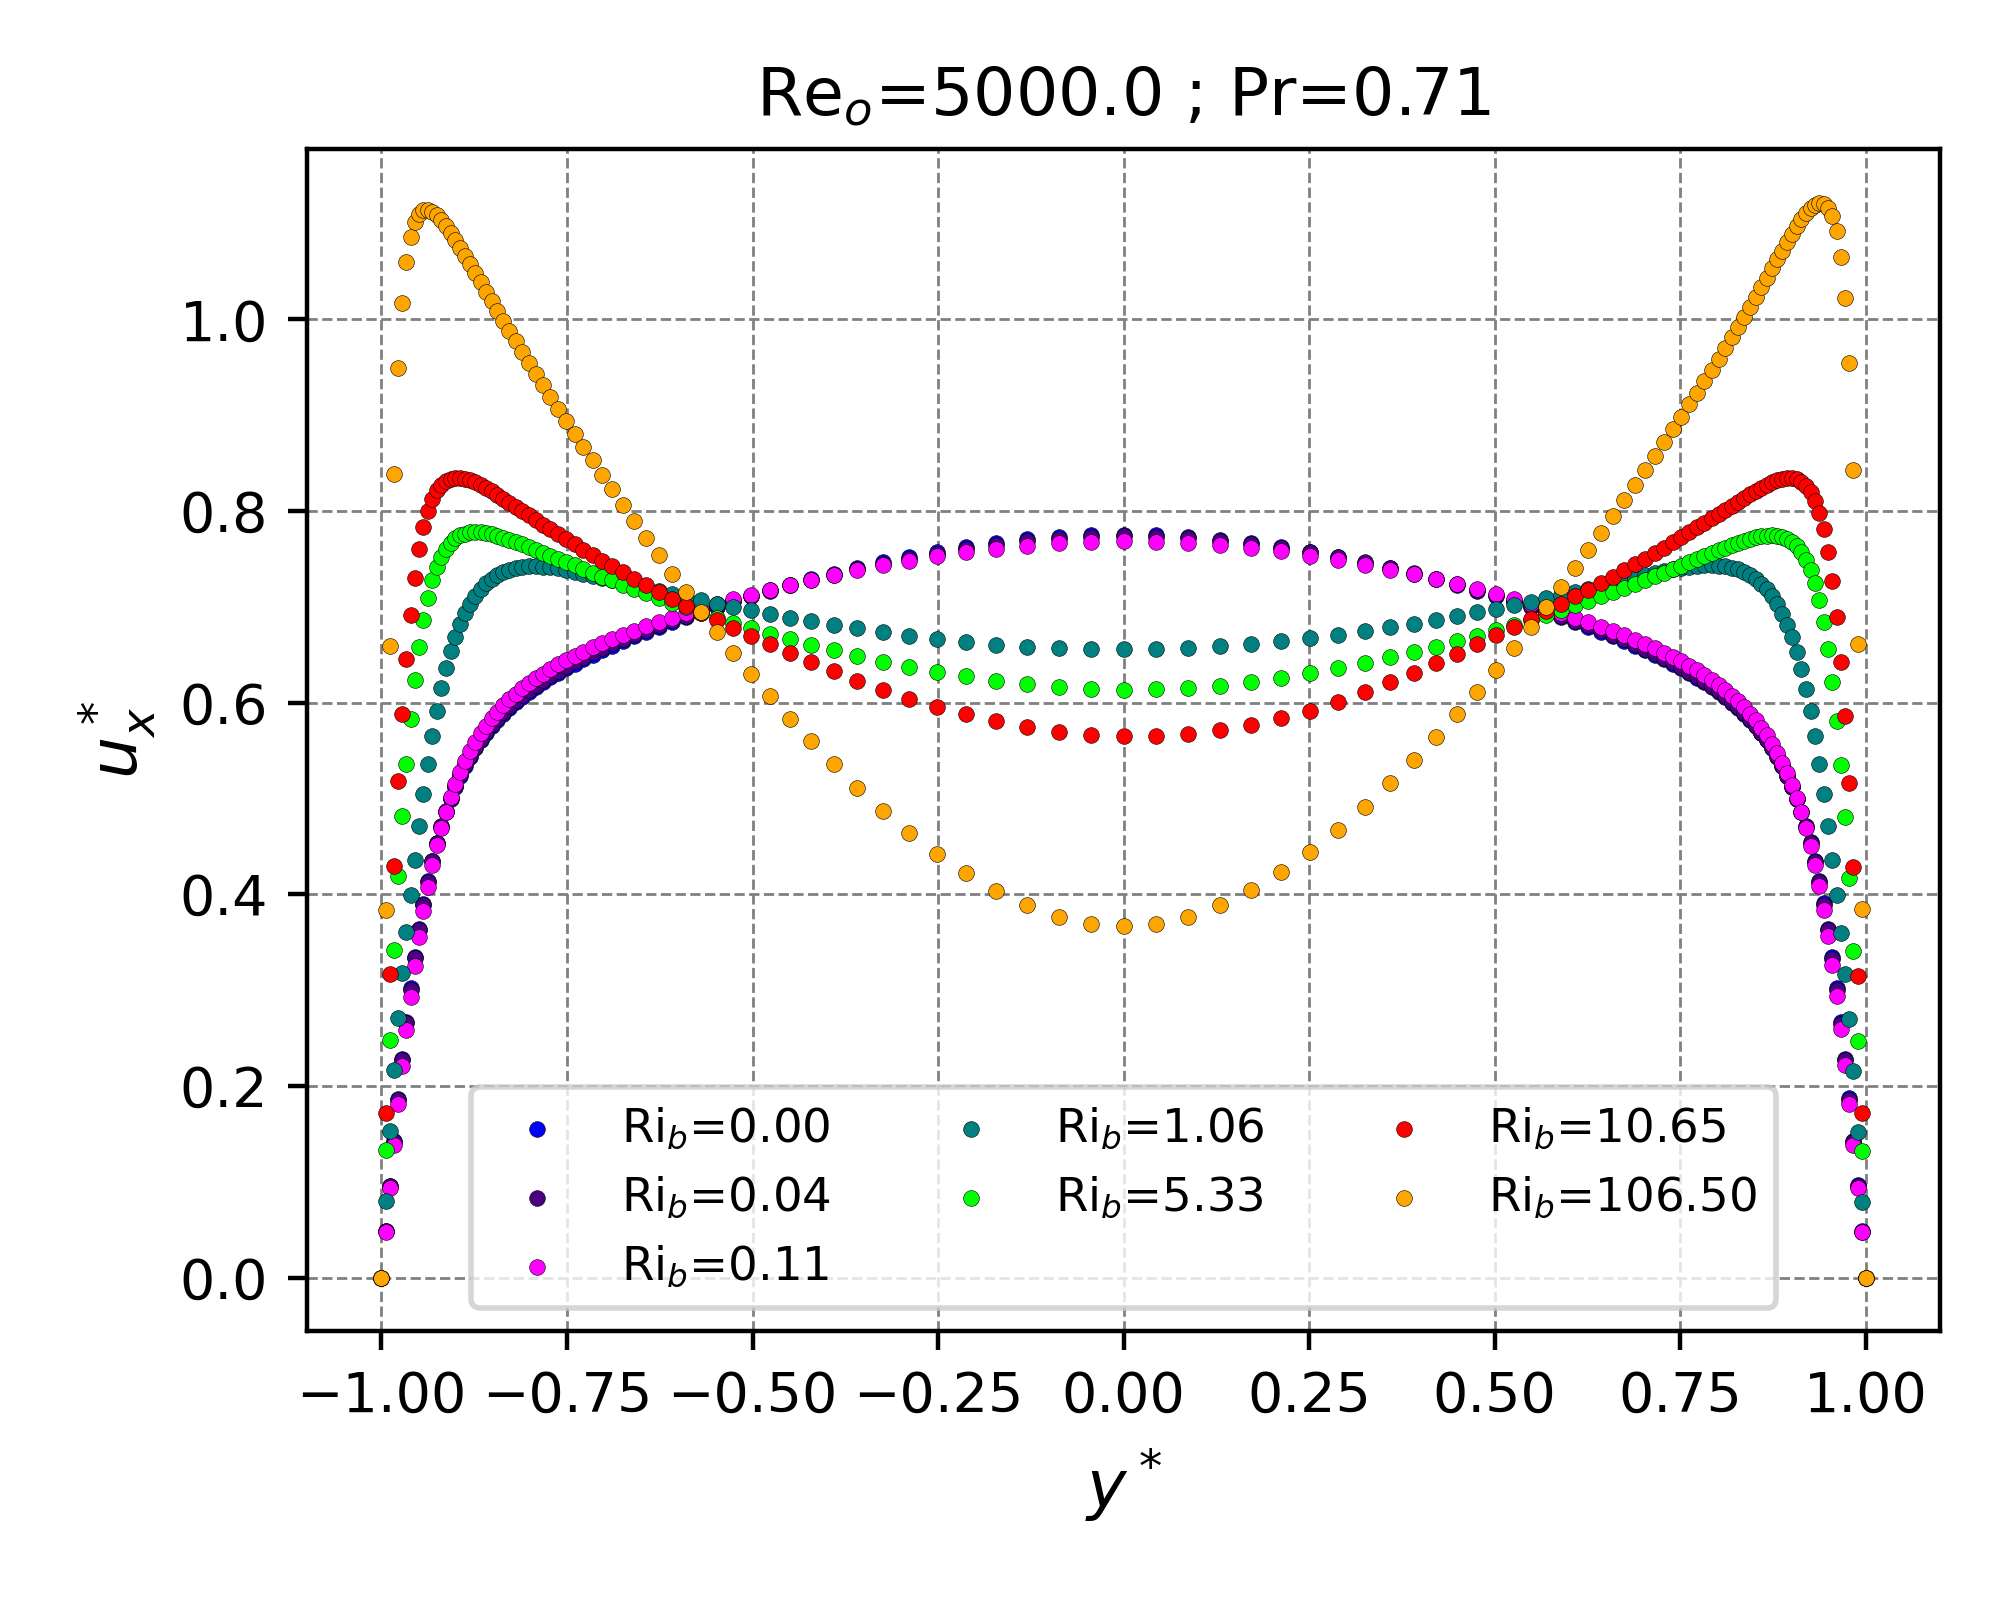
\includegraphics[width=0.49\textwidth]{figures/cap5/Re5000-Pr071/ux_mean_profile.png}
    	\label{fig:ux-Re5000-Pr071}}
  \subfloat[]{
    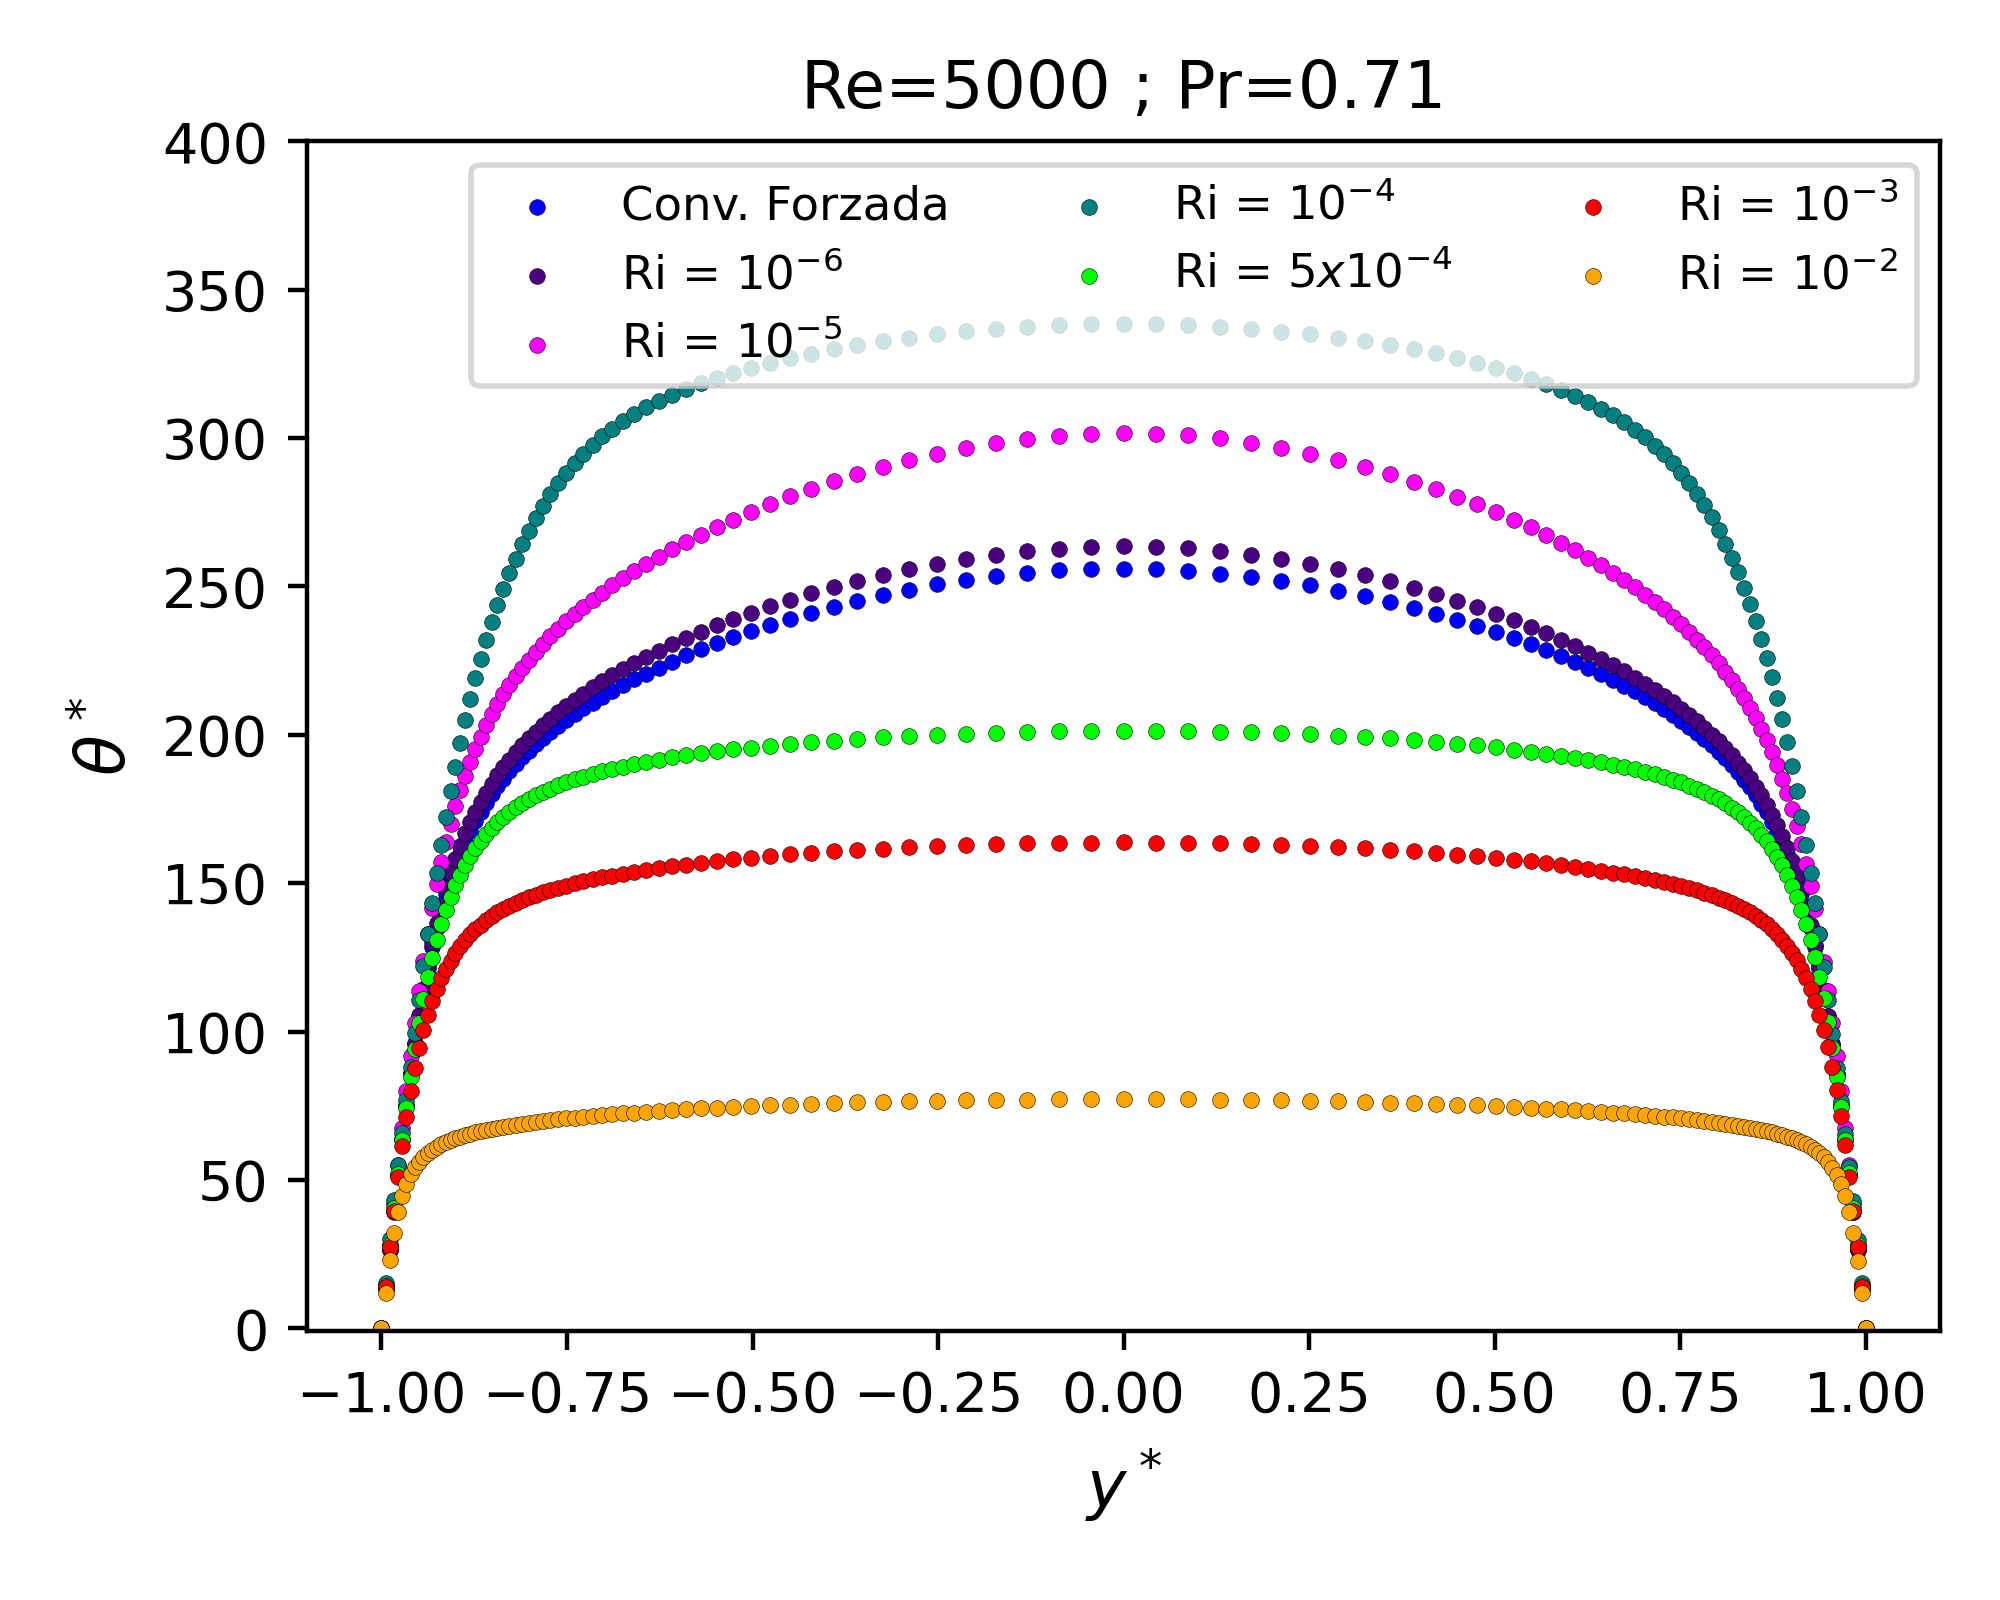
\includegraphics[width=0.49\textwidth]{figures/cap5/Re5000-Pr071/phi_mean_profile.png}
    	\label{fig:phi-Re5000-Pr071}}
  \caption{Perfiles medios adimensionales de \textbf{(a)} velocidad y \textbf{(b)} temperatura, para varios Ri$_b$.}
\end{figure}

%Por otra parte, la Figura \ref{fig:phi-Re5000-Pr071} se exponen los perfiles medios de temperatura adimensional. Al contrario que los perfiles de velocidad, aquí no presentan una forma en ``M'' \cite{you2003direct, steiner1971reverse}. Aquí, los casos se pueden dividir, a priori, en dos grupos: el primer grupo que corresponde a valores de Rib$_b$ entre 0.04 y 1.06, y el segundo grupo está compuesto por valores de 5.33 a 106.5. En el primer grupo, se observa el crecimiento de los perfiles, correspondiente a un decrecimiento en el perfil de temperatura real del sistema. A medida que incrementa la fuerza boyante, como se observa en el segundo grupo, la temperatura adimensional decrece y ello significa un crecimiento en el perfil de temperatura real. Por otro lado, la forma ``achatada'' puede explicarse cualitativamente con ayuda de los perfiles de velocidad. La diferencia de velocidades entre las zonas cercanas a la pared y el centro del canal promueven la mezcla del fluido y con ello una distribución más homogénea de la temperatura. 
%
%Como se verá en la sección \ref{sec:nu}, en el primer grupo, la transferencia de calor por convección empeora y en el segundo grupo, la misma se recupera y mejora.
%
%Estas afirmaciones, que no son evidentes a primera vista, se comprenden a partir de la Figura \ref{fig:uphi-Re5000-Pr071}, donde se muestra el perfil medio $\langle u_x^{*} \theta^{*} \rangle$. El número de Nusselt es inversamente proporcional a
%$\langle \theta^*_b \rangle$ (ecuación \ref{eq:nu}), el cual depende del comportamiento de $\langle u_x^{*} \theta^{*} \rangle$. Así, un incremento de la temperatura aumenta $\langle u_x^{*} \theta^{*} \rangle$, y, en consecuencia, eleva $\langle \theta_b^{*} \rangle$, lo que provoca una disminución de Nu.



Por otra parte, la Figura \ref{fig:phi-Re5000-Pr071} presenta los perfiles medios de temperatura adimensional. A diferencia de los perfiles de velocidad, estos no exhiben la configuración en ``M'' al igual que reportan otros autores \cite{you2003direct, steiner1971reverse}. Los casos pueden clasificarse, en primera instancia, en dos conjuntos: (i) valores de Ri$_b$ comprendidos entre 0.04 y 1.06, y (ii) valores entre 5.33 y 106.5. En el primer conjunto se aprecia un aumento del perfil adimensional, lo que equivale a un descenso de la temperatura dimensional. Cuando la fuerza boyante se intensifica (segundo conjunto) la temperatura adimensional disminuye, indicando un incremento de la temperatura real del fluido. La forma ``achatada'' de estos perfiles puede interpretarse cualitativamente a partir de los perfiles de velocidad: la diferencia de velocidades entre la región próxima a la pared y el centro del canal favorece la mezcla del fluido y, por consiguiente, conduce a una distribución térmica más homogénea.

Como se analizará en la sección \ref{sec:nu}, en el primer conjunto la transferencia de calor por convección se deteriora, mientras que en el segundo conjunto dicha transferencia se recupera e incluso mejora. Estas observaciones, que no son evidentes a primera vista, se esclarecen al examinar la Figura \ref{fig:uphi-Re5000-Pr071}, donde se representa el perfil medio $\langle u_x^{*}\theta^{*}\rangle$. El número de Nusselt es inversamente proporcional a $\langle\theta^{*}_b\rangle$ (ecuación \ref{eq:nu}), magnitud que depende del comportamiento de $\langle u_x^{*}\theta^{*}\rangle$. En consecuencia, un aumento de la temperatura incrementa $\langle u_x^{*}\theta^{*}\rangle$ y, por lo tanto, eleva $\langle\theta^{*}_b\rangle$, lo que conlleva una disminución de Nu.

\begin{figure}[H] % usa [H] solo si necesitas anclarla y tienes \usepackage{float}
  \centering
  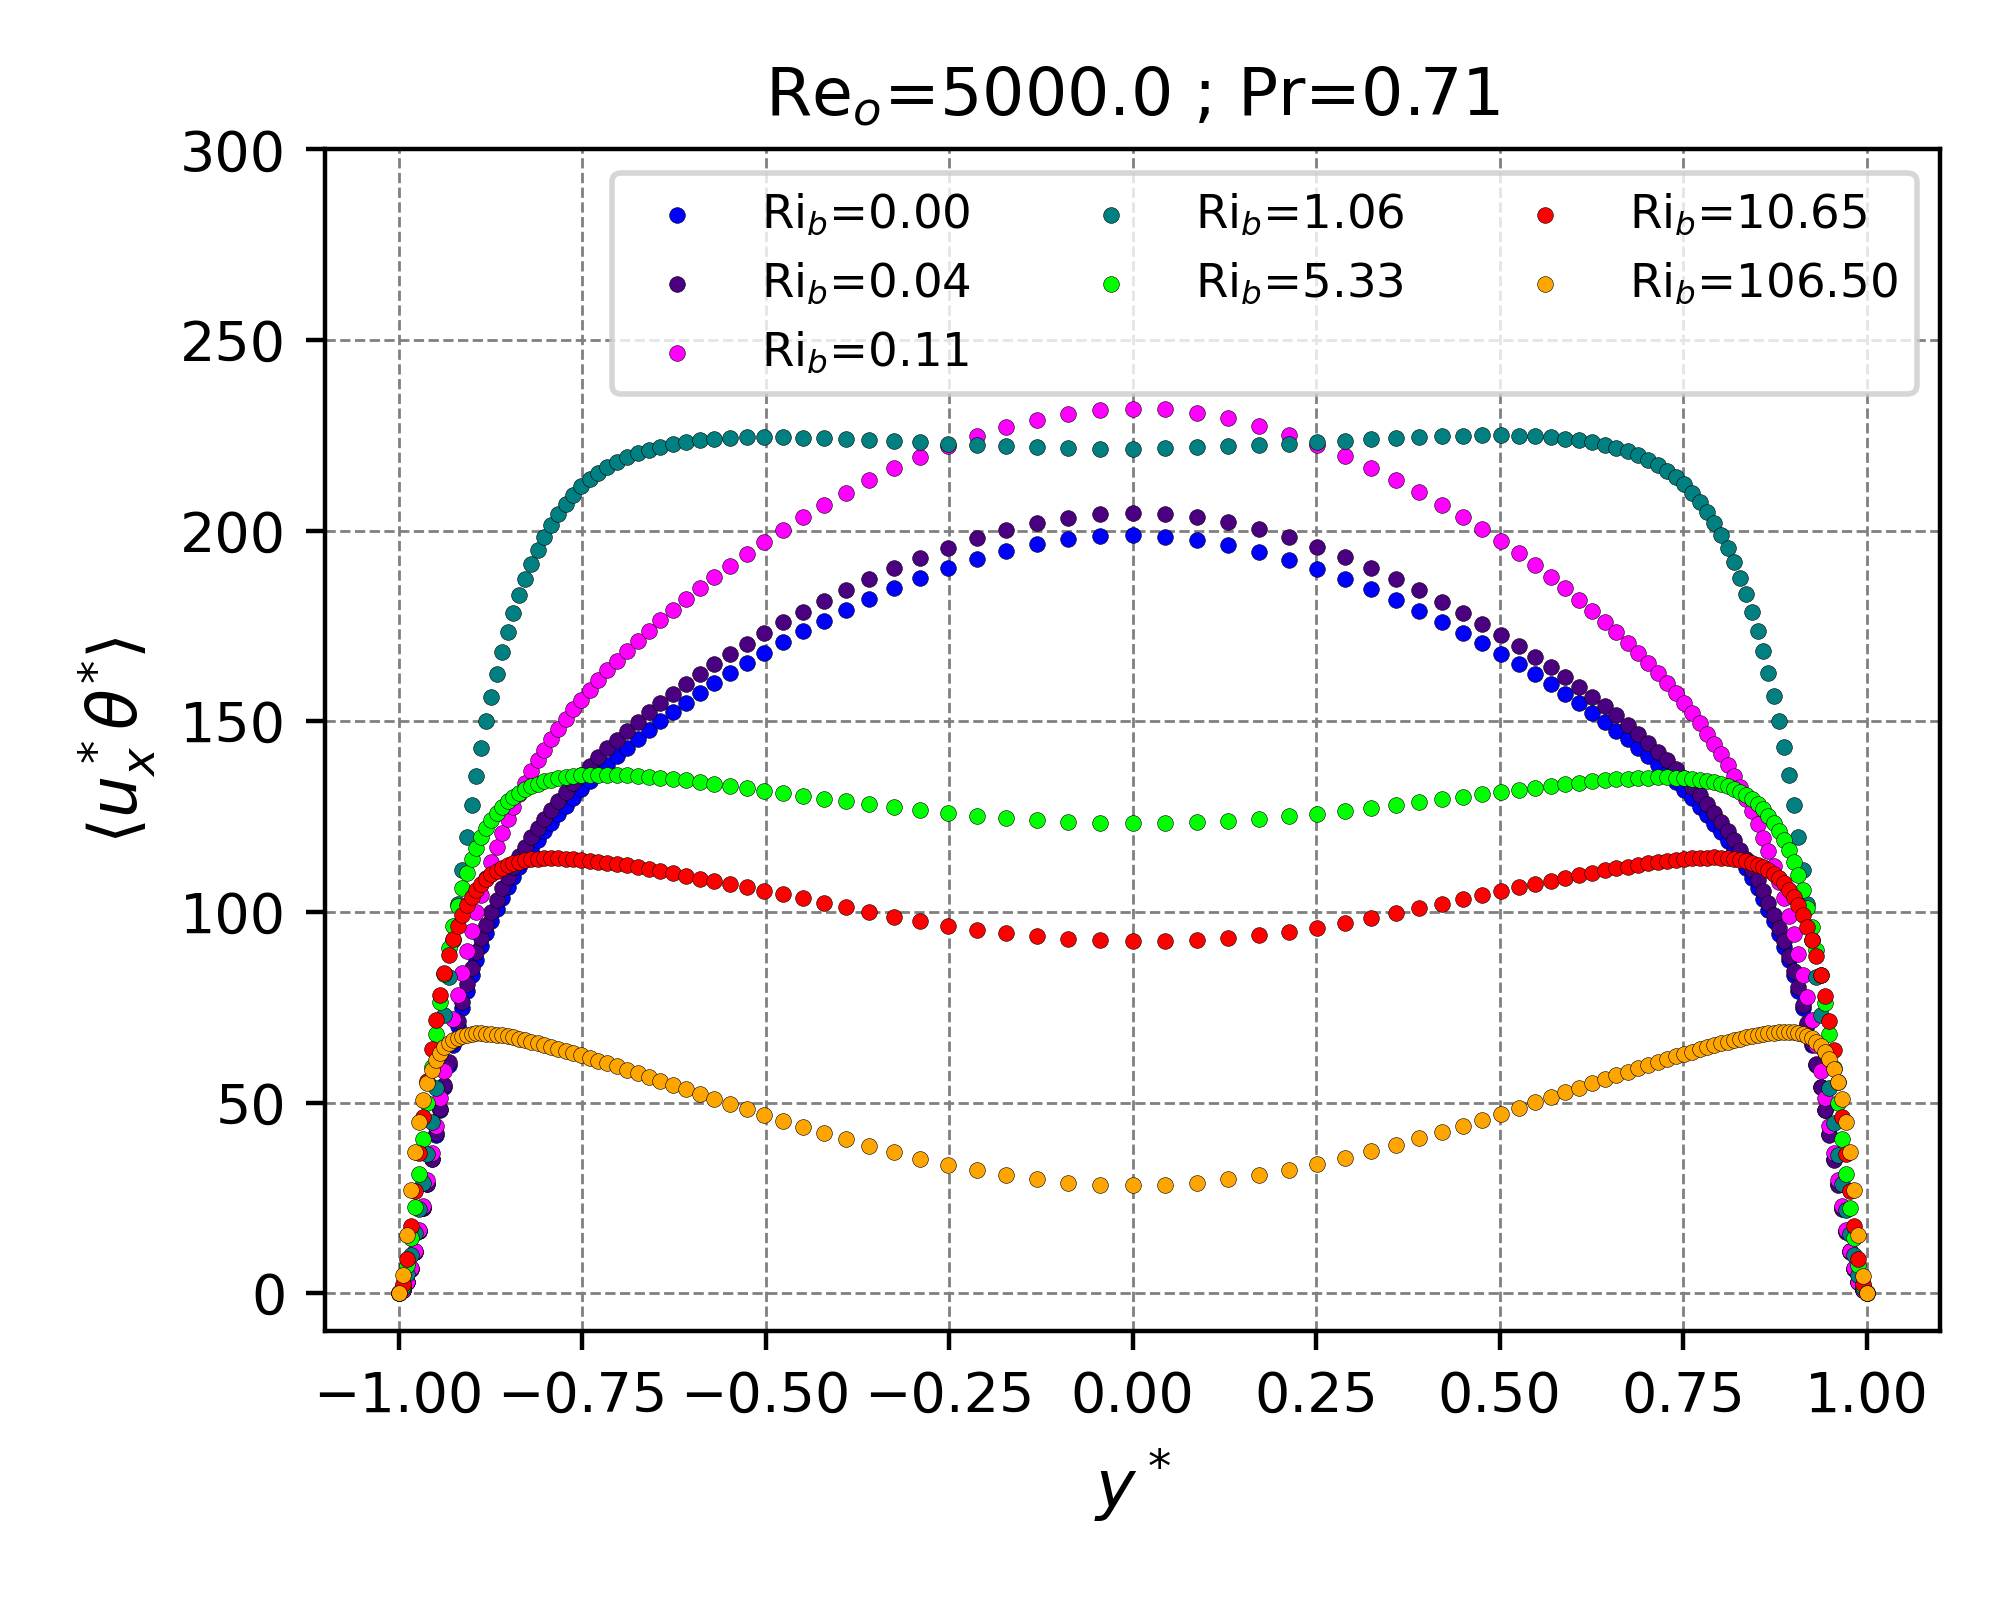
\includegraphics[width=0.6\textwidth]{figures/cap5/Re5000-Pr071/uphi_profile.png}
  \caption{Perfil de la magnitud media $\langle u^{*}_x\theta^{*}\rangle$.}
  \label{fig:uphi-Re5000-Pr071}
\end{figure}




\subsection{Valores RMS de temperatura, velocidad y flujo turbulento de calor} 

Las Figuras \ref{fig:rms-phi-log-Re5000-Pr071} y \ref{fig:rms-ux-Re5000-Pr071} muestran, respectivamente, los perfiles de las fluctuaciones de temperatura adimensional y de velocidad en la dirección \textit{streamwise}. A primera vista, al aumentar el número de Richardson, las fluctuaciones de temperatura disminuyen mientras que las de velocidad aumentan, lo cual se aprecia sobre todo en los casos de Ri$_b$ más elevados. No obstante, para Ri$_b = 0{.}04$, $0{.}11$ y $1{.}06$ la evolución difiere: primero se observa una reducción (incremento) de las fluctuaciones de velocidad (temperatura) seguida de una ligera recuperación (caída) antes de alinearse con la tendencia general del resto de los casos. Este comportamiento particular también fue encontrado en otros trabajos \cite{you2003direct,carr1973velocity}. El incremento de $(u_x^*)_{rms}$ con la fuerza boyante sugiere que el flujo adquiere un carácter más caótico, y por ende, más turbulento, lo que potencia la mezcla y genera mayor homogeneidad en la temperatura adimensional, y por tanto, atenúa las fluctuaciones de la misma.

\begin{figure}[H]
  \centering
  \subfloat[]{
    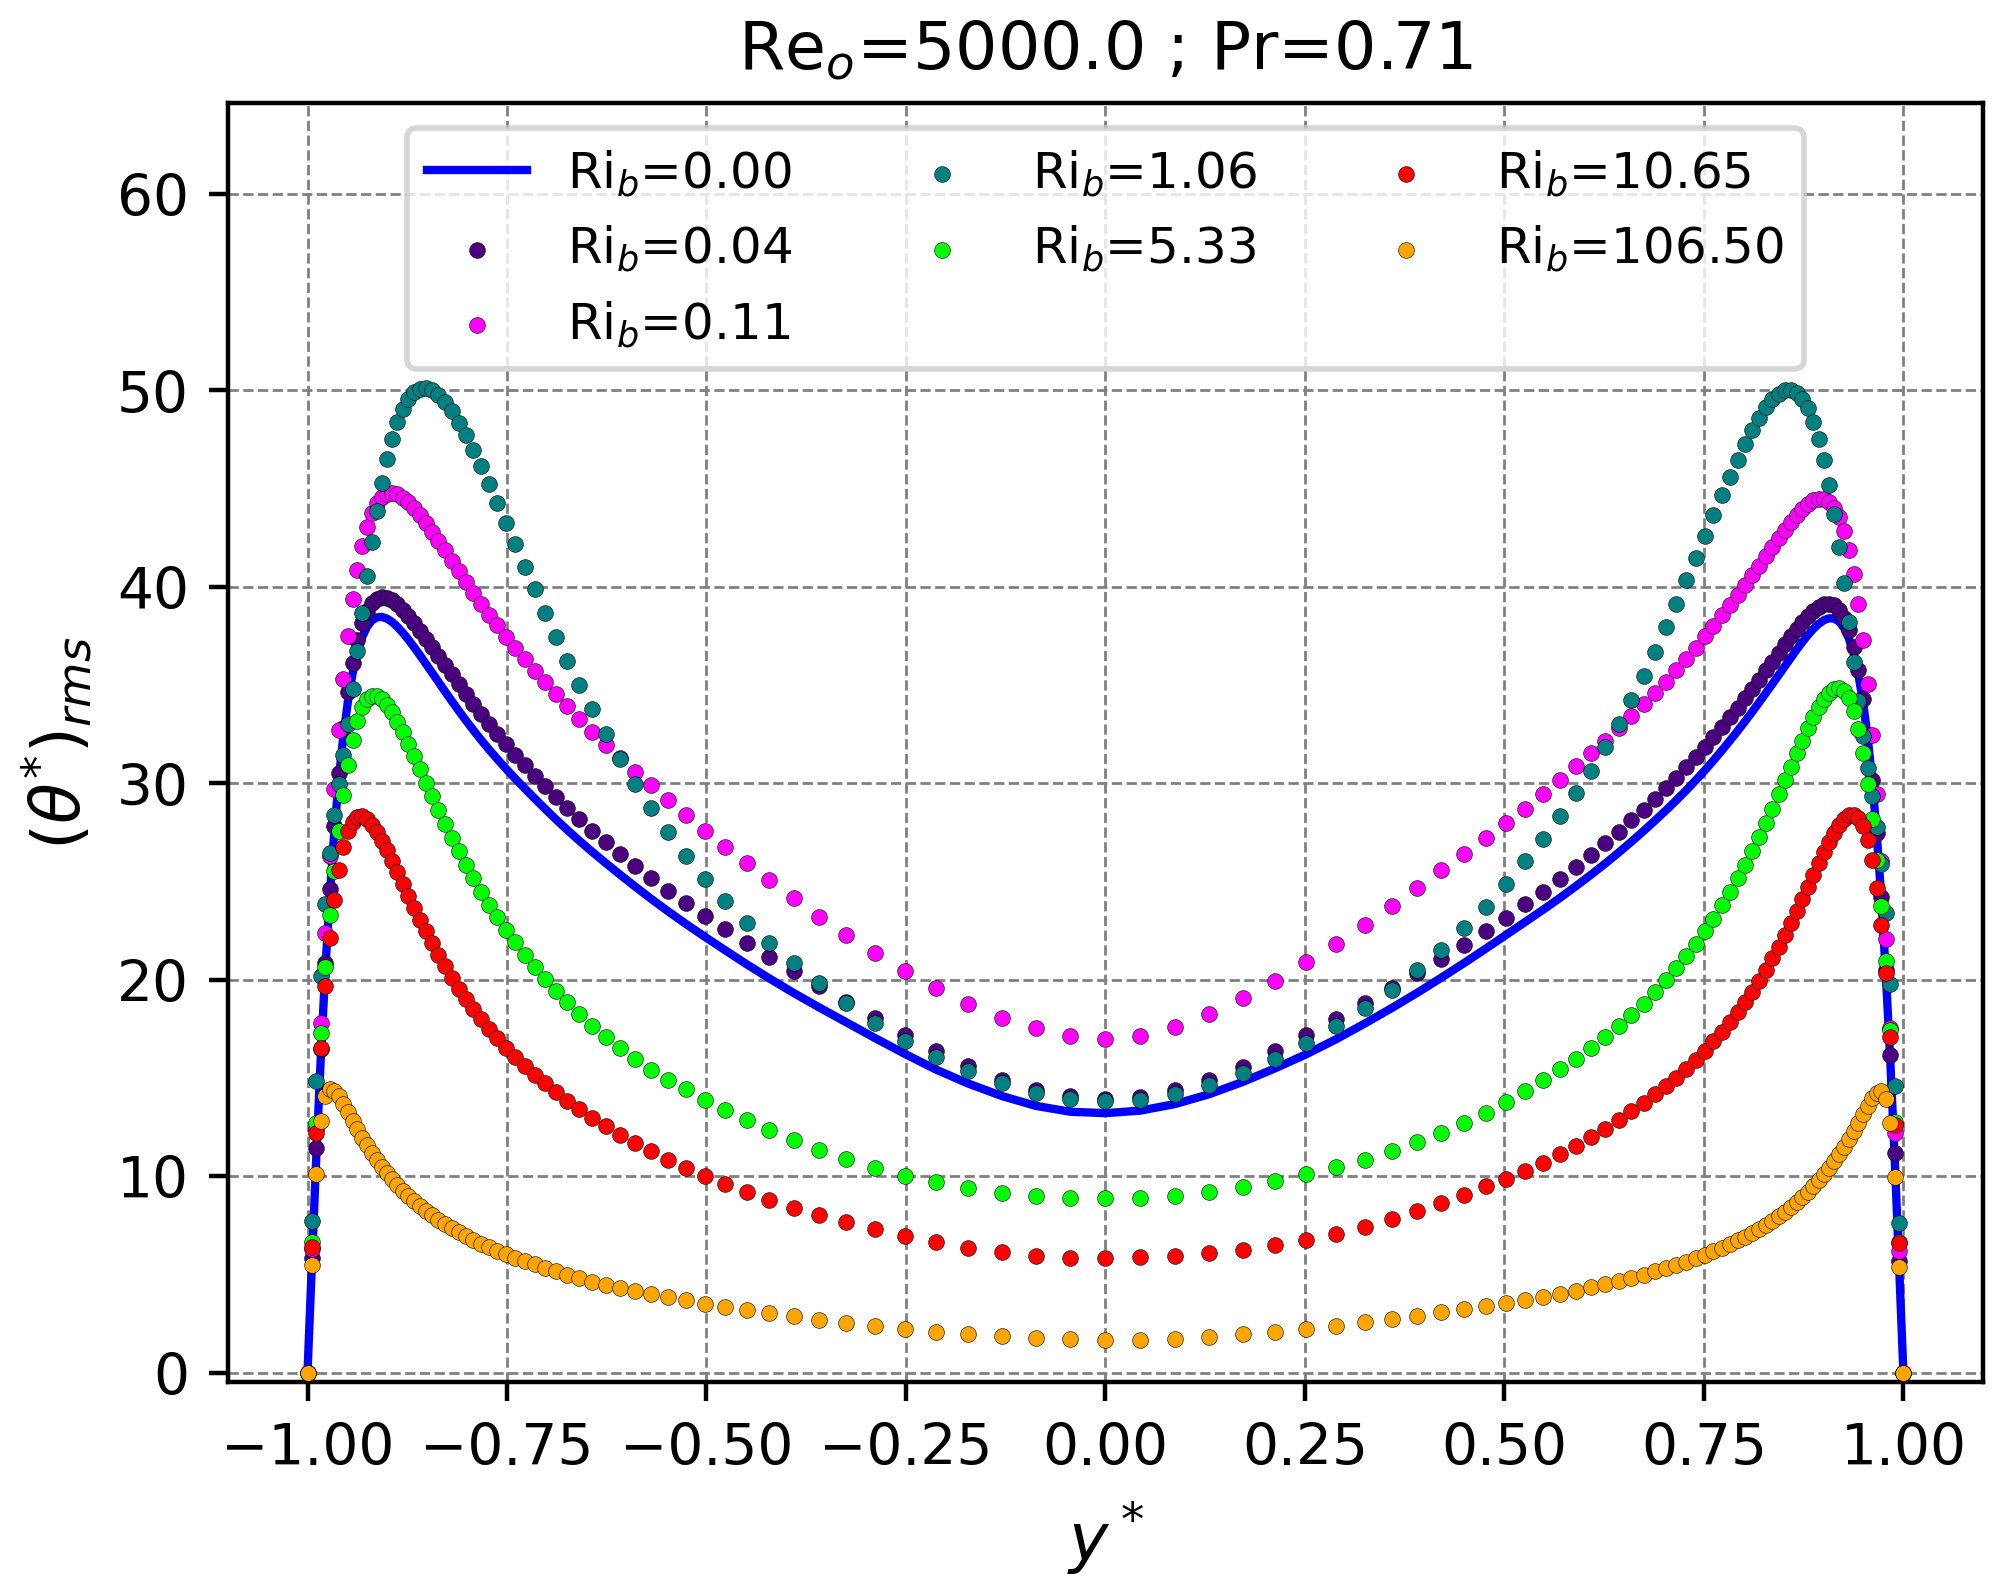
\includegraphics[width=0.49\textwidth]{figures/cap5/Re5000-Pr071/phi_rms_profile.png}
    	\label{fig:rms-phi-log-Re5000-Pr071}}
  \subfloat[]{
    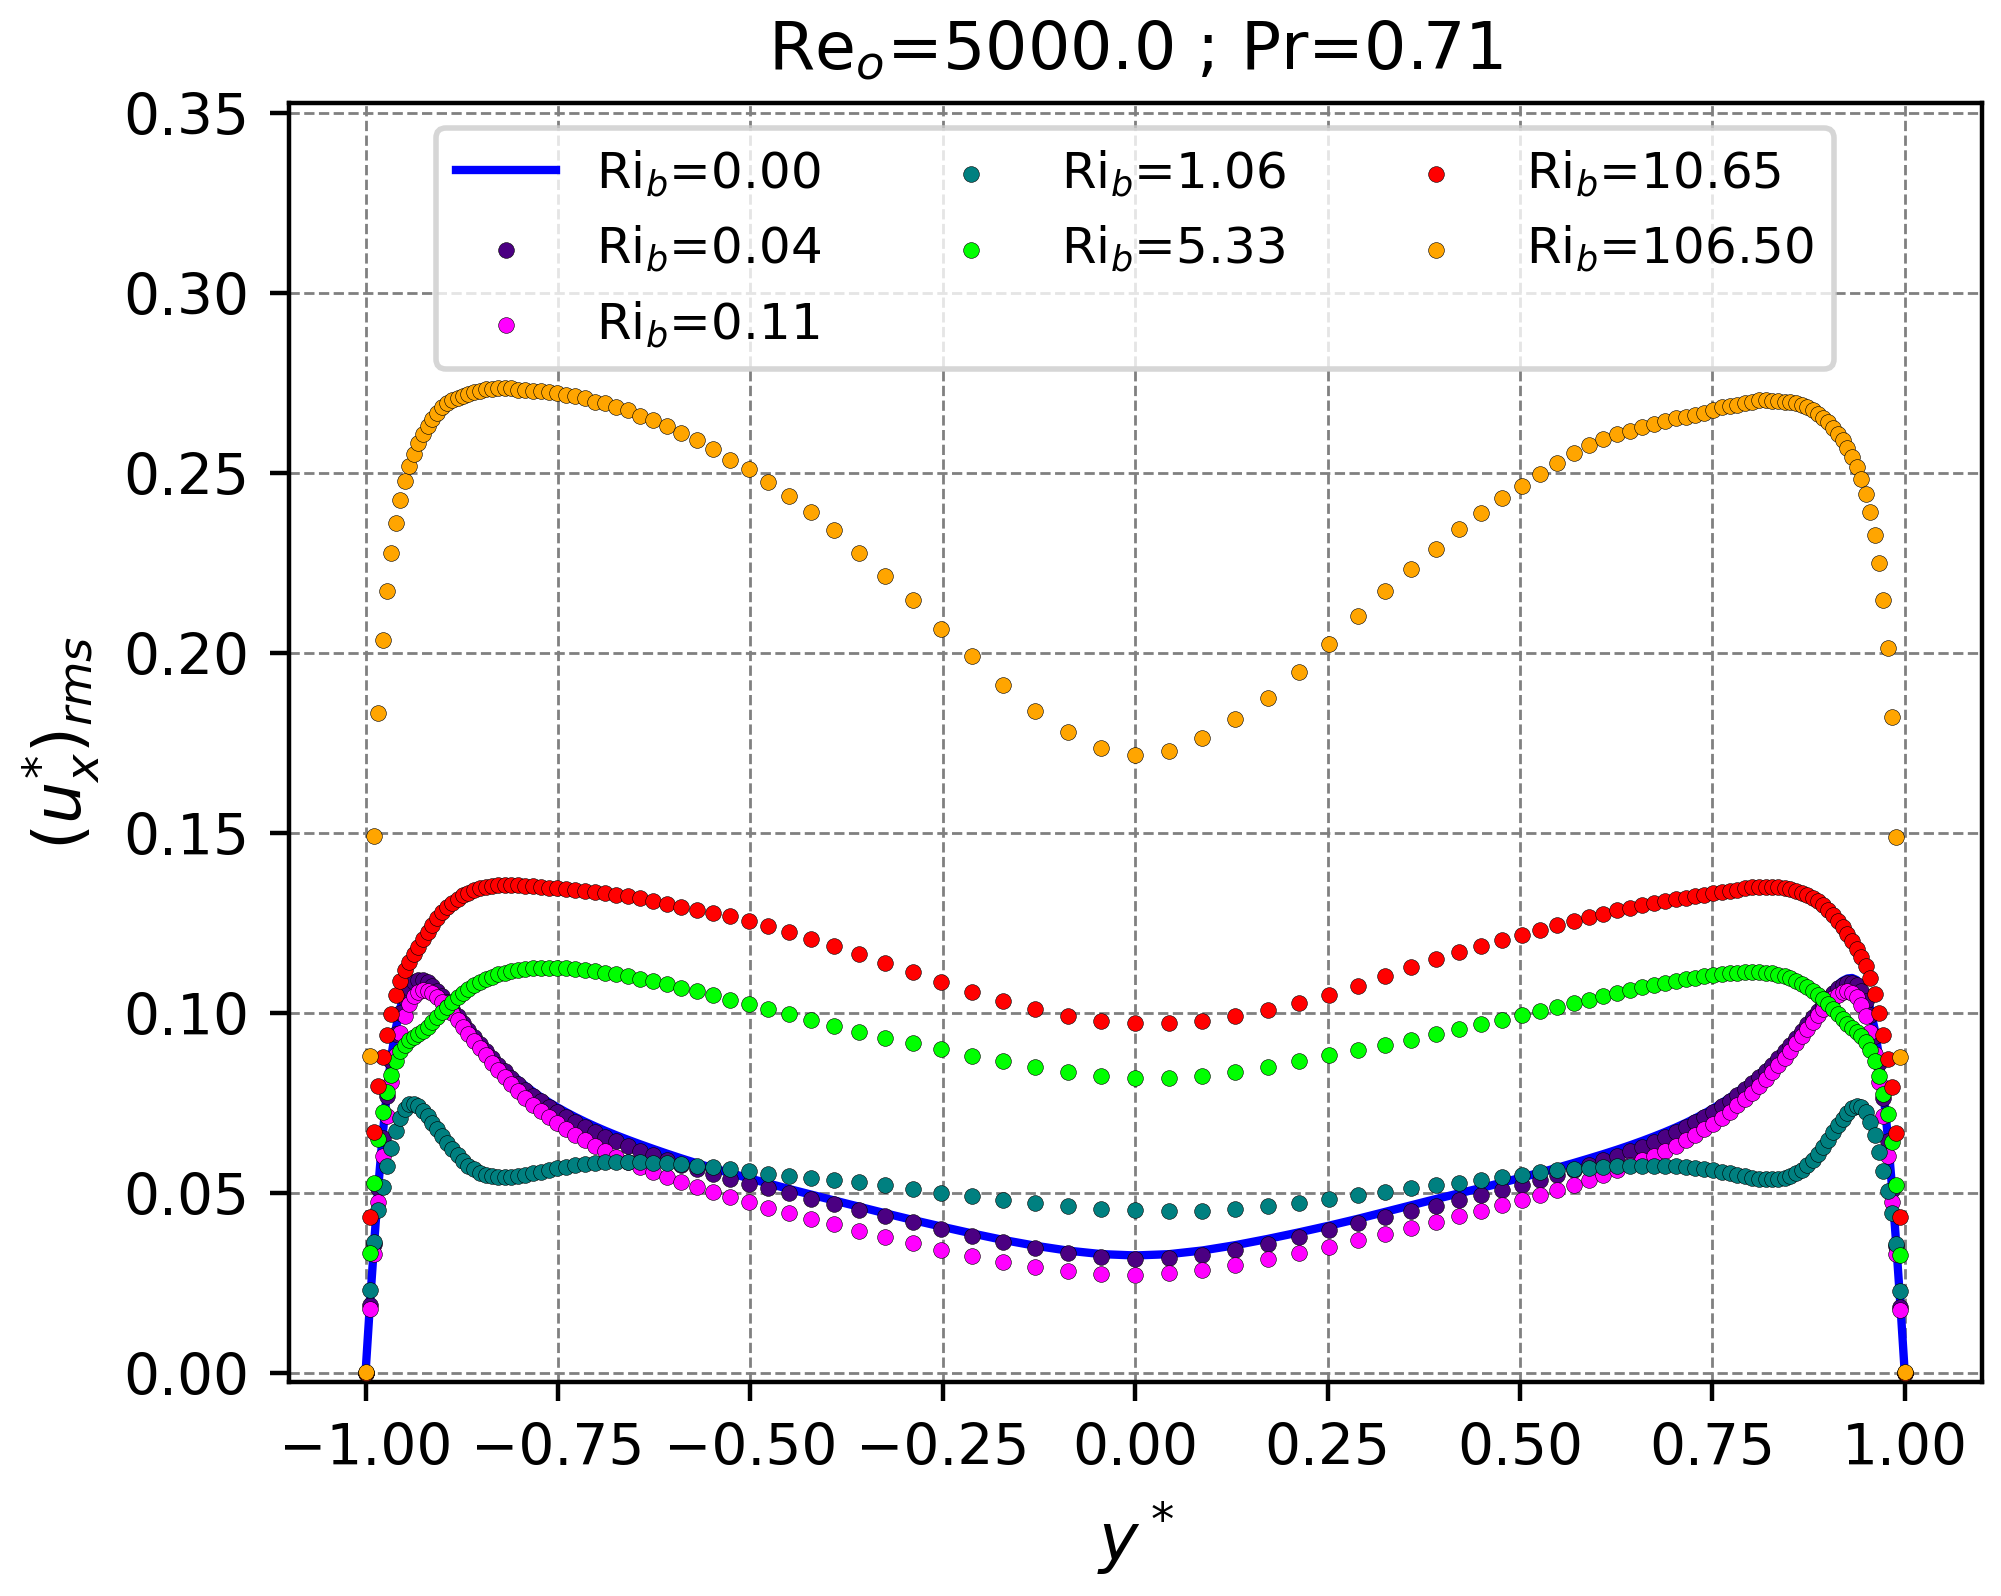
\includegraphics[width=0.49\textwidth]{figures/cap5/Re5000-Pr071/ux_rms_profile.png}
    	\label{fig:rms-ux-Re5000-Pr071}}
    \caption{Fluctuaciones RMS: \textbf{(a)} la boyancia atenúa $\theta^*_{\text{rms}}$ y \textbf{(b)}, eleva $u^*_{\text{rms}}$, intensificando la turbulencia.}
\end{figure}

La Figura \ref{fig:uxphi_f-Re5000-Pr071} muestra el perfil de la correlación $\langle u_x^{*'} \theta^{*'} \rangle$. Dado que el flujo de calor convectivo obedece, en primer orden, a $q'' \simeq \rho \hspace{0.5mm} c_P \hspace{0.5mm} U \hspace{0.5mm} \Delta T$, esta correlación puede interpretarse como proporcional al flujo de calor turbulento en la dirección $x$, es decir, al calor transportado por las estructuras turbulentas del flujo \cite{kundu, pope2001turbulent}. Para valores de Ri$_b$ próximos a cero (es decir, la convección forzada predomina), dichas estructuras trasportan el calor sobre todo en las proximidades de las paredes. Sin embargo, al aumentar la fuerza boyante, el signo de $\langle u_x^{*'} \theta^{*'} \rangle$ se invierte en la región central del canal: el flujo de calor turbulento se orienta contracorriente, de modo que regiones más frías de fluido son arrastradas aguas abajo. Este mecanismo disminuye la eficiencia global de la transferencia de calor.

Los cambios descritos en las fluctuaciones de temperatura y en el flujo turbulento $\langle u_x'\theta'\rangle$ repercuten directamente en la transferencia global de calor. En particular, la reducción de este flujo en el núcleo del canal para Bo$\lesssim3\times10^{-5}$ anticipa la caída del número de Nusselt, mientras que su posterior aumento (resultado de la mezcla intensificada por la fuerza boyante) explica la recuperación de $Nu$ a valores superiores al caso puramente forzado.

\begin{figure}[H]
\centering
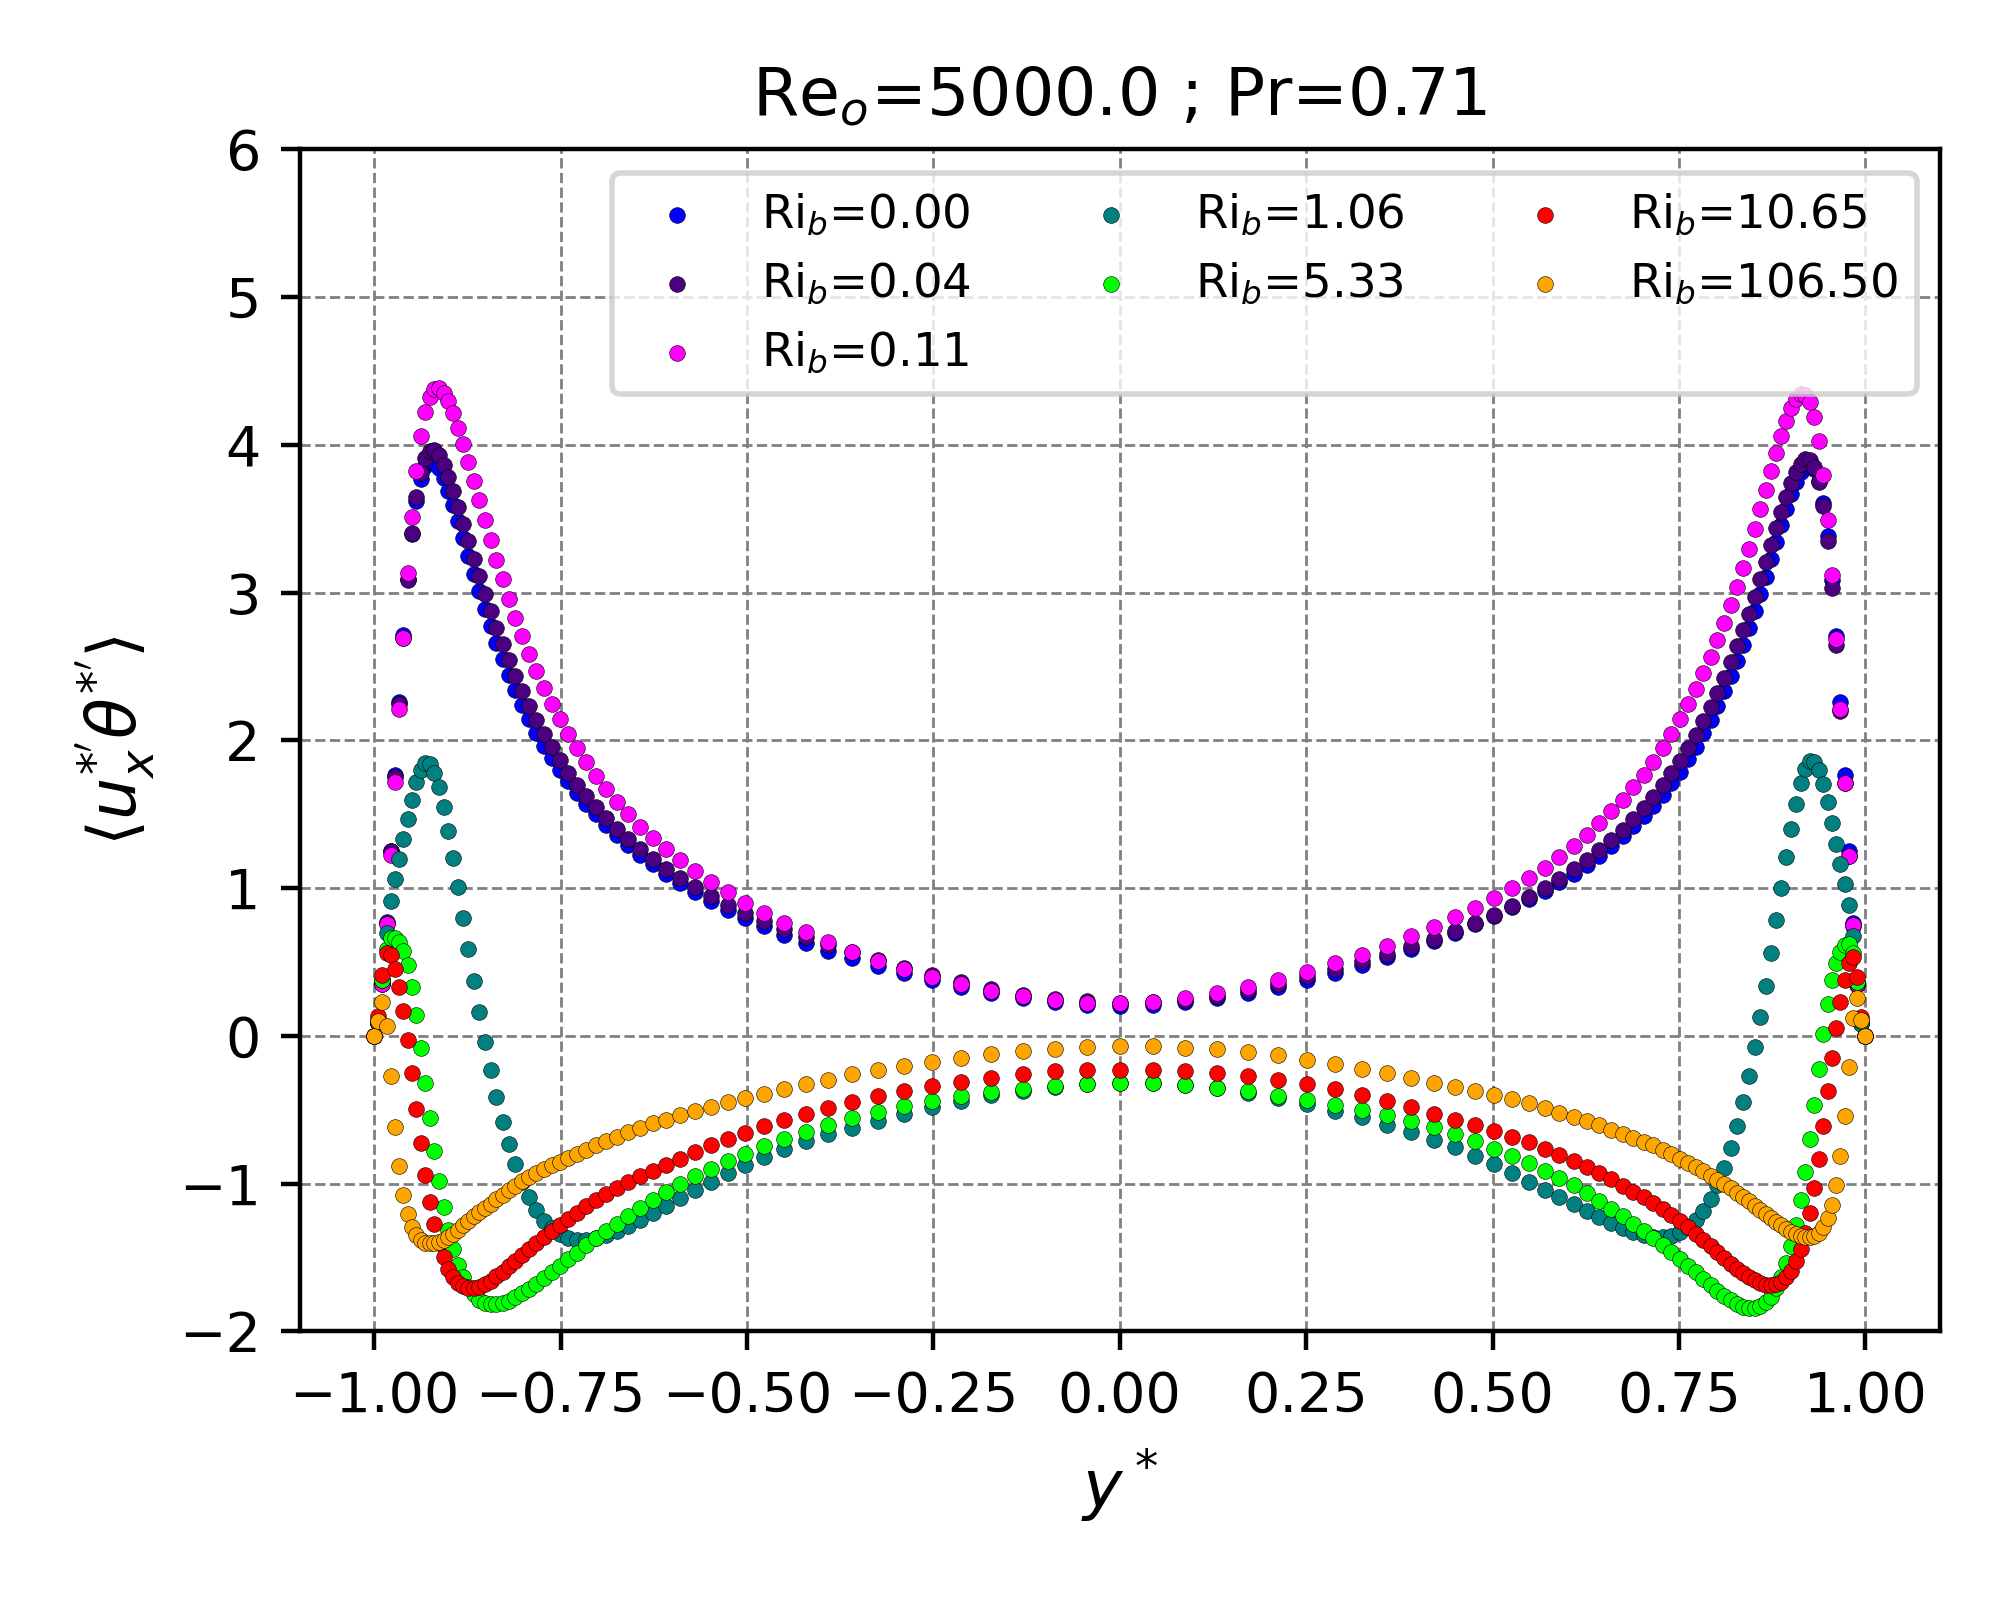
\includegraphics[width=0.6\textwidth]{figures/cap5/Re5000-Pr071/uphif_profile.png}
\caption{Flujo de calor turbulento \textit{streamwise} $\langle u^{*'}_x \theta^{*'} \rangle$: a Ri$_b$ altos se invierte en el núcleo.}
\label{fig:uxphi_f-Re5000-Pr071}
\end{figure}


\section{Comparación entre casos de distinto Prandtl}

%En esta sección se compara los casos con Re$_o$=5000 y Pr=0.071,0.71. La Figura \ref{fig:plus-ux-Re5000-Prs} presenta lo perfiles de velocidad media en términos de \textit{wall units}. En la subcapa viscosa ($y^+ < 5$), es posible aproximar la velocidad como $\langle u_x^+ \rangle \simeq y^+ + \mathcal{O}((y^+)^2)$ \cite{pope2001turbulent}, cuya dicha aproximación está representada con la linea negra del gráfico. En esta región, el tensor de esfuerzo de Reynolds es despreciable comparado con el tensor de esfuerzo viscoso. En efecto, se puede apreciar que independientemente de la sustancia y de fuerza boyante, todos los casos muestran ser consistentes con dicha aproximación.

En esta sección se comparan los casos con $Re_o$ = 5000 y Pr = 0.071 y 0.71. La Figura \ref{fig:plus-ux-Re5000-Prs} muestra los perfiles de velocidad media expresados en unidades de pared (\textit{wall units}). En la subcapa viscosa ($y^+ < 5$) la velocidad puede aproximarse por
$$\langle u_x^+ \rangle \;\simeq\; y^+ + \mathcal{O} \left[(y^+)^{2} \right],$$
según Pope \cite{pope2001turbulent}. Esta ley se indica en la figura con la línea negra de referencia. En dicha región las tensiones de Reynolds son despreciables frente a las tensiones viscosas, de modo que el perfil depende casi exclusivamente de la distancia normalizada a la pared. Como puede verse, todos los casos, independientemente del número de Prandtl y de la fuerza boyante, siguen de cerca esta aproximación lineal, lo que confirma la validez de la ley en la subcapa viscosa. 

Por otra parte, en la región logarítmica (\textit{log-law region}), en condiciones de convección forzada, la velocidad media en la dirección de la corriente se alinea perfectamente con la ley logarítmica clásica \cite{kawamura2000dns}. Sin embargo, esta ley ya no es válida al considerar la flotabilidad \cite{zhou2024direct}. 

\begin{figure}[H]
  \centering
    \subfloat[]{
    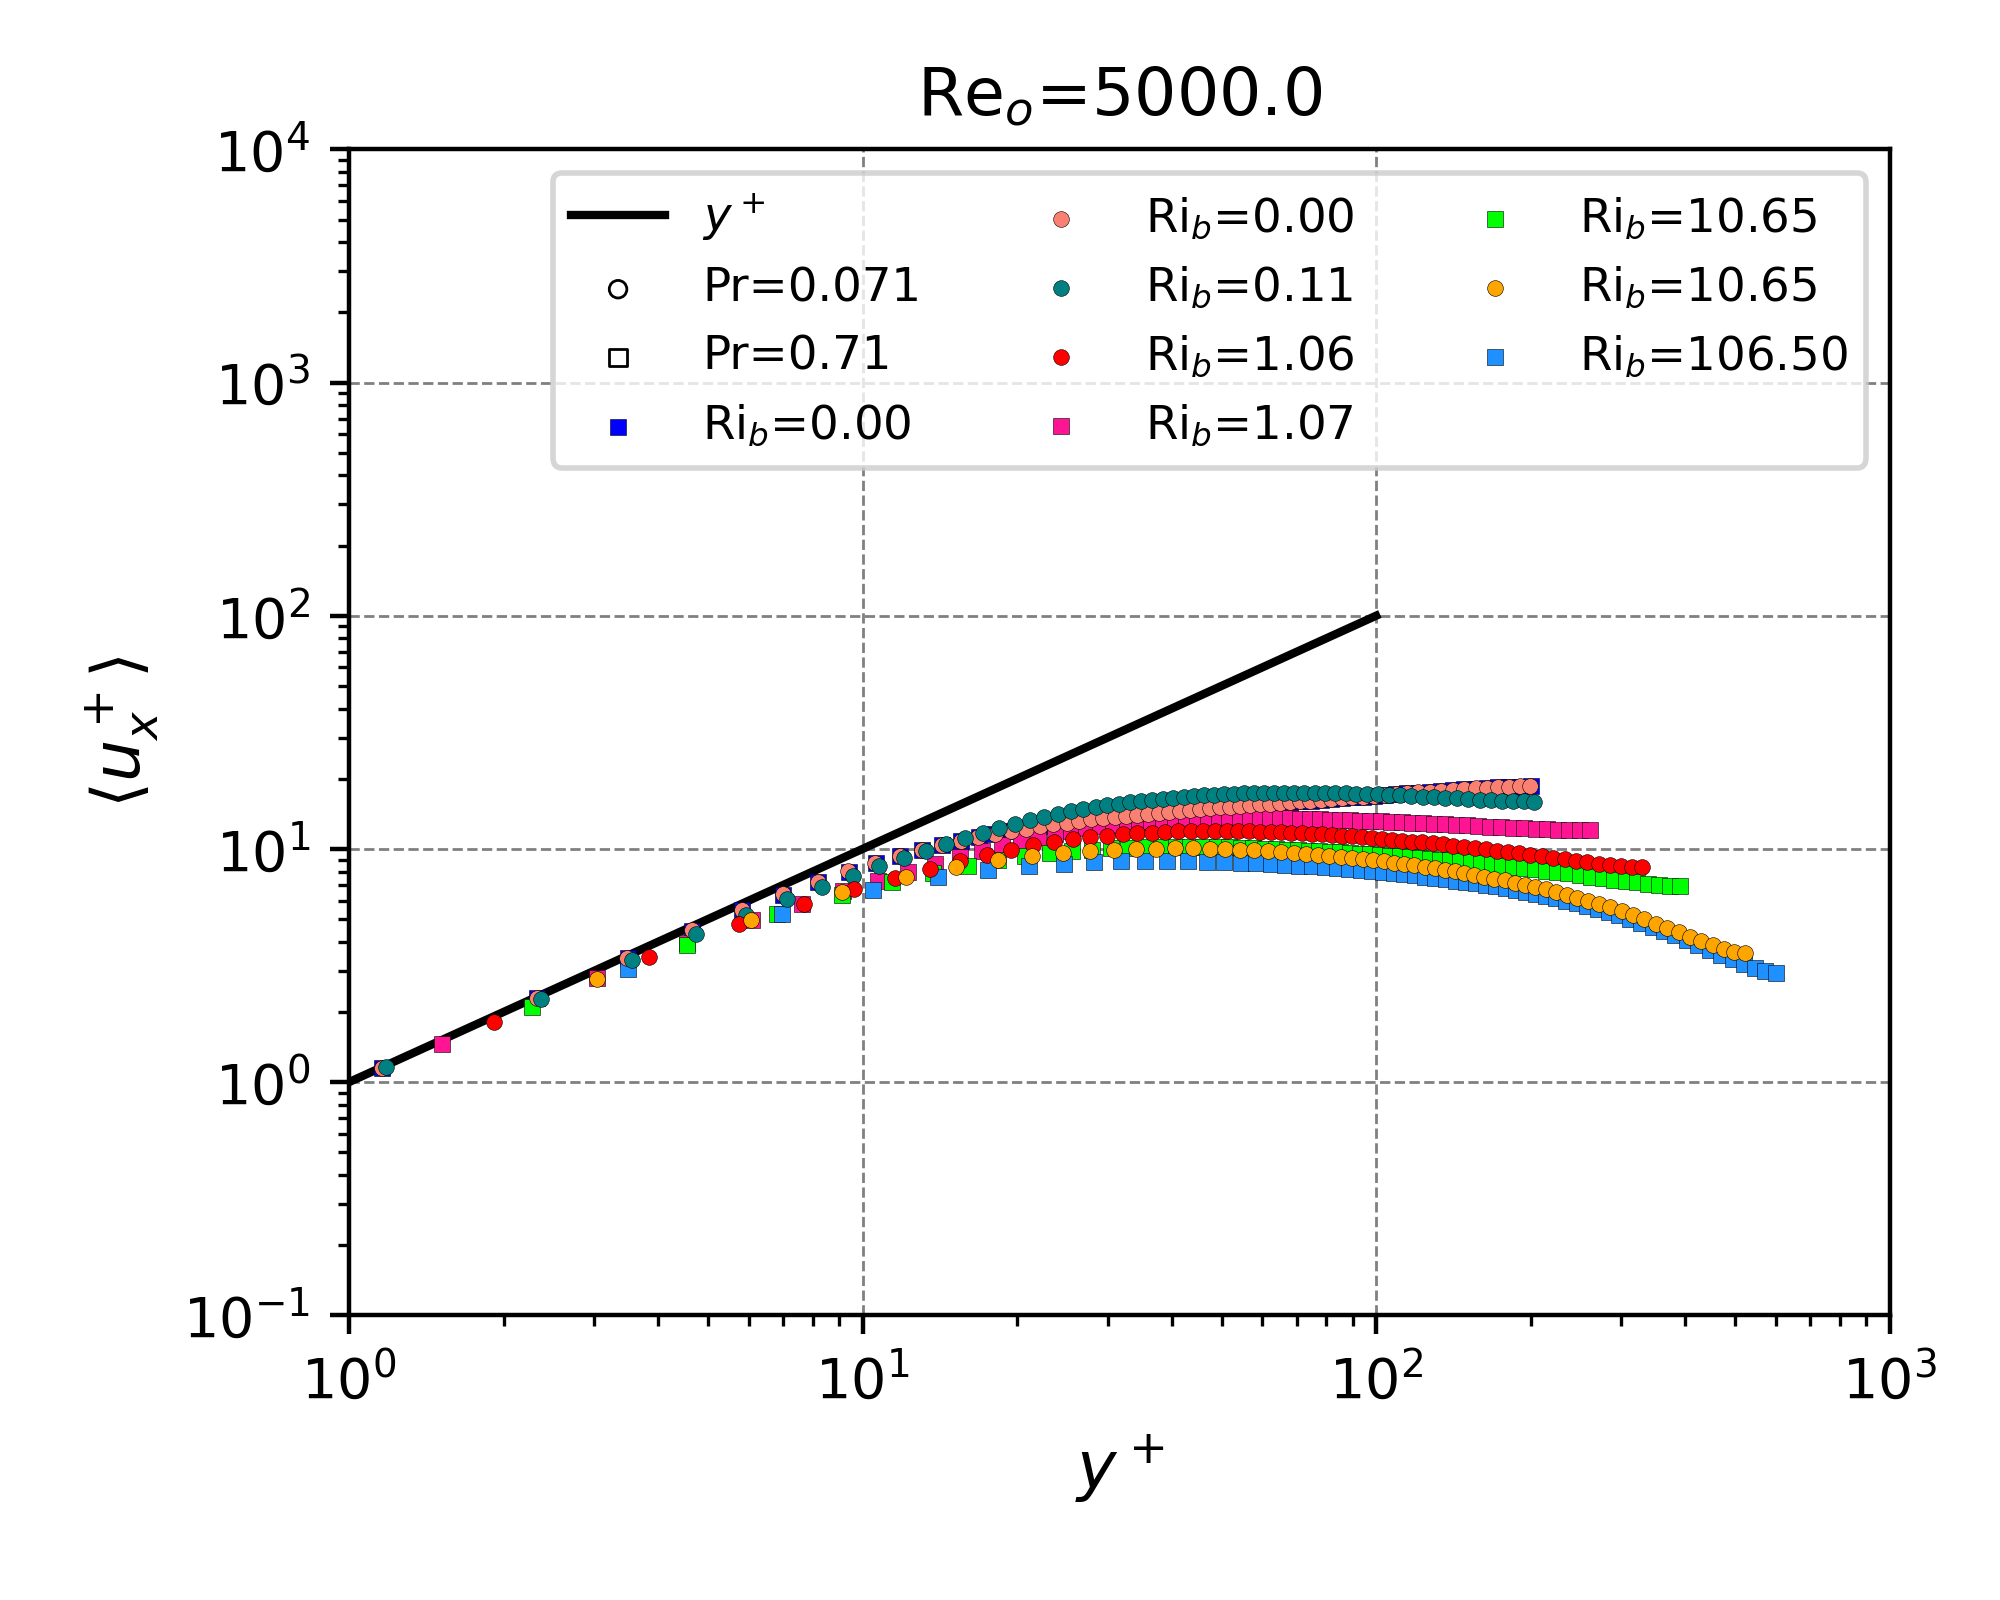
\includegraphics[width=0.5\textwidth]{figures/cap5/ux_mean_plus_log_profile.png}
  	  	\label{fig:plus-ux-Re5000-Prs}}
 	 \subfloat[]{
    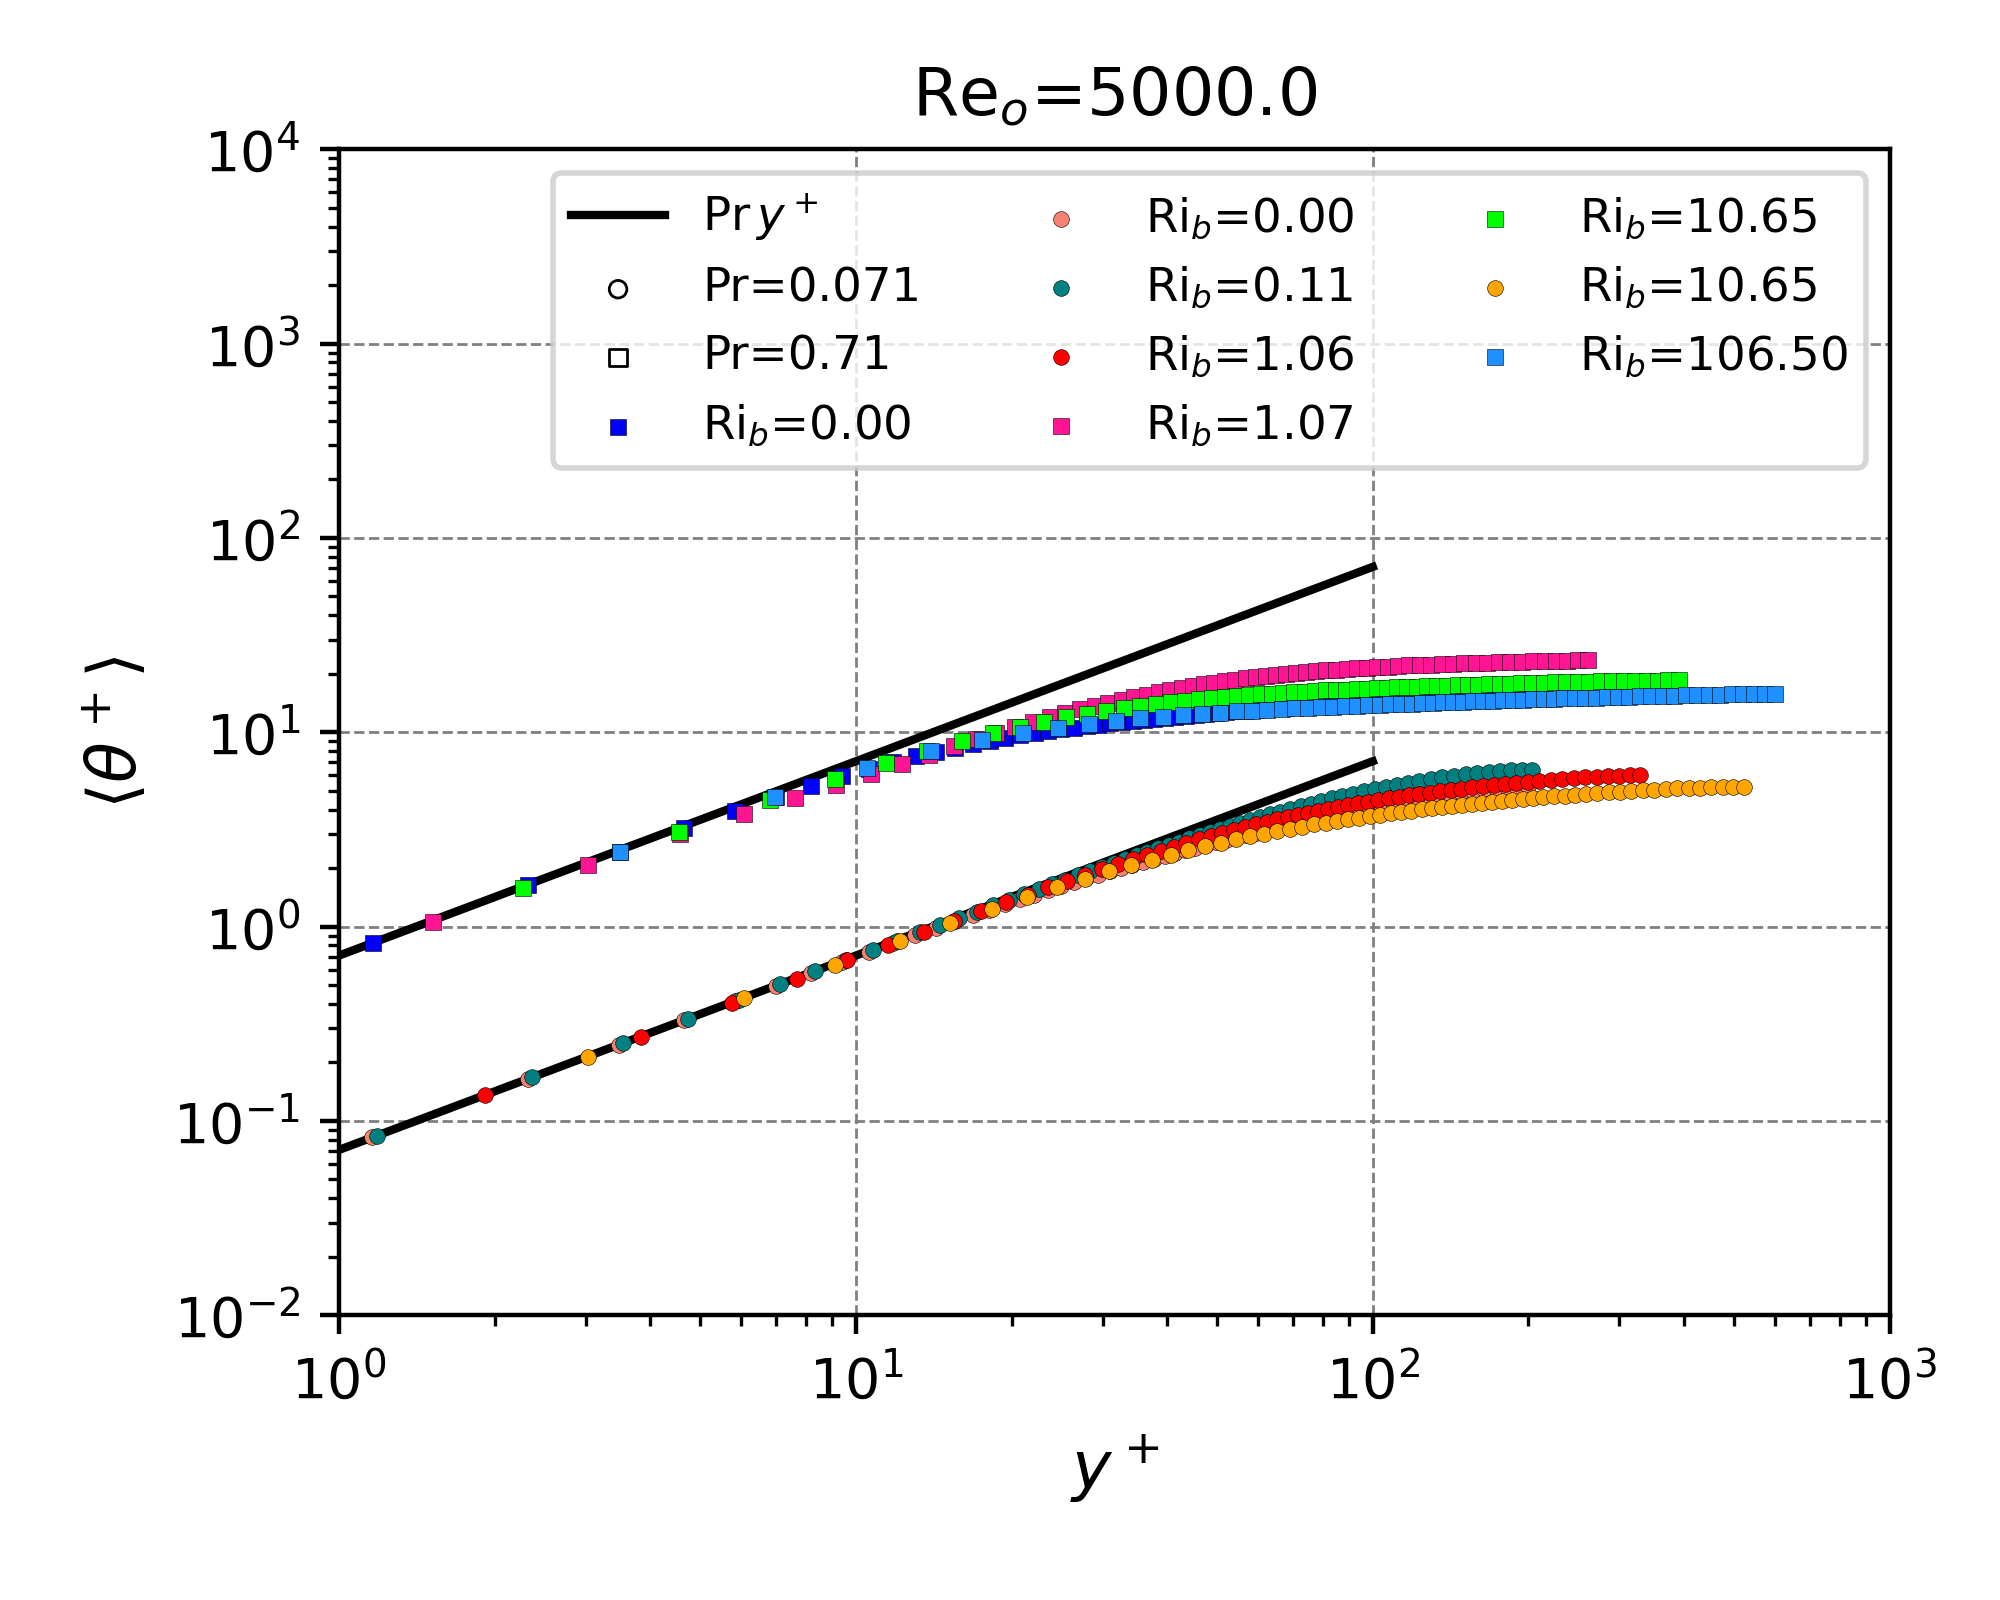
\includegraphics[width=0.5\textwidth]{figures/cap5/phi_mean_plus_log_profile.png}
    	\label{fig:plus-phi-Re5000-Prs}}
  \caption{Perfiles medios en unidades de pared para Re$_o$=5000 y Pr=0.071,0.71 y distintos valores de Ri$_b$.}
  \label{fig:Re5000-Pr071}
\end{figure}

%Por otra parte, en la Figura \ref{fig:plus-phi-Re5000-Prs} se presentan lo perfiles de temperatura media. Es posible aproximar la variación de la temperatura media cerca de la pared como proporcional a $y^+$ \cite{kawamura1998dns}:
%
%\begin{equation*}
%\langle \theta^* \rangle \simeq \text{Pr}\hspace{0.5mm} y^+
%\end{equation*}
% 
%Esta aproximación está representada en el gŕafico con lineas negras. Podemos ver que los casos con distinto Pr dicha aprox se corresponde con los datos de la simulación. Se aprecia que para el Pr más bajo la ley tiene un buen hasta $y^+ \sim 13$ mientras que para el más alto es menor, $y^+ \sim 7$. Esto está relacionado al hecho de que el fenómeno de conducción cerca la pared es más relevante que la convección para fluidos con difusividad térmica o Pr más bajos \cite{abregu2023dns}.



La Figura \ref{fig:plus-phi-Re5000-Prs} muestra los perfiles de temperatura adimensional media en unidades de pared. Cerca de la pared, la variación de la temperatura puede aproximarse por la relación lineal \cite{kawamura1998dns}
\begin{equation*}
\langle \theta^* \rangle \simeq \text{Pr}\hspace{0.5mm} y^+ ,
\end{equation*}
representada en la figura con líneas negras. Los resultados confirman esta ley para ambos números de Prandtl, aunque con distintos alcances: para el caso de Pr=0.071 la validez se extiende hasta $y^{+}\approx 30$, en concordancia con el trabajo de Zhou et al. \cite{zhou2024direct}. Sin embargo, para Pr=0.71 se reduce a $y^{+}\approx 7$. La diferencia se debe a que, en fluidos con menor difusividad térmica (Prandtl más bajo), el transporte de calor por conducción domina durante una mayor distancia normalizada desde la pared, retrasando la aparición del régimen convectivo predominante \cite{abregu2023dns}.






%\section{UHF vs UWT}
%
%En la sección [REF-VALIDACIONES] se utilizaron las simulaciones obtenidas por Guo y Prasser \cite{guo2022direct} para validar la herramienta numérica utilizada. El sistema estudiado por dichos autores corresponde a una configuración física distinta que al sistema estudiado en este trabajo, sin embargo, resulta útil comparar los perfiles de velocidad y temperatura, para entender en mayor profundidad el fenómeno de convección. En esta sección se pretende cotejar las dos configuraciones físicas establecidas: UHF\footnote{\textit{Uniform Heat Flux}} y UWT\footnote{\textit{Uniform Wall Temperature}}. El primero corresponde a los parámetros Re$_o$=3150, Pr=0.071 y Ri$_b$=0.67, y el segundo, a Re$_o$=3500, Pr=0.025 y Ri$_b$=0.5. Si bien los parámetros involucrados no son idénticos, están en el mismo orden de magnitud, para fines cualitativos, esto es más que adecuado para análizar la física detrás de ellos. Las Figuras \ref{fig:guocomp_ux} y \ref{fig:guocomp_phi} exponen los perfiles de velocidad en la dirección de la corriente y la temperatura de ambas configuraciones, respectivamente. En ambos casos se normaliza los perfiles con el máximo de la propia curva.  
%
%\begin{figure}[H]
%  \centering
%  \subfloat[]{
%    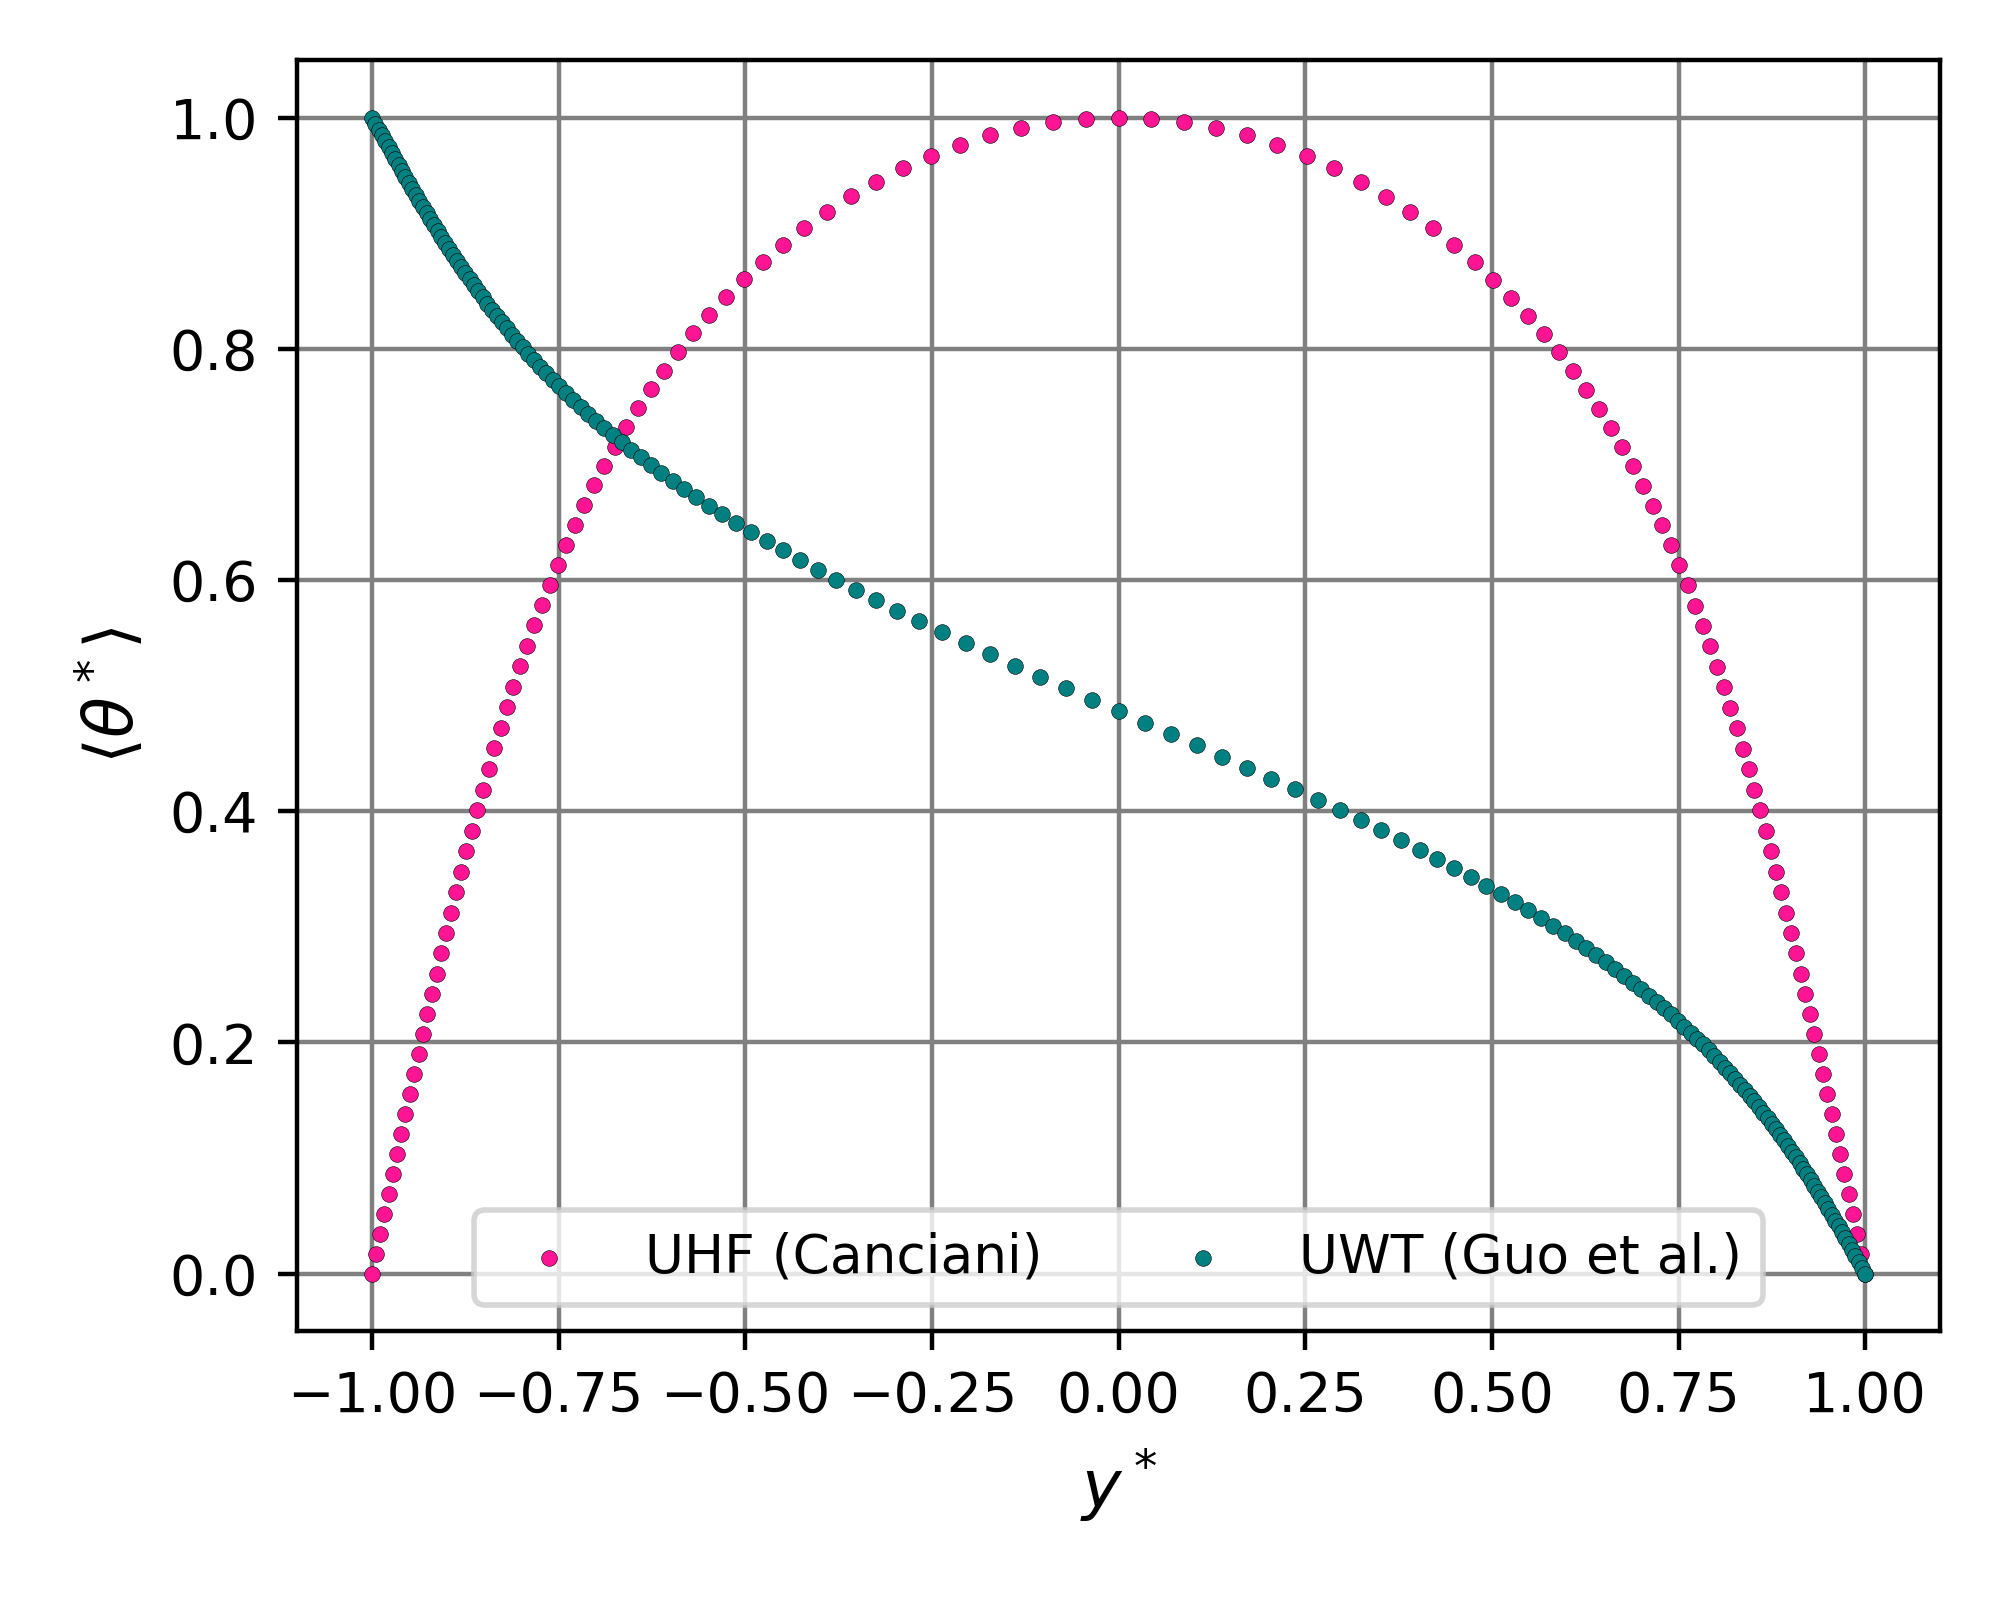
\includegraphics[width=0.49\textwidth]{figures/cap5/phi_mean_profile.png}
%    	\label{fig:guocomp_ux}}
%  \subfloat[]{
%    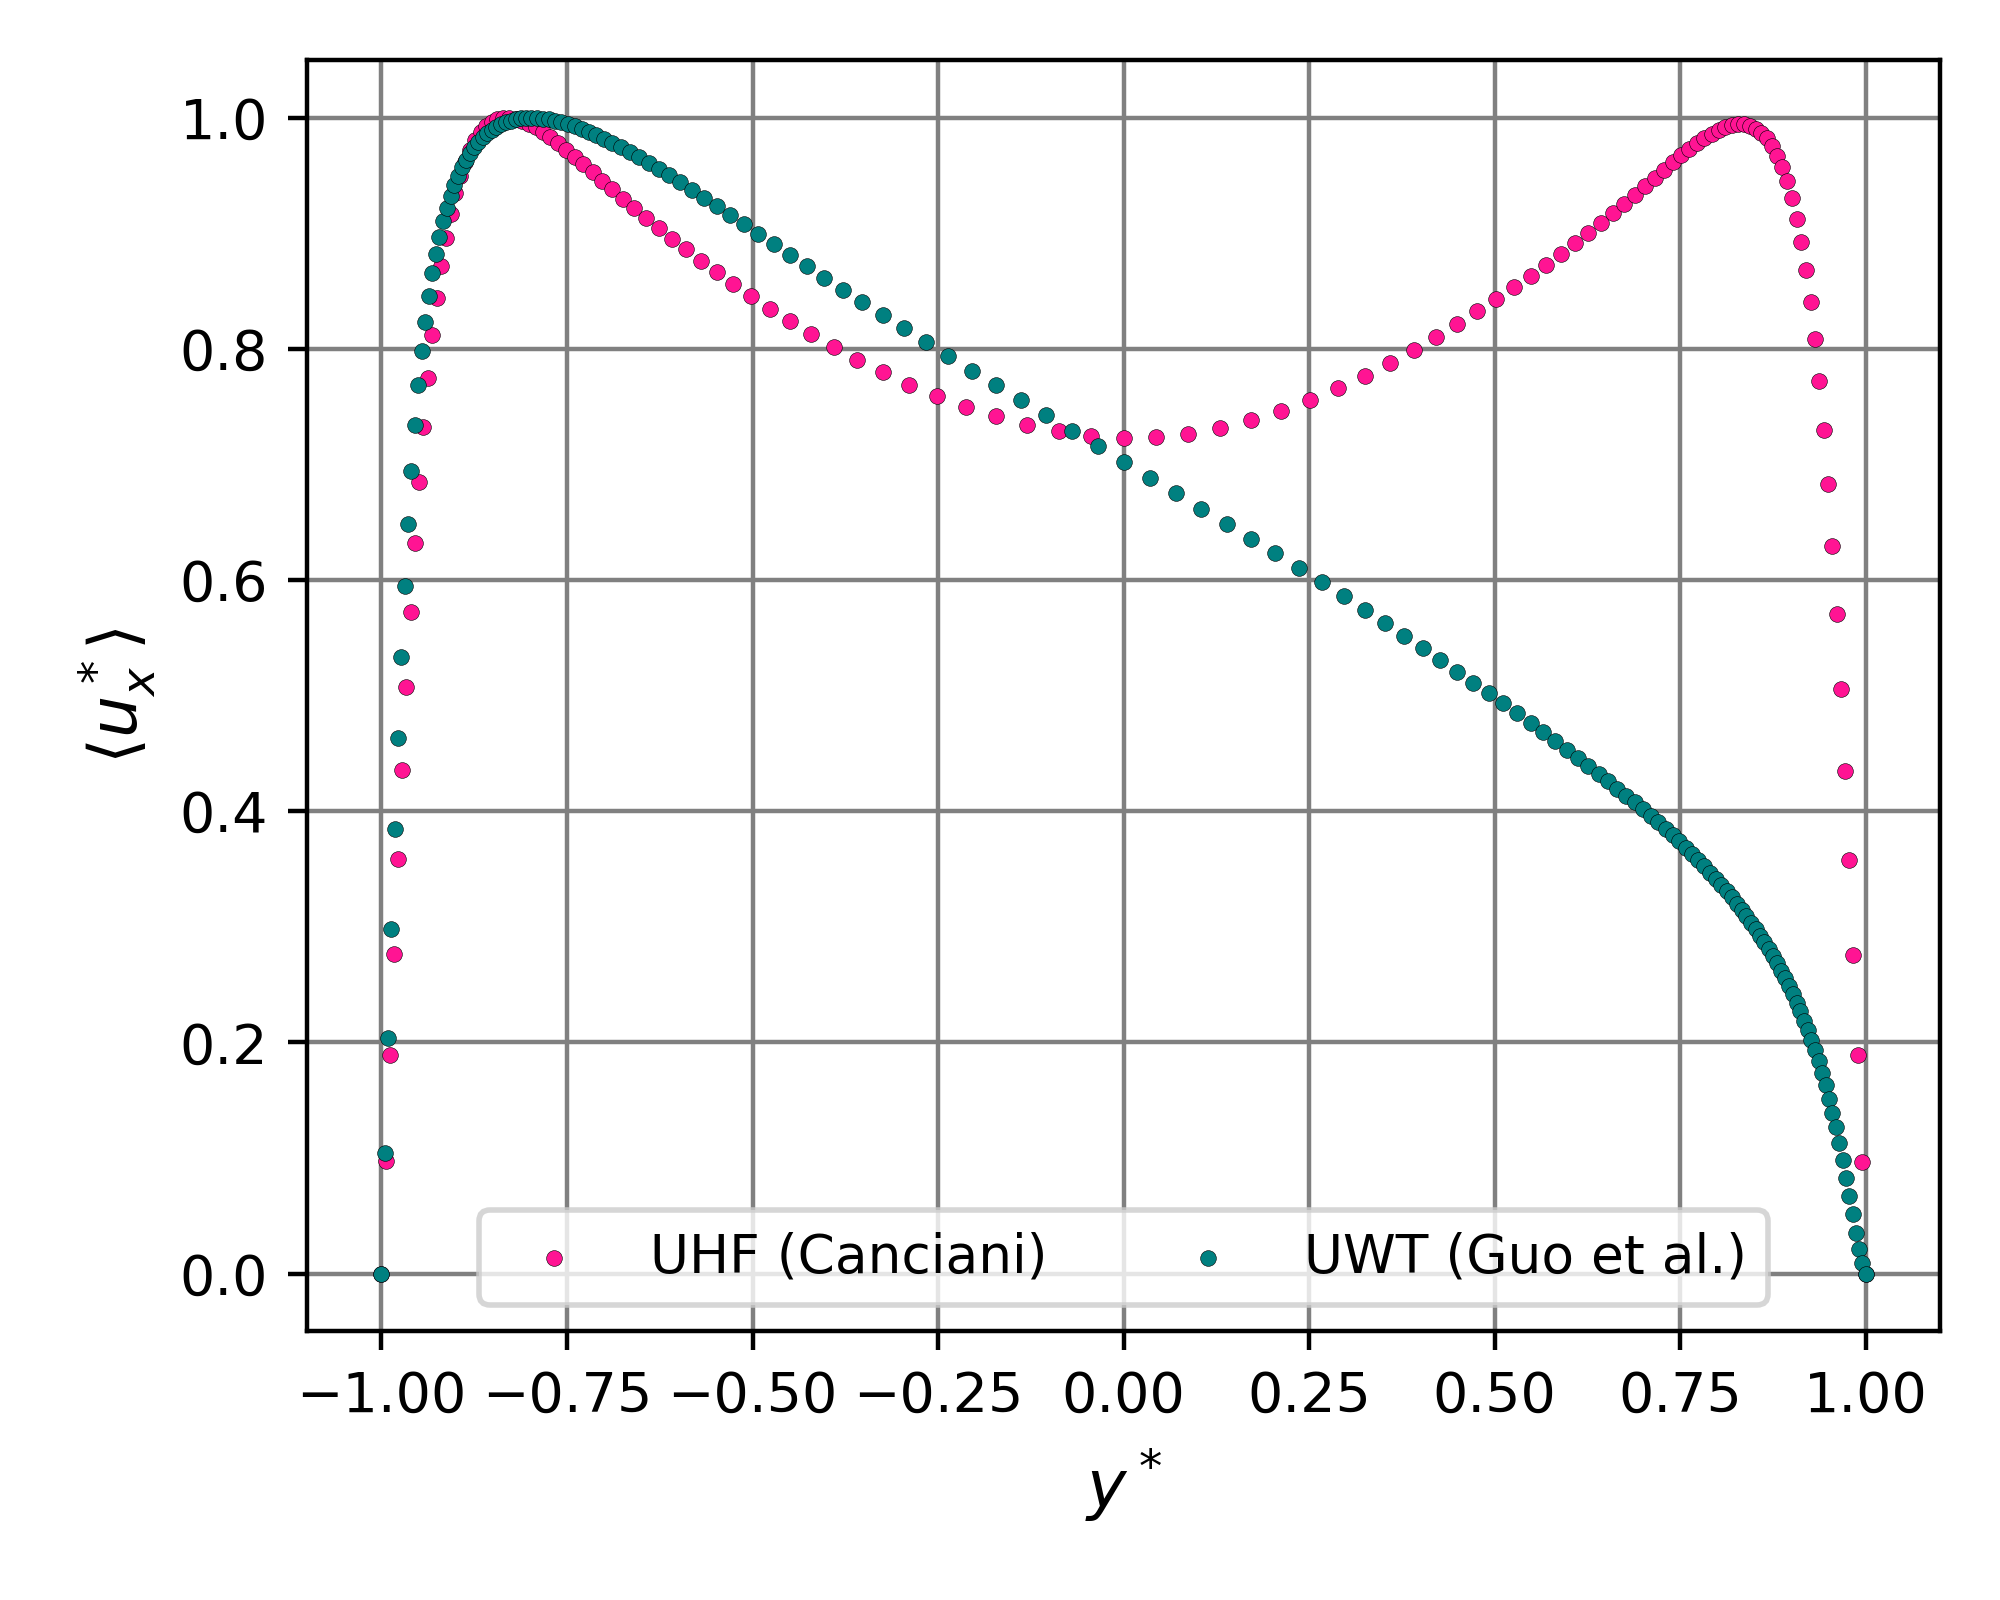
\includegraphics[width=0.49\textwidth]{figures/cap5/ux_mean_profile.png}
%    	\label{fig:guocomp_phi}}
%  \caption{Comparación entre los dos problemas.}
%  \label{fig:ux-guocomp}
%\end{figure}
%
%
%Una característica inmediata que se observa recae en la asimetría del los perfiles del caso UWT en comparación con UHF, lo que resulta claro debido a la asimetría del primero con respecto al segundo caso. 
%
%
%\textcolor{magenta}{seguir explicando la fisica de ambos casos.}



%\newpage
%\section{Número de Nusselt} \label{sec:nu}
%
%Desde una perspectiva ingenieríl, un parámetro importante que da información sobre la eficiencia de la transferencia de calor es el número de Nusselt (Nu), el cuál se define en la ecuación \ref{eq:nu}, donde $\overline{\theta_b}$ es la temperatura en \textit{bulk}.
%
%Un parámetro importante desde una perspectiva ingenieríl es el número de Nusselt (Nu), el cuál se define en la ecuación \ref{eq:nu}, donde $\overline{\theta_b}$ es la temperatura en \textit{bulk} (ecuación \ref{eq:tita_bulk}).
%
%\begin{equation}
%\text{Nu} = \frac{h L}{k} = \frac{2d \hspace*{1mm} q''_w}{k \hspace*{1mm} \overline{\theta^*_b}} = \frac{4}{3} \frac{Re_o Pr}{\overline{\theta^*_b}}	
%\label{eq:nu}
%\end{equation}
%
%\begin{equation*}
%\overline{\theta_b} = \frac{\frac{1}{A} \int \langle u_x \theta \rangle }{U_b} = \frac{\int^d_0 \langle u_x \theta \rangle \hspace*{0.5mm} dy }{\int^d_0 \langle u_x \rangle \hspace*{0.5mm} dy}
%\label{eq:tita_bulk}
%\end{equation*}
%
%En la Figura \ref{fig:nu_vs_bo} se presentan todos los valores de Nu obtenidos, graficados en función del número de boyancia Bo, definido en la ecuación \ref{eq:jackson_bo}, el cuál da una idea del \textit{ratio} entre las intensidad de las fuerzas boyantes y el la fuerza impulsora de la convección forzada. Los valores se contrastan con la correlación de Jackson et al. \cite{jackson1989studies}, expresada en la ecuación \ref{eq:jackson_corr}. Los valores Nu están normalizados con el Nu de convección forzada puro Nu$_{fc}$ el cuál es obtenido a partir de la correlación de Dittus-Boelter \cite{incropera}. Además, se añaden otros valores de Nu obtenidos mediante simulaciones DNS \cite{you2003direct} a modo de comparativa y se puede observar que los mismos se alinean con la tendencia de la correlación al igual que nuestro caso. 
%
%En la Figura \ref{fig:parity} se muestra un gráfico de paridad entre los números de Nusselt obtenidos por DNS, $Nu_{\text{DNS}}/Nu_{DB}$ (eje $x$), y los calculados con la correlación de Jackson, $Nu_{\text{corr}}/Nu_{DB}$ (eje $y$). La línea negra representa el acuerdo perfecto ($y=x$), mientras que las líneas azules punteadas señalan la banda de $\pm2\sigma$ alrededor de esa bisectriz. Puede verse que prácticamente todos los puntos experimentales se agrupan muy cerca de la bisectriz y permanecen dentro de la banda de $\pm2\sigma$, evidenciando que la correlación de Jackson reproduce con buena precisión los valores simulados a lo largo de todo el rango de $Nu_{\text{DNS}}/Nu_{DB}$ considerado.
%
%
%Pueden distinguir 3 regiones principales
%\begin{itemize}
% \item[$\bullet$] para Bo $\lesssim$ $10^{-6}$ el valor Nu es practicamente igual a Nu$_{fc}$, es decir, domina la convección forzada,
% \item[$\bullet$] en el rango $10^{-6}$ $\lesssim$ Bo $\lesssim$ $3 \times 10^{-5}$ se observa una caida y una recuperación del número de Nusselt, revelando la existencia de una región donde la transferencia de calor empeora por debajo del caso únicamente forzada y que luego retoma su condición original,
% \item[$\bullet$] por último, para Bo $\gtrsim$ $3 \times 10^{-5}$ la transferencia de calor aumenta notoriamente, impulsado por las corrientes de convección natural que en esta región tiene mayor preponderancia.
%\end{itemize}
%
%%\vspace*{-1.5cm}
%
%\begin{equation}
%\text{Bo}= \frac{Gr*}{{\text{Re}_D}^{3.425} \hspace*{1mm} \text{Pr}^{0.8} }
%\label{eq:jackson_bo}
%\end{equation}
%
%\begin{equation}
%\frac{\text{Nu}}{\text{Nu}_{fc}}= \left\vert  1 - 8 \times 10^4 \hspace*{0.5mm} \text{Bo} \hspace*{0.5mm} \left( \frac{\text{Nu}}{\text{Nu}_{fc}} \right)^{-2}  \right\vert^{0.46}
%\label{eq:jackson_corr} 
%\end{equation}
%
%
%\begin{figure}[H]
%  \centering
%  \subfloat[]{
%    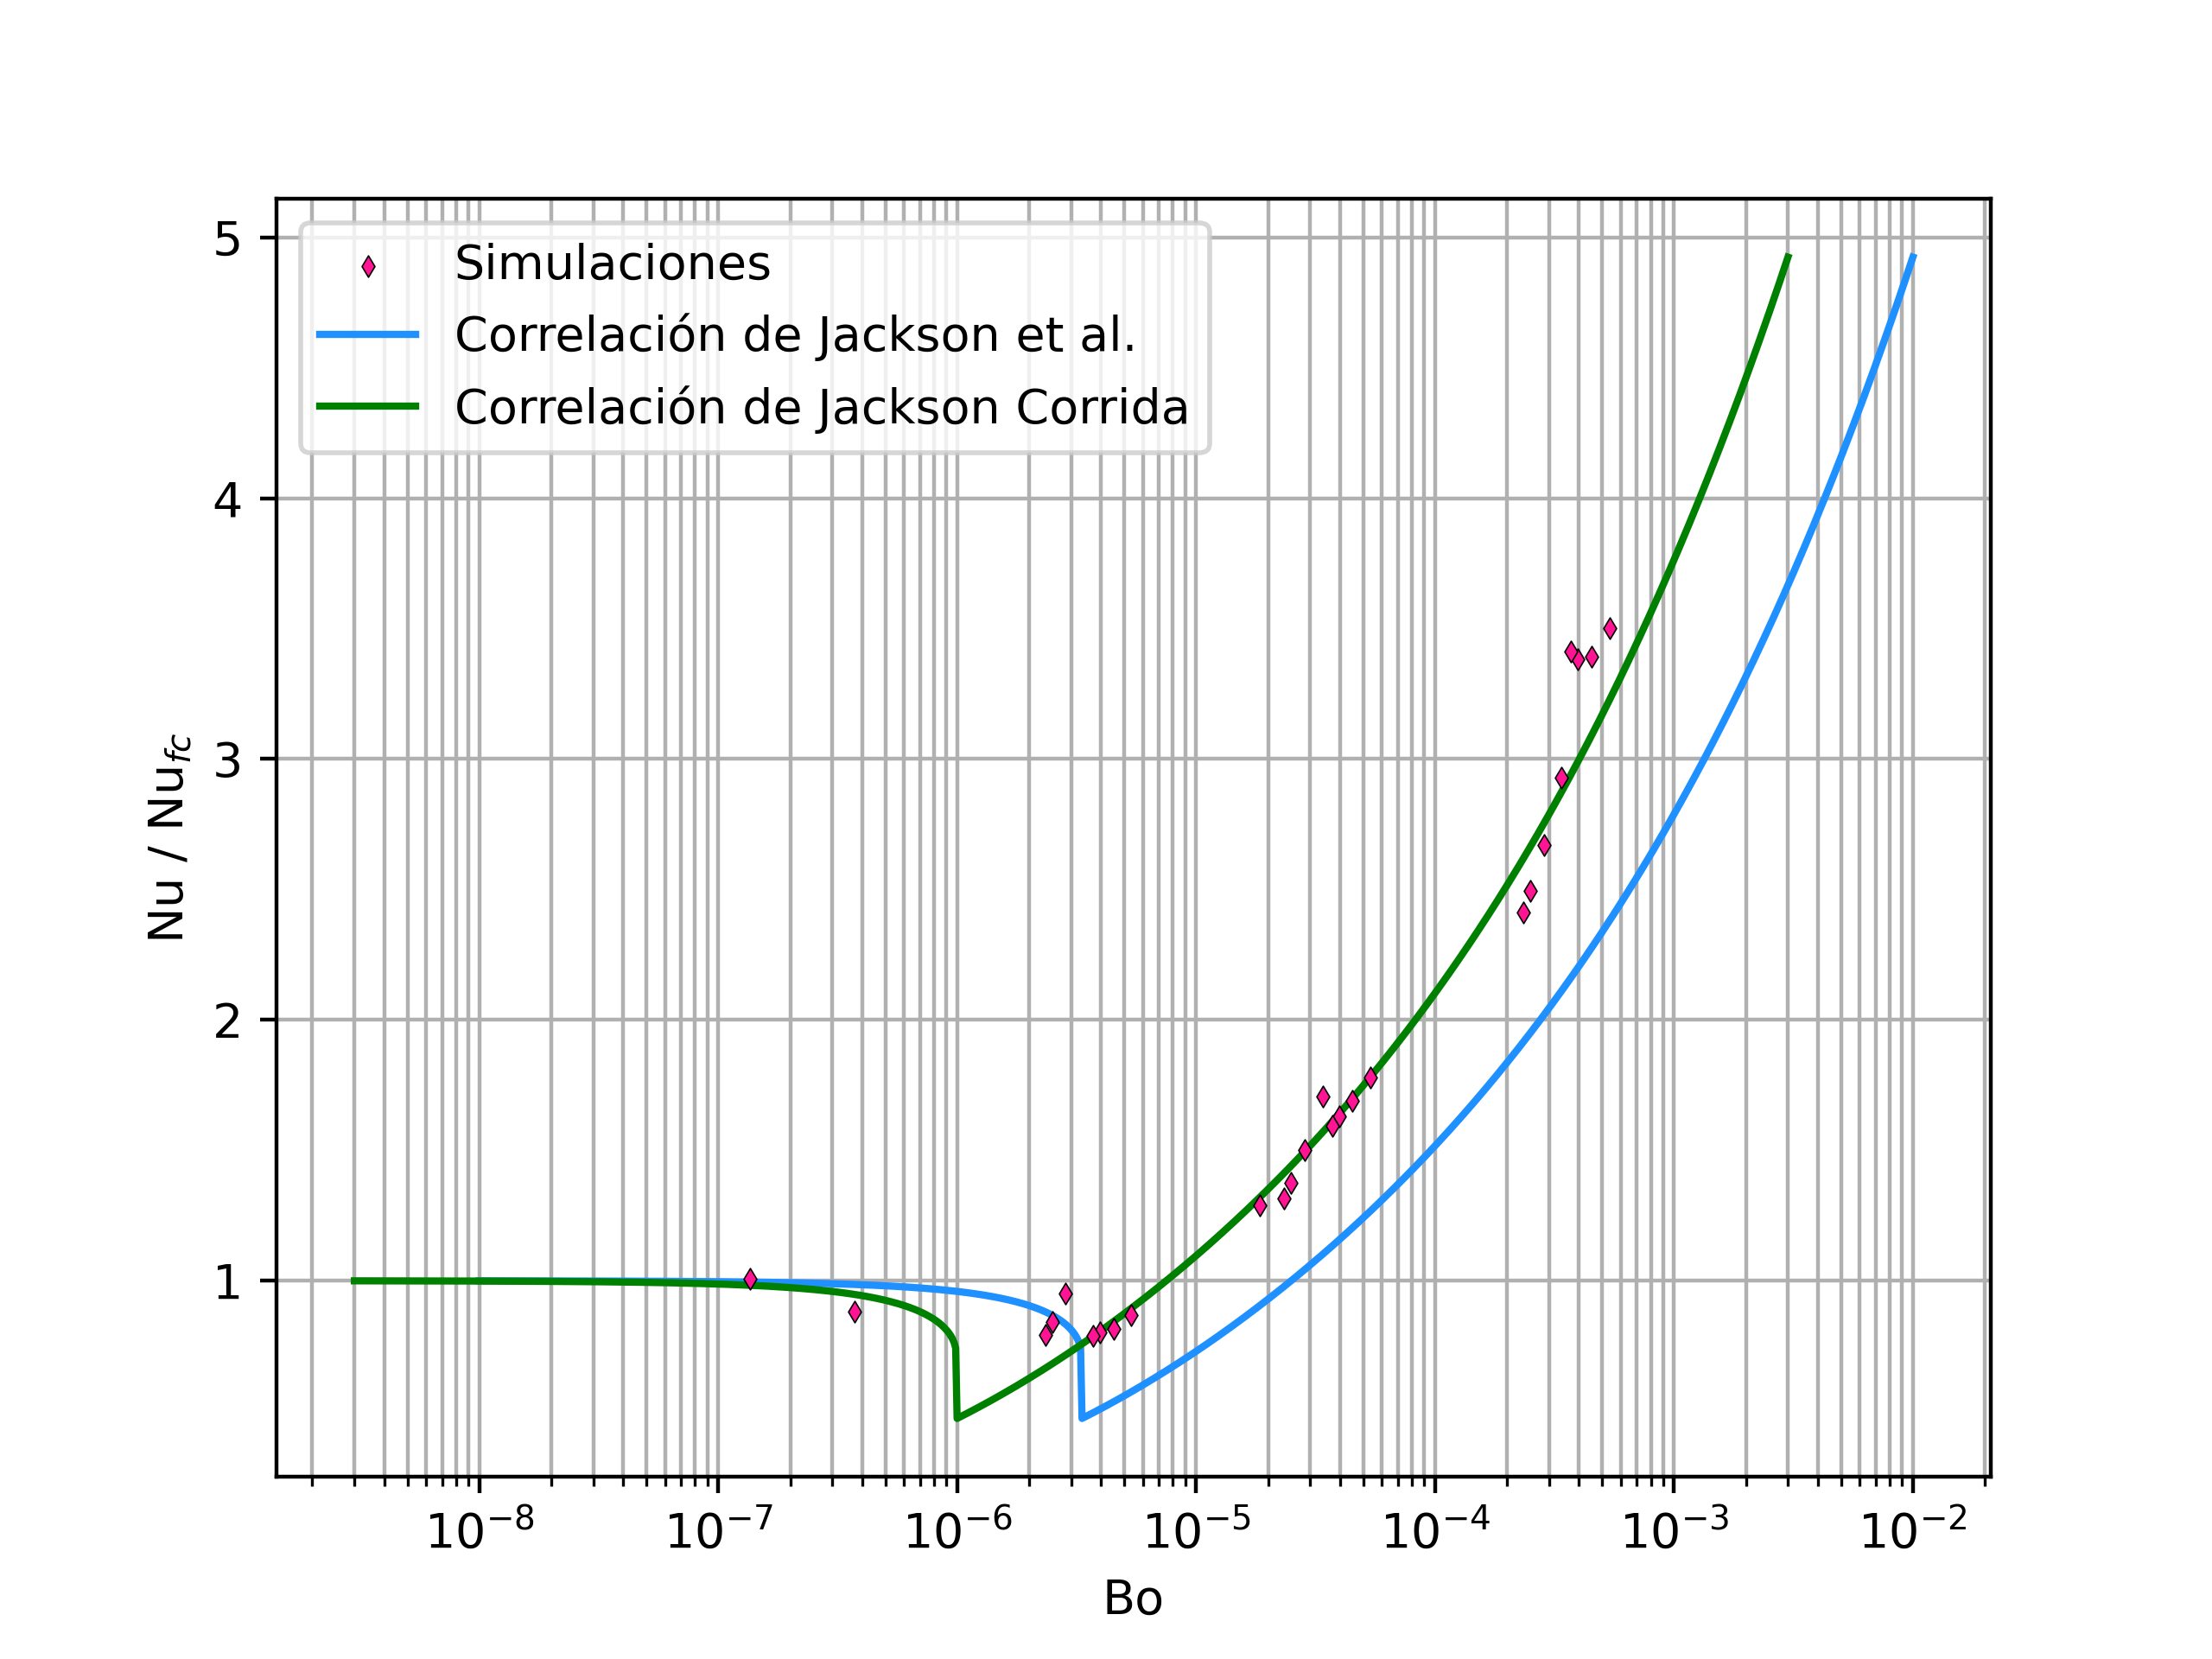
\includegraphics[width=0.49\textwidth]{figures/cap5/nusselt_corr/Nu_vs_Bo_Jackson.png}
%    	\label{fig:nu_vs_bo}}
%  \subfloat[]{
%    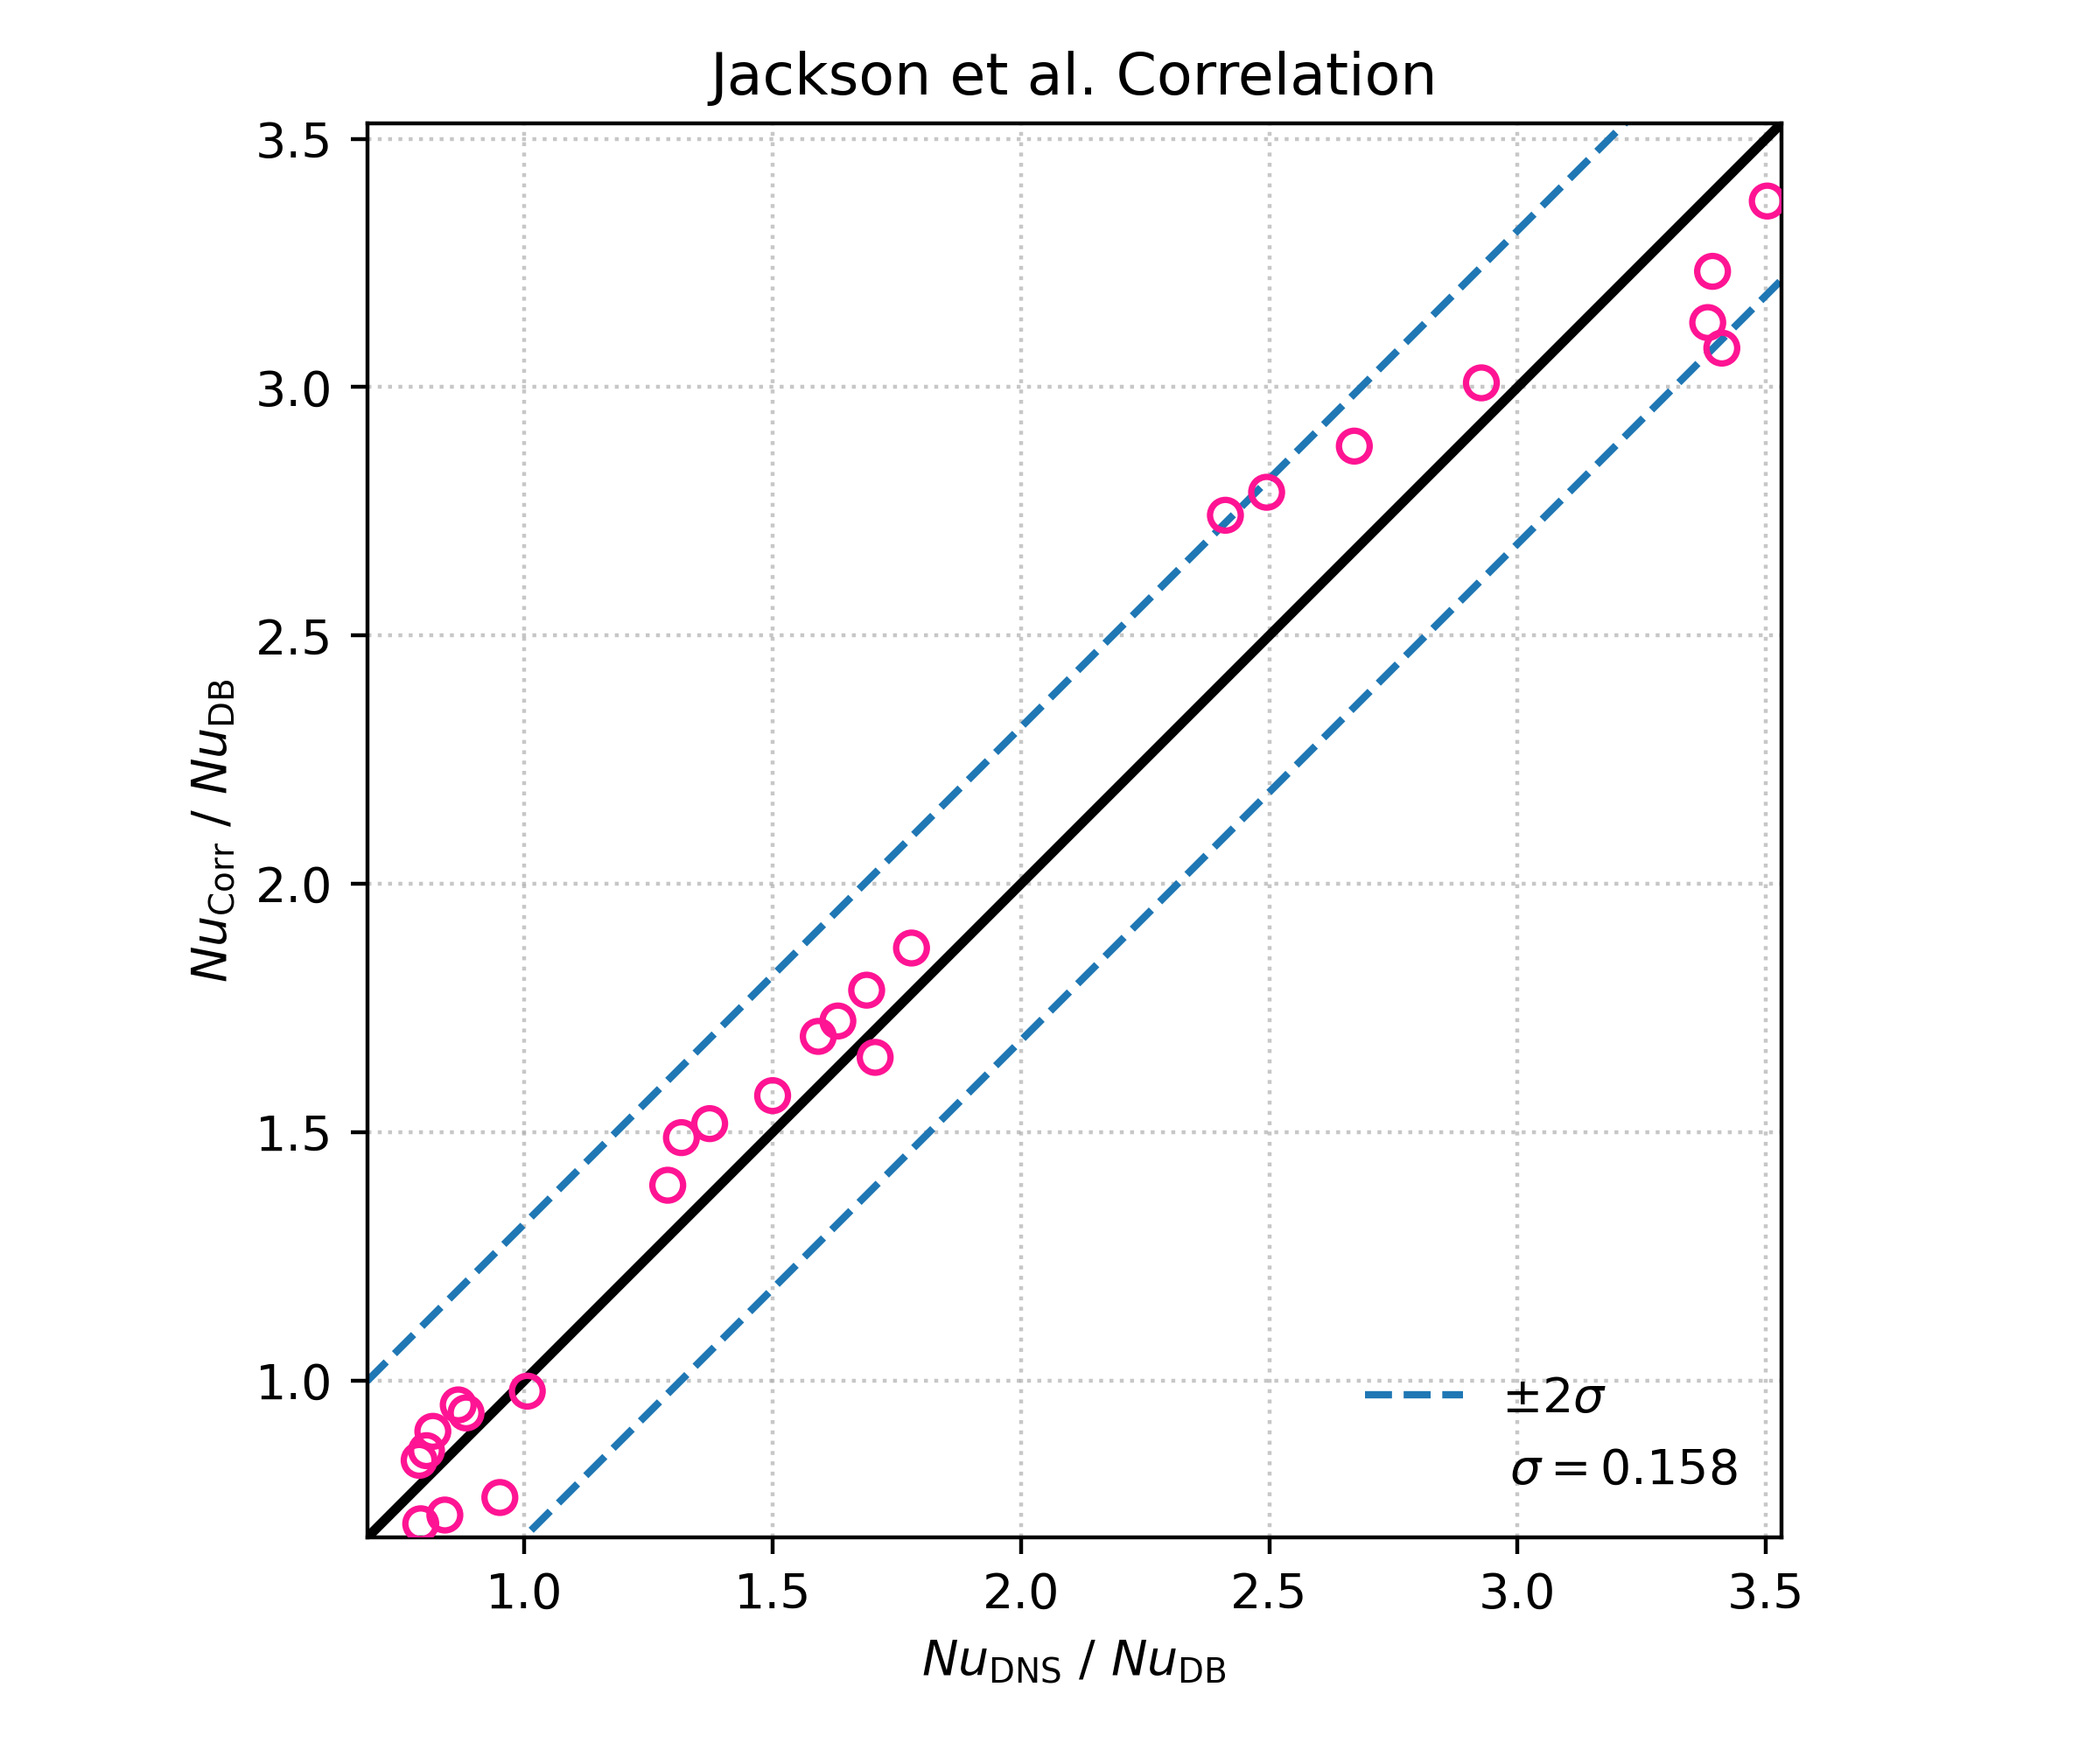
\includegraphics[width=0.49\textwidth]{figures/cap5/nusselt_corr/jackson_parity.png}
%    	\label{fig:parity}}
%    
%  \caption{Aquí $Bo = Gr / (Re^{3,425} Pr^{0,8})$}
%  \label{fig:nusselt}
%\end{figure}
%
%La caída del número de Nu con el aumento de la fuerza boyante puede interpretarse en términos del perfil de velocidad en la dirección de la corriente. En la sección \ref{sec:velo_temp} se comentó que cuando la convección natural y la convección forzada actúan en la misma dirección el fluido es acelerado en las zonas cercanas a las paredes y, en virtud de la conservación de masa, el flujo se desacelera en la región central. En virtud de esta premisa es posible acercarse a un entendimiento cualitativo. De acuerdo al modelo de Prandtl \cite{Prandtl1942}, la transferencia de calor ocurre mediante 2 mecanísmo principales: transferencia por conducción en la subcapa viscosa y por el flujo de calor turbulento en la dirección normal a la pared, esto es, $q''_y \aprox \rho \hspace{0.5mm} c_P \hspace{0.5mm} \langle u^{*'}_y \theta^{*'} \rangle$. De acuerdo a Aicher y Martin \cite{aicher1997}, en la zona cercana al borde de la capa viscosa, el flujo $q''_y$ es proporcional a la producción de turbulencia el cuál es la suma de la \textit{Shear-Production} y \textit{Buoyancy-Production}, cantidades (o \textit{budgets}) provenientes del balance de la cinética turbulenta $k$ (Apéndice \ref{apen:budgets}). En este sentido, la producción de turbulencia dependerá de la diferencia de velocidades entre el centro del canal y la zona próxima a la pared.
%
%Así, dado que la boyancia produce un aumento de la velocidad cerca de las paredes, es posible apreciar una rango de Ri$b$ ($10^{-6}$ $\lesssim$ Bo $\lesssim$ $3 \times 10^{-5}$ de la Figura \ref{fig:nu_vs_bo}) para los cuales ésta diferencia es, o bien cero, o bien muy pequeña. A medida que la fuerza boyante sigue incrementando, dicha diferencia de velocidades (o gradiente) crece, y en consecuencia, aumenta la producción de turbulencia, el flujo de calor turbulento normal y transferencia de calor que se refeja en un aumento del Nu.  
%
%
%
%


%\begin{figure}[H]
%  \centering
%   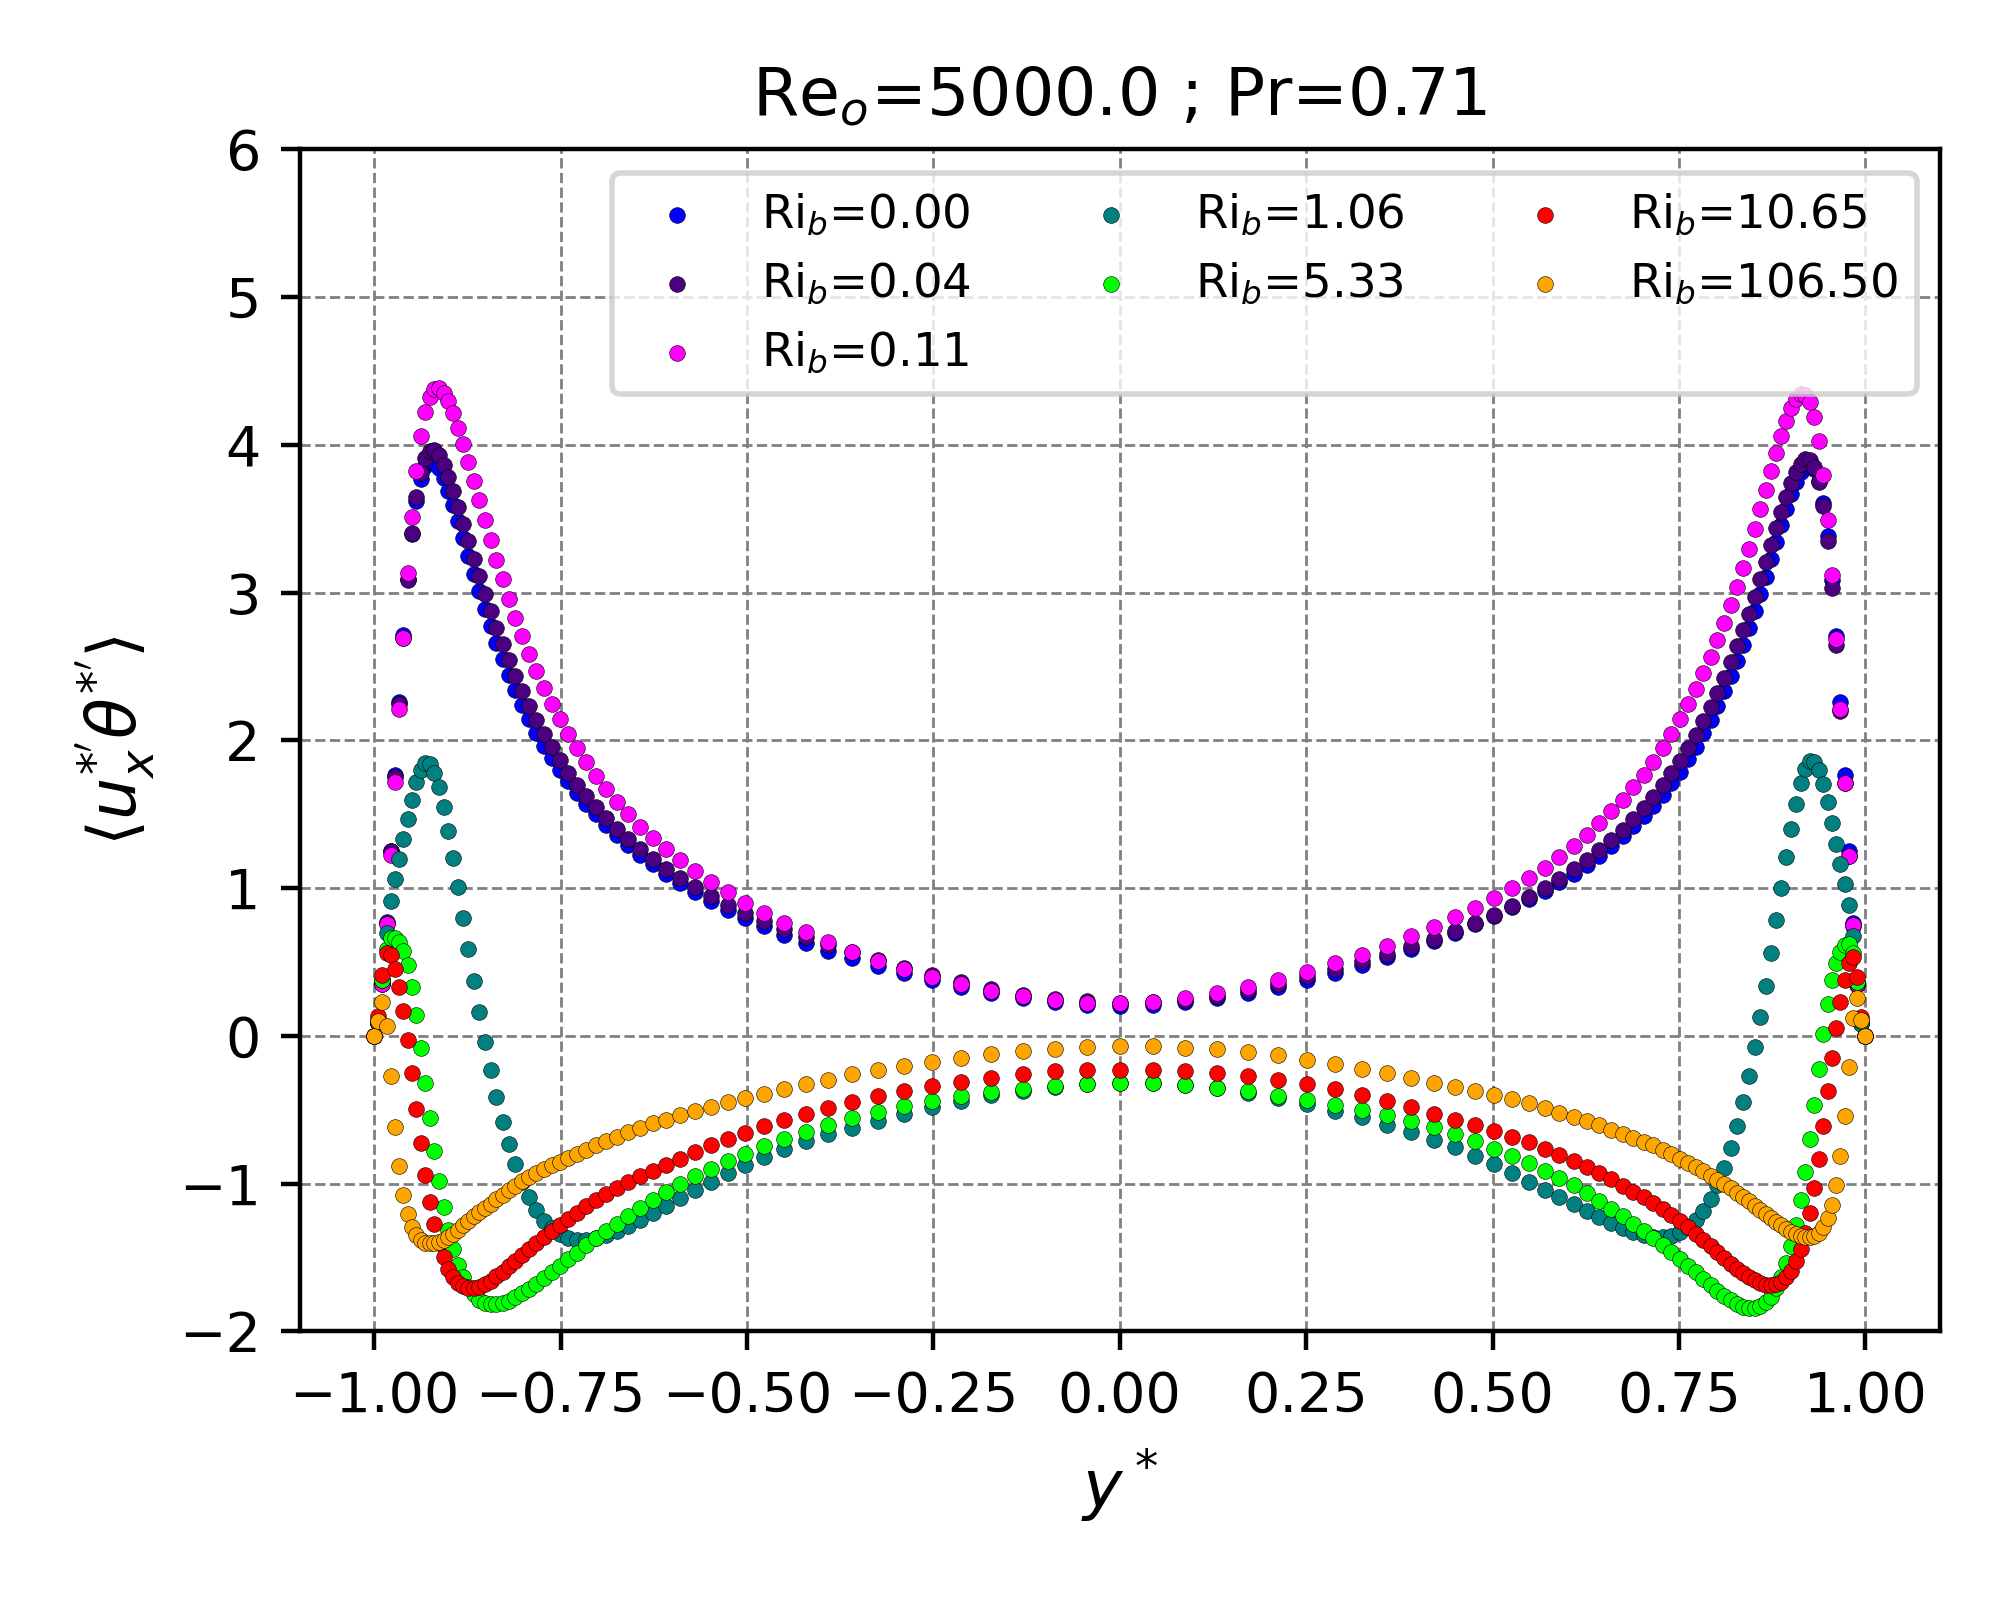
\includegraphics[width=0.6\textwidth]{figures/cap5/Re5000-Pr071/uphif_profile.png}
%   	\label{fig:uphif-Re5000-Pr071}
%  \caption{\textcolor{red}{Acá va el flujo de calor turbulento normal a la pared ... solo que todavía no pude hacerlo porque el cluster está inactivo ...}}
%\end{figure}



\newpage
\section{Número de Nusselt} \label{sec:nu}

Desde una perspectiva ingenieril, el número de Nusselt (Nu) es un indicador clave de la eficiencia de la transferencia de calor. Su definición se presenta en la ecuación \ref{eq:nu}, donde $\langle \theta_b \rangle$ es la temperatura \textit{bulk} (ecuación \ref{eq:tita_bulk}).

\begin{equation}
\text{Nu} = \frac{h L}{k} = \frac{2d}{k} \frac{q''_w}{\langle \theta_b \rangle} = \frac{4}{3} \frac{Re_o Pr}{\langle \theta^*_b \rangle}	
\label{eq:nu}
\end{equation}

\begin{equation}
\langle \theta_b \rangle = \frac{\int_{-d}^{+d} \langle u_x \theta \rangle \, dy}{\int_{-d}^{+d} \langle u_x \rangle \, dy} = \frac{\int_{-d}^{+d} \langle u_x \theta \rangle }{2d \, U_b}
\label{eq:tita_bulk}
\end{equation}

La Figura \ref{fig:nu_vs_bo} muestra los valores de Nu obtenidos en función del número de boyancia Bo (ecuación \ref{eq:jackson_bo}), que cuantifica la relación entre las fuerzas boyantes y la fuerza impulsora de la convección forzada. Estos resultados se comparan con la correlación de Jackson et al. \cite{jackson1989studies} (ecuación \ref{eq:jackson_corr}). Los valores de Nu se normalizan con el valor correspondiente a convección forzada pura, Nu$_{fc}$, evaluado mediante la correlación de Dittus-Boelter \cite{incropera}. También se añaden datos provenientes de simulaciones DNS \cite{you2003direct} que se alinean con la misma tendencia.

En la Figura \ref{fig:parity} se presenta un gráfico de paridad entre $Nu_{\text{DNS}}/Nu_{DB}$ (eje $x$) y $Nu_{\text{corr}}/Nu_{DB}$ (eje $y$). La línea negra indica el acuerdo perfecto ($y=x$) y las líneas azules punteadas delimitan la banda de $\pm2\sigma$ (con $\sigma$=0.158). La concentración de puntos dentro de esta banda confirma que la correlación de Jackson reproduce con buena precisión los valores simulados.

A partir de la Figura \ref{fig:nu_vs_bo} se distinguen tres regiones:

\begin{itemize}
  \item[$\bullet$] Bo $\lesssim 10^{-6}$: Nu se mantiene prácticamente igual a Nu$_{fc}$; domina la convección forzada.
  \item[$\bullet$] $10^{-6} \lesssim$ Bo $\lesssim 3 \times 10^{-5}$: Nu desciende y luego se recupera, indicando una zona donde la transferencia de calor empeora temporalmente respecto al caso puramente forzado.
  \item[$\bullet$] Bo $\gtrsim 3 \times 10^{-5}$: Nu crece de forma marcada, impulsado por la mayor relevancia de la convección natural.
\end{itemize}

\begin{equation}
\text{Bo}= \frac{Gr*}{\text{Re}_D^{3.425} \hspace*{1mm} \text{Pr}^{0.8}}
\label{eq:jackson_bo}
\end{equation}

\begin{equation}
\frac{\text{Nu}}{\text{Nu}_{fc}} =
\left\vert 1 - 8 \times 10^4 \hspace*{0.5mm} \text{Bo}
\left( \frac{\text{Nu}}{\text{Nu}_{fc}} \right)^{-2} \right\vert^{0.46}
\label{eq:jackson_corr}
\end{equation}

\begin{figure}[H]
  \centering
  \subfloat[]{
    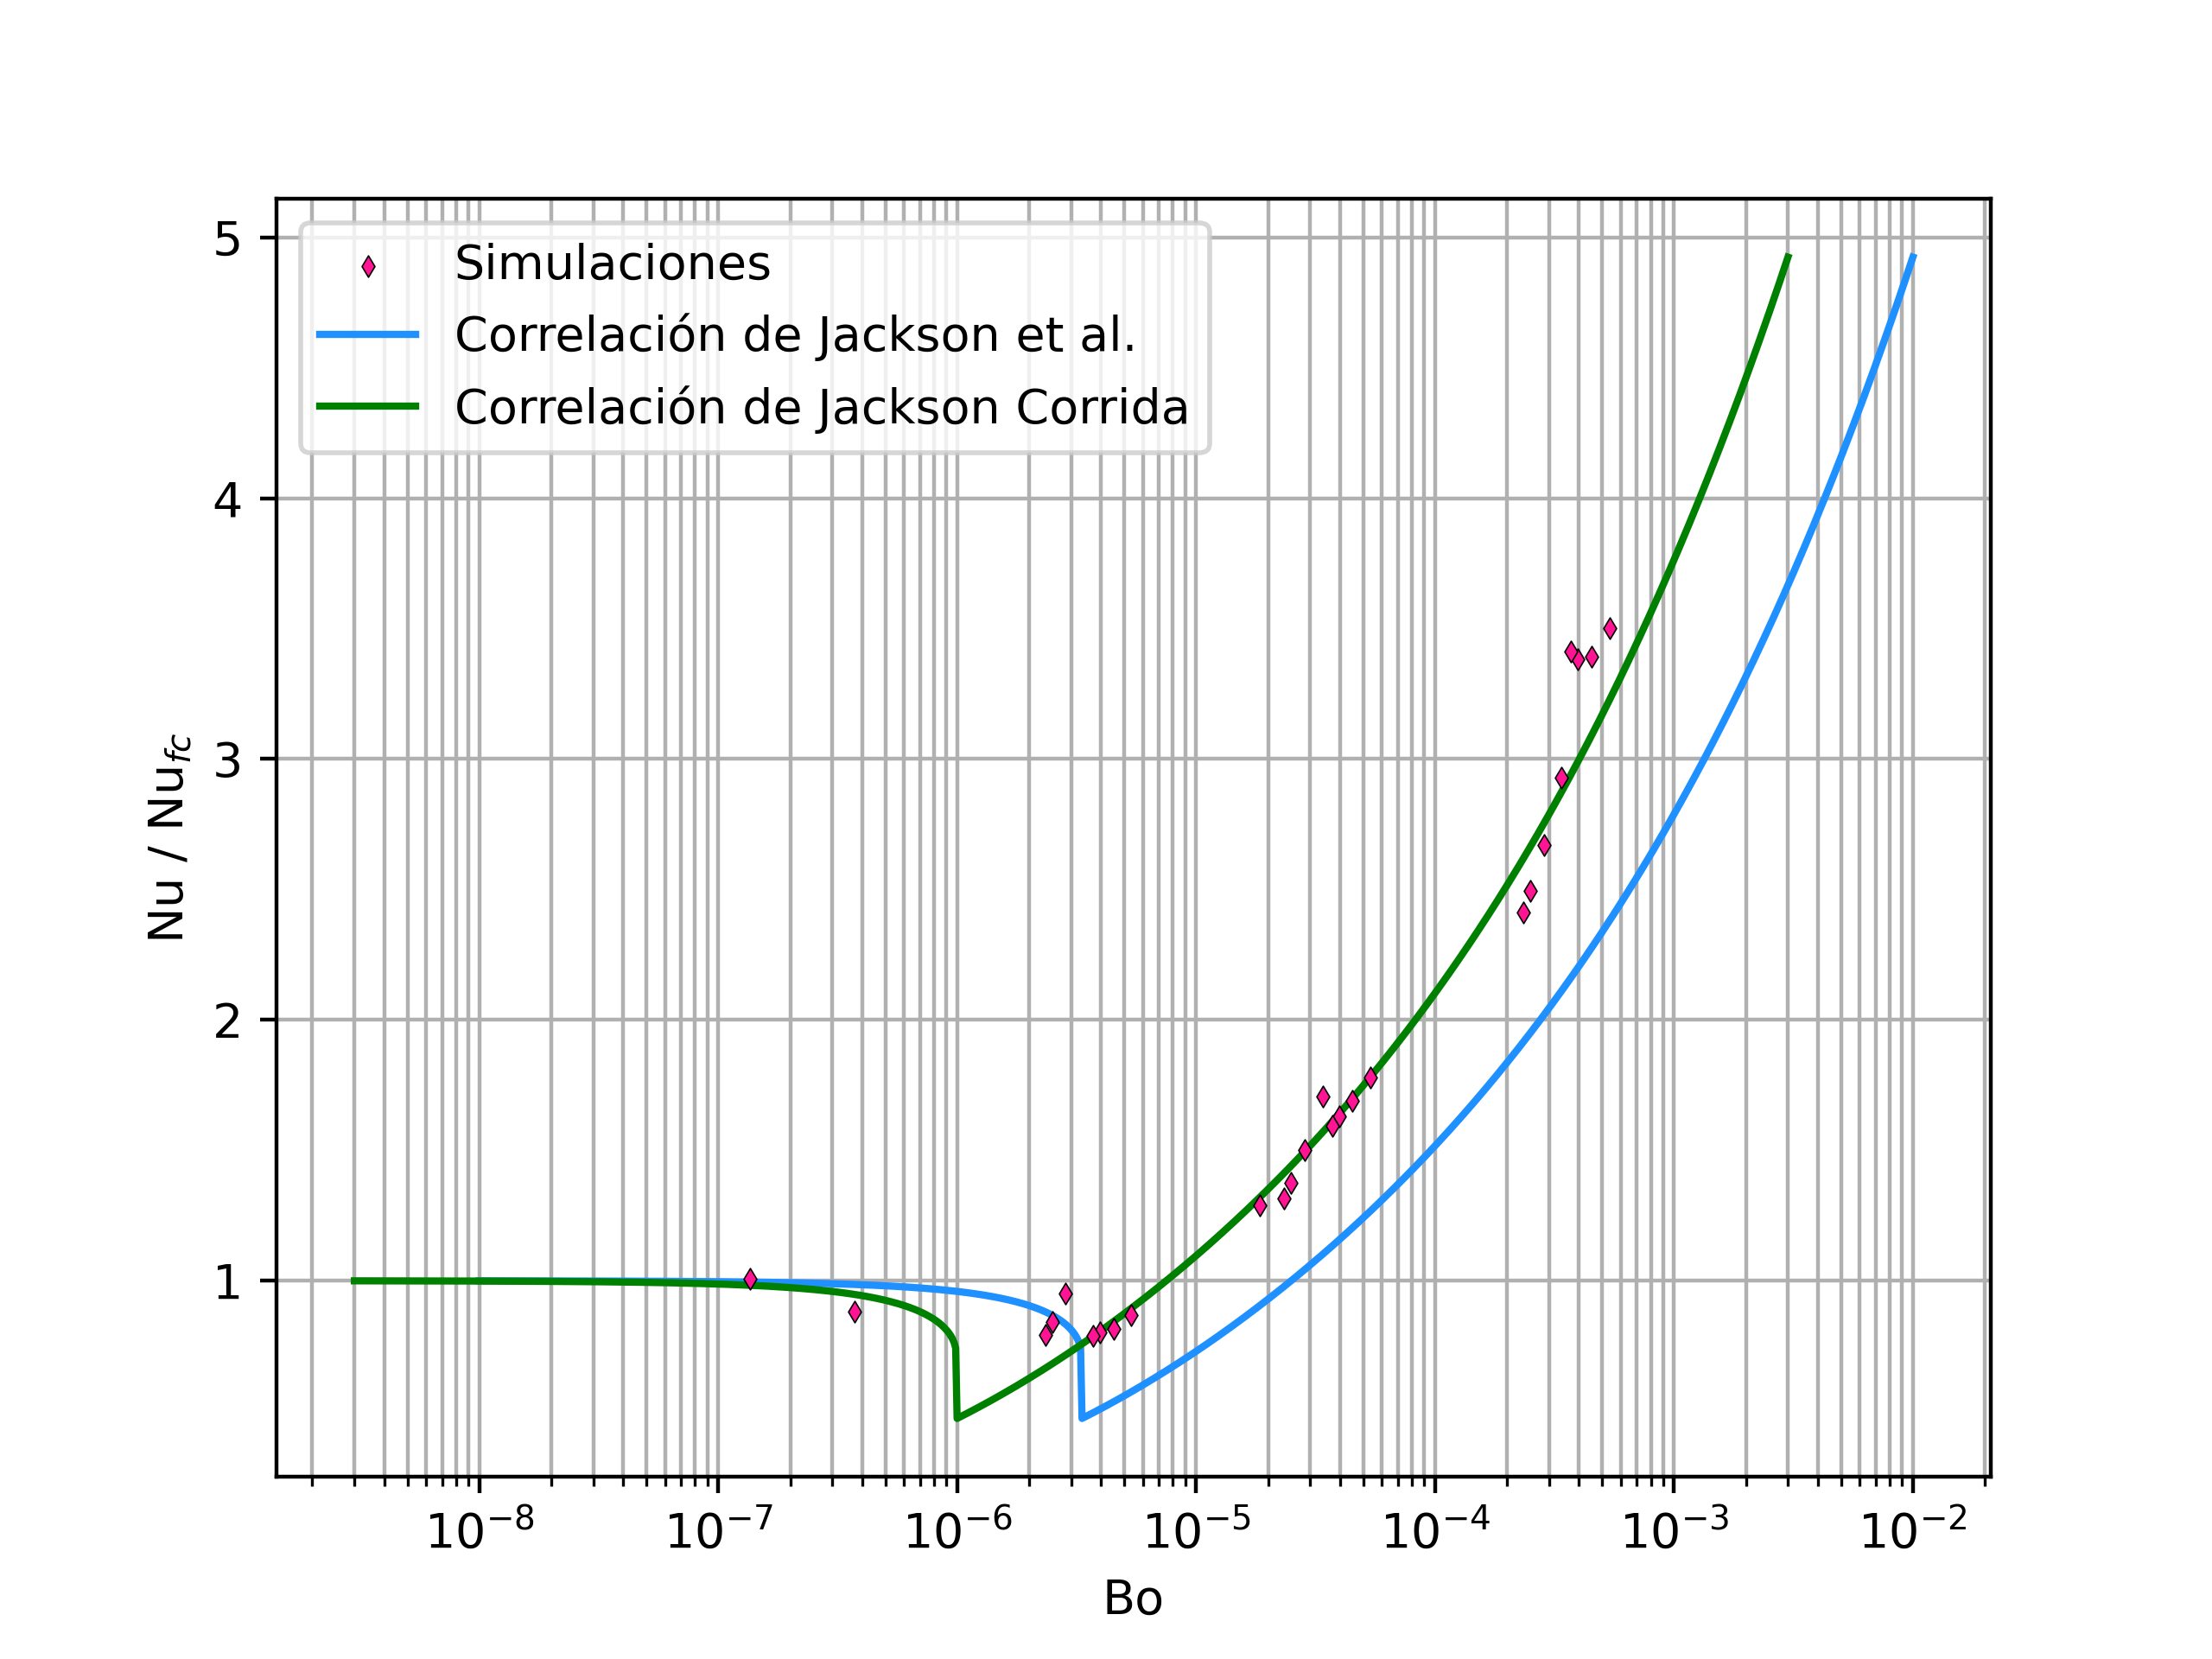
\includegraphics[width=0.49\textwidth]{figures/cap5/nusselt_corr/Nu_vs_Bo_Jackson.png}
    \label{fig:nu_vs_bo}}
  \subfloat[]{
    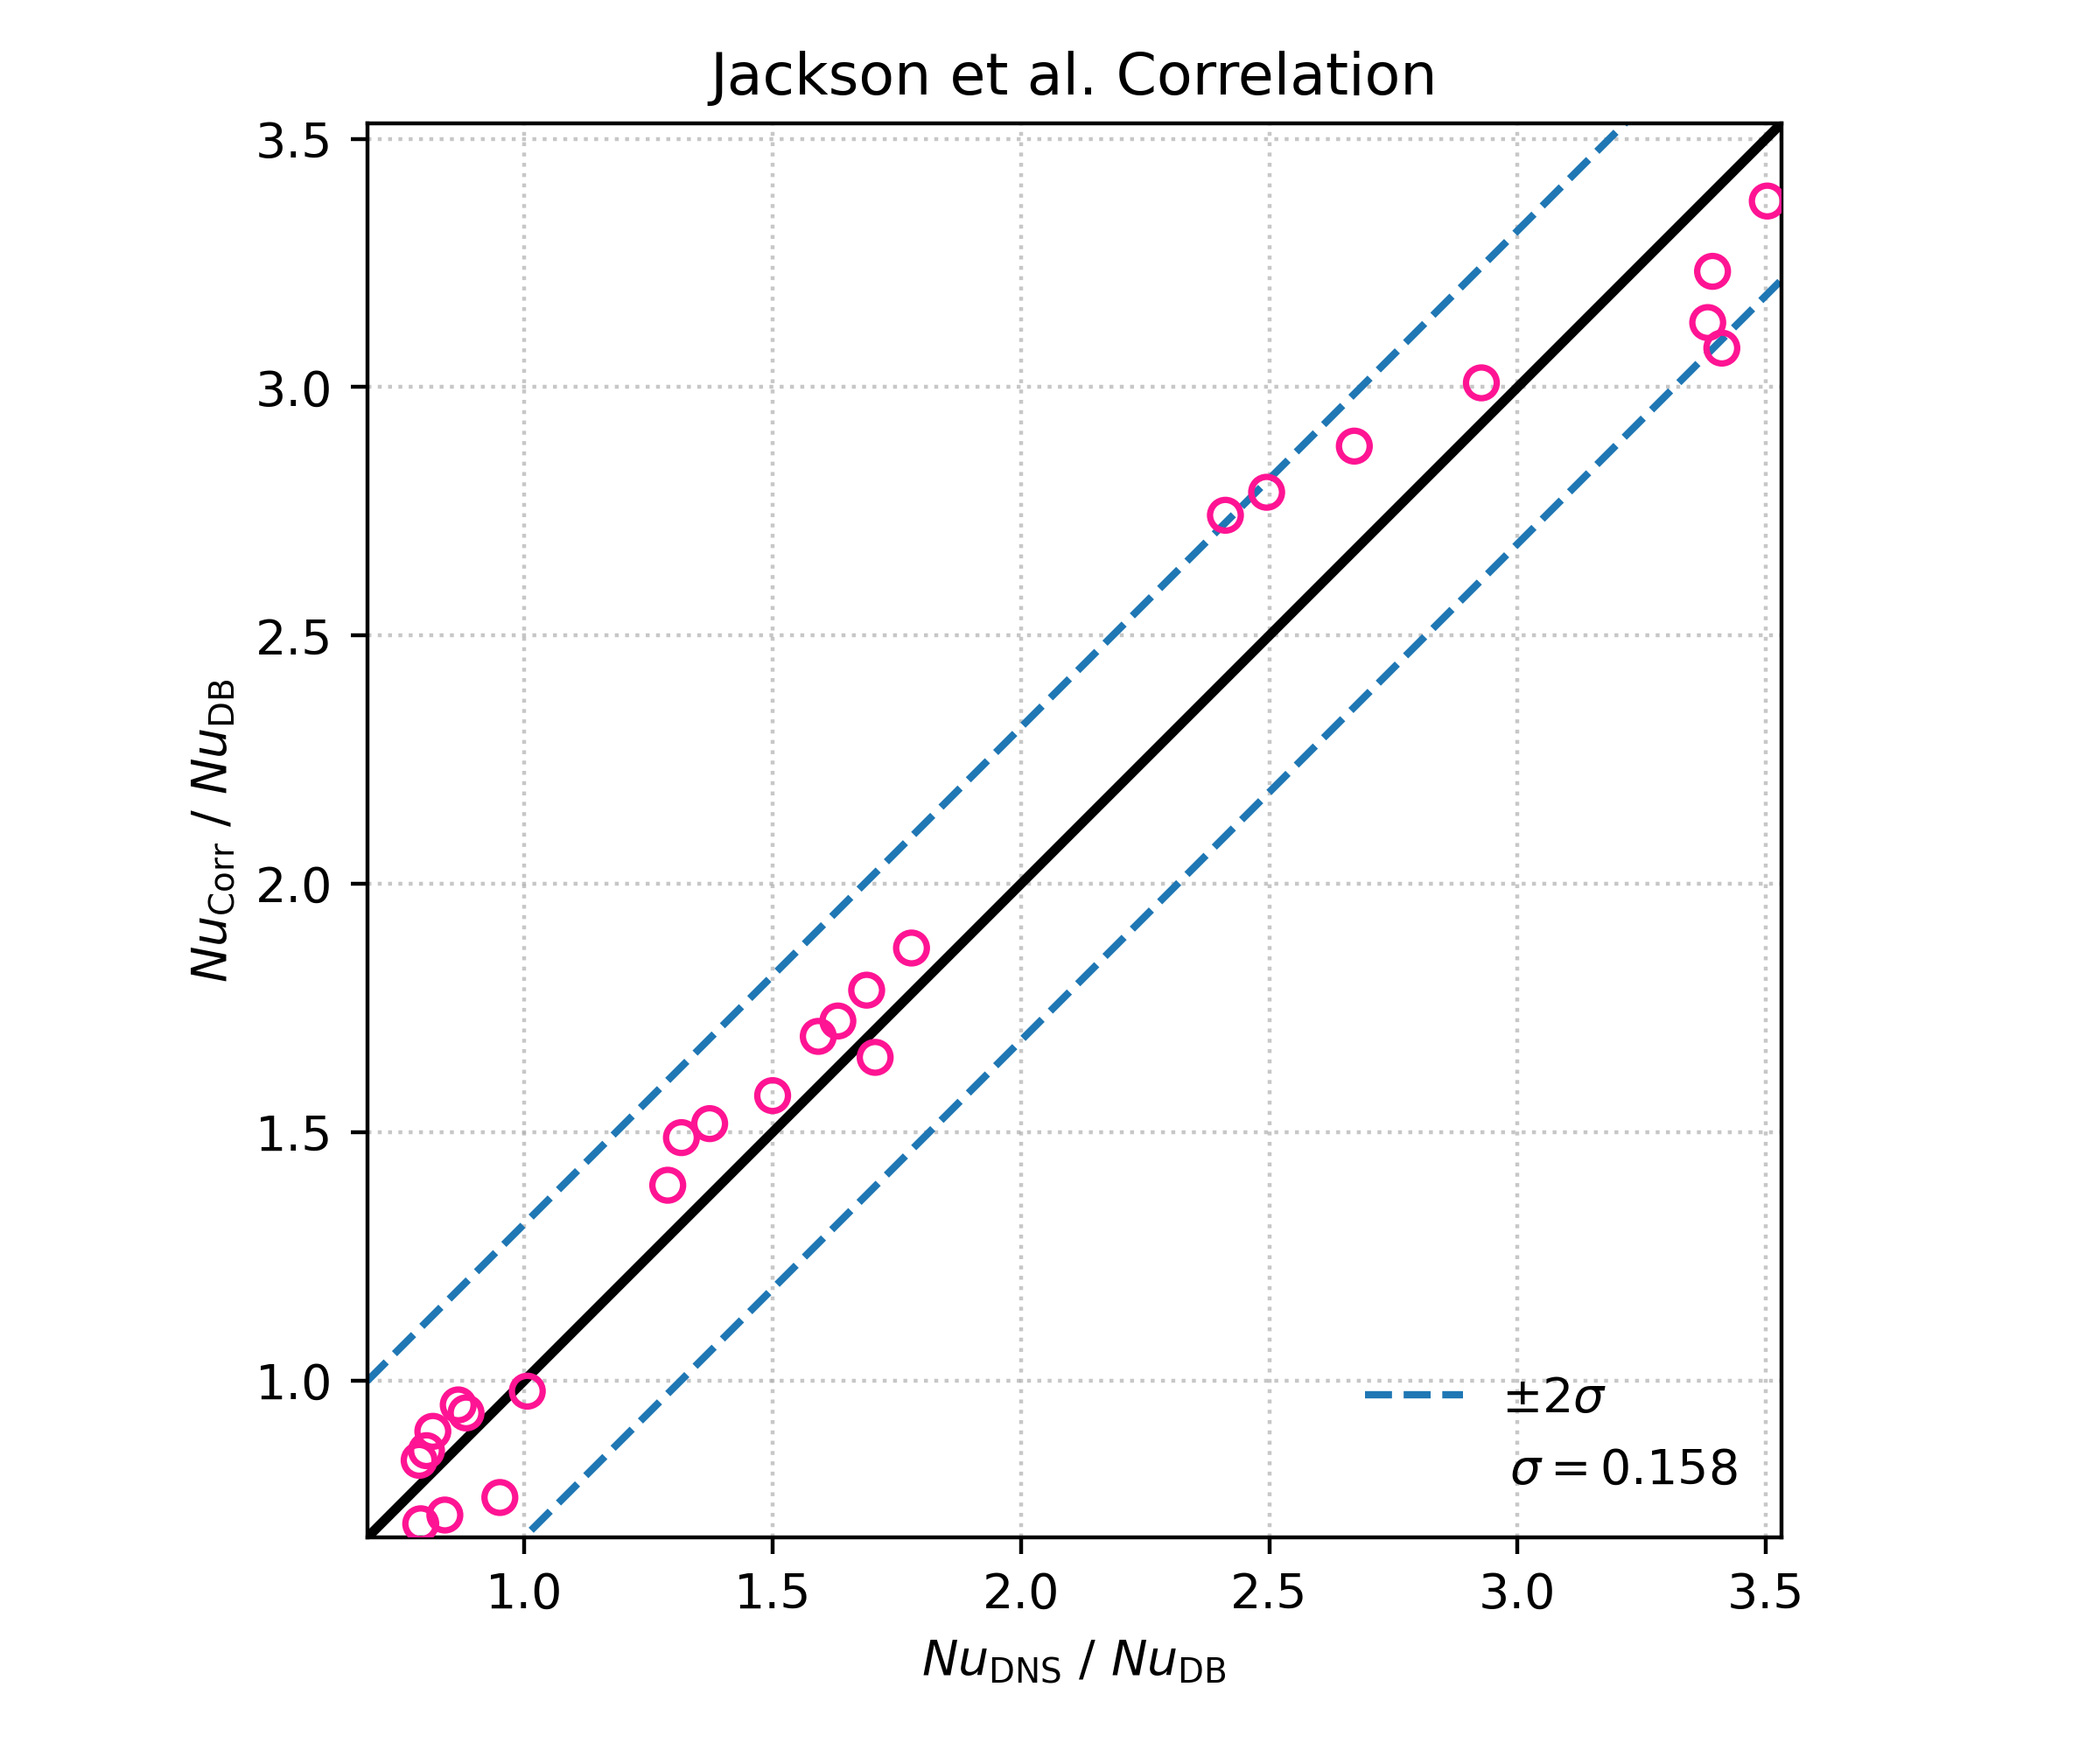
\includegraphics[width=0.49\textwidth]{figures/cap5/nusselt_corr/jackson_parity.png}
    \label{fig:parity}}
  \caption{\textbf{(a)} Número de Nusselt normalizado vs Bo; \textbf{(b)} paridad con la correlación de Jackson \textit{et al.}}
  \label{fig:nusselt}
\end{figure}



La disminución de Nu al aumentar la fuerza boyante puede entenderse a partir del perfil de velocidad en la dirección del flujo. Como se menciona en la sección \ref{sec:velo_temp}, cuando la convección natural y forzada actúan en la misma dirección, el fluido se acelera junto a las paredes y, por conservación de masa, se desacelera en la región central. En virtud de esta premisa, es posible acercarse a un entendimiento cualitativo. De acuerdo al modelo de Prandtl \cite{Prandtl1942}, la transferencia de calor se divide en dos mecanismos principales: (i) conducción en la subcapa viscosa y (ii) flujo de calor turbulento normal a la pared, $q''_y \approx \rho \, c_P \, \langle u^{*'}_y \theta^{*'} \rangle$. Algunos autores \cite{aicher1997, hall1969laminarization} sugieren que en el borde de la subcapa viscosa,  $q''_y$ es proporcional a la producción de turbulencia, cuya principal contribución recae en la producción por cizalla $\mathcal{P}$ (\textit{Shear-Production}). Sin embargo, también debe considerarse (aunque en menor medida) la contribución de la producción por boyancia $\mathcal{B}$ (\textit{Buoyancy-Production}). Los términos $\mathcal{P}$ y $\mathcal{B}$ provienen del balance de energía cinética turbulenta $k$  (véase el Apéndice \ref{apen:budgets}). El primero está ligado a diferencia de velocidades entre el centro del canal y la zona próxima a la pared, es decir, a un gradiente de velocidades.

Así, es posible apreciar un rango de Ri$_b$, correspondiente al intervalo $10^{-6}$ $\lesssim$ Bo $\lesssim$ $3 \times 10^{-5}$ en la Figura \ref{fig:nu_vs_bo}, para los cuales la aceleración inducida por la boyancia produce que esta diferencia de velocidades, o bien sea cero, o bien sea muy pequeña. Como consecuencia, disminuyen la producción turbulenta, el flujo de calor turbulento y, por lo tanto, Nu. Cuando la fuerza boyante continúa creciendo más allá de este intervalo, el gradiente de velocidad vuelve a incrementarse, la producción de turbulencia se intensifica y tanto $q''_y$ como Nu aumentan nuevamente. 

Esta última cuestión puede confirmarse al observar las Figuras \ref{fig:shear_prod} y \ref{fig:buoya_prod} donde se exponen los perfiles medios de $\mathcal{P}$ y $\mathcal{B}$, respectivamente, de los casos con Re$_o$=5000 y Pr=0.71. Se aprecia que valores moderados bajos de Ri$_b$ los perfiles tienen a decaer cerca de la pared, reduciendo la producción de turbulencia. Además, en general, se observa que la magnitud $\mathcal{B}$ es al menos un orden de magnitud menor y porque no tiene un rol tan relevante en la producción de turbulencia.

\begin{figure}[H]
  \centering
  \subfloat[]{
    \includegraphics[width=0.49\textwidth]{figures/cap5/Re5000-Pr071-Ri1Em3_shear_prod.png}
    \label{fig:shear_prod}}
  \subfloat[]{
    \includegraphics[width=0.49\textwidth]{figures/cap5/Re5000-Pr071-Ri1Em3_buoya_prod.png}
    \label{fig:buoya_prod}}
  \caption{Producción de energía cinética turbulenta: \textbf{(a)} componente por cizalla $\mathcal{P}$ y \textbf{(b)} contribución de la fuerza boyante $\mathcal{B}$.}
  \label{fig:budgets_prod}
\end{figure}


\newpage
\section{Factor de Fricción de Darcy}

En esta sección se analizan los resultados del coeficiente de fricción de Darcy. El mismo se define por la relación
\begin{equation}
f = 8 \frac{ \overline{\tau_w}}{\hspace{0.5mm} \rho \hspace{0.5mm} {U_b}^2 }  = \frac{18}{\text{Re}_o} \left.\frac{d \langle u^*_x \rangle}{dy}\right\vert_{wall} \text{.}
\label{eq:darcy}
\end{equation}
La Figura \ref{fig:darcy_vs_bo} recoge los valores de $f$ obtenidos en nuestras simulaciones DNS para una amplia gama de números de Boyancia (ecuación \ref{eq:jackson_bo}). Se incluyen, además, datos experimentales de Parlatan et al. \cite{parlatan1996buoyancy} y de DNS de You et al. \cite{you2003direct}. La coincidencia de tendencias entre los tres conjuntos de datos es excelente. Por otro lado, la literatura ofrece pocas correlaciones para $f$ (o para el factor de Fanning) en flujo turbulento completamente desarrollado bajo régimen de convección mixta. Partiendo del planteo de Easby \textit{et al.} \cite{easby1978effect}, se propone una nueva forma funcional, dada por la ecuación \ref{eq:fcorr}, cuyos parámetros se ajustan con nuestros resultados.
\begin{equation}
f_{corr} = C_1 + C_2 \hspace*{0.5mm} \text{Bo}^n
\label{eq:fcorr}
\end{equation}

\begin{small}
$$
C_1 = 0.03071701 \quad ; \quad C_2 = 10.03126205 \quad ; \quad n = 0.56152207
$$
\end{small}

La Figura \ref{fig:darcy_parity} muestra el gráfico de paridad $f_{\text{DNS}}$ frente a $f_{\text{corr}}$. La desviación estándar es $\sigma$=0.018 y el total de nuestros puntos se sitúa dentro de la banda de error, lo que confirma la fiabilidad de la correlación incluso al compararla con los datos de referencia externos.

\begin{figure}[H]
  \centering
  \subfloat[]{
    \includegraphics[width=0.49\textwidth]{figures/cap5/darcy/darcy_vs_Bo.png}
    \label{fig:darcy_vs_bo}}
  \subfloat[]{
    \includegraphics[width=0.49\textwidth]{figures/cap5/darcy/darcy_parity.png}
    \label{fig:darcy_parity}}
  \caption{Coeficiente de fricción de Darcy vs Bo y correlación propuesta; el ajuste reproduce los datos DNS/experimentales con $\sigma$ = 0.018.}
  \label{fig:nusselt}
\end{figure}

El incremento de $f$ con la boyancia parece, a priori, contraintuitivo: al actuar la fuerza boyante en la misma dirección del flujo cabría esperar menores pérdidas de carga. Sin embargo, los perfiles de velocidad mostrados en la sección \ref{sec:velo_temp} evidencian que la boyancia acelera el fluido en las zonas próximas a la pared, lo que incrementa la pendiente $d \langle u^*_x \rangle / dx^*$ y, por ende, la tensión cortante media $\overline{\tau_w}$. Este aumento local de cizalla compensa, e incluso supera, la ayuda proporcionada por la fuerza boyante, resultando en un valor mayor de $f$.


\section{Sumario de los principales hallazgos}

\begin{itemize}

\item \textbf{Perfiles de velocidad:} la fuerza boyante genera perfiles tipo ``M'' y desplaza el máximo de $\langle u_x\rangle$ hacia la pared.

\item \textbf{Perfiles de temperatura:} la mezcla inducida por la flotación ``aplana'' la temperatura media y reduce su fluctuaciones en el núcleo del canal.

\item \textbf{Degradación y mejora de Nu:} existe un intervalo $10^{-6}!\lesssim!Bo!\lesssim!3!\times!10^{-5}$ donde $Nu$ cae; fuera de él la transferencia se recupera y supera el caso puramente forzado.

\item \textbf{Mecanismo energético:} la caída de Nu coincide con una disminución en la producción de turbulencia cerca de la pared.

\item \textbf{Factor de Darcy creciente:} pese a la asistencia de la boyancia, el gradiente de velocidad en la pared aumenta y eleva el factor de Darcy; la correlación $f_{\text{corr}}=C_1+C_2 Bo^n$ reproduce los datos simulados propios, y los datos de referencia, con buena fidelidad.

\item \textbf{Efecto del Prandtl:} para Pr=0.071 la ley lineal de temperatura $\langle\theta^*\rangle \simeq \text{Pr} y^+$ se mantiene hasta $y^+ \approx 30$, mientras que para Pr=0.71 termina a $y^+ \approx 7$.
\end{itemize}
\chapter{Convección Mixta En Transición Laminar-Turbulenta} \label{cap:transicion}

En el presente capítulo se examina la transición laminar-turbulenta en convección mixta en un canal de placas paralelas mediante simulaciones DNS. El mismo se organiza en tres partes: (i) la exploración de distintas condiciones iniciales mediante la evolución temporal de magnitudes de interés (TKE y Re$_{\tau}$) contemplando dos valores del número de Richardson Ri$_b$ (casos A y B); (ii) un análisis detallado del caso correspondiente al Ri$_b$ más bajo simulado (ensayo A-C10); (iii) un análisis detallado del caso correspondiente al Ri$_b$ más alto simulado (ensayo B-C2).

En los ensayos A-C10 y B-C2 se consideran las siguientes magnitudes de interés: la energía cinética turbulenta (TKE) y la varianza de la temperatura adimensional; perfiles de velocidad y de temperatura adimensional en instantes representativos; el factor de fricción de Darcy y número de Nusselt. Este conjunto de métricas permite vincular la dinámica de la transición con su impacto termo-hidrodinámico y con el acercamiento a los estados de referencia completamente desarrollados.

En los ensayos con Ri$_b$ más bajo ($\text{Ri}_b=0\text{.}04$) se requirió emplear una combinación de perturbaciones bidimensionales y tridimensionales para desencadenar la transición. Por su parte, aquellos ensayos con Ri$_b$ más alto ($\text{Ri}_b=1\text{.}06$), si bien también se consideraron condiciones iniciales construidas con combinaciones de ondas 2D/3D, fue posible inestabilizar el flujo empleando únicamente ondas 2D. 

En el ensayo A-C10, en una etapa inicial ($t^*\lesssim 400$), la evolución temporal de las \linebreak cantidades se caracteriza por experimentar mínimos y/o máximos locales y absolutos, \linebreak salvo en el número de Nusselt que en esta etapa se mantiene prácticamente constante. Luego, estas magnitudes tienden hacia el estado turbulento desarrollado. En particular, las cantidades asociadas al campo hidrodinámico del sistema evolucionan a mayor ritmo respecto de aquellas cantidades asociadas al campo térmico. Al inspeccionar los perfiles de velocidad y temperatura es posible apreciar una pérdida de simetría. Mediante un análisis cualitativo de las estructuras de vórtices, es posible visualizar que las mismas se aglomeran de manera no uniforme cerca de las paredes dando cierto entendimiento a esta última cuestión.  

Por otro lado, en el ensayo B-C2, las magnitudes de interés experimentan un breve período laminar y luego tienen un crecimiento brusco, salvo el número de Nusselt que decrece. Esta cuestión ocurre en los instantes de tiempo tales que $t^*\lesssim 50$. El decrecimiento de Nu está ligado a un aumento de la energía cinética turbulenta producto del crecimiento de la turbulencia en el flujo. Para tiempos posteriores, luego de experimentar ese aumento, las cantidades decrecen y tienden hacia el estado turbulento desarrollado con la excepción de Nu que tiende a recupersarse de su mínimo. Si bien Nu alcanza y supera el valor del estado inicial, la magnitud no llega al valor de referencia del estado desarrollado en la ventana de tiempo simulada. 

Por último, se comparan similitudes y diferencias entre los ensayos A-C10 y B-C2. En particular, se compara la evolución temporal del Reynolds de fricción (Re$_{\tau}$). La evolución de esta cantidad en ambos escenarios se explica por los perfiles de velocidad en la dirección \textit{streamwise}. En el ensayo A-C10 el estado turbulento desarrollado queda por encima del valor inicial mientras que en B-C2 queda por debajo.


\section{Exploración de casos} \label{sec:explo}

Como se menciona en los Capítulos \ref{cap:intro} y \ref{cap:modelo}, la convección mixta en canales ha sido investigada exhaustivamente debido a sus múltiples aplicaciones de interés. Sin embargo, la transición laminar-turbulenta en convección mixta es un fenómeno que no ha sido estudiado en profundidad. En la bibliografía reciente existen escasos trabajos, uno de ellos es el de Chen y Chung \cite{chen2003direct}, donde se analiza el fenómeno de transición temporal.

Por esta razón, se realiza primero una exploración numérica que permita identificar combinaciones de perturbaciones capaces de inducir la inestabilidad del flujo. Se seleccionan dos números de Richardson \textit{bulk} que corresponden a soluciones desarrolladas con diferentes \linebreak características: una levemente afectada por la fuerza boyante y la otra con perfiles de velocidad y temperatura claramente influidos por la flotación. Estos corresponden a los casos A y B de la Tabla \ref{tab:cases}, respectivamente, y en ambos se considera Re$_o$=5000 y Pr=0.71.

El mecanismo de inestabilización se construye a partir de condiciones iniciales de acuerdo con las ecuaciones \ref{eq:init_con_1} - \ref{eq:init_con_3} seleccionando distintos números de onda y amplitudes (véase Sección \ref{sec:mecanismo}). Los autovalores y sus autofunciones asociadas se obtuvieron mediante el análisis de estabilidad lineal descrito en el Capítulo \ref{cap:modelo}, utilizando la herramienta OSMC descrita en el Capítulo \ref{cap:numerico}. El espectro de autovalores y las autofunciones utilizadas en este trabajo pueden consultarse en el Apéndice \ref{cap:transition_apendice}. 

Por otro lado, para decidir si una perturbación arbitraria es capaz de inestabilizar el flujo se estudia la evolución temporal de las siguientes magnitudes:

\begin{itemize}
  \item la energía cinética turbulenta, TKE o $\kappa$, definida en el Capítulo \ref{cap:modelo},
  	\begin{equation*}
  		\text{TKE} = \frac{1}{2} \left[ \langle u^{* \prime}_x u^{* \prime}_x \rangle + \langle u^{* \prime}_y u^{* \prime}_y \rangle + \langle u^{* \prime}_z u^{* \prime}_z \rangle \right] ; 
  	\end{equation*}
  	
  

  \item y el número de Reynolds de fricción
        $$
          \text{Re}_{\tau} = \frac{u_{\tau}\,d}{\nu} , \quad u_{\tau}= U_o \sqrt{ \frac{1}{\text{Re}_o} \left. \frac{d \langle u^*_x \rangle}{dy^*} \right\vert_w }
        $$
        donde $u_{\tau}$ es la velocidad de fricción \cite{pope2001turbulent}.
\end{itemize}

\begin{table}[H]
\centering
\resizebox{0.24\textwidth}{!}{%
\begin{tabular}{lccc}
\toprule
Caso & Ri$_b$ & Ra \\
\midrule
A & 0.04 & 65 \\
B & 1.06 & 1775 \\
\bottomrule
\end{tabular}}
\caption{Parámetros adimensionales de los dos casos elegidos.}
\label{tab:cases}
\end{table}

\textit{\textbf{Aclaración Importante.}} En las siguientes secciones, el lector hallará gráficas con la evolución temporal de las magnitudes  Re$_{\tau}$, TKE, varianza de la temperatura, número de Nusselt (Nu) y factor de fricción de Darcy ($f$). En ellas, aparecen representados valores \linebreak constantes mediante líneas a trazos cuyas etiquetas contienen los subíndices ``Init'' y ``Dev''. El primer subíndice corresponde al cálculo de las magnitudes antes mencionadas empleando los perfiles de las condiciones iniciales ($t^*=0$); el segundo corresponde al cálculo de las magnitudes empleando los perfiles del flujo turbulento completamente desarrollado, presentados en el Capítulo \ref{cap:desarrollado}. Para el cálculo de Nu y $f$ se emplean las ecuaciones \ref{eq:nu} y \ref{eq:darcy}, respectivamente.

Los perfiles de velocidad y temperatura en $t^*=0$ son muy similares a los perfiles del flujo base laminar.  Por lo cual, los valores de Re$_{\tau}$, Nu y $f$ calculados con la condición inicial son equivalentes a los calculados en el régimen laminar. Asimismo, los valores de TKE y la varianza de la temperatura se aproximan utilizando las autofunciones $\lbrace \widehat{v_x}, \widehat{v_y}, \widehat{v_z}, \widehat{\theta} \hspace{0.3mm} \rbrace$ que aparecen en las expresiones de las perturbaciones. Esto surge de considerar lo siguiente: 

$$\xi^{\prime} (x^*,y^*,z^*,t^* = 0) \equiv \widetilde{\xi}(x^*,y^*,z^*,t^*=0) =  \widehat{\xi}(y^*) e^{i (\alpha x^* + \beta z^*)} , $$
donde $\widetilde{\xi}$ representa una perturbación arbitraria y $\widehat{\xi}$ su amplitud asociada. De esta manera, en $t^*=0$, los valores de TKE y $\langle \theta^{* \prime} \theta^{* \prime} \rangle$ se estiman mediante las relaciones \ref{eq:tke-calc} y \ref{eq:varteta-calc} donde $\widetilde{\mathbf{v}}$ y $\widetilde{\varphi}$ están dadas por las ecuaciones \ref{eq:init_con_2} y \ref{eq:init_con_3}, respectivamente.

\begin{align}
\text{TKE}_{\text{Init}} &\equiv \frac{1}{2} \int \left[ \widetilde{\mathbf{v}} \cdot \widetilde{\mathbf{v}} \right] dx^* dy^* dz^* 
\label{eq:tke-calc}\\
\langle \theta^{* \prime} \theta^{* \prime} \rangle_{\text{Init}}  &\equiv \int \left[ \widetilde{\varphi} \hspace{0.2mm} \right]^2 dx^* dy^* dz^* 
\label{eq:varteta-calc}
\end{align}  

\newpage

\subsection{Caso A (Ri$_b$=0.04)}

En la Figura \ref{fig:case-A-Re5000-Pr071} se expone la evolución en el tiempo de TKE y Re$_{\tau}$ para las distintas condiciones iniciales consideradas. Los parámetros asociados a las perturbaciones de dichas condiciones se resumen en la Tabla \ref{tab:grupo1}. Adicionalmente, se añaden los valores asociados al caso turbulento completamente desarrollado (línea a trazos roja).  

Las condiciones iniciales de los cuatro primeros ensayos, de A‑C1 a A‑C4, se construyen empleando únicamente una onda bidimensional y un mismo conjunto de autofunciones cuya parte imaginaria del autovalor ($c_{2D}$=1.212 + 0.037 j) es la cota superior\footnote{Esto  se conoce como modo más inestable \cite{schmid}.} de todo el espectro de autovalores asociado. En estos ensayos sólo se varía la amplitud de las perturbaciones 2D de 1 \% a 6 \% (Tabla \ref{tab:grupo1}). Se observa que, en el tiempo simulado, no se logra inducir la transición del flujo. En su lugar, el efecto que se logra es la traslación (adelanto) del máximo en la TKE desde $t^* \approx 140$ hasta $t^* \approx 80$. En todos los casos, luego de crecer y alcanzar un valor máximo, la TKE retorna a niveles próximos a cero. Por su parte, los valores de Re$_{\tau}$ permanecen practicamente constantes hasta $t^* \approx 100$ donde comienza un descenso de la magnitud (un total de aprox 8 \%) y posteriormente tiende a recuperarse y evolucionar, aparentemente, hacia su estado inicial, más allá del intervalo temporal simulado. Como lo que se busca es una transición temprana del flujo, y además, como no se observa una estabilización no nula en la TKE, se opta por finalizar las simulaciones de estos ensayos.  

Por otro lado, se trata de inducir la inestabilidad empleando otras autofunciones. Se conserva la amplitud (6 \%) y se utilizan autofunciones de modos menos inestables (véase Tabla \ref{tab:grupo1} y Apéndice \ref{cap:transition_apendice}). Estos casos corresponden a los ensayos A-C7 y A-C8. En ambos, la TKE crece hasta un máximo absoluto, que continúa con un segundo máximo local de menor intensidad y finaliza con una pequeña réplica de aún menor intensidad (aproximadamente un orden de magnitud menor) para luego retornar a valores próximos al estado inicial. El comportamiento descrito es similar en ambos casos, con la diferencia que en el ensayo A-C7 la dinámica se retrasa respecto a la de A-C8. Esta cuestión coincide con el hecho de que la parte imaginaria del autovalor correspondiente a A-C7 es mayor que la de A-C8. El retraso en la dinámica se aprecia al comparar ambos máximos absolutos: para A-C7 el máximo se encuentra en $t^* \approx 340$, mientras que para A-C8 está ubicado en  $t^* \approx 180$. Por su parte, el descenso de Re$_{\tau}$ se retrasa en ambos casos, siendo más extenso en el ensayo A-C7. Luego, en los dos ensayos, el sistema adquiere una nueva condición de flujo que, al menos hasta el tiempo simulado, es distinta del estado inicial. No obstante, no se han encontrado indicios de que una transición temporal temprana vaya a ocurrir.  

El uso exclusivo de ondas bidimensionales resulta, aparentemente, insuficiente para desencadenar la transición del flujo. Por ello, resulta necesario buscar otra estrategia o herramienta que nos permita inestabilizar al mismo. Se procede entonces a emplear una combinación de \linebreak ondas bidimensionales y tridimensionales para construir una perturbación que pueda reproducir la inestabilidad secundaria (Sección \ref{sec:mecanismo}). En este sentido, las condiciones iniciales de los \linebreak ensayos A‑C9 y A‑C10 se construyen empleando la combinación de una onda 2D \linebreak (A$_\text{2D}=6$ \% y mismas autofunciones de los casos A-C7 y A-C8, respectivamente) con dos ondas 3D oblicuas (A$_\text{3D}=1$ \%). 

En una primera etapa, tanto la energía cinética turbulenta como el Re$_{\tau}$ reproducen el mismo comportamiento que experimentan los ensayos A‑C7 y A‑C8. Posteriormente, para $t^* \gtrsim 395$ (A-C9) y $t^* \gtrsim 240$ (A-C10), los casos se despegan y experimentan un crecimiento \linebreak brusco seguido de un pico y un ligero descenso. Luego, las magnitudes se sostienen en el tiempo en torno al valor del caso completamente desarrollado; es decir, no decaen como en los casos anteriores. Esto indica que la combinación de ondas 2D y 3D resulta exitosa para inestabilizar el flujo desde un régimen laminar hacia uno turbulento. Es destacable la utilidad del concepto de inestabilidad secundaria en estos ensayos. Este puede interpretarse de la siguiente forma: la perturbación 2D evoluciona a un nuevo estado pseudo-estacionario que persiste durante una ventana temporal y puede, posteriormente, interactuar constructivamente con la perturbación 3D y desencadenar la transición a la turbulencia.


\paragraph{Caso representativo.} El ensayo \textbf{A‑C10} se elige como referencia para la discusión \linebreak detallada (Sección \ref{sec:ac10}) ya que se logra una transición temprana del flujo ($t^* \approx 240$) que fue claramente inducida y además que se sostiene en el tiempo ($t^*>400$). 

\begin{table}[H]
\centering
\caption{Parámetros de las condiciones iniciales para el caso A (Re$_o$ = 5000, Pr = 0.71, Ri$_b$ = 0.04).}
\resizebox{0.8\textwidth}{!}{%
\begin{tabular}{lcccccc}
\toprule
Nomenclatura & $\alpha$ &   $\beta$ &   A$_{2D}$ [\%] &  A$_{3D}$ [\%] & $c_{2D}$ & $c_{3D}$ \\
\midrule
A-C1 &  1.12 & 0    & 1  & 0    & 1.212 + 0.037 j & - \\
A-C2 &  1.12 & 0    & 2  & 0    & 1.212 + 0.037 j & - \\
A-C3 &  1.12 & 0    & 4  & 0    & 1.212 + 0.037 j & - \\
A-C4 &  1.12 & 0    & 6  & 0    & 1.212 + 0.037 j & - \\
A-C7 &  1.12 & 0    & 6  & 0    & 0.472 - 0.104 j & - \\
A-C8 &  1.12 & 0    & 6  & 0    & 0.385 - 0.124 j & - \\
A-C9 &  1.12 & 2.1  & 6  & 1    & 0.472 - 0.104 j & 0.575 - 0.095 j \\
A-C10 & 1.12 & 2.1  & 6  & 1    & 0.385 - 0.124 j & 0.563 - 0.095 j \\
\bottomrule
\end{tabular}}
\label{tab:grupo1}
\end{table}

\newpage

\begin{figure}[H]
  \centering
  \subfloat[]{
    \includegraphics[width=0.49\textwidth]{figures/cap6/Re5000-Pr071-Ri1Em6/Cases_Comp_tke.png}
    \label{fig:tke-Re5000-Pr071}}  
  \subfloat[]{
    \includegraphics[width=0.49\textwidth]{figures/cap6/Re5000-Pr071-Ri1Em6/Cases_Comp_retau.png}
    \label{fig:retau-Re5000-Pr071}}
  \caption{Evolución temporal de \textbf{(a)} TKE y \textbf{(b)} Re$_{\tau}$ para las distintas condiciones iniciales del caso A.}
  \label{fig:case-A-Re5000-Pr071}
\end{figure}



\subsection{Caso B (Ri$_b$=1.06)}

Los parámetros de las perturbaciones utilizadas para la construcción de las condiciones iniciales se resumen en la Tabla \ref{tab:grupo2}. Los ensayos B‑C2 y B‑C3 utilizan únicamente una onda bidimensional ($\text{A}_{\text{2D}}=2 \%$) con diferente autovalor y autofunción, mientras que B‑C4 y B‑C5 añaden una combinación de ondas oblicuas 3D de pequeña amplitud ($\text{A}_{\text{3D}}= 0\text{.}4\%$). En la Figura \ref{fig:case-B-Re5000-Pr071} se expone la evolución en el tiempo de TKE y Re$_{\tau}$ para las distintas condiciones iniciales consideradas.  

En los cuatro ensayos, todas las perturbaciones mencionadas inducen la transición del flujo. Tanto la energía cinética turbulenta como el Re$_{\tau}$ experimentan un crecimiento abrupto en una etapa muy temprana de la transición ($t^*\lesssim 30$). En el caso de Re$_{\tau}$, los máximos se alcanzan para $t^*\lesssim 60$. En particular, en el ensayo B‑C4, el pico se produce casi en la mitad del tiempo ($t^*\approx 25$) que en el resto de los ensayos. Esta cuestión coincide con el hecho de que la parte imaginaria de su autovalor 2D es positiva en comparación al resto de casos que resulta negativa; es decir, se tiene un modo que es más inestable. Luego, para $t^* \gtrsim 150$, el Re$_{\tau}$ se estabiliza en torno a un valor próximo a 270, lo que indica que se ha alcanzado un nuevo estado de flujo. De acuerdo a la línea a trazos (negra) graficada, correspondiente al flujo turbulento del caso completamente desarrollado, se puede afirmar que el flujo transicionó hacia un régimen turbulento.  

Por su parte, la evolución de la TKE comparte ciertos rasgos a los descritos para Re$_{\tau}$. En el ensayo B-C4, el pico se alcanza casi en la mitad del tiempo que en el resto de casos ($t^*\approx 50$); para $t^* \gtrsim 100$, la energía cinética turbulenta se reduce y permanece en torno a un valor constante, $\kappa \approx 0\text{.}002$, que corresponde al caso completamente desarrollado, corroborando también que efectivamente el sistema ha alcanzado un estado de flujo turbulento. Un detalle a destacar es que, mientras en la TKE el máximo alcanzado en el ensayo B-C4 supera al de los demás casos, en el Re$_{\tau}$ ocurre lo contrario: el pico correspondiente al caso B-C4 resulta menor que los picos de los demás ensayos. Se presume que el aumento de la tensión de corte en B-C4 no resulta tan efectivo como en los casos B-C2, B-C3 y B-C5 debido a la gran producción de turbulencia que actúa difundiendo el momento. Por último, para los tiempos adimensionales tales que $t^* > 100$, todas las curvas colapsan, indicando que la dinámica final del sistema, en el estado estadísticamente estacionario, no depende de la perturbación inicial impuesta. 


\paragraph{Caso representativo.} En todos los ensayos del Caso B se logra que el sistema transicione al régimen turbulento. En cada uno se observa un crecimiento, un pico y un decaimiento que tiende al estado turbulento. Se elige el ensayo B‑C2 ya que su transición se alcanza con una perturbación bidimensional  únicamente, a diferencia de lo ocurrido con el caso A.   

\begin{table}[H]
\centering
\caption{Parámetros de las condiciones iniciales para el caso B (Re$_o$ = 5000, Pr = 0.71, Ri$_b$ = 1.06).}
\label{tab:grupo2}
\resizebox{0.75\textwidth}{!}{%
\begin{tabular}{lcccccc}
\toprule
Nomenclatura & $\alpha$ &   $\beta$ &   A$_{2D}$ [\%] &  A$_{3D}$ [\%] & $c_{2D}$ & $c_{3D}$ \\
\midrule
B‑C2 & 1.12 & 0   & 2 & 0   & 0.800 - 0.495 j & - \\
B‑C3 & 1.12 & 0   & 2 & 0   & 2.853 - 0.107 j & - \\
B‑C4 & 1.12 & 2.1 & 2 & 0.4 & 2.315 + 0.424 j & 1.721 + 0.235 j \\
B‑C5 & 1.12 & 2.1 & 2 & 0.4 & 2.853 - 0.107 j & 1.550 + 0.023 j \\
\bottomrule
\end{tabular}}
\end{table}

\begin{figure}[H]
  \centering  
  \subfloat[]{
    \includegraphics[width=0.49\textwidth]{figures/cap6/Re5000-Pr071-Ri1Em4/Cases_Comp_retau.png}
    \label{fig:retau-Re5000-Pr071}}
  \subfloat[]{
    \includegraphics[width=0.49\textwidth]{figures/cap6/Re5000-Pr071-Ri1Em4/Cases_Comp_tke.eps}
    \label{fig:tke-Re5000-Pr071}}

  \caption{Evolución temporal de \textbf{(a)} Re$_{\tau}$ y \textbf{(b)} TKE para las distintas condiciones iniciales del caso B.}
  \label{fig:case-B-Re5000-Pr071}
\end{figure}

\newpage

\section{Análisis detallado del caso A-C10} \label{sec:ac10}

\subsection{TKE y Varianza de la temperatura adimensional}

En las Figuras \ref{fig:tke-ac10} y \ref{fig:tetavar-ac10} la evolución temporal de las magnitudes consideradas (curva roja) se separa en cuatro zonas diferenciadas. A modo de referencia se añaden los valores constantes asociados a la condición inicial y al flujo turbulento completamente desarrollado.

\begin{itemize}
\item \textbf{Zona I ($\mathbf{0 \lesssim t^* \lesssim 150}$).} Ambas magnitudes experimentan un leve descenso al inicio, luego permanecen prácticamente constantes, sin incrementos ni descensos, y posteriormente aumentan hasta recuperar sus valores iniciales. En este tramo, ambas magnitudes permanecen por debajo de los valores completamente desarrollados del caso turbulento correspondiente. En este intervalo las perturbaciones iniciales no modifican significativamente el flujo base.

\item \textbf{Zona II ($\mathbf{150 \lesssim t^* \lesssim 234}$).} La energía cinética turbulenta presenta dos máximos locales bien definidos en torno a $t^*\approx186$ y $t^*\approx206$, separados por un valle intermedio. Por su parte, la varianza de la temperatura experimenta una evolución similar en el mismo intervalo temporal: crece tres órdenes de magnitud, presenta un máximo local, desciende hasta un valle y crece hasta un segundo máximo de menor intensidad. Luego, ambas magnitudes descienden parcialmente antes de volver a crecer.

\item \textbf{Zona III ($\mathbf{234 \lesssim t^* \lesssim 338}$).} Tanto la TKE, como $\langle \theta^{* \prime} \theta^{* \prime} \rangle$ crecen de forma sostenida, con un cambio de pendiente que ocurre alrededor de $t^*\approx276$. Luego, la TKE alcanza un máximo absoluto en torno a $t^*\approx338$ ($\kappa_{max} \approx 4\text{.}1 \times 10^{-3}$) y la varianza alcanza su máximo absoluto cerca de $t^*\approx320$ con un valor alrededor de $\langle \theta^{* \prime} \theta^{* \prime} \rangle_{\text{max}} \approx 2 \times 10^{4}$. En este intervalo se observa la influencia de la perturbación 3D, que produce un nuevo crecimiento descripto conceptualmente por la inestabilidad secundaria.

\item \textbf{Zona IV ($\mathbf{t^* \gtrsim 338}$).} En una primera etapa, la energía cinética turbulenta desciende desde su valor máximo hasta quedar por debajo del valor constante del caso turbulento completamente desarrollado; posteriormente, aumenta y fluctúa en torno a dicho valor, dentro del rango $\left[ 2\text{.}5 \text{ , } 3\text{.}5 \right] \times 10^{-3}$. Por su parte, la varianza de la temperatura desciende de manera gradual, acercándose al valor de referencia del caso turbulento desarrollado.
\end{itemize}

\newpage

\begin{figure}[H]
  \centering  
  \subfloat[]{
    \includegraphics[width=0.9\textwidth]{figures/cap6/A-C10/Cases_Comp_tke.eps}
    \label{fig:tke-ac10}}
    
  \subfloat[]{
    \includegraphics[width=0.9\textwidth]{figures/cap6/A-C10/Cases_Comp_tetavar.png}
    \label{fig:tetavar-ac10}}
  \caption{Evolución temporal de \textbf{(a)} la energía cinética turbulenta y \textbf{(b)} la varianza de la temperatura, para el caso A-C10.}
  \label{fig:ac10-2}
\end{figure}

\subsection{Perfiles de velocidad y temperatura}

En las Figuras \ref{fig:uxs-ac10} y \ref{fig:phis-ac10} se muestran, respectivamente, los perfiles de velocidad y \linebreak temperatura adimensional para $t^*=2$, $186$, $206$, $338$, $750$, $1500$ (de izquierda a derecha). A modo de referencia, se incluye el perfil correspondiente al flujo turbulento completamente \linebreak desarrollado. Los instantes elegidos abarcan la etapa laminar inicial ($t^*=2$), los máximos locales ($t^* \approx 186$ y $t^* \approx 206$), el máximo absoluto de la TKE y dos tiempos en los que el flujo ya es turbulento.

La perturbación impuesta modifica el perfil de velocidad que en un inicio tiene forma de ``M'' (véase Sección \ref{sec:mix-laminar}). A medida que el flujo evoluciona se observa que en $t^* \approx 186$ y $t^* \approx 206$, los perfiles conservan la simetría pero no mantienen su forma característica inicial. Esta forma relativamente más plana en los perfiles es consecuencia de un aumento de la difusión de momento dada por el incremento de turbulencia (véase Figura \ref{fig:tke-ac10}). Asimismo, próximo a $t^* \approx 338$, se aprecia una aparente ``pérdida'' en la simetría del perfil. En una etapa ya turbulenta, los perfiles de velocidad se aproximan a aquel correspondiente al flujo completamente desarrollado. Los perfiles de temperatura adimensional siguen una evolución análoga: se deforman manteniendo su simetría, luego la misma se pierde momentáneamente en $t^* \approx 338$ (el perfil se vuelve asimétrico), y posteriormente tienden hacia el perfil del caso turbulento desarrollado. El efecto de la turbulencia aplana los perfiles de temperatura y aproxima la temperatura en el centro del canal al valor de aquella impuesta en la pared. Por otro lado, al inspeccionar los perfiles de velocidad y temperatura en conjunto, se observa que el desarrollo de la parte hidrodinámica se encuentra ligeramente acelerado respecto al desarrollo térmico. Este hecho depende del número de Prandtl (Pr) y de cuán relevante es la boyancia en la ecuación de momento (Ri$_b$).



%Con esto se quiere decir que los perfiles de velocidad alcanzan la forma funcional del perfil del estado turbulento desarrollado a tiempos adimensionales menores en contraste con el perfil de temperatura. En un sentido cuantitativo, por ejemplo, si se compara el error porcentual entre el perfil del estado desarrollado y el perfil en el instante $t^*=750$, en el centro del canal, se encuentra que para la velocidad es de $\sim 1 \%$ mientras que para el de temperatura es de $\sim 80 \%$. Este hecho depende, entre otras cosas, del número de Prandtl (Pr) y de cuán relevante es la boyancia en la ecuación de momento (Ri$_b$).


\begin{figure}[H]
  \centering  
  \subfloat[]{
    \includegraphics[width=1.05\textwidth]{figures/cap6/A-C10/ux_profiles_mosaic.png}
    \label{fig:uxs-ac10}}
  
  \subfloat[]{
    \includegraphics[width=1.05\textwidth]{figures/cap6/A-C10/phi_profiles_mosaic.png}
    \label{fig:phis-ac10}}
  \caption{Perfiles de \textbf{(a)} velocidad y \textbf{(b)} temperatura adimensional para distintos instantes $t^*$ correspondientes al caso A-C10.}
  \label{fig:mosaico-ac10}
\end{figure} 

Respecto a la pérdida momentánea de simetría mostrada en los perfiles de la Figura \ref{fig:mosaico-ac10}  se especula que se debe a un efecto de dominio. Un dominio que abarque más de una longitud de onda de las perturbaciones iniciales, en las direcciones $X$ y $Z$, podría compensar este efecto.

Con el fin de profundizar en el entendimiento de la aparente pérdida de simetría observada en los perfiles para el instante $t^* = 338$, resulta ilustrativo examinar las estructuras de vórtices del flujo. Dichas estructuras se obtienen mediante el ``Criterio Q'' \cite{hunt1988eddies}. El análisis que se realiza a continuación se hace con un enfoque cualitativo. En la Figura \ref{fig:mosaico2-ac10} se exponen capturas de las ``isosuperficies de Q'' para tres tiempos distintos: $t^* = 186$ (Figuras \ref{fig:t186-xy-ac10} y  \ref{fig:t186-zy-ac10}),  $t^* = 338$  (Figuras \ref{fig:t338-xy-ac10} y  \ref{fig:t338-zy-ac10}) y  $t^* = 1500$  (Figuras \ref{fig:t1500-xy-ac10} y  \ref{fig:t1500-zy-ac10}); las capturas ubicadas a la derecha corresponden a la vista del dominio desde un punto de vista normal a los planos $ZY$, mientras que las ubicadas a la izquierda muestran la vista normal a los planos $XY$.

En el instante $t^* = 186$, se observa una estructura coherente y ordenada, asociada a las ondas TS; esto es consistente con el hecho de que los perfiles en la condición inicial tengan una simetría respecto a la dirección $Y$ (antes de que ocurra el máximo absoluto de la TKE). 



En el segundo instante considerado (Figuras \ref{fig:t338-xy-ac10} y \ref{fig:t338-zy-ac10}), las capturas revelan una mayor presencia de estructuras de vórtices en la pared superior ($\text{y}=2$) respecto a la inferior ($\text{y}=0$); esto último se puede corroborar mirando capturas adicionales en las Figuras \ref{fig:t338-v1-ac10} y \ref{fig:t338-v2-ac10} que muestran el dominio desde otros puntos de vista. Este ``desbalance'' de estructuras da sustento a la idea supuesta de ``pérdida en la simetría'' de los perfiles de velocidad y temperatura antes mencionada. Nótese (Figura \ref{fig:t338-zy-ac10}), que si bien las estructuras ya no son simétricas respecto al plano $ZX$\footnote{En esta captura, la posición de este plano se encuentra en Y=1.} en $y^*=0$ (representado por la línea azul) se puede apreciar cierta simetría respecto al plano $XY$\footnote{En esta captura, la posición de este plano se encuentra en Z=1.5.} en $z^*= 1 \text{.} 5$ (señalado por la línea roja). En este sentido, todavía se puede considerar que, en $t^* = 338$, el flujo conserva cierto grado de orden y coherencia. 


En el último instante, donde el flujo ya se ha desarrollado y se encuentra en estado estadísticamente estacionario, las estructuras han dejado de ser coherentes y tienden a organizarse cerca de las paredes, en consistencia con los perfiles simétricos característicos de los flujos turbulentos completamente desarrollados \cite{machaca2024}.

\subsection{Factor de fricción de Darcy y número de Nusselt}
En la Figura \ref{fig:darcy-ac10} se presenta la evolución temporal del factor de fricción de Darcy. En la \textbf{Zona I} ($0 < t^* < 150$), $f$ permanece prácticamente constante y coincide con el \linebreak valor inicial/laminar\footnote{Recuérdese que los valores de $f$ y Nu obtenidos a partir de la solución laminar y de la condición inicial resultan equivalentes.} (línea a trazos azul). En las \textbf{Zonas II} y \textbf{III}, y parte de la \textbf{Zona IV} ($150 \lesssim t^* \lesssim 352 $), se observa primero una disminución suave hasta un mínimo de $f=0\text{.}0167$ en $t^*\approx270$, seguida de un incremento pronunciado que alcanza su máximo en $t^*\approx352$ ($f \approx 0\text{.}037$). A partir de ese pico, y en el resto de la \textbf{Zona IV} ( $t^*\gtrsim352$), $f$ desciende y se estabiliza entre los valores 0.0275 y 0.033, en torno al valor de referencia del caso completamente desarrollado (línea a trazos negra). De esta forma, es posible distinguir con claridad la etapa transitoria y el posterior establecimiento de un régimen turbulento que persiste en el tiempo.

Por último, la Figura \ref{fig:nu-ac10} presenta la evolución temporal del número de Nusselt. El valor se mantiene prácticamente constante y coincidente con la solución laminar hasta $t^* \approx 300$. A partir de allí, crece de manera monótona hasta el final de la simulación. La magnitud tiende al valor correspondiente al régimen turbulento desarrollado (convección mixta); sin embargo, el tiempo físico simulado no resulta suficiente para garantizar la convergencia. Esta misma situación puede observarse en la varianza de la temperatura y en el perfil de temperatura para $t^*=1500$ aunque no de manera tan marcada como en el caso de Nu. Esto sugiere \linebreak que se requiere extender la simulación para que las magnitudes térmicas alcancen su estado estadísticamente estacionario.




\begin{figure}[H]
  \centering  
  \subfloat[]{
    \includegraphics[width=0.58\textwidth]{figures/cap6/A-C10/screenshots_times/t186_xy.eps}
    \label{fig:t186-xy-ac10}}  
  \subfloat[]{
    \includegraphics[width=0.40\textwidth]{figures/cap6/A-C10/screenshots_times/t186_zy.eps}
    \label{fig:t186-zy-ac10}}
    
  \subfloat[]{  
    \includegraphics[width=0.58\textwidth]{figures/cap6/A-C10/screenshots_times/t338_xy.png}
    \label{fig:t338-xy-ac10}}  
  \subfloat[]{
    \includegraphics[width=0.40\textwidth]{figures/cap6/A-C10/screenshots_times/t338_zy.eps}
    \label{fig:t338-zy-ac10}}
  
  \subfloat[]{ 
    \includegraphics[width=0.58\textwidth]{figures/cap6/A-C10/screenshots_times/t1500_xy.png}
    \label{fig:t1500-xy-ac10}}  
  \subfloat[]{
    \includegraphics[width=0.40\textwidth]{figures/cap6/A-C10/screenshots_times/t1500_zy.png}
    \label{fig:t1500-zy-ac10}}
  \caption{Ensayo A-C10. Capturas de las estructuras de vórtices para tres instantes de tiempo: $t^* =186$ con $Q=0\text{.}1$ (\textbf{(a)} y \textbf{(b)}), $t^* =338$ con $Q=0\text{.}5$ (\textbf{(c)} y \textbf{(d)}) y $t^* = 1500$ con $Q=0\text{.}5$ (\textbf{(e)} y \textbf{(f)}). Aquí $Q$ hace referencia al parámetro del Criterio Q. \textit{Observación: la escala de colores de la captura en \textbf{(a)} se aplica al resto de figuras}.}
  \label{fig:mosaico2-ac10}
\end{figure}

\newpage

\begin{figure}[H]
  \centering  
  \subfloat[]{
    \includegraphics[width=0.49\textwidth]{figures/cap6/A-C10/screenshots_times/t338_v3.eps}
    \label{fig:t338-v1-ac10}}
  \subfloat[]{
    \includegraphics[width=0.49\textwidth]{figures/cap6/A-C10/screenshots_times/t338_v4.png}
    \label{fig:t338-v2-ac10}}
  \caption{Capturas adicionales de las estructuras de vórtices para $t^* =338$ desde otros puntos de vista ($Q=0\text{.}75$).}
  \label{fig:mosaico-ac10-v1-v2}
\end{figure}



\begin{figure}[H]
  \centering  
  \subfloat[]{
    \includegraphics[width=0.9\textwidth]{figures/cap6/A-C10/Cases_Comp_darcy.png}
    \label{fig:darcy-ac10}}
    
  \subfloat[]{
    \includegraphics[width=0.9\textwidth]{figures/cap6/A-C10/Cases_Comp_nussel.png}
    \label{fig:nu-ac10}}
  \caption{Evolución temporal de \textbf{(a)} factor de fricción de Darcy y \textbf{(b)} número de Nusselt, para el caso A-C10.}
  \label{fig:ac10-1}
\end{figure}



\newpage
\section{Análisis detallado del caso B‑C2} \label{sec:bc2}

\subsection{TKE y varianza de la temperatura adimensional}
En las Figuras \ref{fig:tke-bc2} y \ref{fig:tetavar-bc2} se expone, respectivamente, la evolución temporal de la energía cinética turbulenta (TKE) y la varianza de la temperatura; dicha evolución se separa en tres regiones. Se añaden valores constantes de referencia asociados al cálculo de dichas cantidades empleando la condición inicial y el flujo turbulento en estado estadísticamente estacionario.

\begin{itemize}

  \item \textbf{Zona I ($0 \lesssim \mathbf{t^*} \lesssim 32$).} Ambas cantidades se mantienen prácticamente constantes y coinciden con su valor de referencia asociado a la condición inicial. El sistema no transiciona.

  \item \textbf{Zona II ($32 \lesssim \mathbf{t^*} \lesssim 100$).} Aquí, la TKE crece y alcanza un máximo absoluto en $t^* \approx 46$ ($\kappa_{\text{max}}$ $\approx 0\text{.}134$). De forma similar, la varianza de la temperatura crece hasta que alcanza un máximo absoluto en el mismo instante de tiempo que la TKE, con un valor $\langle \theta^{*\prime} \theta^{*\prime}\rangle_{\text{max}} \approx 8700$. A partir de $t^* \approx 46$, ambas magnitudes decrecen sin retornar a los valores iniciales, y tienden hacia el estado estadísticamente estacionario del flujo turbulento correspondiente.
  
  \item \textbf{Zona III ($\mathbf{t^*} \gtrsim 100$).} En esta etapa, ambas magnitudes experimentan un segundo máximo local, de mucha menor intensidad, en $t^* \approx 160$. Luego, para $t^* > 200$, ambas cantidades fluctúan en torno a las magnitudes constantes de referencia: la TKE se mantiene acotada entre 0.002 y 0.003, mientras que la varianza de la temperatura se encuentra entre 700 y 1300. Para $t^* >200$, el sistema tiende hacia un nuevo estado de flujo, es decir, uno turbulento. 

\end{itemize}


\begin{figure}[H]
  \centering  
    \includegraphics[width=0.9\textwidth]{figures/cap6/B-C2/Cases_Comp_tke.eps}
   \caption{Evolución temporal de la energía cinética turbulenta para el caso B-C2.}
    \label{fig:tke-bc2}
\end{figure}

\newpage

\begin{figure}[H]
  \centering      
    \includegraphics[width=0.9\textwidth]{figures/cap6/B-C2/Cases_Comp_tetavar.eps}
     \caption{Evolución temporal de la varianza de la temperatura para el caso B-C2.}
      \label{fig:tetavar-bc2}
\end{figure}

\subsection{Perfiles de velocidad y temperatura}
En las Figuras \ref{fig:uxs-bc2} y \ref{fig:phis-bc2} se presentan, respectivamente, los perfiles de velocidad y de temperatura adimensional para $t^*$ = 2, 46, 160, 500, 1000 (de izquierda a derecha). Como referencia, se incluye el perfil correspondiente al flujo completamente desarrollado en convección mixta. La selección de tiempos abarca el régimen laminar inicial ($t^* = 2$), el máximo absoluto en $t^* \simeq 46$, el máximo local subsiguiente de mucha menor intensidad, en $t^* \simeq 160$, y dos instantes posteriores en los que el flujo ya se encuentra en régimen turbulento.

En la etapa inicial, el perfil exhibe la simetría característica de la solución laminar en forma de ``M''. En torno al máximo absoluto de la TKE, los perfiles se ensanchan levemente y muestran, nuevamente, una aparente pérdida de simetría. A medida que aumenta el tiempo adimensional, los perfiles de ambas magnitudes convergen hacia las soluciones de referencia del flujo completamente desarrollado. Al compararse con el ensayo A-C10 (Figura \ref{fig:phis-ac10}), se observa que el aumento de la fuerza boyante tiene por efecto acelerar la evolución del campo de temperaturas, favoreciendo una convergencia más rápida hacia el flujo completamente desarrollado.


Nuevamente, se analizan las estructuras de vórtices mediante un enfoque cualitativo, con la intención de entender la aparente pérdida de simetría en los perfiles que ocurre a $t^* = 46$. En la Figura \ref{fig:mosaico2-bc2} se exponen capturas de las isosuperficies de Q asociadas a tres tiempos distintos: $t^* = 2$ (Figuras \ref{fig:t2-xy-bc2} y  \ref{fig:t2-zy-bc2}),  $t^* = 46$  (Figuras \ref{fig:t46-xy-bc2} y \ref{fig:t46-zy-bc2}) y  $t^* = 500$  (Figuras \ref{fig:t500-xy-bc2} y \ref{fig:t500-zy-bc2}). Obsérvese que las capturas ubicadas a la derecha corresponden a la vista del dominio desde un punto de vista normal a los planos $ZY$, mientras que las ubicadas a la izquierda muestran la vista normal a los planos $XY$.

\newpage

\begin{figure}[H]
  \centering  
  \subfloat[]{
    \includegraphics[width=1.02\textwidth]{figures/cap6/B-C2/ux_profiles_mosaic.png}
    \label{fig:uxs-bc2}}
  
  \subfloat[]{
    \includegraphics[width=1.02\textwidth]{figures/cap6/B-C2/phi_profiles_mosaic.png}
    \label{fig:phis-bc2}}
  \caption{Perfiles de \textbf{(a)} velocidad y \textbf{(b)} temperatura adimensional para distintos instantes $t^*$ correspondiente al caso B-C2.}
    \label{fig:mosaico-bc2}
\end{figure}

En el instante $t^* = 2$, se observa una estructura coherente y ordenada, asociada a las ondas TS. Esto es consistente con la simetría de los que perfiles en la condición inicial; asimismo, dichas estructuras se posicionan muy cerca de las paredes.

En el segundo instante de tiempo considerado, se observa que las estructuras no se \linebreak aglomeran de forma simétrica respecto a las paredes ($y^*=\pm 1$). Una visualización más clara, se aprecia en las Figuras \ref{fig:t46-zy_x1}-\ref{fig:t46-zy_x5} donde se muestran cortes de planos $ZY$ para $x^*=1,2,4,5$, respectivamente. A partir de estos cortes se observa que, a lo largo de la dirección $X$, las estructuras se distribuyen de manera no uniforme cerca de las paredes. Este ``desequilibrio'' de pequeñas estructuras produce una mezcla no homogénea de las cantidades, lo que podría dar cierto entendimiento, al menos conceptual, del hecho que los máximo del perfil de velocidad cerca las paredes sea levemente distinto en el dominio simulado.   

Por su parte, en el último instante de tiempo considerado (estado estadísticamente estacionario), se aprecia que las estructuras  tienden a aglomerarse cerca de las paredes y también carecen de coherencia y orden (véase Figuras \ref{fig:t500-xy-bc2} y \ref{fig:t500-zy-bc2}). Entonces, dado que la dinámica en ambas paredes es la misma en términos estadísticos, las cantidades de interés resultan, en promedio, simétricas respecto a la dirección $Y$. Esto es consistente con lo observado en el perfil de velocidad \textit{streamwise} (Figura \ref{fig:uxs-bc2} a $t^*=500$).

Resulta evidente que el efecto de la fuerza boyante impacta considerablemente en cómo el fluido evoluciona en el tiempo. Uno de los efectos más notables, como se menciona anteriormente, es la aceleración de la dinámica del sistema. 

\begin{figure} [H]
  \centering  
  \subfloat[]{
    \includegraphics[width=0.48\textwidth]{figures/cap6/B-C2/screenshots_times/t2_xy.eps}
    \label{fig:t2-xy-bc2}}  
  \subfloat[]{
    \includegraphics[width=0.5\textwidth]{figures/cap6/B-C2/screenshots_times/t2_zy.eps}
    \label{fig:t2-zy-bc2}}
    
  \subfloat[]{
    \includegraphics[width=0.47\textwidth]{figures/cap6/B-C2/screenshots_times/t46_xy.png}
    \label{fig:t46-xy-bc2}}  
  \subfloat[]{
    \includegraphics[width=0.51\textwidth]{figures/cap6/B-C2/screenshots_times/t46_zy.png}
    \label{fig:t46-zy-bc2}}

  
  \subfloat[]{
    \includegraphics[width=0.47\textwidth]{figures/cap6/B-C2/screenshots_times/t500_xy.png}
    \label{fig:t500-xy-bc2}}  
  \subfloat[]{
    \includegraphics[width=0.51\textwidth]{figures/cap6/B-C2/screenshots_times/t500_zy.png}
    \label{fig:t500-zy-bc2}}
  \caption{Ensayo B-C2. Capturas de las estructuras de vórtices para tres instantes de tiempo: $t^* =2$ con $Q=0\text{.}0005$ (\textbf{(a)} y \textbf{(b)}), $t^* =46$ con $Q=10$ (\textbf{(c)} y \textbf{(d)}) y $t^* = 500$ con $Q=0\text{.}4$ (\textbf{(e)} y \textbf{(f)}). Aquí $Q$ también hace referencia al parámetro del Criterio Q. }
  \label{fig:mosaico2-bc2}
\end{figure}


\subsection{Factor de fricción de Darcy y número de Nusselt}
La Figura \ref{fig:darcy-bc2} muestra la evolución temporal del factor de fricción de Darcy. En las \textbf{Zonas I y II} ($0 \lesssim t^* \lesssim 100$), desde el inicio hasta $t^* \approx 20$, $f$ se mantiene próximo al valor laminar (línea a trazos azul). Entre $t^* \approx 20$ y $t^* \approx 46$ el factor de fricción experimenta dos picos sucesivos antes de culminar en un máximo absoluto de mucho mayor amplitud \linebreak ($f_{\max}$ $\approx$ 0.174). A partir de ese punto, $f$ decrece de manera pronunciada por debajo del valor \linebreak laminar inicial. En la \textbf{Zona III} ($t^* \gtrsim 100$), la curva permanece en torno al valor de la referencia del flujo completamente desarrollado hasta $t^* \approx 400$; luego, la magnitud adquiere valores levemente por debajo del valor de referencia antes mencionado. Esto último es debido a que el sistema necesita más tiempo para desarrollarse. Este efecto se ve más claramente en la siguiente discusión.

La Figura \ref{fig:nu-bc2} muestra la evolución temporal de Nu. Se observa que el número de Nusselt se mantiene cercano a la solución laminar inicial hasta $t^* \approx 34$, luego comienza a decrecer rápidamente hasta un valor mínimo en $t^* \approx 48$ ($\text{Nu}_{\text{min}} \simeq 10\text{.}6$). A partir de allí, Nu comienza un período de crecimiento de manera monótona y sostenida, superando el valor inicial de referencia, tendiendo a la referencia del estado turbulento estadísticamente estacionario. 

\newpage

\begin{figure}[H]
  \centering  
  \subfloat[]{
    \includegraphics[width=0.49\textwidth]{figures/cap6/B-C2/screenshots_times/zy_x1.eps}
    \label{fig:t46-zy_x1}}  
  \subfloat[]{
    \includegraphics[width=0.49\textwidth]{figures/cap6/B-C2/screenshots_times/zy_x2.png}
    \label{fig:t46-zy_x2}}

  \subfloat[]{
    \includegraphics[width=0.49\textwidth]{figures/cap6/B-C2/screenshots_times/zy_x4.png}
    \label{fig:t46-zy_x4}}  
  \subfloat[]{
    \includegraphics[width=0.49\textwidth]{figures/cap6/B-C2/screenshots_times/zy_x5.png}
    \label{fig:t46-zy_x5}}
    
  \caption{Ensayo B-C2. Cortes de las isosuperficies correspondientes al instante $t^* =46$. Planos $ZY$ para: \textbf{(a)} $x^*=1$, \textbf{(b)} $x^*=2$, \textbf{(c)} $x^*=4$ y \textbf{(d)} $x^*=5$.}
  \label{fig:mosaico3-bc2}
\end{figure}



El valor mínimo que alcanza Nu, coincide aproximadamente con el instante donde TKE es máximo y donde se aprecia, en la Figura \ref{fig:mosaico-bc2}, a $t^*=46$, una gran variación en el perfil de velocidad respecto al correspondiente a $t^*=2$. La TKE ha sido efectiva achatando el perfil de velocidad. Por otro lado, entre estos dos instantes de tiempo, el perfil de temperatura no ha cambiado significativamente, evidenciando un retardo en la evolución del campo de \linebreak temperaturas respecto al observado en la velocidad \textit{streamwise}. Matemáticamente, se aprecia que la temperatura \textit{bulk} (ecuación \ref{eq:tita_bulk}) aumenta entre $t^*=2$ y $t^*=46$ ya que el perfil de velocidad deja de tener peso en los bordes, donde la temperatura es baja, y toma más relevancia en el centro del canal, donde la temperatura es mayor. El incremento en $\langle \theta^*_{b} \rangle$ corresponde a un decrecimiento del Nu. Físicamente, se puede recurrir nuevamente a la analogía de Prandtl \cite{aicher1997}. La difusión de energía por efectos de la turbulencia es, a primer orden, proporcional al gradiente de velocidades entre la capa viscosa y el centro del canal; es claro que esta cantidad disminuye desde la condición inicial hasta $t^*=46$. Para tiempos mayores, el perfil de temperatura se reduce en forma monótona dando lugar a la reducción de la $\langle \theta^*_{b} \rangle$ o al incremento de Nu.



\begin{figure}[H]
  \centering  
    \includegraphics[width=0.8\textwidth]{figures/cap6/B-C2/Cases_Comp_darcy.png}
   \caption{Evolución temporal del factor de fricción de Darcy para el caso B-C2.}  
    \label{fig:darcy-bc2}
\end{figure}

\newpage

\begin{figure}[H]
  \centering  
    \includegraphics[width=0.8\textwidth]{figures/cap6/B-C2/Cases_Comp_nussel.png}
  \caption{Evolución temporal de \textbf{(a)} factor de fricción de Darcy y \textbf{(b)} número de Nusselt, para el caso B-C2.}
    \label{fig:nu-bc2}
\end{figure}

\section{Comparación: A-C10 versus B-C2}

A continuación se realiza una breve comparación entre los dos casos analizados para \linebreak marcar similitudes y diferencias. En primer lugar, para el ensayo A-C10 (Ri$_b$ = 0.04) fue requerido emplear una combinación de ondas bidimensionales y tridimensionales para inducir la inestabilidad del flujo y lograr que transicione. Lo contrario ocurre en el ensayo B-C2 \linebreak (Ri$_b$ = 1.06) donde bastó con utilizar únicamente una onda bidimensional.

El aumento de la fuerza boyante acelera el desarrollo hidrodinámico y en particular, el desarrollo térmico. Esto queda claro al inspeccionar los perfiles de velocidad y temperatura de ambos ensayos (Figuras \ref{fig:mosaico-ac10} y \ref{fig:mosaico-bc2}). En el ensayo B-C2, dada la mayor relevancia relativa de la fuerza boyante respecto al ensayo A-C10, se observa que el campo de velocidad es cualitativamente estacionario en un tercio del tiempo de simulación (en A-C10 a $t^* = 1500$, en B-C2 a $t^* = 500$). En cuanto al Nu, el error relativo $\varepsilon_r$\footnote{Esto es, $\varepsilon_r =  \vert \text{Nu}_{\text{Dev}} - \text{Nu}_{t_{\text{final}}}  \vert / \text{Nu}_{\text{Dev}}$.} es igual a un 10 \% en A-C10 (a $t^* = 1500$) y un 2 \% en B-C2 (a $t^* = 1000$).


Al inpeccionar la energía cinética turbulenta y la varianza de la temperatura, se distingue que en el ensayo A-C10 primero se produce un aumento y descenso de estas magnitudes (dos picos de menor intensidad) antes del crecimiento que da paso al establecimiento del nuevo estado de flujo; sin embargo, en B-C2 no existen aumentos y/o descensos intermedios de las magnitudes sino un crecimiento brusco que ocurre en un instante de tiempo temprano en comparación al ensayo A-C10. Es claro que en el ensayo B-C2, el sistema es mucho más sensible a las perturbaciones impuestas mientras que en el ensayo A-C10 necesita de la inestabilidad secundaria para desencadenar la transición. 

En estos ensayos, $f$ y Nu presentan estados transitorios no monótonos con máximos y mínimos que exceden los valores de la condición inicial laminar y del estado turbulento \linebreak desarrollado. En particular, en A-C10 el coeficiente de fricción muestra un valle y luego un valor máximo antes de estabilizarse. En el ensayo B-C2, en cambio, parte de un valor inicial más alto y desciende rápidamente sin atravesar ningún valle. Para $\text{Nu}$, B-C2 exhibe una caída inicial pronunciada (ausente en A-C10), y tras ese transitorio, ambos casos crecen de \linebreak forma monótona sin alcanzar, en la ventana de tiempo simulada, el valor del estado \linebreak turbulento desarrollado.

Por último, se realiza una comparación de la evolución temporal del Re$_{\tau}$ entre ambos ensayos. Dicha comparación se muestra en la Figura \ref{fig:retau-comp}. Obsérvese que, en el ensayo \linebreak A-C10 (representado por la curva verde), $Re_{\tau}$ parte del valor laminar inicial, alcanza un \linebreak valor máximo y luego evoluciona lentamente en torno al valor del estado turbulento \linebreak desarrollado por encima del estado inicial. En cambio, en el ensayo B-C2 (representado por la curva azul), $Re_{\tau}$ parte del estado laminar inicial, crece hasta un máximo y \linebreak posteriormente   desciende  de manera considerable hasta situarse por debajo del valor inicial (estado turbulento desarrollado). Esta diferencia se puede interpretar a partir de la definición de $Re_{\tau}$ (Sección \ref{sec:explo}), en la que aparece la velocidad de fricción, $u_{\tau}$, que depende del gradiente de $\langle u^*_x  \rangle$ en la pared ($\mathrm{d}\langle u^*_x \rangle/\mathrm{d}y$ evaluada en $y^*=-1$). En A-C10, el perfil de velocidad en $t^*=2$ (Figura \ref{fig:mosaico-ac10}) muestra cualitativamente que la pendiente del perfil inicial es menor que la del caso turbulento desarrollado cerca de las paredes. Antes de estabilizarse, el sistema sufre un incremento brusco de turbulencia,  evidenciado por un gran crecimiento de la TKE, que difunde el momento y aplana los perfiles (véase, por ejemplo, el perfil a $t^*=750$ en la Figura \ref{fig:mosaico-ac10}). Como consecuencia, el gradiente de la velocidad \textit{streamwise} cerca de la pared aumenta. Una explicación análoga se da para el ensayo B-C2. Aquí ocurre lo contrario, en $t^*=2$ (Figura \ref{fig:mosaico-bc2}), la pendiente del perfil inicial cerca de la pared es mayor que la del caso turbulento desarrollado. Luego, antes de que el sistema se estabilice en un valor de $Re_{\tau}$ menor al inicial, el mismo presenta un crecimiento violento en su TKE, en $t^*=46$, que coincide con un marcado achatamiento de los perfiles de velocidad (producida por la difusión de momento), y por ende, con un gradiente de velocidad \textit{streamwise} menor que en el estado laminar inicial. 

\begin{figure}[H]
  \centering  
    \includegraphics[width=0.65\textwidth]{figures/cap6/comp_retau.png}
  \caption{Comparación de la evolución temporal de Re$_{\tau}$ de los ensayos A-C10 y B-C2.}
  \label{fig:retau-comp}
\end{figure}




\newpage

\section{Sumario de los principales hallazgos}

\begin{itemize}
  
  \item \textbf{Efecto de la boyancia.} El aumento de la fuerza boyante hace que el sistema sea más inestable. El caso con Ri$_b$ más alto (ensayo B-C2) requirió únicamente una onda 2D mientras que para el caso con Ri$_b$ más bajo (ensayo A-C10) fue necesario emplear una combinación de ondas 2D y 3D (inestabilidad secundaria). El desarrollo térmico se ve especialmente acelerado frente al aumento de la boyancia. En el ensayo A-C10, el campo hidrodinámico se estabiliza antes que el térmico mientras que en el ensayo B-C2 ese retraso se reduce de forma apreciable.
  
 \item \textbf{Estructuras y simetría.} Durante la evolución temporal, los perfiles de velocidad y temperatura experimentan, momentáneamente, una pérdida de simetría. Estas pueden vincularse a una distribución no homogénea de vórtices cerca de las paredes. En el \linebreak régimen turbulento estas cantidades recuperan su simetría. El tamaño del dominio podría ser la causa del fenómeno observado.  
  
  \item \textbf{Evolución temporal de cantidades de interés.} En la evolución temporal de las cantidades TKE, $\langle \theta^{* \prime} \theta^{* \prime} \rangle$, coeficiente de fricción $f$, y número de Nusselt Nu se observan estados transitorios no monótonos con máximos y/o mínimos que exceden los valores de la condición inicial laminar y del estado turbulento desarrollado.
  
  \item \textbf{Número de Nusselt.} En A-C10, Nu permanece cercano al valor laminar y luego crece monótonamente. En cambio, en el ensayo B-C2, el sistema presenta una caída brusca en el Nu, que coincide con el aumento máximo de la TKE y el achatamiento del perfil de velocidad en el mismo instante considerado. Esto se debe a la difusión de momento por el efecto de la turbulencia. Al considerar las condiciones iniciales en ambos casos, el sistema tiende al estado turbulento desarrollado pero sin alcanzarlo (al menos en la ventana de tiempo simulada).
    
  \item \textbf{Contraste en Re$\mathbf{_{\tau}}$.} En el ensayo A-C10 el estado turbulento desarrollado queda por encima del valor inicial mientras que en B-C2 queda por debajo. La diferencia se explica por el cambio del gradiente de $\langle u_x \rangle$ en la pared, asociado al aplanamiento de los perfiles, evidenciado por el aumento significativo en la TKE, debido al crecimiento brusco de la turbulencia.

\end{itemize}


\chapter{Conclusiones} \label{cap:conclusiones}

En este trabajo se presentó el problema de un flujo turbulento asistido por fuerzas \linebreak boyantes en un canal vertical de placas paralelas sometido a un flujo de calor constante en las paredes. Este tipo de sistemas aparece en numerosos dispositivos termohidráulicos, por lo que el estudio de la convección mixta reviste gran importancia en ingeniería. Entre aquellos sistemas de interés se hallan los intercambiadores de calor, los cuales se encuentran integrados a su vez en sistemas más complejos, como por ejemplo centrales termoeléctricas. El objetivo de este trabajo consiste en estudiar la transferencia de calor en régimen de transición laminar-turbulenta en convección mixta. Se calculan y evalúan magnitudes de interés como por ejemplo el número de Nusselt y/o el factor de fricción de Darcy.

En este contexto, se expuso la formulación matemática que rige los principios de conservación de masa, momento y energía, junto con las condiciones de borde empleadas para el sistema bajo estudio. Dado que se analiza la transición temporal desde un régimen \linebreak laminar hacia uno turbulento, se introducen las ecuaciones de Orr-Sommerfeld derivadas de la teoría de estabilidad lineal \cite{chen1996linear}. Su resolución conduce a un problema de autovalores y autofunciones. Estas constituyen el punto de partida de la metodología utilizada para construir perturbaciones capaces de inducir la transición. El problema de autovalores y autofunciones se transformó en un problema de autovalores y autovectores empleando la herramienta OSMC desarrollada en el grupo MECOM \cite{szuban2023}. El análisis de flujos completamente desarrollados y de la transición temporal se efectuó mediante simulación numérica directa (DNS) con Xcompact3D \cite{bartholomew2020xcompact3d}. Ambas herramientas fueron validadas previamente con casos de referencia disponibles en la literatura.

Para estudiar la transición temporal resulta necesario conocer el estado inicial laminar y el estado final turbulento. En consecuencia, se analizó el flujo turbulento completamente desarrollado bajo la influencia de la fuerza boyante mediante simulaciones DNS, considerando distintos valores de los números adimensionales de Reynolds, Prandtl y Richardson. Para $\text{Re}_o=5000$ y $\text{Pr}=0\text{.}71$ se evaluaron magnitudes estadísticas de primer y segundo orden. A continuación, se resumen las observaciones principales:

\begin{itemize}

\item Para $\text{Ri}_b \geq 1\text{.}06$ los perfiles de velocidad adoptan una forma característica en ``M'', en consistencia con otros trabajos \cite{you2003direct}, \cite{zhou2024direct}.

\item Los perfiles de temperatura se distinguen en dos grupos según $\text{Ri}_b$: para $0 \lesssim \text{Ri}_b \lesssim 1$ se ubican por encima del caso puramente forzado, mientras que para $\text{Ri}_b \gtrsim 1$ quedan por debajo, debido a la mezcla inducida por la flotación.

\item Manteniendo $\text{Re}_o=5000$, se analizó el efecto de $\text{Pr}$. Para $\text{Pr}=0\text{.}071$, la ley de pared \cite{kawamura1998dns} es válida hasta $y^+ \approx 30$; para $\text{Pr}=0\text{.}71$, hasta $y^+ \approx 7$, evidenciando la influencia de $\text{Pr}$ en la capa conductiva.

\item A partir del conjunto de simulaciones se calculó el número de Nusselt en función del número de boyancia Bo y se lo comparó con la correlación de Jackson et al. \cite{jackson1989studies}, encontrándose un muy buen acuerdo. Se identificó además la existencia de un intervalo $10^{-6} \lesssim \text{Bo} \lesssim 3 \times 10^{-5}$ donde Nu se reduce respecto del caso puramente forzado, señalando una caída en la transferencia de calor que coincide con la disminución de la producción total de turbulencia, principalmente cerca de las paredes.

\item Se calculó el factor de fricción de Darcy y, para el rango de parámetros considerado, se propuso una correlación tipo potencia que mostró buen acuerdo tanto con nuestras simulaciones como con datos reportados en \cite{you2003direct} y \cite{parlatan1996buoyancy}. Aún con la asistencia de la boyancia, el gradiente de velocidad en la vecindad de la pared aumenta, lo que incrementa el factor de fricción.%Pese a la asistencia de boyancia, el gradiente de velocidad aumenta en la vecindad de la pared y eleva el factor de fricción.

\end{itemize}


% Primero se observó que para $\text{Ri}_b \geq 1\text{.}06$ los perfiles de velocidad adoptan una forma \linebreak característica en ``M'', en consistencia con otros trabajos \cite{you2003direct}, \cite{zhou2024direct}. 
% 
% Segundo, los perfiles de temperatura se distinguen en dos grupos según $\text{Ri}_b$: para $0 \lesssim \text{Ri}_b \lesssim 1$ se ubican por encima del caso puramente forzado, mientras que para $\text{Ri}_b \gtrsim 1$ quedan por debajo, debido a la mezcla inducida por la flotación. 
% 
% Tercero, manteniendo $\text{Re}_o=5000$, se analizó el efecto de $\text{Pr}$: para $\text{Pr}=0\text{.}071$ la ley de pared \cite{kawamura1998dns} es válida hasta $y^+ \approx 30$, y para $\text{Pr}=0\text{.}71$ hasta $y^+ \approx 7$, evidenciando la influencia de $\text{Pr}$ en la capa conductiva. 
% 
% Cuarto, a partir del conjunto de simulaciones se calculó el número de Nusselt en función del número de boyancia Bo y se lo comparó con la correlación de Jackson et al. \cite{jackson1989studies}, encontrándose un muy buen acuerdo. Se identificó además la existencia de un intervalo $10^{-6} \lesssim \text{Bo} \lesssim 3 \times 10^{-5}$ donde Nu se reduce respecto del caso puramente forzado, señalando una caída en la transferencia de calor que coincide con la disminución de la producción total de turbulencia, principalmente cerca de las paredes. Quinto, se calculó el factor de fricción de Darcy y, para el rango de parámetros considerado, se propuso una correlación tipo potencia que mostró buen acuerdo tanto con nuestras simulaciones como con datos reportados en \cite{you2003direct} y \cite{parlatan1996buoyancy}. Pese a la asistencia de boyancia, el gradiente de velocidad aumenta en la vecindad de la pared y eleva el factor de fricción.

%Con el entendimiento de las soluciones laminares del flujo bajo análisis (conocidas como flujo base) \cite{chen1996linear, tao1960} y con el mecanismo de inestabilización (creado a partir de teoría de estabilidad lineal \cite{schlatter2005}) utilizado para transicionar el sistema, y con el estado final turbulento caracterizado, se abordó el estudio de la transición temporal laminar-turbulenta. 

Tomando las soluciones laminares del flujo bajo análisis (véase Sección \ref{sec:fbase}) \cite{tao1960, chen1996linear}, considerando el mecanismo de inestabilización obtenido mediante teoría de estabilidad lineal \cite{schlatter2005} y con el estado final turbulento ya caracterizado, se estudió la transición temporal laminar–turbulenta. Dado que en la bibliografía reciente este fenómeno cuenta con escasa información, se realizó primero una exploración numérica para identificar combinaciones de perturbaciones capaces de inducir la inestabilidad. Se consideró $\text{Re}_o=5000$ y $\text{Pr}=0\text{.}71$, seleccionando dos valores moderados de $\text{Ri}_b$: $0\text{.}04$ para los Casos A y $1\text{.}06$ para los Casos B. Empleando el mecanismo de inestabilización descrito en el Capítulo \ref{cap:modelo} se construyeron distintas condiciones iniciales. A partir de la evolución temporal de la energía cinética turbulenta y del número de Reynolds de fricción se identificaron las condiciones que efectivamente transicionan el flujo y se eligieron dos ensayos para un análisis detallado: A-C10, cuya condición inicial combina ondas 2D/3D ($c_{\text{2D}}=0\text{.}385 - 0\text{.}124 j$ y $c_{\text{3D}}=0\text{.}563 - 0\text{.}095 j$), y B-C2, con una única onda 2D ($c_{\text{2D}}=0\text{.}800 - 0\text{.}495 j$). Este último resultado indica que la fuerza boyante incrementa la inestabilidad del sistema. 

En este punto, es importante destacar que se implementó satisfactoriamente una \linebreak metodología que permite inducir la transición temporal del flujo. Esto da lugar a potenciales estudios detallados de esta evolución temporal en trabajos futuros. Respecto a lo obtenido en los dos escenarios de transición se puede resumir lo siguiente:

\begin{itemize}

\item El análisis temporal de la TKE, la varianza de temperatura, el número de Nusselt y el coeficiente de fricción de Darcy muestra estados transitorios no monótonos, con máximos y mínimos que superan los valores de la condición inicial y del estado turbulento desarrollado.

\item En el ensayo A-C10, Nu permanece cercano al valor del estado laminar y luego crece monótonamente. En cambio, el ensayo B-C2 presenta una caída brusca que coincide con el aumento de la TKE y el aplanamiento del perfil de velocidad en el mismo instante, fenómeno atribuible a la mayor difusión de momento por efecto de la turbulencia. 

\item Al considerar ambas condiciones iniciales, el valor de Nu tiende al estado turbulento desarrollado pero no lo alcanza (al menos en la ventana de tiempo simulada). 

\item Al comparar la evolución de $\text{Re}_{\tau}$ se observa que en el ensayo A-C10 el valor de $\text{Re}_{\tau}$  en el estado turbulento desarrollado queda por encima del inicial, mientras que en B-C2 ocurre lo contrario. Esta diferencia se explica por la variación del gradiente de velocidad en la región próxima a la pared, vinculada al aplanamiento de los perfiles y al incremento súbito de turbulencia.

\item A lo largo de la evolución temporal de ambos ensayos, los perfiles de velocidad y temperatura exhiben pérdidas momentáneas de simetría asociadas a la distribución no homogénea de vórtices cerca de las paredes. Este efecto podría ser causado, posiblemente, por el tamaño del dominio empleado.

\end{itemize}

%
%El análisis temporal de la TKE, la varianza de temperatura, el número de Nusselt y el coeficiente de fricción de Darcy muestra estados transitorios no monótonos, con máximos y mínimos que superan los valores de la condición inicial y del estado turbulento desarrollado. 
%
%En el ensayo A-C10, Nu permanece cercano al valor del estado laminar y luego crece monótonamente. En cambio, el ensayo B-C2 presenta una caída brusca de Nu que coincide con el aumento de la TKE y el aplanamiento del perfil de velocidad en el mismo instante, fenómeno atribuible a la mayor difusión de momento por efecto de la turbulencia. 
%
%Al considerar ambas condiciones iniciales, el valor de Nu tiende al estado turbulento desarrollado pero sin alcanzarlo (al menos en la ventana de tiempo simulada). 
%
%Por último, al comparar la evolución de $\text{Re}_{\tau}$ se observa que en el ensayo A-C10 el valor del estado turbulento desarrollado queda por encima del inicial, mientras que en B-C2 se encuentra por debajo. Esta diferencia se explica por la variación del gradiente de velocidad en la región próxima a la pared, vinculada al aplanamiento de los perfiles y al incremento súbito de turbulencia. 
%
%A lo largo de la evolución temporal de ambos ensayos, los perfiles de velocidad y temperatura exhiben pérdidas momentáneas de simetría asociadas a la distribución no homogénea de vórtices cerca de las paredes. Este efecto podría ser causado por el tamaño del dominio empleado.

En síntesis, se llevaron a cabo simulaciones DNS de flujos en régimen de convección mixta con foco en la transición temporal en canales verticales y en su impacto sobre la \linebreak transferencia de calor bajo la acción de la boyancia. Los datos de los casos completamente \linebreak desarrollados pueden emplearse para el diseño de dispositivos termohidráulicos que eviten \linebreak operar en la región de reducción de transferencia de calor o, en su defecto, para considerar \linebreak dicho  comportamiento en su operación. Por su parte, los resultados de transición temporal constituyen un punto de partida para el estudio de este fenómeno complejo, aportan al entendimiento del proceso de transición y ofrece una base para contrastar y verificar correlaciones existentes o propuestas en un trabajo futuro.

%\chapter{Borrador}

\textcolor{red}{\textbf{Acá estoy poniendo aquellas cosas que leo y que me pueden resultar útiles para poner en la tesis}}


\newpage

\section{\textcolor{red}{Tesis Maestría Machaca}}

En la actualidad muchos problemas de la ingeniería presentan flujos en régimen de transición. Ejemplo de esto son las alas de los aviones, los  álabes de las turbinas, los intercambiadores de calor, entre otros. 

Desde el punto de vista ingenieril, aunque este es un régimen de trabajo no deseado por su carácter intermitente, en el cual el flujo puede fluctuar entre los regímenes laminar y turbulento, las características de este fenómeno resultan de gran relevancia, ya que el coeficiente de fricción \cite{white} y el coeficiente de convección \cite{incropera} se incrementan notablemente al pasar del régimen laminar al turbulento \cite{tam2006transitional}.

Por otro lado, un flujo se encuentra en un estado de transición desarrollado cuando no varía con el tiempo ni con el espacio en un promedio estadístico; en este caso, se dice que el flujo está en régimen de transición. La evolución de un flujo laminar a un flujo turbulento completamente desarrollado se denomina transición laminar-turbulenta, y puede ocurrir en el tiempo, en cuyo caso se habla de transición laminar-turbulenta temporal, o en el espacio, lo que se conoce como transición laminar-turbulenta espacial.


En las últimas décadas, se han realizado numerosos esfuerzos para desarrollar técnicas que mejoren la transferencia de calor y el desempeño global de los intercambiadores de calor, motivados principalmente por el interés en ahorrar energía. Con este objetivo, se han llevado a cabo experimentos tanto en tubos como en canales, con el fin de determinar experimentalmente correlaciones de transferencia de calor \cite{hausen1959new, gnielinski1976new, churchill1977comprehensive, sleicher1975convenient}.

Por otro lado, el estudio de la transferencia de calor en canales rectangulares ha ganado interés en los últimos años, motivado por su aplicación en reactores nucleares \cite{sikorska2024convective}, en el área de sistemas electrónicos avanzados por el sistema de refrigeración \cite{kamdem2020numerical}

Es importante destacar que los experimentos reales suelen ser costosos, por lo que a menudo se recurre a experimentos numéricos como alternativa o complemento. En el campo de la simulación numérica de fluidos, surge el concepto de fluidodinámica computacional, que mediante simulaciones numéricas busca explicar el comportamiento de los fluidos. Sin embargo, es sabido que el régimen turbulento presenta un comportamiento caótico y fluctúa rápidamente en el espacio y el tiempo, lo que hace su estudio numérico complejo. Aún más desafiante es el análisis del flujo en transición, que representa un estado intermedio entre el régimen laminar y el turbulento.

Hoy en día, el uso de supercomputadoras para resolver las ecuaciones que describen el movimiento de un fluido ha ganado relevancia y se ha convertido en una herramienta clave para el estudio de flujos turbulentos y en transición. Gracias al avance de las computadoras de alto rendimiento, la simulación numérica directa (DNS) se ha convertido en una herramienta esencial para investigar la turbulencia y la transición. El DNS permite calcular la solución tridimensional y dependiente del tiempo de las ecuaciones de conservación de masa, momento y energía. Como estas ecuaciones se resuelven sin un modelo de turbulencia, requieren una malla computacional fina para capturar todas las escalas del flujo. A medida que el número de Reynolds aumenta, surgen escalas más pequeñas \cite{pope2001turbulent}, lo que demanda mallas aún más finas para una correcta representación.

Además, la simulación numérica directa del transporte de un escalar pasivo, como la temperatura, en un flujo turbulento requiere especial atención, ya que a un número de Reynolds fijo, el aumento en el número de Prandtl incrementa el requerimiento de mallado para capturar adecuadamente las variaciones de temperatura.

Una de las primeras simulaciones numéricas directas de flujo turbulento completamente desarrollado fue realizada por Kim y Moin \cite{kim1989transport}. Más adelante, con el apoyo de la computación en paralelo masiva, Kawamura et al. \cite{kawamura2000dns} levaron a cabo simulaciones DNS en un canal periódico. %El estudio numérico de la transición es aún más complejo, ya que es necesario inestabilizar el flujo para desencadenar el proceso de transición. En particular, en el caso de la transición laminar-turbulenta espacial, se requiere el uso de dominios muy largos en la dirección de la corriente para capturar el proceso adecuadamente \cite{Schlatter2005, Schmid2001}.

%Un aspecto importante a considerar son las características numéricas de la herramienta utilizada en este estudio. El método DNS, en general, requiere esquemas numéricos precisos para representar adecuadamente el amplio rango de escalas espaciales y temporales de los problemas de interés, como la transición y la turbulencia, con un costo computacional adecuado. Si bien los métodos espectrales son deseables debido a su alta precisión de convergencia, su aplicación se limita en general a dominios simples o académicos y a condiciones de contorno específicas, como canales o cajas periódicas, y a grillas uniformes. En respuesta a estas limitaciones, los esquemas compactos de diferencias finitas de alto orden tipo Padé \cite{Lele1992} representan una alternativa válida para capturar las escalas espaciales con un costo computacional razonable. Estos esquemas permiten flexibilidad en el tratamiento de las condiciones de contorno en grillas tanto uniformes como no uniformes y son relativamente simples en su planteamiento.

%Este tipo de código se ha consolidado como una poderosa herramienta numérica para la investigación académica \cite{Laizet2010, Lamballais2011}.


\section{\textcolor{red}{Turbulent Flows - Pope}}

\subsection{Cap 1}

La principal motivación para el estudio de los flujos turbulentos radica en la combinación de tres factores clave: en primer lugar, la mayoría de los flujos en la naturaleza son turbulentos; en segundo lugar, el transporte y la mezcla de materia, momento y calor en estos flujos son de gran importancia práctica; y en tercer lugar, la turbulencia incrementa significativamente las tasas de estos procesos. 

El primer paso para clasificar estos estudios es diferenciar entre la turbulencia a pequeña escala y los movimientos a gran escala en los flujos turbulentos. Mientras que los movimientos a gran escala están fuertemente influenciados por la geometría del flujo, es decir, por las condiciones de contorno, el comportamiento de las turbulencias a pequeña escala está determinado casi exclusivamente por la cantidad de energía que reciben de los movimientos a gran escala y por la viscosidad. Esto hace que las turbulencias a pequeña escala tengan un carácter universal, independiente de la geometría del flujo.

\subsection{Cap 3}

En un flujo turbulento, el campo de velocidad $U(x,t)$ es aleatorio. Esto plantea una pregunta fundamental sobre la consistencia entre la naturaleza aleatoria de los flujos turbulentos y la naturaleza determinista de la mecánica clásica, tal como está representada en las ecuaciones de Navier-Stokes. Si las ecuaciones del movimiento son deterministas, ¿Por qué las soluciones son aleatorias?

La respuesta radica en la combinación de dos observaciones clave:

\begin{itemize}
	\item En cualquier flujo turbulento, existen, de manera inevitable, perturbaciones en las condiciones iniciales, las condiciones de contorno y las propiedades del material.
	\item Los campos de flujo turbulento muestran una alta sensibilidad a tales perturbaciones.
\end{itemize}
    
A los altos números de Reynolds propios de los flujos turbulentos, la evolución del campo de flujo es extremadamente sensible a pequeños cambios en las condiciones iniciales, las condiciones de contorno y las propiedades del material, lo que da lugar a comportamientos aparentemente aleatorios, a pesar de la naturaleza determinista de las ecuaciones subyacentes.


En experimentos y simulaciones de flujos turbulentos, se utilizan varios tipos de promedios para definir otras medias que puedan estar relacionadas con $ \langle U(t) \rangle$. Para flujos estadísticamente estacionarios, el promedio temporal (sobre un intervalo de tiempo $T$) se define de la siguiente manera:

$$\langle U(t) \rangle_T = \frac{1}{T} \int_t^{t+T} U(t') \hspace*{1mm} dt'$$

Para flujos que pueden repetirse o replicarse \( N \) veces, el promedio de conjunto se define como:
$$\langle U(t) \rangle_N = \frac{1}{N} \sum_{n=1}^{N} U^{(n)}(t)$$

donde  $U^{(n)}(t)$ es la medición en la  $n$-ésima realización. En simulaciones o experimentos que son estadísticamente homogéneos de en un dominio cúbico de lado $L$, el promedio espacial de $\mathbf{U}(\mathbf{x},t)$ se define como:


$$\langle U(t) \rangle_L = \frac{1}{L^3} \int_0^{L} \int_0^{L} \int_0^{L} \mathbf{U}(\mathbf{x},t) \hspace*{1mm} dx_1 \hspace*{1mm} dx_2 \hspace*{1mm} dx_3$$
Los promedios $\langle U \rangle_T$, $\langle U \rangle_N$ y $\langle U \rangle_L$ son variables aleatorias. Pueden usarse para estimar $ \langle U \rangle$, pero no para medirlo con certeza. Lo más importante es que  $\langle U \rangle$ está bien definido para todos los flujos, incluso aquellos que no son estacionarios o homogéneos, o que no pueden repetirse ni replicarse. Para flujos estadísticamente estacionarios (salvo circunstancias excepcionales), $\langle U \rangle_T$ tiende a $\langle U \rangle$ a medida que $T$ tiende al infinito, pero esto no se toma como la definición de la media.

\subsection{Cap 4}

\subsubsection{Mean-flow Equations. RANS equations}

El campo vectorial de velocidades $\mathbf{U}(\mathbf{x},t)$ se puede descomponer como su promedio $ \langle \mathbf{U}(\mathbf{x},t) \rangle$ y la fluctuación $\mathbf{u'}(\mathbf{x},t) = \mathbf{U}(\mathbf{x},t) -  \langle \mathbf{U}(\mathbf{x},t) \rangle$. Esto se conoce como ``Descomposición de Reynolds''. De igual forma, el campo de presiones se descompone como $P(\mathbf{x},t) = \langle P(\mathbf{x},t) \rangle + p'$ siendo $p'$ la fluctuación de la presión. Al tomar el promedio de la Ecuación de Continuidad se obtiene:

$$\nabla \cdot \langle \mathbf{U}(\mathbf{x},t) \rangle = \nabla \cdot \mathbf{u'} = 0$$ 
Por otra parte, tomar el promedio de la ecuación de momento no resulta trivial. Teniendo en cuenta que es posible intercambiar el ``operador diferencial'' con el ``operador promedio'' y considerando que el promedio de las fluctuciones es nulo, se puede demostrar que la ecuación de momento promediada se escribe de la siguiente manera:

$$\frac{\partial U_j }{\partial t} + \langle \mathbf{U} \rangle \cdot \nabla (U_j) = \nu \nabla^2 \langle U_j \rangle - \frac{\partial \langle u'_i u'_j \rangle}{\partial x_i} - \frac{1}{\rho} \frac{\partial \langle P \rangle}{\partial x_j}$$

\textcolor{purple}{(Faltaría la ecuación promediada de la conservación de energía que en esencia tiene una forma similar. Después lo agrego. Aunque no se si esto lo voy a usar ya que XC3D no resuelve las ecuaciones promediadas sino las ecuaciones de gobierno originales ).}

Las cantidades $ \langle u'_i u'_j \rangle$ reciben el nombre de esfuerzos de Reynolds. Estos juegan un papel fundametal en las ecuaciones RANS. Si estos son cero, las ecuaciones para $\langle \mathbf{U}(\mathbf{x},t) \rangle$ y $\mathbf{U}(\mathbf{x},t)$ serían idénticas. Por lo tanto, la diferencia en su comportamiento se atribuye a los esfuerzos de Reynolds. La ecuaciones de momento promediada se puede reescribir de otra forma:

$$\frac{\partial U_j }{\partial t} + \langle \mathbf{U} \rangle \cdot \nabla (U_j) = \frac{\partial}{\partial x_i} \left[ \nu \left( \frac{\partial \langle U_i \rangle }{\partial x_j} + \frac{\partial \langle U_j \rangle }{\partial x_i} \right) - \langle P \rangle \delta_{ij} - \langle u'_i u'_j \rangle \right] $$

Del lado derecho, entre corchetes, el primer término se asocia al esfuerzo viscoso, el segundo es el esfuerzo isotrópico proveniente de la presión promedio y el último término es el esfuerzo de Reynolds.

En un flujo tridimensional, tenemos cuatro ecuaciones independientes: tres de ellas asociadas a las componentes de la velocidad promedio, provenientes de la ecuación promediada de momento, y por otro lado, la ecuacion promediada de continuidad. Sin embargo, a menos que el tensor de esfuerzos de Reynolds sea determinado mediante algún modelo, el problema no puede resolverse. Los esfuerzos de Reynolds constituyen las componentes del tensor de esfuerzos de Reynolds, tensor de segundo orden, el cuál, por supuesto, es simétrico:

$$\langle u'_i u'_j \rangle = \langle u'_j u'_i \rangle.$$ 
Sus componentes diagonales son esfuerzos normales y el resto son esfuerzos de corte (básicamente como el resto de tensores de esfuerzo).

Una cantidad importante es la Energía Cinética Turbulenta (TKE, por su siglas en inglés) la cuál se define como la traza  del tensor de esfuerzo de Reynolds:

$$\kappa = \frac{1}{2} \langle u'_i u'_i \rangle$$

La ecuación de conservación de energía en nuestro caso, para el caso de convección forzada puede reducirse a la ecuación de transporte de un escalar pasivo. Si $\phi$ es nuestro escalar pasivo entonces la ecuación de transporte promediada se escribe de la siguiente forma:

$$\frac{\partial \langle \phi \rangle}{\partial t} + \langle \mathbf{U} \rangle \cdot \nabla  \langle \phi \rangle  = \nabla \cdot \left( \Gamma \hspace{0.5mm} \nabla \langle \phi \rangle - \langle \mathbf{u'} \phi' \rangle \right)$$
Las componentes $\langle u'_i \phi' \rangle$ se denominan ``Flujo de Escalar'' y representan el flujo del escalar debido a las fluctuaciones del campo de velocidades. Este juega un rol análogo a los esfuerzos de Reynolds en las ecuaciones RANS.


\subsection{Cap 5}

\subsubsection{Ecuación de Energía. The Budget of the Turbulent Kinectic Energy}

La energía cinética del fluido (por unidad de masa) es 

$$E(\mathbf{x},t) = \frac{1}{2} \mathbf{U}(\mathbf{x},t) \cdot \mathbf{U}(\mathbf{x},t) $$
Tomando el promedio, la energía se descompone en dos partes:

$$\langle E(\mathbf{x},t) \rangle = \bar{E} + \kappa$$
siendo  $\bar{E}= \frac{1}{2} \langle \mathbf{U} \rangle \cdot \langle \mathbf{U} \rangle$ y $\kappa = \frac{1}{2} \langle \mathbf{u'} \cdot \mathbf{u'} \rangle $

Por otro lado, a partir de la ecuación de momento (de Cauchy), y considerando el tensor de esfuerzo $\tau_{ij}=-P \delta_{ij} + 2 \rho \nu S_{ij}$, es posible demostrar que la ecuación de energía se puede escribir de la forma

$$\rho \frac{\partial E}{\partial t} + \nabla \cdot \mathcal{T} = - 2 \nu  U_j S_{ij}$$ 
donde $\mathcal{T}_i = U_i P / \rho - 2 \nu U_j S_{ij}$ y $S_{ij}=\frac{1}{2} (\partial U_i / \partial x_j + \partial U_j / \partial x_i )$







\section{Analisis de Estabilidad Lineal}

La transición laminar-turbulenta, es decir, la evolución de un flujo laminar a uno turbulento, es crucial en ingeniería, ya que las características del flujo varían notablemente entre estos regímenes. Por ejemplo, los coeficientes de fricción y de convección aumentan considerablemente al pasar de un régimen laminar a uno turbulento. La ecuación de Navier–Stokes admite ambas soluciones bajo ciertos parámetros, lo que implica que el tipo de flujo y su evolución dependen de las perturbaciones y las condiciones impuestas en el sistema. Muchos fenómenos que cumplen exactamente las leyes de conservación resultan inobservables porque se inestabilizan ante las pequeñas perturbaciones inevitables en cualquier sistema real \cite{kundu}.

El análisis de estabilidad lineal permite evaluar cómo se comporta un flujo ante perturbaciones, identificando los mecanismos que pueden inducir transiciones o estados de intermitencia. En el caso de flujos de fluidos, condiciones como un número de Reynolds inferior a un valor crítico garantizan la estabilidad de un flujo laminar suave. Sin embargo, en ocasiones las perturbaciones crecen hasta alcanzar amplitudes finitas y establecer nuevos equilibrios estacionarios, que pueden volverse inestables a su vez y evolucionar hacia estados de fluctuaciones caóticas, comúnmente descritos como turbulencia. Dos motivaciones principales para estudiar la estabilidad de los fluidos son comprender el proceso de transición de un flujo laminar a uno turbulento y predecir el inicio de dicha transición.

El enfoque parte de las ecuaciones de gobierno \ref{eq:gob_system_adim}. La idea consiste en suponer que los campos solución ($\mathbf{u^*}$,$\text{p}^*$,$\theta^*$) pueden descomponerse como un flujo base más una perturbación:

\begin{align}
\mathbf{u^*} &= \mathbf{U} + \tilde{\mathbf{u}}^* \\
\text{p}^* &= \text{P}+ \tilde{\text{p}}^* \\
\theta^* &= \Theta + \tilde{\theta}^*
\end{align}  
donde las letras mayusculas hacen referencia al flujo base y aquellas letras con $\tilde{()}$ a las perturbaciones. Asimismo, se asume que $\mathbf{u^*}$, $\text{p}^*$, $\mathbf{U} = (U_x,U_y,U_z)$ y $\text{P}$ satisface el sistema \ref{eq:gob_system_adim}. Así, despreciando

\\

\appendix
\chapter{Budgets Dynamics Equations}

A partir de la descomposición de Reynolds de los campos de interés (componentes de la velocidad, presión, temperatura) aplicadas a las ecuaciones de gobierno \ref{eq:gob_system} se puede obtener, mediante mucho álgebra, ecuaciones que describen la dinámica de los budget de las cantidades de segundo orden como $\langle v'_x v'_y \rangle$, la energía cinética turbulenta $\kappa$, los flujos de calor turbulento $\langle v'_i \theta' \rangle$ y la varianza de la temperatura $\langle \theta' \theta' \rangle$. Se han omitido los superindices ``*''.

\begin{equation}
\partial_t \langle v'_i \theta' \rangle + \langle v_k \rangle \partial_k \langle v'_i \theta' \rangle = \mathcal{P}_{i\theta} + \mathcal{T}_{i\theta} + \Pi_{i\theta} + \mathcal{D}_{i\theta} + \mathcal{B}_{i\theta} - \varepsilon_{i\theta}
\end{equation}

\vspace*{-1cm}

\begin{equation}
\begin{aligned}
\mbox{\small Difusión Turbulenta:}\quad 
& \mathcal{T}_{i\theta} = - \partial_k \langle v'_i v'_k \theta' \rangle \\[2mm]
\mbox{\small Producción:}\quad 
& \mathcal{P}_{i\theta} = - \left[ \langle \theta' v'_k \rangle \partial_k \langle v_i \rangle + \langle v'_i v'_k \rangle \partial_k \langle \theta \rangle \right] + \langle v'_i v'_x \rangle \\[2mm]
\mbox{\small Disipación:}\quad 
& \mathcal{D}_{i\theta} = - \frac{1}{\text{Re}} \left(1 + \frac{1}{\text{Pr}} \right) \langle \partial_k \theta' \partial_k v'_i \rangle \\[2mm]
\mbox{\small Correlacion Temp - Grad Presión:}\quad 
& \Pi_{i\theta} = - \langle \theta' \partial_i p' \rangle \\[2mm]
\mbox{\small Prod-Boyante:}\quad 
& \mathcal{B}_{i\theta} = \text{Ri} \hspace{1mm} g_i  \hspace{1mm} \langle \theta' \theta' \rangle \\[2mm]
\mbox{\small Difusión Viscosa:}\quad 
& \varepsilon_{i\theta} = \frac{1}{\text{Re}} \partial_k \left[ \langle \theta' \partial_k v'_i \rangle 
+ \frac{1}{\text{Pr}} \langle v'_i \partial_k \theta' \rangle \right] \\[2mm]
\end{aligned}
\end{equation}

\newpage 

\begin{equation}
\partial_t \langle v'_x v'_y \rangle + \langle v_k \rangle \partial_k \langle v'_x v'_y \rangle = \mathcal{P}_{xy} + \mathcal{T}_{xy} + \Pi_{xy} + \mathcal{D}_{xy} + \mathcal{B}_{xy} - \varepsilon_{xy}
\end{equation}

\vspace*{-1cm}

\begin{equation}
\begin{aligned}
\mbox{\small Difusión Turbulenta:}\quad 
& \mathcal{T}_{xy} = - \partial_k \langle v'_x v'_k v'_y \rangle \\[2mm]
\mbox{\small Producción:}\quad 
& \mathcal{P}_{xy} = - \left[ \langle v_y v'_k \rangle \partial_k \langle v_x \rangle + \langle v'_x v'_k \rangle \partial_k \langle v_y \rangle \right]  \\[2mm]
\mbox{\small Disipación:}\quad 
& \mathcal{D}_{xy} = - \frac{2}{\text{Re}} \langle \partial_k v'_x \partial_k v'_y \rangle \\[2mm]
\mbox{\small Correlacion Vel - Grad Presión:}\quad 
& \Pi_{xy} = - \left[ \langle v'_y \partial_x p' \rangle + \langle v'_x \partial_y p' \rangle \right]  \\[2mm]
\mbox{\small Prod-Boyante:}\quad 
& \mathcal{B}_{xy} = - \text{Ri} \hspace{1mm} \langle v'_y \theta' \rangle \\[2mm]
\mbox{\small Difusión Viscosa:}\quad 
& \varepsilon_{xy} = \frac{1}{\text{Re}} \partial^2_k \langle v'_x v'_y \rangle \\[2mm]
\end{aligned}
\end{equation}


Siendo $\kappa = \langle v_i v'_i \rangle / 2$, la Energía Cinética Turbulenta, entonces:

\begin{equation}
\partial_t \kappa + \langle v_n \rangle \partial_n \kappa = \mathcal{P}_{i} + \mathcal{T}_{i} + \Pi_{i} + \mathcal{D}_{i} + \mathcal{B}_{i} - \varepsilon_{i}
\end{equation}

\vspace*{-0.5cm}

\begin{equation}
\begin{aligned}
\mbox{\small Difusión Turbulenta:}\quad 
& \mathcal{T}_{i} = - \frac{1}{2} \partial_n \langle v'_i v'_n v'_i \rangle \\[2mm]
\mbox{\small Producción:}\quad 
& \mathcal{P}_{i} = - \langle v_i v'_n \rangle \partial_n \langle v_i \rangle \\[2mm]
\mbox{\small Disipación:}\quad 
& \mathcal{D}_{i} = - \frac{1}{\text{Re}} \langle \partial_n v'_i \partial_n v'_i \rangle \\[2mm]
\mbox{\small Correlacion Vel - Grad Presión:}\quad 
& \Pi_{i} = - \langle \partial_i (v'_i p') \rangle \\[2mm]
\mbox{\small Prod-Boyante:}\quad 
& \mathcal{B}_{i} = - \text{Ri} \hspace{1mm} g_i \hspace{1mm} \langle v'_i \theta' \rangle \\[2mm]
\mbox{\small Difusión Viscosa:}\quad 
& \varepsilon_{i} = \frac{1}{\text{Re}} \partial^2_n \kappa \\[2mm]
\end{aligned}
\end{equation}


\begin{equation}
\partial_t \langle \theta' \theta' \rangle + \langle v_k \rangle \partial_k \langle \theta' \theta' \rangle = \mathcal{P}_{\theta} + \mathcal{T}_{\theta} +  \mathcal{D}_{\theta} - \varepsilon_{\theta}
\end{equation}

\vspace*{-0.5cm}

\begin{equation}
\begin{aligned}
\mbox{\small Difusión Turbulenta:}\quad 
& \mathcal{T}_{\theta} = - \partial_k \langle \theta' \theta' v'_k \rangle \\[2mm]
\mbox{\small Producción:}\quad 
& \mathcal{P}_{\theta} = 2 \left[ - \langle \theta' v'_k \rangle \partial_k \langle \theta \rangle + \langle v'_x \theta' \rangle \right]  \\[2mm]
\mbox{\small Disipación:}\quad 
& \mathcal{D}_{\theta} = - \frac{2}{\text{Re} \text{Pr}} \left( \langle \partial_k \theta' \rangle \right)^2 \\[2mm]
\mbox{\small Difusión Viscosa:}\quad 
& \varepsilon_{\theta} = \frac{1}{\text{Re} \text{Pr}}  \partial^2_k \langle \theta' \theta' \rangle \\[2mm]
\end{aligned}
\end{equation}
\chapter{Cálculo de la constante $\mathcal{A}$ (Capítulo 2)} \label{apen:constante-A}

Como se menciona en el Capítulo \ref{cap:modelo} la temperatura en la pared, promediada en el tiempo y en la dirección $Z$, crece linealmente con la coordenada $x$, esto es, $\langle T_w \rangle = \mathcal{A} \hspace{0.5mm} x $. Se procede entonces con el cálculo de la constante $\mathcal{A}$. Esto se realiza mediante un balance de energía en el dominio de simulacion, es decir, $L_x \times L_y \times L_z$ (véase Figura \ref{fig:apendice-b}). 

\begin{figure}[H]
  \centering  
    \includegraphics[width=0.6\textwidth]{figures/apendices/apendice_b.eps}
  \caption{Esquema del balance de energía.}
  \label{fig:apendice-b}
\end{figure}
De acuerdo a \cite{cengelheat}, dicho balance puede expresarse de la forma:
$$ q'' S = c_p \dot{m} \left( T_{out} - T_{in} \right)$$
donde $q''$ es el flujo externo de calor, $S$ es el área de sección transversal, $c_p$ es el calor específico a presión constante, $\dot{m}$ es el flujo másico, $T_{out}$ la temperatura del fluido a la salida ($x=L_x$) y $T_{in}$ la temperatura del fluido a la entrada ($x=0$). Considérese, por un lado, el cambio de variable realizado en la temperatura para satisfacer las condiciones de contorno períodicas (relaciones \ref{eq:pbc1} y \ref{eq:pbc2}), esto es, $T(x,y,z,t)= \langle T_w \rangle - \theta(x,y,z,t)$; y por el otro, que $T_{out}=T(x=L_x,y,z,t)$ y $T_{in}=T(x=0,y,z,t)$. Entonces, la diferencia de temperatura entre la entrada y la salida se puede escribir de la siguiente forma:

\begin{equation*}
\begin{aligned}
\left( T_{out} - T_{in} \right) &= T(x=L_x,y,z,t) - T(x=0,y,z,t) \\
								&= \left[ \mathcal{A} \hspace{0.5mm} L_x - \underbrace{\theta(x=L_x,y,z,t)}_{=0} \right] - \underbrace{ \left[ \mathcal{A} \hspace{0.5mm} 0 - \theta(x=0,y,z,t) \right] }_{=0} \\
								&= \mathcal{A} \hspace{0.5mm} L_x
\end{aligned}
\end{equation*}
Luego, si se tiene en cuenta que $q''= 2 q''_w$, $S=L_x L_z$ y se toma el flujo másico como la aproximación  $\dot{m} \simeq \rho_o \hspace{0.5mm} U_b \hspace{0.5mm} L_y \hspace{0.5mm} L_z $ (donde $U_b$ es la velocidad \textit{bulk} \cite{pope2001turbulent}), al juntar todo lo anterior se encuentra que 

$$ 2 q''_w  = c_p \hspace{0.5mm} \rho_o \hspace{0.5mm}  U_b \hspace{0.5mm} \mathcal{A}  \hspace{0.5mm} L_y \text{ .}$$ 
Finalmente, recordando que $L_y = 2 d$, donde $d$ es el semiancho del canal, se obtiene la expresión buscada:

\begin{equation}
\mathcal{A}=\frac{q''_w}{\rho_o \hspace{0.5mm} c_p \hspace{0.5mm} U_b \hspace{0.5mm} d } \text{ .}
\end{equation}








%
%``A efectos practicos las aproximacion de flujo de calor cte (condicion de Neuman) como una condición de Dirichlet igual a 0 resulta mejor desde el punto de vista numérico ya que la fluctuación de los campos es mayor y se requiere más tiempo de corrida para conseguir una buena estadistica ...''
%
%\begin{figure}[H]
%  \centering  
%  \subfloat[]{
%    \includegraphics[width=0.49\textwidth]{figures/cap4/flageul/tep_theta.png}
%    \label{fig:flageul-theta}}
%  \subfloat[]{
%    \includegraphics[width=0.49\textwidth]{figures/cap4/flageul/tep_thetap_rms.png}
%    \label{fig:flageul-theta-rms}}
%  \caption{}
%  \label{fig:flageul}
%\end{figure}
%
%\begin{figure}[H]
%  \centering  
%  \subfloat[]{
%    \includegraphics[width=0.49\textwidth]{figures/cap4/flageul/upmean.png}
%    \label{fig:flageul-up}}
%  \subfloat[]{
%    \includegraphics[width=0.49\textwidth]{figures/cap4/flageul/uprms.png}
%    \label{fig:flageul-up-rms}}
%  \caption{}
%  \label{fig:flageul}
%\end{figure}
%
%\begin{figure}[H]
%  \centering  
%    \includegraphics[width=0.49\textwidth]{figures/cap4/flageul/tep_up_thetap.png}
%    \label{fig:flageul-up-thetap}
%  \caption{}
%  \label{fig:flageul}
%\end{figure}


\chapter{Perfiles de Desarrollados}

%% ==============================================================
%%  Re = 2100, Pr = 0.71
%% ==============================================================

\section{$\text{Re}=2100$ y $\text{Pr}=0.71$}

\begin{figure}[H]
  \centering
  \subfloat[]{
    \includegraphics[width=0.45\textwidth]{figures/cap5/Re2100-Pr071/phi_mean_plus_log_profile.png}}
  \subfloat[]{
    \includegraphics[width=0.45\textwidth]{figures/cap5/Re2100-Pr071/phi_mean_profile.png}}
  \caption{}
  \label{fig:phi-Re2100-Pr071}
\end{figure}

\begin{figure}[H]
  \centering
  \subfloat[]{
    \includegraphics[width=0.45\textwidth]{figures/cap5/Re2100-Pr071/ux_mean_plus_log_profile.png}}
  \subfloat[]{
    \includegraphics[width=0.45\textwidth]{figures/cap5/Re2100-Pr071/ux_mean_profile.png}}
  \caption{}
  \label{fig:ux-Re2100-Pr071}
\end{figure}

%% ==============================================================
%%  Re = 2100, Pr = 0.071
%% ==============================================================

\section{$\text{Re}=2100$ y $\text{Pr}=0.071$}

\begin{figure}[H]
  \centering
  \subfloat[]{
    \includegraphics[width=0.45\textwidth]{figures/cap5/Re2100-Pr0071/phi_mean_plus_log_profile.png}}
  \subfloat[]{
    \includegraphics[width=0.45\textwidth]{figures/cap5/Re2100-Pr0071/phi_mean_profile.png}}
  \caption{}
  \label{fig:phi-Re2100-Pr0071}
\end{figure}

\begin{figure}[H]
  \centering
  \subfloat[]{
    \includegraphics[width=0.45\textwidth]{figures/cap5/Re2100-Pr0071/ux_mean_plus_log_profile.png}}
  \subfloat[]{
    \includegraphics[width=0.45\textwidth]{figures/cap5/Re2100-Pr0071/ux_mean_profile.png}}
  \caption{}
  \label{fig:ux-Re2100-Pr0071}
\end{figure}

%% ==============================================================
%%  Re = 3150, Pr = 0.71
%% ==============================================================

\section{$\text{Re}=3150$ y $\text{Pr}=0.71$}

\begin{figure}[H]
  \centering
  \subfloat[]{
    \includegraphics[width=0.45\textwidth]{figures/cap5/Re3150-Pr071/phi_mean_plus_log_profile.png}}
  \subfloat[]{
    \includegraphics[width=0.45\textwidth]{figures/cap5/Re3150-Pr071/phi_mean_profile.png}}
  \caption{}
  \label{fig:phi-Re3150-Pr071}
\end{figure}

\begin{figure}[H]
  \centering
  \subfloat[]{
    \includegraphics[width=0.45\textwidth]{figures/cap5/Re3150-Pr071/ux_mean_plus_log_profile.png}}
  \subfloat[]{
    \includegraphics[width=0.45\textwidth]{figures/cap5/Re3150-Pr071/ux_mean_profile.png}}
  \caption{}
  \label{fig:ux-Re3150-Pr071}
\end{figure}

%% ==============================================================
%%  Re = 3150, Pr = 0.071
%% ==============================================================


\section{$\text{Re}=3150$ y $\text{Pr}=0.071$}

\begin{figure}[H]
  \centering
  \subfloat[]{
    \includegraphics[width=0.45\textwidth]{figures/cap5/Re3150-Pr0071/phi_mean_plus_log_profile.png}}
  \subfloat[]{
    \includegraphics[width=0.45\textwidth]{figures/cap5/Re3150-Pr0071/phi_mean_profile.png}}
  \caption{}
  \label{fig:phi-Re3150-Pr0071}
\end{figure}

\begin{figure}[H]
  \centering
  \subfloat[]{
    \includegraphics[width=0.45\textwidth]{figures/cap5/Re3150-Pr0071/ux_mean_plus_log_profile.png}}
  \subfloat[]{
    \includegraphics[width=0.45\textwidth]{figures/cap5/Re3150-Pr0071/ux_mean_profile.png}}
  \caption{}
  \label{fig:ux-Re3150-Pr0071}
\end{figure}

%% ==============================================================
%%  Re = 4278, Pr = 0.71
%% ==============================================================

\section{$\text{Re}=4278$ y $\text{Pr}=0.71$}

\begin{figure}[H]
  \centering
  \subfloat[]{
    \includegraphics[width=0.45\textwidth]{figures/cap5/Re4278-Pr071/phi_mean_plus_log_profile.png}}
  \subfloat[]{
    \includegraphics[width=0.45\textwidth]{figures/cap5/Re4278-Pr071/phi_mean_profile.png}}
  \caption{}
  \label{fig:phi-Re4278-Pr071}
\end{figure}

\begin{figure}[H]
  \centering
  \subfloat[]{
    \includegraphics[width=0.45\textwidth]{figures/cap5/Re4278-Pr071/ux_mean_plus_log_profile.png}}
  \subfloat[]{
    \includegraphics[width=0.45\textwidth]{figures/cap5/Re4278-Pr071/ux_mean_profile.png}}
  \caption{}
  \label{fig:ux-Re4278-Pr071}
\end{figure}

%% ==============================================================
%%  Re = 4278, Pr = 0.071
%% ==============================================================

\section{$\text{Re}=4278$ y $\text{Pr}=0.071$}

\begin{figure}[H]
  \centering
  \subfloat[]{
    \includegraphics[width=0.45\textwidth]{figures/cap5/Re4278-Pr0071/phi_mean_plus_log_profile.png}}
  \subfloat[]{
    \includegraphics[width=0.45\textwidth]{figures/cap5/Re4278-Pr0071/phi_mean_profile.png}}
  \caption{}
  \label{fig:phi-Re4278-Pr0071}
\end{figure}

\begin{figure}[H]
  \centering
  \subfloat[]{
    \includegraphics[width=0.45\textwidth]{figures/cap5/Re4278-Pr0071/ux_mean_plus_log_profile.png}}
  \subfloat[]{
    \includegraphics[width=0.45\textwidth]{figures/cap5/Re4278-Pr0071/ux_mean_profile.png}}
  \caption{}
  \label{fig:ux-Re4278-Pr0071}
\end{figure}

%% ==============================================================
%%  Re = 5000, Pr = 0.071
%% ==============================================================



\chapter{Autofunciones y Espectros de autovalores OSMC (Capítulo 6)} \label{cap:transition_apendice}

\subsection*{Caso A ($\text{Ri}_b=0\text{.}04$)}


\begin{figure}[H]
  \centering
    \includegraphics[width=\textwidth]{figures/apendices/transicion/Re5000-Ri1Em6-Pr071_eigenfun_AC1-AC4.png}
  \caption{Autofunciones 2D de los ensayos A-C1, A-C2, A-C3 y A-C4.}
  \label{fig:eigenfuns1-Re5000-Pr071}
\end{figure}

\begin{figure}[H]
  \centering    
    \includegraphics[width=\textwidth]{figures/apendices/transicion/Re5000-Ri1Em6-Pr071_eigenfun_AC7_AC9.png}
  \caption{Autofunciones 2D y 3D de los ensayos A-C7 y A-C9.}
  \label{fig:eigenfuns2-Re5000-Pr071}
\end{figure}

\begin{figure}[H]
  \centering  
    \includegraphics[width=\textwidth]{figures/apendices/transicion/Re5000-Ri1Em6-Pr071_eigenfun_AC8_AC10.png}
  \caption{Autofunciones 2D y 3D de los ensayos A-C8 y A-C10.}
  \label{fig:eigenfuns3-Re5000-Pr071}
\end{figure}

\begin{figure}[H]
  \centering
    \includegraphics[width=\textwidth]{figures/apendices/transicion/Re5000-Pr071-Ri1Em6_eigenvals.png}
  \caption{Espectros de autovalores 2D y 3D ($\text{Ra}=65$).}
  \label{fig:spectra-Re5000-Pr0071}
\end{figure}

\newpage

\subsection*{Caso B ($\text{Ri}_b=1\text{.}06$)}


\begin{figure}[H]
  \centering
    \includegraphics[width=\textwidth]{figures/apendices/transicion/Re5000-Ri1Em4-Pr071_eigenfun_BC2.png}
  \caption{Autofunciones 2D del ensayo B-C2.}
  \label{fig:eigenfuns1-Re5000-Pr071}
\end{figure}

\begin{figure}[H]
  \centering    
    \includegraphics[width=\textwidth]{figures/apendices/transicion/Re5000-Ri1Em4-Pr071_eigenfun_BC3_BC5.png}
  \caption{Autofunciones 2D y 3D de los ensayos B-C3 y B-C5.}
  \label{fig:eigenfuns2-Re5000-Pr071}
\end{figure}

\begin{figure}[H]
  \centering  
    \includegraphics[width=\textwidth]{figures/apendices/transicion/Re5000-Ri1Em4-Pr071_eigenfun_BC4.png}
  \caption{Autofunciones 2D y 3D del ensayo B-C4.}
  \label{fig:eigenfuns3-Re5000-Pr071}
\end{figure}

\begin{figure}[H]
  \centering
    \includegraphics[width=\textwidth]{figures/apendices/transicion/Re5000-Pr071-Ri1Em4_eigenvals.png}
  \caption{Espectros de autovalores 2D y 3D ($\text{Ra}=1775$).}
  \label{fig:spectra-Re5000-Pr0071}
\end{figure}





\bibliographystyle{apalike} %acm
\bibliography{references}
\addcontentsline{toc}{chapter}{Bibliografía}

\begin{postliminary}

%\begin{seccion}{Publicaciones asociadas}
%  \begin{enumerate}
%  \item Mi primer aviso en la revista \textbf{ABC}, 1996
%  \item Mi segunda publicaci\'{o}n en la revista \textbf{ABC}, 1997
%  \end{enumerate}
%\end{seccion}

\begin{seccion}{Agradecimientos}
%\chapterquote{Oh if I get lost, I know I can return ... \\
%There's a drink awaiting me at the tavern ...}{Lilith Max}
 
A todos los que se lo merecen ...
\end{seccion}

\end{postliminary}

\end{document}

